\graphicspath{ {images/} }

\section{Overview} \label{section_overview}

\subsection{Background and Purpose}
Apollo is a test board for IBM's newest memory controller IP, OCMB
(OpenCAPI Memory Buffer). OCMB contains a memory controller with a
single port of DDR4 memory, and connects to the host processor via a
x8 OpenCAPI 3.1 link running at 25.6 GHz. Apollo is a board designed
to functionally exercise OCMB as if it were in a system, but in a
controlled, simpler environment. This enables users to run functional
tests without the overhead or interference of a system environment to
focus on debug.

Fire is the name of the design implemented on the FPGA at the heart of
the Apollo board. It is capable of driving five x8 OpenCAPI links,
which drive four DDIMM sockets and one OCMB socket, generating traffic
similar to real functional traffic and checking the results. Fire is
connected to the BMC on the Apollo board via I2C, which is the primary
means of communicating with the FPGA and, through the FPGA, the OCMBs
themselves. Fire also contains various miscellaneous facilities for
various forms of debug, such as ways to send custom OpenCAPI commands
and numerous ways to send MMIO commands.

Fire is architected with a single universal address map. All of the
FPGA configuration registers appear in the same address space as the
registers in each connected OCMB, and in the same space as the memory
attached to the OCMB as well. Hardware procedures written targeting
OCMB on the Apollo board should be able to run unchanged in a real
system.

Because Fire is implemented on an FPGA, there is great deal of
flexibility in the design as compared to traditional ASICs. The
complete design will be released in stages, as some functions have
higher priority than others. Also, even during production, the design
may be modified to fix bugs or add new features as needed by the
design and lab team. This documentation may lead the hardware
implementation, especially early to production use. Broadly speaking,
the function of various blocks is known, but the implementation is not
documented because the design has not been implemented yet. Early users
should focus on the details of fully documented functions, but can
understand how the other blocks interact using the high level
descriptions.

The primary focus of this documentation is on explaining the function
and implementation of the Fire FPGA, with some comments on the
imagined application and use. There may be multiple methods to
accomplish a given task.

\begin{emulation}
A significant portion of the design on Fire will be used first in an
emulation environment for OCMB as a pattern generator. This is similar
to how Fire and OCMB will be used together in hardware, so this
provides a test environment for Apollo as well as for OCMB.

Because of the sharing of components in the 2 environments, most of
this documentation applies to both. Where they differ, the main text
will specify Apollo information, with notes in these boxes for
emulation specific information. Information in these boxes can be
ignored for Apollo.
\end{emulation}

\subsection{Components}
Figure~\ref{fig:fire} provides a diagram of the major blocks in the
Fire FPGA. Each is detailed in following chapters, preceded by a brief
description here. Fire is implemented on a Xilinx UltraScale+ XCVU7P
part, XCVU7P-2FLVC2104E. When running the OpenCAPI links at 25.6 GHz,
the internal FPGA clock runs at 400 MHz. If running the link at slower
speeds, the FPGA clock scales to maintain the 1:64 ratio.

\begin{figure}[h]
  \begin{center}
    \scalebox{.7}{\documentclass{article}

\usepackage{longtable}
\usepackage{fancyhdr}
\usepackage{multirow}
\usepackage[margin=1in]{geometry}
\usepackage{tabularx}
\usepackage{pdflscape}
\usepackage{listings}
\usepackage{graphicx}
\usepackage{enumitem}
\usepackage{tikz-timing}
\usepackage[framemethod=TikZ]{mdframed}
\usepackage{tikz}
\graphicspath{ {images/} }
\usepackage[bookmarks=true]{hyperref}
\hypersetup{
    colorlinks=true,
    linkcolor=blue,
}

\newenvironment{emulation}[1][]{%
    \begin{mdframed}[%
        frametitle={Emulation Note},
        skipabove=\baselineskip plus 2pt minus 1pt,
        skipbelow=\baselineskip plus 2pt minus 1pt,
        frametitleaboveskip= 7pt,
        frametitlebelowskip= 7pt,
        linewidth=1pt,
        linecolor=black,
        frametitlerule=false,
        frametitlebackgroundcolor=gray!10,
        backgroundcolor=gray!10,
        roundcorner=7pt,
    ]%
}{%
    \end{mdframed}
}

\pagestyle{fancy}

\lfoot{\today}
\cfoot{IBM Confidential}
\rfoot{\thepage}

\begin{document}

\include{version}
\hypersetup{pageanchor=false}
\begin{titlepage}
  \centering
  \vspace*{5cm}
  \Large{
    IBM Memory Controller Chips
  }\par
  \Huge{
    \textbf{Apollo FPGA Workbook}
  }\par
  \huge{
    Fire
  }\par
  \Large{
    Version 1.5-rc (\gitversion)
  }\par
  \normalsize{
    Generated on \today\par
    Ryan King (rpking@us.ibm.com)
  }\par
  \vfill
  \copyright \hspace{1mm} IBM Corporation 2019
  \thispagestyle{empty}
\end{titlepage}

\addtocounter{page}{1}

\hypersetup{pageanchor=true}


\tableofcontents
\listoffigures
\listoftables

\graphicspath{ {images/} }

\section{Overview} \label{section_overview}

\subsection{Background and Purpose}
Apollo is a test board for IBM's newest memory controller IP, OCMB
(OpenCAPI Memory Buffer). OCMB contains a memory controller with a
single port of DDR4 memory, and connects to the host processor via a
x8 OpenCAPI 3.1 link running at 25.6 GHz. Apollo is a board designed
to functionally exercise OCMB as if it were in a system, but in a
controlled, simpler environment. This enables users to run functional
tests without the overhead or interference of a system environment to
focus on debug.

Fire is the name of the design implemented on the FPGA at the heart of
the Apollo board. It is capable of driving five x8 OpenCAPI links,
which drive four DDIMM sockets and one OCMB socket, generating traffic
similar to real functional traffic and checking the results. Fire is
connected to the BMC on the Apollo board via I2C, which is the primary
means of communicating with the FPGA and, through the FPGA, the OCMBs
themselves. Fire also contains various miscellaneous facilities for
various forms of debug, such as ways to send custom OpenCAPI commands
and numerous ways to send MMIO commands.

Fire is architected with a single universal address map. All of the
FPGA configuration registers appear in the same address space as the
registers in each connected OCMB, and in the same space as the memory
attached to the OCMB as well. Hardware procedures written targeting
OCMB on the Apollo board should be able to run unchanged in a real
system.

Because Fire is implemented on an FPGA, there is great deal of
flexibility in the design as compared to traditional ASICs. The
complete design will be released in stages, as some functions have
higher priority than others. Also, even during production, the design
may be modified to fix bugs or add new features as needed by the
design and lab team. This documentation may lead the hardware
implementation, especially early to production use. Broadly speaking,
the function of various blocks is known, but the implementation is not
documented because the design has not been implemented yet. Early users
should focus on the details of fully documented functions, but can
understand how the other blocks interact using the high level
descriptions.

The primary focus of this documentation is on explaining the function
and implementation of the Fire FPGA, with some comments on the
imagined application and use. There may be multiple methods to
accomplish a given task.

\begin{emulation}
A significant portion of the design on Fire will be used first in an
emulation environment for OCMB as a pattern generator. This is similar
to how Fire and OCMB will be used together in hardware, so this
provides a test environment for Apollo as well as for OCMB.

Because of the sharing of components in the 2 environments, most of
this documentation applies to both. Where they differ, the main text
will specify Apollo information, with notes in these boxes for
emulation specific information. Information in these boxes can be
ignored for Apollo.
\end{emulation}

\subsection{Components}
Figure~\ref{fig:fire} provides a diagram of the major blocks in the
Fire FPGA. Each is detailed in following chapters, preceded by a brief
description here. Fire is implemented on a Xilinx UltraScale+ XCVU7P
part, XCVU7P-2FLVC2104E. When running the OpenCAPI links at 25.6 GHz,
the internal FPGA clock runs at 400 MHz. If running the link at slower
speeds, the FPGA clock scales to maintain the 1:64 ratio.

\begin{figure}[h]
  \begin{center}
    \scalebox{.7}{\documentclass{article}

\usepackage{longtable}
\usepackage{fancyhdr}
\usepackage{multirow}
\usepackage[margin=1in]{geometry}
\usepackage{tabularx}
\usepackage{pdflscape}
\usepackage{listings}
\usepackage{graphicx}
\usepackage{enumitem}
\usepackage{tikz-timing}
\usepackage[framemethod=TikZ]{mdframed}
\usepackage{tikz}
\graphicspath{ {images/} }
\usepackage[bookmarks=true]{hyperref}
\hypersetup{
    colorlinks=true,
    linkcolor=blue,
}

\newenvironment{emulation}[1][]{%
    \begin{mdframed}[%
        frametitle={Emulation Note},
        skipabove=\baselineskip plus 2pt minus 1pt,
        skipbelow=\baselineskip plus 2pt minus 1pt,
        frametitleaboveskip= 7pt,
        frametitlebelowskip= 7pt,
        linewidth=1pt,
        linecolor=black,
        frametitlerule=false,
        frametitlebackgroundcolor=gray!10,
        backgroundcolor=gray!10,
        roundcorner=7pt,
    ]%
}{%
    \end{mdframed}
}

\pagestyle{fancy}

\lfoot{\today}
\cfoot{IBM Confidential}
\rfoot{\thepage}

\begin{document}

\include{version}
\include{title}

\tableofcontents
\listoffigures
\listoftables

\include{overview}
\include{userguide}
\include{reset}
\include{axi}
\include{fml}
\include{opencapi}
\include{c3s}
\include{fbist}
\include{isdimm}

\appendix

\include{pins}

\end{document}
}
  \end{center}
  \caption[Fire overview]{\label{fig:fire}Fire overview
  }
\end{figure}

The OpenCAPI TL and OpenCAPI DL implement the OpenCAPI Transaction
Layer and Data Link, respectively, to communicate with the OCMBs being
tested. These blocks are run at the rate of one flit per cycle,
creating a 1:64 ratio with the line rate of the transceivers, which
are Xilinx GTY Transceiver running nominally at 25.6 GHz to create the
x8 OpenCAPI link. For high-bandwidth testing, each TL is driven
identically, with AXI3 commands being sent to all links at the same
time. For low-bandwith functions, there are additional AXI4 interfaces
for non-performance critical traffic, such as MMIO operations and
Configuration reads \& writes, from other blocks in the design, such
as the I2C link. AXI provides an industry standard interface to the
OpenCAPI link, although some additional requirements on the interface
are added to achieve maximum throughput and simplify the design. See
AXI4 documentation from ARM for interface
details\footnote{\url{https://silver.arm.com/download/download.tm?pv=1198016}}.

The OpenCAPI Command and Control Sequence (C3S) provides a
programmable sequence of signals for driving the downstream DL
interface. C3S is inserted between the TL and DL to allow the user to
program custom arbitrary sequences for this interface and capture the
responses for debugging purposes.

FBIST is the high-performance traffic generator, producing high
throughput read and write traffic with various address and data
sequencing modes. It is capable of driving all OpenCAPI interfaces
with commands and checking the results.

There is a DDR4 Memory Controller attached to a DDR4 DIMM on the
board. This provides a large amount of general purpose storage, that
can be used for general data or instruction storage.

Primary communication to Fire is done over I2C. All memory in the FPGA
and the OCMBs is a flat address space, so all memory and registers are
accessed the same way.

AXI4\_Lite is the main interconnect for register reads and writes. All
configuration registers in the FPGA are connected to this
interconnect, and there is also a way to translate these operations to
MMIO or read/write operations across OpenCAPI.

\begin{emulation}
The top level emulation wrapper contains a subset of the blocks in
Figure~\ref{fig:fire}, indicated by the dotted outline around the TL,
DL, C3S, and FBIST. The AXI4-Lite interfaces for configuring these
blocks are exposed, but they will only use their local address and
rely on an external interconnect. Also contained in this block, but
not pictured, is a model of the synchronous gearbox used in the FPGA
PHY. This allows the emulation PHY to be a simple serializer, and not
be responsible for the gearbox (similar to the OCMB PHYs).
\end{emulation}

\subsection{Top Interfaces}
VHDL Name: fire\_top (fire\_top.vhdl)

\subsubsection{Ports}
\begin{center}
  \begin{longtable}{ l | c | c | p{.55\linewidth} }
    Signal Name                & I/O & Size & Description \\ \hline
    \endhead
    \multicolumn{4}{c}{\textbf{Clocking \& Reset}} \\ \hline
    clock                      & I   & 1    & Positive clock \\ \hline
    reset                      & I   & 1    & Active-high reset \\ \hline
    \multicolumn{4}{c}{\textbf{OCMB OpenCAPI Channels}} \\ \hline
    \multicolumn{4}{c}{\textbf{DDIMM A}} \\ \hline
    ddimma\_fpga\_lane\_n      & I   & 8    & Negative Leg of OpenCAPI lane from FPGA to OCMB on DDIMM socket A \\ \hline
    ddimma\_fpga\_lane\_p      & I   & 8    & Positive Leg of OpenCAPI lane from FPGA to OCMB on DDIMM socket A \\ \hline
    fpga\_ddimma\_lane\_n      & O   & 8    & Negative Leg of OpenCAPI lane from OCMB on DDIMM socket A to FPGA \\ \hline
    fpga\_ddimma\_lane\_p      & O   & 8    & Positive Leg of OpenCAPI lane from OCMB on DDIMM socket A to FPGA \\ \hline
    fpga\_ddimma\_refclk\_n    & I   & 1    & 133 MHz negative reference clock for GTY for DDIMM A \\ \hline
    fpga\_ddimma\_refclk\_p    & I   & 1    & 133 MHz positive reference clock for GTY for DDIMM A \\ \hline
    \multicolumn{4}{c}{\textbf{DDIMM B}} \\ \hline
    ddimmb\_fpga\_lane\_n      & I   & 8    & Negative Leg of OpenCAPI lane from FPGA to OCMB on DDIMM socket B \\ \hline
    ddimmb\_fpga\_lane\_p      & I   & 8    & Positive Leg of OpenCAPI lane from FPGA to OCMB on DDIMM socket B \\ \hline
    fpga\_ddimmb\_lane\_n      & O   & 8    & Negative Leg of OpenCAPI lane from OCMB on DDIMM socket B to FPGA \\ \hline
    fpga\_ddimmb\_lane\_p      & O   & 8    & Positive Leg of OpenCAPI lane from OCMB on DDIMM socket B to FPGA \\ \hline
    fpga\_ddimmb\_refclk\_n    & I   & 1    & 133 MHz negative reference clock for GTY for DDIMM B \\ \hline
    fpga\_ddimmb\_refclk\_p    & I   & 1    & 133 MHz positive reference clock for GTY for DDIMM B \\ \hline
    \multicolumn{4}{c}{\textbf{DDIMM C}} \\ \hline
    ddimmc\_fpga\_lane\_n      & I   & 8    & Negative Leg of OpenCAPI lane from FPGA to OCMB on DDIMM socket C \\ \hline
    ddimmc\_fpga\_lane\_p      & I   & 8    & Positive Leg of OpenCAPI lane from FPGA to OCMB on DDIMM socket C \\ \hline
    fpga\_ddimmc\_lane\_n      & O   & 8    & Negative Leg of OpenCAPI lane from OCMB on DDIMM socket C to FPGA \\ \hline
    fpga\_ddimmc\_lane\_p      & O   & 8    & Positive Leg of OpenCAPI lane from OCMB on DDIMM socket C to FPGA \\ \hline
    fpga\_ddimmc\_refclk\_n    & I   & 1    & 133 MHz negative reference clock for GTY for DDIMM C \\ \hline
    fpga\_ddimmc\_refclk\_p    & I   & 1    & 133 MHz positive reference clock for GTY for DDIMM C \\ \hline
    \multicolumn{4}{c}{\textbf{DDIMM D}} \\ \hline
    ddimmd\_fpga\_lane\_n      & I   & 8    & Negative Leg of OpenCAPI lane from FPGA to OCMB on DDIMM socket D \\ \hline
    ddimmd\_fpga\_lane\_p      & I   & 8    & Positive Leg of OpenCAPI lane from FPGA to OCMB on DDIMM socket D \\ \hline
    fpga\_ddimmd\_lane\_n      & O   & 8    & Negative Leg of OpenCAPI lane from OCMB on DDIMM socket D to FPGA \\ \hline
    fpga\_ddimmd\_lane\_p      & O   & 8    & Positive Leg of OpenCAPI lane from OCMB on DDIMM socket D to FPGA \\ \hline
    fpga\_ddimmd\_refclk\_n    & I   & 1    & 133 MHz negative reference clock for GTY for DDIMM D \\ \hline
    fpga\_ddimmd\_refclk\_p    & I   & 1    & 133 MHz positive reference clock for GTY for DDIMM D \\ \hline
    \multicolumn{4}{c}{\textbf{OCMB Socket}} \\ \hline
    ocmb\_fpga\_lane\_n        & I   & 8    & Negative Leg of OpenCAPI lane from FPGA to OCMB in socket \\ \hline
    ocmb\_fpga\_lane\_p        & I   & 8    & Positive Leg of OpenCAPI lane from FPGA to OCMB in socket \\ \hline
    fpga\_ocmb\_lane\_n        & O   & 8    & Negative Leg of OpenCAPI lane from OCMB in socket to FPGA \\ \hline
    fpga\_ocmb\_lane\_p        & O   & 8    & Positive Leg of OpenCAPI lane from OCMB in socket to FPGA \\ \hline
    fpga\_ocmb\_refclk\_n      & I   & 1    & 133 MHz negative reference clock for GTY for OCMB socket \\ \hline
    fpga\_ocmb\_refclk\_p      & I   & 1    & 133 MHz positive reference clock for GTY for OCMB socket \\ \hline
    \multicolumn{4}{c}{\textbf{Attached DDR4}} \\ \hline
    fpga\_ddr4\_dimm\_a        & O   & 18   & DDR4 Address, including RAS\_N, CAS\_N, WE\_N \\ \hline
    fpga\_ddr4\_dimm\_act\_n   & O   & 1    & DDR4 Activate \\ \hline
    fpga\_ddr4\_dimm\_ba       & O   & 2    & DDR4 Bank Address \\ \hline
    fpga\_ddr4\_dimm\_bg       & O   & 2    & DDR4 Bank Group \\ \hline
    fpga\_ddr4\_dimm\_c        & O   & 3    & DDR4 Chip ID, cid[2] = 0 \\ \hline
    fpga\_ddr4\_dimm\_cke      & O   & 2    & DDR4 Clock Enable \\ \hline
    fpga\_ddr4\_dimm\_clk\_n   & O   & 1    & DDR4 Negative Clock \\ \hline
    fpga\_ddr4\_dimm\_clk\_p   & O   & 1    & DDR4 Positive Clock \\ \hline
    fpga\_ddr4\_dimm\_cs\_n    & O   & 2    & DDR4 Chip Select \\ \hline
    fpga\_ddr4\_dimm\_dq       & I/O & 72   & DDR4 Data \\ \hline
    fpga\_ddr4\_dimm\_dqs\_n   & I/O & 18   & DDR4 Negative Data Strobe \\ \hline
    fpga\_ddr4\_dimm\_dqs\_p   & I/O & 18   & DDR4 Positive Data Strobe \\ \hline
    fpga\_ddr4\_dimm\_odt      & O   & 2    & DDR4 On-Die Termination \\ \hline
    fpga\_ddr4\_dimm\_par      & O   & 1    & DDR4 Parity \\ \hline
    fpga\_ddr4\_dimm\_reset\_n & O   & 1    & DDR4 Reset \\ \hline
    ddr4\_dimm\_fpga\_err\_n   & I   & 1    & DDR4 Error \\ \hline
    ddr4\_dimm\_fpga\_event\_n & I   & 1    & DDR4 Event \\
b  \end{longtable}
\end{center}

\textbf{Note}: Signals are little-endian ($N$ \textbf{downto} 0)

\begin{emulation}
  The top level emulation block, fire\_emulate.vhdl, provides a
  different set of I/O, which consist of interior signals of what
  would be the full Fire design.

  \begin{center}
    \begin{longtable}{ l | c | c | p{.55\linewidth} }
      Signal Name                     & I/O & Size & Description \\ \hline
      \endhead
      \multicolumn{4}{c}{\textbf{Clocking \& Reset}} \\ \hline
      opt\_gckn                       & I   & 1    & Negative clock \\ \hline
      opt\_gckn\_4x                   & I   & 1    & Negative clock, 4 times the period of opt\_gckn \\ \hline
      reset                           & I   & 1    & Active-high reset \\ \hline
      gnd                             & I/O & 1    & Logical ground, tie to '0' \\ \hline
      vdn                             & I/O & 1    & Logical power, tie to '1' \\ \hline
      \multicolumn{4}{c}{\textbf{Transceiver Reset}} \\ \hline
      gtwiz\_done                     & I   & 1    & Force to 1 to take DL out of reset, simulating PHY initialization \\ \hline
      \multicolumn{4}{c}{\textbf{DL / PHY}} \\ \hline
      dlx0\_phy\_lane\_0              & 0   & 15  & Parallel transmit data to be serialized 0 - 15 for lane 0 \\ \hline
      dlx0\_phy\_lane\_1              & 0   & 15  & Parallel transmit data to be serialized 0 - 15 for lane 1 \\ \hline
      dlx0\_phy\_lane\_2              & 0   & 15  & Parallel transmit data to be serialized 0 - 15 for lane 2 \\ \hline
      dlx0\_phy\_lane\_3              & 0   & 15  & Parallel transmit data to be serialized 0 - 15 for lane 3 \\ \hline
      dlx0\_phy\_lane\_4              & 0   & 15  & Parallel transmit data to be serialized 0 - 15 for lane 4 \\ \hline
      dlx0\_phy\_lane\_5              & 0   & 15  & Parallel transmit data to be serialized 0 - 15 for lane 5 \\ \hline
      dlx0\_phy\_lane\_6              & 0   & 15  & Parallel transmit data to be serialized 0 - 15 for lane 6 \\ \hline
      dlx0\_phy\_lane\_7              & 0   & 15  & Parallel transmit data to be serialized 0 - 15 for lane 7 \\ \hline
      phy\_dlx0\_lane\_0              & I   & 15  & Parallel receive data serialized 0 - 15 from lane 0 \\ \hline
      phy\_dlx0\_lane\_1              & I   & 15  & Parallel receive data serialized 0 - 15 from lane 1 \\ \hline
      phy\_dlx0\_lane\_2              & I   & 15  & Parallel receive data serialized 0 - 15 from lane 2 \\ \hline
      phy\_dlx0\_lane\_3              & I   & 15  & Parallel receive data serialized 0 - 15 from lane 3 \\ \hline
      phy\_dlx0\_lane\_4              & I   & 15  & Parallel receive data serialized 0 - 15 from lane 4 \\ \hline
      phy\_dlx0\_lane\_5              & I   & 15  & Parallel receive data serialized 0 - 15 from lane 5 \\ \hline
      phy\_dlx0\_lane\_6              & I   & 15  & Parallel receive data serialized 0 - 15 from lane 6 \\ \hline
      phy\_dlx0\_lane\_7              & I   & 15  & Parallel receive data serialized 0 - 15 from lane 7 \\ \hline
    \end{longtable}
  \end{center}
\end{emulation}

\section{User Guide} \label{section_userguide}

The Fire FPGA provides a lot of flexibility and features that can be
used for verifying OCMB. The various functions on Fire can be used in
numerous complementary ways, and the strengths and weaknesses of each
function are only appreciated after gaining experience with use. To
attempt to bootstrap the start of that process, this chapter details
an example of how Fire can be used on Day 1 of obtaining an OCMB
module or a DDIMM to illustrate the features available. The objective
is to provide the user with an understanding of what can done to allow
a smoother attack of the verification plan.

\begin{itemize}

\item
Even without OCMB, configuration registers in Fire can be written via
Cronus. An I2C command is sent to Fire, where it is translated to an
AXI4-Lite command to the AXI slave in the appropriate logic block,
with the read data (if any) being returned on the I2C bus and printed
to the console, all via Cronus.

\item
Presently, we can assume that the OpenCAPI link is calibrated and
currently idle. Debugging this process is worthy of more detail, but
currently we will assume it is working, pending further implementation
of the PHYs.

\item
Once the OpenCAPI link is up and the DL block is functioning and
sending idle flits, a good first operation to try would be a Config
Write followed by a Config Read. C3S is a good function to try this,
because it is very deterministic and doesn't rely on the TL. Program
C3S to send a config\_write followed by a config\_read after a
substantial idle time, and then start C3S, which will stop
automatically when complete. Then it's possible to read from the C3S
response array to see a mem\_wr\_response and a mem\_rd\_response with
the data attached. Programming C3S and reading the results can be done
via Cronus. This process does require the user to program and parse an
entire flit manually.

\item
Once comfortable that Config Reads and Writes are working, the full
OpenCAPI initialization sequence can be completed. Rather than coding
an entire C3S instruction stream by hand, it would be useful to use
the direct path from Cronus to OpenCAPI, via I2C. The I2C block
converts an operation to AXI4-Lite, routes it directly to the OpenCAPI
block, where it is converted to an OpenCAPI command. This allows the
user to program a Cronus procedure using OpenCAPI config register
address and data to initialize OpenCAPI without the low level detail of C3S.

\item
Now that Config Reads and Writes are working, it's possible to move on
up to MMIO operations. Similar to config\_write and config\_read, C3S
can be programmed with write\_mem and read\_mem commands, with the
results appearing in the C3S response array. Then, using the same
direct I2C to OpenCAPI path, all configuration registers on OCMB can
be written or read, and OCMB can be setup to match a certain
configuration using Cronus procedures.

\item
With OCMB configured and the memory interface up, real operations to
memory can be done. To start, configure C3S to send a write\_mem and
read\_mem command to an address in main memory. The response and
read data can be read, and it's also possible to perform an MMIO
operation to read status registers on OCMB to ensure there were no
additional errors. At this point, Cronus can do direct reads and
writes to memory across the AXI4-Lite bus on Fire, although with low
throughput.

\item
Now OCMB is alive. It can respond correctly to configuration reads and
writes, and the sequencer can also handle real traffic. The next step
would be to start pushing performance. Program C3S with as many reads
or writes as there are credits available. Because C3S cannot respond
to back pressure, it is up to the user to reasonably manage
credits. C3S will not care if it sends more commands than there are
credits available. These bursts of commands can automatically loop, with a
long enough idle period between loops. This starts stressing the
sequencer. To start stressing the TLX, different types of templates
can be tried, with different mixes of opcodes.

\item
OCMB is ready to start handling actual traffic. This is where FBIST
comes in. FBIST can be configured to do a programmable mix of reads
and writes. FBIST correctly handles back pressure, so it will follow
the limitations of OpenCAPI as a system would. To add a twist, program
FBIST to trigger and interrupt to MicroBlaze to send an MMIO to OCMB,
to mix in those commands with regular traffic. Let this test run for a
period of time and check the FBIST results to make sure there were no
fails or miscompares. Read the status registers on OCMB to look for
any fails on the buffer.

\item
Test away!

\end{itemize}

\section{Reset} \label{section_reset}

There is a single asynchronous reset pin on Fire. A block of Xilinx IP
synchronizes this reset and distributes it to all logic on the
chip. When this reset is deasserted, all Fire functions and AXI
interconnects will be idle and functional, except for the OpenCAPI
link. At this time, the GTY Transceivers will go through an automatic
reset sequence, and signal the DL when done. The DL will then
automatically start its calibration sequence. When calibration is
complete, the DL will set a register bit indicating it is complete and
OpenCAPI traffic can start.

The asynchronous reset is driven from the BMC on the Apollo board, and
can be overridden by a button on the board too. Code must poll the
register bit indicating the DL is complete before performing any
transactions across OpenCAPI or starting any traffic-generating tests,
such as FBIST or C3S. These tests can be programmed, but not started.

A normal startup procedure would look like the following:

\begin{itemize}

\item
  Assert the reset for both OCMB and Fire.

\item
  Deassert the resets, and perform the I2C operation to set
  DL0\_CONFIG0.CFG\_DL0\_ENABLE in OCMB to enable the link. The DL in
  fire will start calibration automatically.

\item
  Wait for the link to train, polling the register bits in both Fire
  and OCMB to indicate training is complete.

\item
  Configure OCMB as desired via MMIO operations, and configure Fire
  for the desired test, and run tests.

\end{itemize}

\begin{emulation}
  In the emulation model, because the PHY and Xilinx pervasive don't
  exist, the reset interface is different. The core used in emulation
  is a synchronous reset, used to reset all of the logic except for
  the DL. The DL, which is normally held in reset waiting for a signal
  from the PHY, receives these signals as inputs to the logic block. 7
  signals from the transceivers must be set to 1 to start calibration
  in the DL. These signals are tied together into a single signal,
  gtwiz\_done. See the emulation interface signal list for signal
  names.

  Finally, the signal that indicates that DL calibration is complete
  and traffic can start is an internal signal not currently accessible
  via register. In emulation, this signal (FIRE.DLX\_TLX\_LINK\_UP)
  should be accessed directly. When set, traffic is free to begin.

\end{emulation}

\graphicspath{ {images/} }

\section{AXI4-Lite Fabric} \label{section_axi}

\subsection{Overview}
The configuration registers of Fire are configured via an AXI4-Lite
fabric, which is an industry standard interface for simple,
low-throughput register interfaces. Other low-throughput interfaces,
such as the side-path to OpenCAPI MMIO and Memory spaces, are also
part of this fabric. Xilinx FPGAs provide some optimizations for this
interface, and Xilinx IP utilizes AXI4-Lite heavily for configuration
and debug. This interface is illustrated in the overview picture in
Figure~\ref{fig:fire} and detailed in Figure ~\ref{fig:fire_axi}. The
AXI4-Lite fabric consists of three major components: an arbitrary
number of masters, an arbitrary number of slaves, and an AXI crossbar.

\begin{figure}[h]
  \begin{center}
    % Graphic for TeX using PGF
% Title: /home/rpking42/proj/chips/astra/doc/images/fire_axi.dia
% Creator: Dia v0.97.3
% CreationDate: Mon Aug 13 11:59:30 2018
% For: rpking42
% \usepackage{tikz}
% The following commands are not supported in PSTricks at present
% We define them conditionally, so when they are implemented,
% this pgf file will use them.
\ifx\du\undefined
  \newlength{\du}
\fi
\setlength{\du}{15\unitlength}
\begin{tikzpicture}
\pgftransformxscale{1.000000}
\pgftransformyscale{-1.000000}
\definecolor{dialinecolor}{rgb}{0.000000, 0.000000, 0.000000}
\pgfsetstrokecolor{dialinecolor}
\definecolor{dialinecolor}{rgb}{1.000000, 1.000000, 1.000000}
\pgfsetfillcolor{dialinecolor}
\pgfsetlinewidth{0.000000\du}
\pgfsetdash{}{0pt}
\pgfsetdash{}{0pt}
\pgfsetmiterjoin
\definecolor{dialinecolor}{rgb}{1.000000, 1.000000, 1.000000}
\pgfsetfillcolor{dialinecolor}
\fill (9.000000\du,25.000000\du)--(9.000000\du,27.000000\du)--(24.000000\du,27.000000\du)--(24.000000\du,25.000000\du)--cycle;
\definecolor{dialinecolor}{rgb}{0.000000, 0.000000, 0.000000}
\pgfsetstrokecolor{dialinecolor}
\draw (9.000000\du,25.000000\du)--(9.000000\du,27.000000\du)--(24.000000\du,27.000000\du)--(24.000000\du,25.000000\du)--cycle;
\pgfsetlinewidth{0.000000\du}
\pgfsetdash{}{0pt}
\pgfsetdash{}{0pt}
\pgfsetmiterjoin
\definecolor{dialinecolor}{rgb}{1.000000, 1.000000, 1.000000}
\pgfsetfillcolor{dialinecolor}
\fill (7.000000\du,20.000000\du)--(7.000000\du,22.000000\du)--(12.000000\du,22.000000\du)--(12.000000\du,20.000000\du)--cycle;
\definecolor{dialinecolor}{rgb}{0.000000, 0.000000, 0.000000}
\pgfsetstrokecolor{dialinecolor}
\draw (7.000000\du,20.000000\du)--(7.000000\du,22.000000\du)--(12.000000\du,22.000000\du)--(12.000000\du,20.000000\du)--cycle;
% setfont left to latex
\definecolor{dialinecolor}{rgb}{0.000000, 0.000000, 0.000000}
\pgfsetstrokecolor{dialinecolor}
\node at (9.500000\du,21.221250\du){JTAG};
\pgfsetlinewidth{0.000000\du}
\pgfsetdash{}{0pt}
\pgfsetdash{}{0pt}
\pgfsetmiterjoin
\pgfsetbuttcap
{
\definecolor{dialinecolor}{rgb}{0.000000, 0.000000, 0.000000}
\pgfsetfillcolor{dialinecolor}
% was here!!!
\pgfsetarrowsend{latex}
{\pgfsetcornersarced{\pgfpoint{0.000000\du}{0.000000\du}}\definecolor{dialinecolor}{rgb}{0.000000, 0.000000, 0.000000}
\pgfsetstrokecolor{dialinecolor}
\draw (9.500000\du,22.000000\du)--(9.500000\du,23.500000\du)--(12.750000\du,23.500000\du)--(12.750000\du,25.000000\du);
}}
\pgfsetlinewidth{0.000000\du}
\pgfsetdash{}{0pt}
\pgfsetdash{}{0pt}
\pgfsetmiterjoin
\definecolor{dialinecolor}{rgb}{1.000000, 1.000000, 1.000000}
\pgfsetfillcolor{dialinecolor}
\fill (13.000000\du,20.000000\du)--(13.000000\du,22.000000\du)--(18.000000\du,22.000000\du)--(18.000000\du,20.000000\du)--cycle;
\definecolor{dialinecolor}{rgb}{0.000000, 0.000000, 0.000000}
\pgfsetstrokecolor{dialinecolor}
\draw (13.000000\du,20.000000\du)--(13.000000\du,22.000000\du)--(18.000000\du,22.000000\du)--(18.000000\du,20.000000\du)--cycle;
% setfont left to latex
\definecolor{dialinecolor}{rgb}{0.000000, 0.000000, 0.000000}
\pgfsetstrokecolor{dialinecolor}
\node at (15.500000\du,21.221250\du){I2C Control};
\pgfsetlinewidth{0.000000\du}
\pgfsetdash{}{0pt}
\pgfsetdash{}{0pt}
\pgfsetmiterjoin
\definecolor{dialinecolor}{rgb}{1.000000, 1.000000, 1.000000}
\pgfsetfillcolor{dialinecolor}
\fill (19.000000\du,20.000000\du)--(19.000000\du,22.000000\du)--(24.000000\du,22.000000\du)--(24.000000\du,20.000000\du)--cycle;
\definecolor{dialinecolor}{rgb}{0.000000, 0.000000, 0.000000}
\pgfsetstrokecolor{dialinecolor}
\draw (19.000000\du,20.000000\du)--(19.000000\du,22.000000\du)--(24.000000\du,22.000000\du)--(24.000000\du,20.000000\du)--cycle;
% setfont left to latex
\definecolor{dialinecolor}{rgb}{0.000000, 0.000000, 0.000000}
\pgfsetstrokecolor{dialinecolor}
\node at (21.500000\du,21.221250\du){MicroBlaze};
\pgfsetlinewidth{0.000000\du}
\pgfsetdash{}{0pt}
\pgfsetdash{}{0pt}
\pgfsetmiterjoin
\pgfsetbuttcap
{
\definecolor{dialinecolor}{rgb}{0.000000, 0.000000, 0.000000}
\pgfsetfillcolor{dialinecolor}
% was here!!!
\pgfsetarrowsend{latex}
{\pgfsetcornersarced{\pgfpoint{0.000000\du}{0.000000\du}}\definecolor{dialinecolor}{rgb}{0.000000, 0.000000, 0.000000}
\pgfsetstrokecolor{dialinecolor}
\draw (15.500000\du,22.000000\du)--(15.500000\du,23.500000\du)--(16.500000\du,23.500000\du)--(16.500000\du,25.000000\du);
}}
\pgfsetlinewidth{0.000000\du}
\pgfsetdash{}{0pt}
\pgfsetdash{}{0pt}
\pgfsetbuttcap
{
\definecolor{dialinecolor}{rgb}{0.000000, 0.000000, 0.000000}
\pgfsetfillcolor{dialinecolor}
% was here!!!
\definecolor{dialinecolor}{rgb}{0.000000, 0.000000, 0.000000}
\pgfsetstrokecolor{dialinecolor}
\draw (9.000000\du,25.000000\du)--(24.000000\du,25.000000\du);
}
\pgfsetlinewidth{0.000000\du}
\pgfsetdash{}{0pt}
\pgfsetdash{}{0pt}
\pgfsetmiterjoin
\pgfsetbuttcap
{
\definecolor{dialinecolor}{rgb}{0.000000, 0.000000, 0.000000}
\pgfsetfillcolor{dialinecolor}
% was here!!!
\pgfsetarrowsend{latex}
{\pgfsetcornersarced{\pgfpoint{0.000000\du}{0.000000\du}}\definecolor{dialinecolor}{rgb}{0.000000, 0.000000, 0.000000}
\pgfsetstrokecolor{dialinecolor}
\draw (21.500000\du,22.000000\du)--(21.500000\du,23.500000\du)--(20.250000\du,23.500000\du)--(20.250000\du,25.000000\du);
}}
% setfont left to latex
\definecolor{dialinecolor}{rgb}{0.000000, 0.000000, 0.000000}
\pgfsetstrokecolor{dialinecolor}
\node at (16.500000\du,26.221250\du){AXI Crossbar};
\pgfsetlinewidth{0.000000\du}
\pgfsetdash{}{0pt}
\pgfsetdash{}{0pt}
\pgfsetmiterjoin
\definecolor{dialinecolor}{rgb}{1.000000, 1.000000, 1.000000}
\pgfsetfillcolor{dialinecolor}
\fill (13.500000\du,48.000000\du)--(13.500000\du,50.000000\du)--(18.500000\du,50.000000\du)--(18.500000\du,48.000000\du)--cycle;
\definecolor{dialinecolor}{rgb}{0.000000, 0.000000, 0.000000}
\pgfsetstrokecolor{dialinecolor}
\draw (13.500000\du,48.000000\du)--(13.500000\du,50.000000\du)--(18.500000\du,50.000000\du)--(18.500000\du,48.000000\du)--cycle;
% setfont left to latex
\definecolor{dialinecolor}{rgb}{0.000000, 0.000000, 0.000000}
\pgfsetstrokecolor{dialinecolor}
\node at (16.000000\du,49.221250\du){C3S};
\pgfsetlinewidth{0.000000\du}
\pgfsetdash{}{0pt}
\pgfsetdash{}{0pt}
\pgfsetmiterjoin
\definecolor{dialinecolor}{rgb}{1.000000, 1.000000, 1.000000}
\pgfsetfillcolor{dialinecolor}
\fill (19.000000\du,48.000000\du)--(19.000000\du,50.000000\du)--(24.000000\du,50.000000\du)--(24.000000\du,48.000000\du)--cycle;
\definecolor{dialinecolor}{rgb}{0.000000, 0.000000, 0.000000}
\pgfsetstrokecolor{dialinecolor}
\draw (19.000000\du,48.000000\du)--(19.000000\du,50.000000\du)--(24.000000\du,50.000000\du)--(24.000000\du,48.000000\du)--cycle;
% setfont left to latex
\definecolor{dialinecolor}{rgb}{0.000000, 0.000000, 0.000000}
\pgfsetstrokecolor{dialinecolor}
\node at (21.500000\du,49.221250\du){ISDIMM};
\pgfsetlinewidth{0.000000\du}
\pgfsetdash{}{0pt}
\pgfsetdash{}{0pt}
\pgfsetmiterjoin
\definecolor{dialinecolor}{rgb}{1.000000, 1.000000, 1.000000}
\pgfsetfillcolor{dialinecolor}
\fill (8.000000\du,48.000000\du)--(8.000000\du,50.000000\du)--(13.000000\du,50.000000\du)--(13.000000\du,48.000000\du)--cycle;
\definecolor{dialinecolor}{rgb}{0.000000, 0.000000, 0.000000}
\pgfsetstrokecolor{dialinecolor}
\draw (8.000000\du,48.000000\du)--(8.000000\du,50.000000\du)--(13.000000\du,50.000000\du)--(13.000000\du,48.000000\du)--cycle;
% setfont left to latex
\definecolor{dialinecolor}{rgb}{0.000000, 0.000000, 0.000000}
\pgfsetstrokecolor{dialinecolor}
\node at (10.500000\du,49.221250\du){FBIST};
\pgfsetlinewidth{0.000000\du}
\pgfsetdash{}{0pt}
\pgfsetdash{}{0pt}
\pgfsetmiterjoin
\definecolor{dialinecolor}{rgb}{1.000000, 1.000000, 1.000000}
\pgfsetfillcolor{dialinecolor}
\fill (2.500000\du,48.000000\du)--(2.500000\du,50.000000\du)--(7.500000\du,50.000000\du)--(7.500000\du,48.000000\du)--cycle;
\definecolor{dialinecolor}{rgb}{0.000000, 0.000000, 0.000000}
\pgfsetstrokecolor{dialinecolor}
\draw (2.500000\du,48.000000\du)--(2.500000\du,50.000000\du)--(7.500000\du,50.000000\du)--(7.500000\du,48.000000\du)--cycle;
% setfont left to latex
\definecolor{dialinecolor}{rgb}{0.000000, 0.000000, 0.000000}
\pgfsetstrokecolor{dialinecolor}
\node at (5.000000\du,49.221250\du){AXI IIC};
\pgfsetlinewidth{0.000000\du}
\pgfsetdash{}{0pt}
\pgfsetdash{}{0pt}
\pgfsetbuttcap
{
\definecolor{dialinecolor}{rgb}{0.000000, 0.000000, 0.000000}
\pgfsetfillcolor{dialinecolor}
% was here!!!
\definecolor{dialinecolor}{rgb}{0.000000, 0.000000, 0.000000}
\pgfsetstrokecolor{dialinecolor}
\draw (9.000000\du,27.000000\du)--(24.000000\du,27.000000\du);
}
\pgfsetlinewidth{0.000000\du}
\pgfsetdash{}{0pt}
\pgfsetdash{}{0pt}
\pgfsetmiterjoin
\pgfsetbuttcap
{
\definecolor{dialinecolor}{rgb}{0.000000, 0.000000, 0.000000}
\pgfsetfillcolor{dialinecolor}
% was here!!!
\pgfsetarrowsend{latex}
{\pgfsetcornersarced{\pgfpoint{0.000000\du}{0.000000\du}}\definecolor{dialinecolor}{rgb}{0.000000, 0.000000, 0.000000}
\pgfsetstrokecolor{dialinecolor}
\draw (23.210526\du,27.000000\du)--(23.210526\du,47.000000\du)--(21.500000\du,47.000000\du)--(21.500000\du,48.000000\du);
}}
\pgfsetlinewidth{0.000000\du}
\pgfsetdash{}{0pt}
\pgfsetdash{}{0pt}
\pgfsetmiterjoin
\pgfsetbuttcap
{
\definecolor{dialinecolor}{rgb}{0.000000, 0.000000, 0.000000}
\pgfsetfillcolor{dialinecolor}
% was here!!!
\pgfsetarrowsend{latex}
{\pgfsetcornersarced{\pgfpoint{0.000000\du}{0.000000\du}}\definecolor{dialinecolor}{rgb}{0.000000, 0.000000, 0.000000}
\pgfsetstrokecolor{dialinecolor}
\draw (22.421053\du,27.000000\du)--(22.421053\du,46.500000\du)--(16.000000\du,46.500000\du)--(16.000000\du,48.001465\du);
}}
\pgfsetlinewidth{0.000000\du}
\pgfsetdash{}{0pt}
\pgfsetdash{}{0pt}
\pgfsetmiterjoin
\pgfsetbuttcap
{
\definecolor{dialinecolor}{rgb}{0.000000, 0.000000, 0.000000}
\pgfsetfillcolor{dialinecolor}
% was here!!!
\pgfsetarrowsend{latex}
{\pgfsetcornersarced{\pgfpoint{0.000000\du}{0.000000\du}}\definecolor{dialinecolor}{rgb}{0.000000, 0.000000, 0.000000}
\pgfsetstrokecolor{dialinecolor}
\draw (21.631579\du,27.000000\du)--(21.631579\du,46.000000\du)--(10.500000\du,46.000000\du)--(10.500000\du,48.000244\du);
}}
\pgfsetlinewidth{0.000000\du}
\pgfsetdash{}{0pt}
\pgfsetdash{}{0pt}
\pgfsetmiterjoin
\pgfsetbuttcap
{
\definecolor{dialinecolor}{rgb}{0.000000, 0.000000, 0.000000}
\pgfsetfillcolor{dialinecolor}
% was here!!!
\pgfsetarrowsend{latex}
{\pgfsetcornersarced{\pgfpoint{0.000000\du}{0.000000\du}}\definecolor{dialinecolor}{rgb}{0.000000, 0.000000, 0.000000}
\pgfsetstrokecolor{dialinecolor}
\draw (20.842105\du,27.000000\du)--(20.842105\du,45.500000\du)--(5.000000\du,45.500000\du)--(5.000000\du,47.999817\du);
}}
\pgfsetlinewidth{0.000000\du}
\pgfsetdash{}{0pt}
\pgfsetdash{}{0pt}
\pgfsetmiterjoin
\definecolor{dialinecolor}{rgb}{1.000000, 1.000000, 1.000000}
\pgfsetfillcolor{dialinecolor}
\fill (-3.500000\du,35.000000\du)--(-3.500000\du,37.000000\du)--(0.000000\du,37.000000\du)--(0.000000\du,35.000000\du)--cycle;
\definecolor{dialinecolor}{rgb}{0.000000, 0.000000, 0.000000}
\pgfsetstrokecolor{dialinecolor}
\draw (-3.500000\du,35.000000\du)--(-3.500000\du,37.000000\du)--(0.000000\du,37.000000\du)--(0.000000\du,35.000000\du)--cycle;
% setfont left to latex
\definecolor{dialinecolor}{rgb}{0.000000, 0.000000, 0.000000}
\pgfsetstrokecolor{dialinecolor}
\node at (-1.750000\du,36.221250\du){DDIMM 0};
\pgfsetlinewidth{0.000000\du}
\pgfsetdash{}{0pt}
\pgfsetdash{}{0pt}
\pgfsetmiterjoin
\definecolor{dialinecolor}{rgb}{1.000000, 1.000000, 1.000000}
\pgfsetfillcolor{dialinecolor}
\fill (-1.500000\du,33.000000\du)--(-1.500000\du,35.000000\du)--(1.000000\du,35.000000\du)--(1.000000\du,33.000000\du)--cycle;
\definecolor{dialinecolor}{rgb}{0.000000, 0.000000, 0.000000}
\pgfsetstrokecolor{dialinecolor}
\draw (-1.500000\du,33.000000\du)--(-1.500000\du,35.000000\du)--(1.000000\du,35.000000\du)--(1.000000\du,33.000000\du)--cycle;
% setfont left to latex
\definecolor{dialinecolor}{rgb}{0.000000, 0.000000, 0.000000}
\pgfsetstrokecolor{dialinecolor}
\node at (-0.250000\du,33.821250\du){Host};
% setfont left to latex
\definecolor{dialinecolor}{rgb}{0.000000, 0.000000, 0.000000}
\pgfsetstrokecolor{dialinecolor}
\node at (-0.250000\du,34.621250\du){Config};
\pgfsetlinewidth{0.000000\du}
\pgfsetdash{}{0pt}
\pgfsetdash{}{0pt}
\pgfsetmiterjoin
\definecolor{dialinecolor}{rgb}{1.000000, 1.000000, 1.000000}
\pgfsetfillcolor{dialinecolor}
\fill (1.500000\du,35.000000\du)--(1.500000\du,37.000000\du)--(5.000000\du,37.000000\du)--(5.000000\du,35.000000\du)--cycle;
\definecolor{dialinecolor}{rgb}{0.000000, 0.000000, 0.000000}
\pgfsetstrokecolor{dialinecolor}
\draw (1.500000\du,35.000000\du)--(1.500000\du,37.000000\du)--(5.000000\du,37.000000\du)--(5.000000\du,35.000000\du)--cycle;
% setfont left to latex
\definecolor{dialinecolor}{rgb}{0.000000, 0.000000, 0.000000}
\pgfsetstrokecolor{dialinecolor}
\node at (3.250000\du,36.221250\du){DDIMM 1};
\pgfsetlinewidth{0.000000\du}
\pgfsetdash{}{0pt}
\pgfsetdash{}{0pt}
\pgfsetmiterjoin
\definecolor{dialinecolor}{rgb}{1.000000, 1.000000, 1.000000}
\pgfsetfillcolor{dialinecolor}
\fill (3.500000\du,33.000000\du)--(3.500000\du,35.000000\du)--(6.000000\du,35.000000\du)--(6.000000\du,33.000000\du)--cycle;
\definecolor{dialinecolor}{rgb}{0.000000, 0.000000, 0.000000}
\pgfsetstrokecolor{dialinecolor}
\draw (3.500000\du,33.000000\du)--(3.500000\du,35.000000\du)--(6.000000\du,35.000000\du)--(6.000000\du,33.000000\du)--cycle;
% setfont left to latex
\definecolor{dialinecolor}{rgb}{0.000000, 0.000000, 0.000000}
\pgfsetstrokecolor{dialinecolor}
\node at (4.750000\du,33.821250\du){Host};
% setfont left to latex
\definecolor{dialinecolor}{rgb}{0.000000, 0.000000, 0.000000}
\pgfsetstrokecolor{dialinecolor}
\node at (4.750000\du,34.621250\du){Config};
\pgfsetlinewidth{0.000000\du}
\pgfsetdash{}{0pt}
\pgfsetdash{}{0pt}
\pgfsetmiterjoin
\definecolor{dialinecolor}{rgb}{1.000000, 1.000000, 1.000000}
\pgfsetfillcolor{dialinecolor}
\fill (6.500000\du,35.000000\du)--(6.500000\du,37.000000\du)--(10.000000\du,37.000000\du)--(10.000000\du,35.000000\du)--cycle;
\definecolor{dialinecolor}{rgb}{0.000000, 0.000000, 0.000000}
\pgfsetstrokecolor{dialinecolor}
\draw (6.500000\du,35.000000\du)--(6.500000\du,37.000000\du)--(10.000000\du,37.000000\du)--(10.000000\du,35.000000\du)--cycle;
% setfont left to latex
\definecolor{dialinecolor}{rgb}{0.000000, 0.000000, 0.000000}
\pgfsetstrokecolor{dialinecolor}
\node at (8.250000\du,36.221250\du){DDIMM 2};
\pgfsetlinewidth{0.000000\du}
\pgfsetdash{}{0pt}
\pgfsetdash{}{0pt}
\pgfsetmiterjoin
\definecolor{dialinecolor}{rgb}{1.000000, 1.000000, 1.000000}
\pgfsetfillcolor{dialinecolor}
\fill (8.500000\du,33.000000\du)--(8.500000\du,35.000000\du)--(11.000000\du,35.000000\du)--(11.000000\du,33.000000\du)--cycle;
\definecolor{dialinecolor}{rgb}{0.000000, 0.000000, 0.000000}
\pgfsetstrokecolor{dialinecolor}
\draw (8.500000\du,33.000000\du)--(8.500000\du,35.000000\du)--(11.000000\du,35.000000\du)--(11.000000\du,33.000000\du)--cycle;
% setfont left to latex
\definecolor{dialinecolor}{rgb}{0.000000, 0.000000, 0.000000}
\pgfsetstrokecolor{dialinecolor}
\node at (9.750000\du,33.821250\du){Host};
% setfont left to latex
\definecolor{dialinecolor}{rgb}{0.000000, 0.000000, 0.000000}
\pgfsetstrokecolor{dialinecolor}
\node at (9.750000\du,34.621250\du){Config};
\pgfsetlinewidth{0.000000\du}
\pgfsetdash{}{0pt}
\pgfsetdash{}{0pt}
\pgfsetmiterjoin
\definecolor{dialinecolor}{rgb}{1.000000, 1.000000, 1.000000}
\pgfsetfillcolor{dialinecolor}
\fill (11.500000\du,35.000000\du)--(11.500000\du,37.000000\du)--(15.000000\du,37.000000\du)--(15.000000\du,35.000000\du)--cycle;
\definecolor{dialinecolor}{rgb}{0.000000, 0.000000, 0.000000}
\pgfsetstrokecolor{dialinecolor}
\draw (11.500000\du,35.000000\du)--(11.500000\du,37.000000\du)--(15.000000\du,37.000000\du)--(15.000000\du,35.000000\du)--cycle;
% setfont left to latex
\definecolor{dialinecolor}{rgb}{0.000000, 0.000000, 0.000000}
\pgfsetstrokecolor{dialinecolor}
\node at (13.250000\du,36.221250\du){DDIMM 3};
\pgfsetlinewidth{0.000000\du}
\pgfsetdash{}{0pt}
\pgfsetdash{}{0pt}
\pgfsetmiterjoin
\definecolor{dialinecolor}{rgb}{1.000000, 1.000000, 1.000000}
\pgfsetfillcolor{dialinecolor}
\fill (13.500000\du,33.000000\du)--(13.500000\du,35.000000\du)--(16.000000\du,35.000000\du)--(16.000000\du,33.000000\du)--cycle;
\definecolor{dialinecolor}{rgb}{0.000000, 0.000000, 0.000000}
\pgfsetstrokecolor{dialinecolor}
\draw (13.500000\du,33.000000\du)--(13.500000\du,35.000000\du)--(16.000000\du,35.000000\du)--(16.000000\du,33.000000\du)--cycle;
% setfont left to latex
\definecolor{dialinecolor}{rgb}{0.000000, 0.000000, 0.000000}
\pgfsetstrokecolor{dialinecolor}
\node at (14.750000\du,33.821250\du){Host};
% setfont left to latex
\definecolor{dialinecolor}{rgb}{0.000000, 0.000000, 0.000000}
\pgfsetstrokecolor{dialinecolor}
\node at (14.750000\du,34.621250\du){Config};
\pgfsetlinewidth{0.000000\du}
\pgfsetdash{}{0pt}
\pgfsetdash{}{0pt}
\pgfsetmiterjoin
\pgfsetbuttcap
{
\definecolor{dialinecolor}{rgb}{0.000000, 0.000000, 0.000000}
\pgfsetfillcolor{dialinecolor}
% was here!!!
\pgfsetarrowsend{latex}
{\pgfsetcornersarced{\pgfpoint{0.000000\du}{0.000000\du}}\definecolor{dialinecolor}{rgb}{0.000000, 0.000000, 0.000000}
\pgfsetstrokecolor{dialinecolor}
\draw (9.789474\du,27.000000\du)--(9.789474\du,27.500000\du)--(-1.750000\du,27.500000\du)--(-1.750000\du,35.000000\du);
}}
\pgfsetlinewidth{0.000000\du}
\pgfsetdash{}{0pt}
\pgfsetdash{}{0pt}
\pgfsetmiterjoin
\pgfsetbuttcap
{
\definecolor{dialinecolor}{rgb}{0.000000, 0.000000, 0.000000}
\pgfsetfillcolor{dialinecolor}
% was here!!!
\pgfsetarrowsend{latex}
{\pgfsetcornersarced{\pgfpoint{0.000000\du}{0.000000\du}}\definecolor{dialinecolor}{rgb}{0.000000, 0.000000, 0.000000}
\pgfsetstrokecolor{dialinecolor}
\draw (10.578947\du,27.000000\du)--(10.578947\du,28.000000\du)--(-0.250000\du,28.000000\du)--(-0.250000\du,33.000000\du);
}}
\pgfsetlinewidth{0.000000\du}
\pgfsetdash{}{0pt}
\pgfsetdash{}{0pt}
\pgfsetmiterjoin
\pgfsetbuttcap
{
\definecolor{dialinecolor}{rgb}{0.000000, 0.000000, 0.000000}
\pgfsetfillcolor{dialinecolor}
% was here!!!
\pgfsetarrowsend{latex}
{\pgfsetcornersarced{\pgfpoint{0.000000\du}{0.000000\du}}\definecolor{dialinecolor}{rgb}{0.000000, 0.000000, 0.000000}
\pgfsetstrokecolor{dialinecolor}
\draw (11.368421\du,27.000000\du)--(11.368421\du,28.500000\du)--(3.250000\du,28.500000\du)--(3.250000\du,35.000000\du);
}}
\pgfsetlinewidth{0.000000\du}
\pgfsetdash{}{0pt}
\pgfsetdash{}{0pt}
\pgfsetmiterjoin
\pgfsetbuttcap
{
\definecolor{dialinecolor}{rgb}{0.000000, 0.000000, 0.000000}
\pgfsetfillcolor{dialinecolor}
% was here!!!
\pgfsetarrowsend{latex}
{\pgfsetcornersarced{\pgfpoint{0.000000\du}{0.000000\du}}\definecolor{dialinecolor}{rgb}{0.000000, 0.000000, 0.000000}
\pgfsetstrokecolor{dialinecolor}
\draw (12.157895\du,27.000000\du)--(12.157895\du,29.000000\du)--(4.750000\du,29.000000\du)--(4.750000\du,33.000000\du);
}}
\pgfsetlinewidth{0.000000\du}
\pgfsetdash{}{0pt}
\pgfsetdash{}{0pt}
\pgfsetmiterjoin
\pgfsetbuttcap
{
\definecolor{dialinecolor}{rgb}{0.000000, 0.000000, 0.000000}
\pgfsetfillcolor{dialinecolor}
% was here!!!
\pgfsetarrowsend{latex}
{\pgfsetcornersarced{\pgfpoint{0.000000\du}{0.000000\du}}\definecolor{dialinecolor}{rgb}{0.000000, 0.000000, 0.000000}
\pgfsetstrokecolor{dialinecolor}
\draw (12.947368\du,27.000000\du)--(12.947368\du,29.500000\du)--(8.250000\du,29.500000\du)--(8.250000\du,35.000000\du);
}}
\pgfsetlinewidth{0.000000\du}
\pgfsetdash{}{0pt}
\pgfsetdash{}{0pt}
\pgfsetmiterjoin
\pgfsetbuttcap
{
\definecolor{dialinecolor}{rgb}{0.000000, 0.000000, 0.000000}
\pgfsetfillcolor{dialinecolor}
% was here!!!
\pgfsetarrowsend{latex}
{\pgfsetcornersarced{\pgfpoint{0.000000\du}{0.000000\du}}\definecolor{dialinecolor}{rgb}{0.000000, 0.000000, 0.000000}
\pgfsetstrokecolor{dialinecolor}
\draw (13.736842\du,27.000000\du)--(13.736842\du,30.000000\du)--(9.750000\du,30.000000\du)--(9.750000\du,33.000000\du);
}}
\pgfsetlinewidth{0.000000\du}
\pgfsetdash{}{0pt}
\pgfsetdash{}{0pt}
\pgfsetmiterjoin
\pgfsetbuttcap
{
\definecolor{dialinecolor}{rgb}{0.000000, 0.000000, 0.000000}
\pgfsetfillcolor{dialinecolor}
% was here!!!
\pgfsetarrowsend{latex}
{\pgfsetcornersarced{\pgfpoint{0.000000\du}{0.000000\du}}\definecolor{dialinecolor}{rgb}{0.000000, 0.000000, 0.000000}
\pgfsetstrokecolor{dialinecolor}
\draw (14.526316\du,27.000000\du)--(14.526316\du,30.500000\du)--(13.250000\du,30.500000\du)--(13.250000\du,35.000000\du);
}}
\pgfsetlinewidth{0.000000\du}
\pgfsetdash{}{0pt}
\pgfsetdash{}{0pt}
\pgfsetmiterjoin
\pgfsetbuttcap
{
\definecolor{dialinecolor}{rgb}{0.000000, 0.000000, 0.000000}
\pgfsetfillcolor{dialinecolor}
% was here!!!
\pgfsetarrowsend{latex}
{\pgfsetcornersarced{\pgfpoint{0.000000\du}{0.000000\du}}\definecolor{dialinecolor}{rgb}{0.000000, 0.000000, 0.000000}
\pgfsetstrokecolor{dialinecolor}
\draw (15.315789\du,27.000000\du)--(15.315789\du,31.000000\du)--(14.750000\du,31.000000\du)--(14.750000\du,33.000000\du);
}}
\pgfsetlinewidth{0.000000\du}
\pgfsetdash{}{0pt}
\pgfsetdash{}{0pt}
\pgfsetmiterjoin
\definecolor{dialinecolor}{rgb}{1.000000, 1.000000, 1.000000}
\pgfsetfillcolor{dialinecolor}
\fill (-3.500000\du,43.000000\du)--(-3.500000\du,45.000000\du)--(0.000000\du,45.000000\du)--(0.000000\du,43.000000\du)--cycle;
\definecolor{dialinecolor}{rgb}{0.000000, 0.000000, 0.000000}
\pgfsetstrokecolor{dialinecolor}
\draw (-3.500000\du,43.000000\du)--(-3.500000\du,45.000000\du)--(0.000000\du,45.000000\du)--(0.000000\du,43.000000\du)--cycle;
% setfont left to latex
\definecolor{dialinecolor}{rgb}{0.000000, 0.000000, 0.000000}
\pgfsetstrokecolor{dialinecolor}
\node at (-1.750000\du,43.811906\du){OCMB};
% setfont left to latex
\definecolor{dialinecolor}{rgb}{0.000000, 0.000000, 0.000000}
\pgfsetstrokecolor{dialinecolor}
\node at (-1.750000\du,44.611906\du){Socket};
\pgfsetlinewidth{0.000000\du}
\pgfsetdash{}{0pt}
\pgfsetdash{}{0pt}
\pgfsetmiterjoin
\definecolor{dialinecolor}{rgb}{1.000000, 1.000000, 1.000000}
\pgfsetfillcolor{dialinecolor}
\fill (-1.500000\du,41.000000\du)--(-1.500000\du,43.000000\du)--(1.000000\du,43.000000\du)--(1.000000\du,41.000000\du)--cycle;
\definecolor{dialinecolor}{rgb}{0.000000, 0.000000, 0.000000}
\pgfsetstrokecolor{dialinecolor}
\draw (-1.500000\du,41.000000\du)--(-1.500000\du,43.000000\du)--(1.000000\du,43.000000\du)--(1.000000\du,41.000000\du)--cycle;
% setfont left to latex
\definecolor{dialinecolor}{rgb}{0.000000, 0.000000, 0.000000}
\pgfsetstrokecolor{dialinecolor}
\node at (-0.250000\du,41.821250\du){Host};
% setfont left to latex
\definecolor{dialinecolor}{rgb}{0.000000, 0.000000, 0.000000}
\pgfsetstrokecolor{dialinecolor}
\node at (-0.250000\du,42.621250\du){Config};
\pgfsetlinewidth{0.000000\du}
\pgfsetdash{}{0pt}
\pgfsetdash{}{0pt}
\pgfsetmiterjoin
\definecolor{dialinecolor}{rgb}{1.000000, 1.000000, 1.000000}
\pgfsetfillcolor{dialinecolor}
\fill (1.500000\du,43.000000\du)--(1.500000\du,45.000000\du)--(5.000000\du,45.000000\du)--(5.000000\du,43.000000\du)--cycle;
\definecolor{dialinecolor}{rgb}{0.000000, 0.000000, 0.000000}
\pgfsetstrokecolor{dialinecolor}
\draw (1.500000\du,43.000000\du)--(1.500000\du,45.000000\du)--(5.000000\du,45.000000\du)--(5.000000\du,43.000000\du)--cycle;
% setfont left to latex
\definecolor{dialinecolor}{rgb}{0.000000, 0.000000, 0.000000}
\pgfsetstrokecolor{dialinecolor}
\node at (3.250000\du,44.221250\du){SAS 0};
\pgfsetlinewidth{0.000000\du}
\pgfsetdash{}{0pt}
\pgfsetdash{}{0pt}
\pgfsetmiterjoin
\definecolor{dialinecolor}{rgb}{1.000000, 1.000000, 1.000000}
\pgfsetfillcolor{dialinecolor}
\fill (3.500000\du,41.000000\du)--(3.500000\du,43.000000\du)--(6.000000\du,43.000000\du)--(6.000000\du,41.000000\du)--cycle;
\definecolor{dialinecolor}{rgb}{0.000000, 0.000000, 0.000000}
\pgfsetstrokecolor{dialinecolor}
\draw (3.500000\du,41.000000\du)--(3.500000\du,43.000000\du)--(6.000000\du,43.000000\du)--(6.000000\du,41.000000\du)--cycle;
% setfont left to latex
\definecolor{dialinecolor}{rgb}{0.000000, 0.000000, 0.000000}
\pgfsetstrokecolor{dialinecolor}
\node at (4.750000\du,41.821250\du){Host};
% setfont left to latex
\definecolor{dialinecolor}{rgb}{0.000000, 0.000000, 0.000000}
\pgfsetstrokecolor{dialinecolor}
\node at (4.750000\du,42.621250\du){Config};
\pgfsetlinewidth{0.000000\du}
\pgfsetdash{}{0pt}
\pgfsetdash{}{0pt}
\pgfsetmiterjoin
\definecolor{dialinecolor}{rgb}{1.000000, 1.000000, 1.000000}
\pgfsetfillcolor{dialinecolor}
\fill (6.500000\du,43.000000\du)--(6.500000\du,45.000000\du)--(10.000000\du,45.000000\du)--(10.000000\du,43.000000\du)--cycle;
\definecolor{dialinecolor}{rgb}{0.000000, 0.000000, 0.000000}
\pgfsetstrokecolor{dialinecolor}
\draw (6.500000\du,43.000000\du)--(6.500000\du,45.000000\du)--(10.000000\du,45.000000\du)--(10.000000\du,43.000000\du)--cycle;
% setfont left to latex
\definecolor{dialinecolor}{rgb}{0.000000, 0.000000, 0.000000}
\pgfsetstrokecolor{dialinecolor}
\node at (8.250000\du,44.221250\du){SAS 1};
\pgfsetlinewidth{0.000000\du}
\pgfsetdash{}{0pt}
\pgfsetdash{}{0pt}
\pgfsetmiterjoin
\definecolor{dialinecolor}{rgb}{1.000000, 1.000000, 1.000000}
\pgfsetfillcolor{dialinecolor}
\fill (8.500000\du,41.000000\du)--(8.500000\du,43.000000\du)--(11.000000\du,43.000000\du)--(11.000000\du,41.000000\du)--cycle;
\definecolor{dialinecolor}{rgb}{0.000000, 0.000000, 0.000000}
\pgfsetstrokecolor{dialinecolor}
\draw (8.500000\du,41.000000\du)--(8.500000\du,43.000000\du)--(11.000000\du,43.000000\du)--(11.000000\du,41.000000\du)--cycle;
% setfont left to latex
\definecolor{dialinecolor}{rgb}{0.000000, 0.000000, 0.000000}
\pgfsetstrokecolor{dialinecolor}
\node at (9.750000\du,41.821250\du){Host};
% setfont left to latex
\definecolor{dialinecolor}{rgb}{0.000000, 0.000000, 0.000000}
\pgfsetstrokecolor{dialinecolor}
\node at (9.750000\du,42.621250\du){Config};
\pgfsetlinewidth{0.000000\du}
\pgfsetdash{}{0pt}
\pgfsetdash{}{0pt}
\pgfsetmiterjoin
\pgfsetbuttcap
{
\definecolor{dialinecolor}{rgb}{0.000000, 0.000000, 0.000000}
\pgfsetfillcolor{dialinecolor}
% was here!!!
\pgfsetarrowsend{latex}
{\pgfsetcornersarced{\pgfpoint{0.000000\du}{0.000000\du}}\definecolor{dialinecolor}{rgb}{0.000000, 0.000000, 0.000000}
\pgfsetstrokecolor{dialinecolor}
\draw (16.105263\du,27.000000\du)--(16.105263\du,37.500000\du)--(-1.750000\du,37.500000\du)--(-1.750000\du,43.000000\du);
}}
\pgfsetlinewidth{0.000000\du}
\pgfsetdash{}{0pt}
\pgfsetdash{}{0pt}
\pgfsetmiterjoin
\pgfsetbuttcap
{
\definecolor{dialinecolor}{rgb}{0.000000, 0.000000, 0.000000}
\pgfsetfillcolor{dialinecolor}
% was here!!!
\pgfsetarrowsend{latex}
{\pgfsetcornersarced{\pgfpoint{0.000000\du}{0.000000\du}}\definecolor{dialinecolor}{rgb}{0.000000, 0.000000, 0.000000}
\pgfsetstrokecolor{dialinecolor}
\draw (16.894737\du,27.000000\du)--(16.894737\du,38.000000\du)--(-0.250000\du,38.000000\du)--(-0.250000\du,41.000000\du);
}}
\pgfsetlinewidth{0.000000\du}
\pgfsetdash{}{0pt}
\pgfsetdash{}{0pt}
\pgfsetmiterjoin
\pgfsetbuttcap
{
\definecolor{dialinecolor}{rgb}{0.000000, 0.000000, 0.000000}
\pgfsetfillcolor{dialinecolor}
% was here!!!
\pgfsetarrowsend{latex}
{\pgfsetcornersarced{\pgfpoint{0.000000\du}{0.000000\du}}\definecolor{dialinecolor}{rgb}{0.000000, 0.000000, 0.000000}
\pgfsetstrokecolor{dialinecolor}
\draw (17.684211\du,27.000000\du)--(17.684211\du,38.500000\du)--(3.250000\du,38.500000\du)--(3.250000\du,43.000000\du);
}}
\pgfsetlinewidth{0.000000\du}
\pgfsetdash{}{0pt}
\pgfsetdash{}{0pt}
\pgfsetmiterjoin
\pgfsetbuttcap
{
\definecolor{dialinecolor}{rgb}{0.000000, 0.000000, 0.000000}
\pgfsetfillcolor{dialinecolor}
% was here!!!
\pgfsetarrowsend{latex}
{\pgfsetcornersarced{\pgfpoint{0.000000\du}{0.000000\du}}\definecolor{dialinecolor}{rgb}{0.000000, 0.000000, 0.000000}
\pgfsetstrokecolor{dialinecolor}
\draw (18.473684\du,27.000000\du)--(18.473684\du,39.000000\du)--(4.750000\du,39.000000\du)--(4.750000\du,41.000000\du);
}}
\pgfsetlinewidth{0.000000\du}
\pgfsetdash{}{0pt}
\pgfsetdash{}{0pt}
\pgfsetmiterjoin
\pgfsetbuttcap
{
\definecolor{dialinecolor}{rgb}{0.000000, 0.000000, 0.000000}
\pgfsetfillcolor{dialinecolor}
% was here!!!
\pgfsetarrowsend{latex}
{\pgfsetcornersarced{\pgfpoint{0.000000\du}{0.000000\du}}\definecolor{dialinecolor}{rgb}{0.000000, 0.000000, 0.000000}
\pgfsetstrokecolor{dialinecolor}
\draw (19.263158\du,27.000000\du)--(19.263158\du,39.500000\du)--(8.250000\du,39.500000\du)--(8.250000\du,42.999695\du);
}}
\pgfsetlinewidth{0.000000\du}
\pgfsetdash{}{0pt}
\pgfsetdash{}{0pt}
\pgfsetmiterjoin
\pgfsetbuttcap
{
\definecolor{dialinecolor}{rgb}{0.000000, 0.000000, 0.000000}
\pgfsetfillcolor{dialinecolor}
% was here!!!
\pgfsetarrowsend{latex}
{\pgfsetcornersarced{\pgfpoint{0.000000\du}{0.000000\du}}\definecolor{dialinecolor}{rgb}{0.000000, 0.000000, 0.000000}
\pgfsetstrokecolor{dialinecolor}
\draw (20.052632\du,27.000000\du)--(20.052632\du,40.000000\du)--(9.750000\du,40.000000\du)--(9.750000\du,41.000000\du);
}}
\end{tikzpicture}

  \end{center}
  \caption[AXI Fabric]{\label{fig:fire_axi}AXI Fabric
  }
\end{figure}

Fire has the following components that act as AXI4-Lite masters (2 total):
\begin{itemize}
  \item JTAG/AXI Bridge
  \item I2C Control
\end{itemize}
Each of these masters has full access to all slaves on the interface,
with each slave having the same address offset in each case. The
JTAG/AXI bridge is accessed only from Vivado, while the I2C Control
handles I2C commands passed into the chip from another I2C Master.

The following components act as AXI4-Lite slaves (32 total):
\begin{itemize}
  \item DDIMM 0-3 (MMIO space, Config Space, and Real Memory)
  \item Explorer Socket (MMIO space, Config Space, and Real Memory)
  \item SlimSAS 0-1 (MMIO space, Config Space, and Real Memory)
  \item ISDIMM
  \item C3S
  \item FBIST
  \item AXI IIC
  \item OpenCAPI TL Host Configuration (Links for DDIMM 0-3, Socket, SlimSAS 0-1)
\end{itemize}
C3S and FBIST have configuration registers programmed over
AXI4-Lite. In both of these components, a test is programmed and then
started via AXI, and then commands are driven directly to the OpenCAPI
link. For the ISDIMM, controlled by a Xilinx DDR4 MIG, the DDR4 memory
can be written with arbitrary information and then read out
later. Finally, each OpenCAPI link has 4 register spaces associated
with it: MMIO space, Config Space, Real Memory Space, and Host
Configuration. For the first three, The OpenCAPI TL accepts an
AXI4-Lite interface. This is separate from the AXI4 interface driven
by FBIST. The AXI4-Lite interface serves as a means to read and write
registers or memory in OCMB, at a very low throughput, but with a
simple interface. The Host Configuration has a small number of
registers that control how the OpenCAPI link functions on the host
side.

The crossbar is Xilinx IP that serves as an arbiter among the multiple
masters. It also looks at the configured address space to direct an
AXI transaction to the appropriate slave.

Between each master/slave and the crossbar is also a number of stages
of pipelining and/or an asynchronous boundary. AXI allows all masters
and slaves to run at different speeds. Although this isn't
functionally required, it can help ease timing requirements as this
fabric spreads throughout the chip. Even if there is not a clock
domain crossing, pipeline stages may be added to easy timing as
well. Because AXI is not a high performance interface, this increases
latency an acceptable amount to ease implementation. These blocks are
inserted in both directions. If there is an asynchronous crossing or
pipeline stages, it is indicated in Figure ~\ref{fig:fire_axi}.

\subsection{Address Map}
The address map indicates where in the global address space a memory
address is located. The global space includes all registers and memory
on Apollo, which includes the FPGA as well as all attached OCMBs. The
AXI Fabric identifies which macro an address is in, and then directs
the AXI transaction to that slave. The slave then uses the mask for
its memory size to extract the local address. For example, C3S has a
24-bit local address, while the MMIO space on a DDIMM has a 32-bit
local address. Inside Fire, bits of the address are little endian,
address(63 downto 0).

When assembling the address space, several bits were chosen to have
significant meaning. These can be found in the address table below,
but some are explained here. Bit 56, the Chip (C) bit indicates
whether the memory space is in Fire (1) or in OCMB (0). For spaces in
Fire, bits 51:48 indicate the macro. For spaces in OCMB, bits 51:49
indicate the method being used (config, MMIO, or real memory). In both
chips, if an address space is duplicated among multiple OpenCAPI ports
(e.g. MMIO or Host Config), bits 47:42 indicate which OCMB.

Address sizes were chosen incredibly generously, and it is not
expected that any address space will ever become close to being
exhausted.

The first 4 bits of each address, as sent over i2c to Fire, is an
encoded length of the data associated with the read or write, and is
not part of the actual address. The 4 MSB bits of the address should
be set to 0 before doing any address mapping. The encoded lengths are as follows:


\begin{table}[h]
  \begin{center}
    \begin{tabular}{ c | l }
      Address Encoding & Operation Length \\
      \hline
      \texttt{0b0000}  & 1 byte           \\
      \texttt{0b0001}  & 2 bytes          \\
      \texttt{0b0010}  & 4 bytes          \\
      \texttt{0b0011}  & 8 bytes          \\
      \texttt{0b0100}  & 16 bytes         \\
      \texttt{0b0101}  & 32 bytes         \\
      \texttt{0b0110}  & 64 bytes         \\
      \texttt{0b0111}  & 128 bytes        \\
      \texttt{0b1000}  & 256 bytes        \\
      Others           & Reserved         \\
    \end{tabular}
  \end{center}
  \textbf{Note}: Only 4 byte and 8 byte operations are used, other decode points are for future expansion
  \caption[Length Encoding of 4 MSB of I2C address]{\label{table:i2c_address_length_encoding}Length Encoding of 4 MSB of I2C address
  }
\end{table}

\begin{landscape}
  \begin{table}[h]
    \begin{center}
      \begin{tabular}{ l | c | c | r | c | l }
        Macro                 & Address Start                     & Address End                       & Size   & Protocol  & Interface \\
        \hline
        DDIMM 0 Memory        & \texttt{0x0000\_0000\_0000\_0000} & \texttt{0x0000\_03FF\_FFFF\_FFFF} & 4 TB   & AXI3      & M1        \\
        DDIMM 1 Memory        & \texttt{0x0000\_0400\_0000\_0000} & \texttt{0x0000\_07FF\_FFFF\_FFFF} & 4 TB   & AXI3      & M4        \\
        DDIMM 2 Memory        & \texttt{0x0000\_0800\_0000\_0000} & \texttt{0x0000\_0BFF\_FFFF\_FFFF} & 4 TB   & AXI3      & M7        \\
        DDIMM 3 Memory        & \texttt{0x0000\_0C00\_0000\_0000} & \texttt{0x0000\_0FFF\_FFFF\_FFFF} & 4 TB   & AXI3      & M10       \\
%       Socket Memory         & \texttt{0x0000\_1000\_0000\_0000} & \texttt{0x0000\_13FF\_FFFF\_FFFF} & 4 TB   & AXI3      & M13       \\
%       SlimSAS 0 Memory      & \texttt{0x0000\_1400\_0000\_0000} & \texttt{0x0000\_17FF\_FFFF\_FFFF} & 4 TB   & AXI3      & M16       \\
%       SlimSAS 1 Memory      & \texttt{0x0000\_1800\_0000\_0000} & \texttt{0x0000\_1BFF\_FFFF\_FFFF} & 4 TB   & AXI3      & M19       \\
        DDIMM 0 CFG           & \texttt{0x0001\_0000\_0000\_0000} & \texttt{0x0001\_0000\_7FFF\_FFFF} & 2 GB   & AXI3      & M3        \\
        DDIMM 1 CFG           & \texttt{0x0001\_0400\_0000\_0000} & \texttt{0x0001\_0400\_7FFF\_FFFF} & 2 GB   & AXI3      & M6        \\
        DDIMM 2 CFG           & \texttt{0x0001\_0800\_0000\_0000} & \texttt{0x0001\_0800\_7FFF\_FFFF} & 2 GB   & AXI3      & M9        \\
        DDIMM 3 CFG           & \texttt{0x0001\_0C00\_0000\_0000} & \texttt{0x0001\_0C00\_7FFF\_FFFF} & 2 GB   & AXI3      & M12       \\
%       Socket CFG            & \texttt{0x0001\_1000\_0000\_0000} & \texttt{0x0001\_1000\_7FFF\_FFFF} & 2 GB   & AXI3      & M15       \\
%       SlimSAS 0 CFG         & \texttt{0x0001\_1400\_0000\_0000} & \texttt{0x0001\_1400\_7FFF\_FFFF} & 2 GB   & AXI3      & M18       \\
%       SlimSAS 1 CFG         & \texttt{0x0001\_1800\_0000\_0000} & \texttt{0x0001\_1800\_7FFF\_FFFF} & 2 GB   & AXI3      & M21       \\
        DDIMM 0 MMIO          & \texttt{0x0001\_0001\_0000\_0000} & \texttt{0x0001\_0001\_7FFF\_FFFF} & 2 GB   & AXI3      & M2        \\
        DDIMM 1 MMIO          & \texttt{0x0001\_0401\_0000\_0000} & \texttt{0x0001\_0401\_7FFF\_FFFF} & 2 GB   & AXI3      & M5        \\
        DDIMM 2 MMIO          & \texttt{0x0001\_0801\_0000\_0000} & \texttt{0x0001\_0801\_7FFF\_FFFF} & 2 GB   & AXI3      & M8        \\
        DDIMM 3 MMIO          & \texttt{0x0001\_0C01\_0000\_0000} & \texttt{0x0001\_0C01\_7FFF\_FFFF} & 2 GB   & AXI3      & M11       \\
%       Socket MMIO           & \texttt{0x0001\_1001\_0000\_0000} & \texttt{0x0001\_1001\_7FFF\_FFFF} & 2 GB   & AXI3      & M14       \\
%       SlimSAS 0 MMIO        & \texttt{0x0001\_1401\_0000\_0000} & \texttt{0x0001\_1401\_7FFF\_FFFF} & 2 GB   & AXI3      & M17       \\
%       SlimSAS 1 MMIO        & \texttt{0x0001\_1801\_0000\_0000} & \texttt{0x0001\_1801\_7FFF\_FFFF} & 2 GB   & AXI3      & M20       \\
        FML                   & \texttt{0x0100\_0000\_0000\_0000} & \texttt{0x0100\_0000\_00FF\_FFFF} & 16 MB  & AXI4-Lite & M0        \\
        DDIMM 0 C3S           & \texttt{0x0101\_0000\_0000\_0000} & \texttt{0x0101\_0000\_00FF\_FFFF} & 16 MB  & AXI4-Lite & M1        \\
        DDIMM 1 C3S           & \texttt{0x0101\_0400\_0000\_0000} & \texttt{0x0101\_0400\_00FF\_FFFF} & 16 MB  & AXI4-Lite & M9        \\
        DDIMM 2 C3S           & \texttt{0x0101\_0800\_0000\_0000} & \texttt{0x0101\_0800\_00FF\_FFFF} & 16 MB  & AXI4-Lite & M11       \\
        DDIMM 3 C3S           & \texttt{0x0101\_0C00\_0000\_0000} & \texttt{0x0101\_0C00\_00FF\_FFFF} & 16 MB  & AXI4-Lite & M13       \\
%       Socket C3S            & \texttt{0x0101\_1000\_0000\_0000} & \texttt{0x0101\_1000\_00FF\_FFFF} & 16 MB  & AXI4-Lite & M15       \\
%       SlimSAS 0 C3S         & \texttt{0x0101\_1400\_0000\_0000} & \texttt{0x0101\_1400\_00FF\_FFFF} & 16 MB  & AXI4-Lite & M17       \\
%       SlimSAS 1 C3S         & \texttt{0x0101\_1800\_0000\_0000} & \texttt{0x0101\_1800\_00FF\_FFFF} & 16 MB  & AXI4-Lite & M19       \\
        DDIMM 0 FBIST         & \texttt{0x0102\_0000\_0000\_0000} & \texttt{0x0102\_0000\_00FF\_FFFF} & 16 MB  & AXI4-Lite & M2        \\
        DDIMM 1 FBIST         & \texttt{0x0102\_0400\_0000\_0000} & \texttt{0x0102\_0400\_00FF\_FFFF} & 16 MB  & AXI4-Lite & M10       \\
        DDIMM 2 FBIST         & \texttt{0x0102\_0800\_0000\_0000} & \texttt{0x0102\_0800\_00FF\_FFFF} & 16 MB  & AXI4-Lite & M12       \\
        DDIMM 3 FBIST         & \texttt{0x0102\_0C00\_0000\_0000} & \texttt{0x0102\_0C00\_00FF\_FFFF} & 16 MB  & AXI4-Lite & M14       \\
%       Socket FBIST          & \texttt{0x0102\_1000\_0000\_0000} & \texttt{0x0102\_1000\_00FF\_FFFF} & 16 MB  & AXI4-Lite & M16       \\
%       SlimSAS 0 FBIST       & \texttt{0x0102\_1400\_0000\_0000} & \texttt{0x0102\_1400\_00FF\_FFFF} & 16 MB  & AXI4-Lite & M18       \\
%       SlimSAS 1 FBIST       & \texttt{0x0102\_1800\_0000\_0000} & \texttt{0x0102\_1800\_00FF\_FFFF} & 16 MB  & AXI4-Lite & M20       \\
        AXI IIC               & \texttt{0x0103\_0000\_0000\_0000} & \texttt{0x0103\_0000\_00FF\_FFFF} & 16 MB  & AXI4-Lite & M3        \\
        DDIMM 0 Host Config   & \texttt{0x0104\_0000\_0000\_0000} & \texttt{0x0104\_0000\_00FF\_FFFF} & 16 MB  & AXI4-Lite & M4        \\
        DDIMM 1 Host Config   & \texttt{0x0104\_0400\_0000\_0000} & \texttt{0x0104\_0400\_00FF\_FFFF} & 16 MB  & AXI4-Lite & M6        \\
        DDIMM 2 Host Config   & \texttt{0x0104\_0800\_0000\_0000} & \texttt{0x0104\_0800\_00FF\_FFFF} & 16 MB  & AXI4-Lite & M7        \\
        DDIMM 3 Host Config   & \texttt{0x0104\_0C00\_0000\_0000} & \texttt{0x0104\_0C00\_00FF\_FFFF} & 16 MB  & AXI4-Lite & M8        \\
%       Socket Host Config    & \texttt{0x0104\_1000\_0000\_0000} & \texttt{0x0104\_1000\_00FF\_FFFF} & 16 MB  & AXI4-Lite & M21       \\
%       SlimSAS 0 Host Config & \texttt{0x0104\_1400\_0000\_0000} & \texttt{0x0104\_1400\_00FF\_FFFF} & 16 MB  & AXI4-Lite & M22       \\
%       SlimSAS 1 Host Config & \texttt{0x0104\_1800\_0000\_0000} & \texttt{0x0104\_1800\_00FF\_FFFF} & 16 MB  & AXI4-Lite & M23       \\
        System Monitor        & \texttt{0x0105\_0000\_0000\_0000} & \texttt{0x0105\_0000\_00FF\_FFFF} & 16 MB  & AXI4-Lite & M5        \\
        ISDIMM                & \texttt{0x0300\_0000\_0000\_0000} & \texttt{0x0300\_001F\_FFFF\_FFFF} & 128 GB & AXI3      & M22       \\
      \end{tabular}
    \end{center}
    \textbf{Note}: M0 of the AXI3 Interconnect is the AXI4-Lite interconnect
    \caption[Fire Memory Space]{\label{table:fire_mem_map}Fire Memory Space
    }
  \end{table}
\end{landscape}

\begin{emulation}
  Emulation has only a small subset of these, as some functions aren't
  used in emulation. The macros in use are ``DDIMM 0 Memory'', ``DDIMM
  0 MMIO'', ``DDIMM 0 CFG'', ``C3S'', ``FBIST'', and ``DDIMM 0 Host
  Config''. ``DDIMM 0 CFG'', ``FBIST'', and ``DDIMM 0 Host Config''
  currently have no registers behind them, and won't respond to
  requests. The other DDIMMs, as well as the socket and SlimSAS, will
  never be implemented as there is only a single port in
  emulation. Likewise, the ISDIMM will not be used in emulation
  either.
\end{emulation}

\begin{emulation}
  There is currently an issue in Palladium where the microcontroller
  used to convert between I2C and AXI is limited to 32 bit
  addresses. Because 8 of these bits have other uses, that leaves only
  24 bits usable by the AXI logic. Until this is resolved, the
  microcontroller will discard the upper 32 bits from the 64-bit
  address it receives from Cronus to produce a 32 bit address used by
  the AXI interconnect and fabric. Local addresses in a macro remain
  the same.

  This has the side effect of decreasing the reachable address space
  in certain blocks, significantly Memory and MMIO. In the case of
  Memory, this creates an upper limit on the memory space that can be
  accessed. The address translation inside of OCMB can be used to
  possibly work around this. For MMIO, the address is offset by BAR +
  0x08000000 before being sent across the OpenCAPI link, which targets
  IBM registers.

  This limitation is temporary and is currently being worked on. These
  address ranges and offset will be changed in the near future.

  The microcontroller also effectively implements a shift left of 2
  bits when creating the MIPS address. The address used by Cronus,
  which is the address documented in the register sections in this
  document, is the MIPS address with a 2-bit shift to the right.

  What follows is a modified address table of what is currently
  implemented, using 32-bit addresses as seen by the microcontroller.

  This table does not include any offset that the microcontroller
  might add to reach the AXI fabric, which is most likely 0xA8000000.

  \begin{center}
    \begin{tabular}{ l | c | c | c | c | r }
                          & MIPS                  & MIPS                  & Cronus                & Cronus                &      \\
      Macro               & Address Start         & Address End           & Address Start         & Address End           & Size \\
      \hline
      DDIMM 0 MMIO        & \texttt{0x0000\_0000} & \texttt{0x003F\_FFFF} & \texttt{0x0000\_0000} & \texttt{0x000F\_FFFF} & 4 MB \\
      C3S                 & \texttt{0x0040\_0000} & \texttt{0x004F\_FFFF} & \texttt{0x0010\_0000} & \texttt{0x0013\_FFFF} & 1 MB \\
      FBIST               & \texttt{0x0050\_0000} & \texttt{0x005F\_FFFF} & \texttt{0x0014\_0000} & \texttt{0x0017\_FFFF} & 1 MB \\
      DDIMM 0 Memory      & \texttt{0x0060\_0000} & \texttt{0x006F\_FFFF} & \texttt{0x0018\_0000} & \texttt{0x001B\_FFFF} & 1 MB \\
      DDIMM Host Config   & \texttt{0x0070\_0000} & \texttt{0x007F\_FFFF} & \texttt{0x001C\_0000} & \texttt{0x001F\_FFFF} & 1 MB \\
      DDIMM 0 CFG         & \texttt{0x0080\_0000} & \texttt{0x008F\_FFFF} & \texttt{0x0020\_0000} & \texttt{0x0023\_FFFF} & 1 MB \\
    \end{tabular}
  \end{center}
\end{emulation}

\subsection{Hardware Subcomponents}
Placeholder for documenting axi\_async, axi\_pipe, i2c\_control\_mac,
and linking to Xilinx IP.

\section{Fire Miscellaneous Library (FML)} \label{section_fml}

\subsection{Overview}
Fire Miscellaneous Library (FML) serves simply as a small register
space for registers in the design that don't fit anywhere else. See
register section below for any details.

\subsection{Registers}

% Fire Version
\subsubsection{Fire Version}
\begin{tabular}{ r | p{350px} }
  Mnemonic       & FIRE\_VERSION                       \\
  Address Offset & \texttt{0x00}                       \\
  VHDL Name      & fire\_fml\_mac.fml\_regs.reg\_00\_q \\ \hline

  Description &
  Version information and unique hash for fire. \\
\end{tabular}
\\
\begin{tabularx}{\textwidth}{r|l|l|l|X}
  \hline
  Bit   & Field Mnemonic          & Type & Reset    & Description \\ \hline

  31:29 & Reserved                & RW   & 0        &

  Reserved 0. \\

  28    & DIRTY                   & RW   & 0        &

  This bit is set if a design was locally modified before building the
  FPGA image. If this bit is set, it means the current image contains
  changes not committed to version control. \\

  27:0  & VERSION\_CONTROL\_HASH  & RW   & Non-zero &

  Hash corresponding to the git commit the current image is build
  from. This is unique among all FPGA images. \\
\end{tabularx}

% Reset Control
\subsubsection{Reset Control}
\begin{tabular}{ r | p{350px} }
  Mnemonic       & RESET\_CONTROL                      \\
  Address Offset & \texttt{0x04}                       \\
  VHDL Name      & fire\_fml\_mac.fml\_regs.reg\_01\_q \\ \hline

  Description &
  Control reset signals for attached OMI devices. \\
\end{tabular}
\\
\begin{tabularx}{\textwidth}{r|l|l|l|X}
  \hline
  Bit   & Field Mnemonic          & Type & Reset & Description \\ \hline

  31:6  & Reserved                & RW   & 0     &

  Reserved 0. \\

  5     & DDIMMS\_RESETN          & RW   & 1     &

  Value of resetn being driven to socketed OMI device. \\

  4     & DDIMMW\_RESETN          & RW   & 1     &

  Value of resetn being driven to OMI device in wrap connector. \\

  3     & DDIMMA\_RESETN          & RW   & 1     &

  Value of resetn being driven to OMI device in connector A. \\

  2     & DDIMMB\_RESETN          & RW   & 1     &

  Value of resetn being driven to OMI device in connector B. \\

  1     & DDIMMC\_RESETN          & RW   & 1     &

  Value of resetn being driven to OMI device in connector C. \\

  0     & DDIMMD\_RESETN          & RW   & 1     &

  Value of resetn being driven to OMI device in connector D. \\
\end{tabularx}

% LED Control
\subsubsection{LED Control}
\begin{tabular}{ r | p{350px} }
  Mnemonic       & LED\_CONTROL                        \\
  Address Offset & \texttt{0x08}                       \\
  VHDL Name      & fire\_fml\_mac.fml\_regs.reg\_02\_q \\ \hline

  Description &
  Software control of some LEDs on Apollo board. \\
\end{tabular}
\\
\begin{tabularx}{\textwidth}{r|l|l|l|X}
  \hline
  Bit   & Field Mnemonic          & Type & Reset & Description \\ \hline

  31:18 & Reserved                & RW   & 0     &

  Reserved 0. \\

  17    & LED\_DDIMMW\_RED        & RW   & 0     &

  If software override is enabled, control red LED associated with wrap connector (1 = ON). \\

  16    & LED\_DDIMMW\_GREEN      & RW   & 0     &

  If software override is enabled, control green LED associated with wrap connector (1 = ON). \\

  15:14 & Reserved                & RW   & 0     &

  Reserved 0. \\

  13    & LED\_DDIMMA\_RED        & RW   & 0     &

  If software override is enabled, control red LED associated with connector A (1 = ON). \\

  12    & LED\_DDIMMA\_GREEN      & RW   & 0     &

  If software override is enabled, control green LED associated with connector A (1 = ON). \\

  11:10 & Reserved                & RW   & 0     &

  Reserved 0. \\

  9     & LED\_DDIMMB\_RED        & RW   & 0     &

  If software override is enabled, control red LED associated with connector B (1 = ON). \\

  8     & LED\_DDIMMB\_GREEN      & RW   & 0     &

  If software override is enabled, control green LED associated with connector B (1 = ON). \\

  7:6   & Reserved                & RW   & 0     &

  Reserved 0. \\

  5     & LED\_DDIMMC\_RED        & RW   & 0     &

  If software override is enabled, control red LED associated with connector C (1 = ON). \\

  4     & LED\_DDIMMC\_GREEN      & RW   & 0     &

  If software override is enabled, control green LED associated with connector C (1 = ON). \\

  3:2   & Reserved                & RW   & 0     &

  Reserved 0. \\

  1     & LED\_DDIMMD\_RED        & RW   & 0     &

  If software override is enabled, control red LED associated with connector D (1 = ON). \\

  9     & LED\_DDIMMD\_GREEN      & RW   & 0     &

  If software override is enabled, control green LED associated with connector D (1 = ON). \\
\end{tabularx}

% LED Override
\subsubsection{LED Override}
\begin{tabular}{ r | p{350px} }
  Mnemonic       & LED\_OVERRIDE                       \\
  Address Offset & \texttt{0x0C}                       \\
  VHDL Name      & fire\_fml\_mac.fml\_regs.reg\_03\_q \\ \hline

  Description &
  Override to allow software control of LEDs using LED\_CONTROL. \\
\end{tabular}
\\
\begin{tabularx}{\textwidth}{r|l|l|l|X}
  \hline
  Bit   & Field Mnemonic                   & Type & Reset & Description \\ \hline

  31:18 & Reserved                         & RW   & 0     &

  Reserved 0. \\

  17    & LED\_DDIMMW\_RED\_OVERRIDE\_EN   & RW   & 0     &

  Allow software control of red LED associated with wrap connector using LED\_CONTROL. Otherwise use hardware value. \\

  16    & LED\_DDIMMW\_GREEN\_OVERRIDE\_EN & RW   & 0     &

  Allow software control of green LED associated with wrap connector using LED\_CONTROL. Otherwise use hardware value. \\

  15:14 & Reserved                         & RW   & 0     &

  Reserved 0. \\

  13    & LED\_DDIMMA\_RED\_OVERRIDE\_EN   & RW   & 0     &

  Allow software control of red LED associated with connector A using LED\_CONTROL. Otherwise use hardware value. \\

  12    & LED\_DDIMMA\_GREEN\_OVERRIDE\_EN & RW   & 0     &

  Allow software control of green LED associated with connector A using LED\_CONTROL. Otherwise use hardware value. \\

  11:10 & Reserved                         & RW   & 0     &

  Reserved 0. \\

  9     & LED\_DDIMMB\_RED\_OVERRIDE\_EN   & RW   & 0     &

  Allow software control of red LED associated with connector B using LED\_CONTROL. Otherwise use hardware value. \\

  8     & LED\_DDIMMB\_GREEN\_OVERRIDE\_EN & RW   & 0     &

  Allow software control of green LED associated with connector B using LED\_CONTROL. Otherwise use hardware value. \\

  7:6   & Reserved                         & RW   & 0     &

  Reserved 0. \\

  5     & LED\_DDIMMC\_RED\_OVERRIDE\_EN   & RW   & 0     &

  Allow software control of red LED associated with connector C using LED\_CONTROL. Otherwise use hardware value. \\

  4     & LED\_DDIMMC\_GREEN\_OVERRIDE\_EN & RW   & 0     &

  Allow software control of green LED associated with connector C using LED\_CONTROL. Otherwise use hardware value. \\

  3:2   & Reserved                         & RW   & 0     &

  Reserved 0. \\

  1     & LED\_DDIMMD\_RED\_OVERRIDE\_EN   & RW   & 0     &

  Allow software control of red LED associated with connector D using LED\_CONTROL. Otherwise use hardware value. \\

  0     & LED\_DDIMMD\_GREEN\_OVERRIDE\_EN & RW   & 0     &

  Allow software control of green LED associated with connector D using LED\_CONTROL. Otherwise use hardware value. \\
\end{tabularx}

% JTAG Mux Control
\subsubsection{JTAG Mux Control}
\begin{tabular}{ r | p{350px} }
  Mnemonic       & JTAG\_MUX\_CONTROL                  \\
  Address Offset & \texttt{0x10}                       \\
  VHDL Name      & fire\_fml\_mac.fml\_regs.reg\_04\_q \\ \hline

  Description &
  Used to control the JTAG/EJTAG mux selects. Use this register to
  route the JTAG/EJTAG header (blue) on the Apollo board to a valid
  JTAG/EJTAG target location on the Apollo board. Do not select more
  than one bit at a time. \\
\end{tabular}
\\
\begin{tabularx}{\textwidth}{r|l|l|l|X}
  \hline
  Bit   & Field Mnemonic                   & Type & Reset & Description \\ \hline

  31:6  & Reserved                         & RW   & 0     &

  Reserved 0. \\

  5     & EXPLORER\_MUX\_SELECT            & RW   & 0     &

  Connect the Explorer Socket to the JTAG header. \\

  4     & DDIMMW\_MUX\_SELECT              & RW   & 0     &

  Connect DDIMM W to the JTAG header. \\

  3     & DDIMMA\_MUX\_SELECT              & RW   & 1     &

  Connect DDIMM A to the JTAG header. \\

  2     & DDIMMB\_MUX\_SELECT              & RW   & 0     &

  Connect DDIMM B to the JTAG header. \\

  1     & DDIMMC\_MUX\_SELECT              & RW   & 0     &

  Connect DDIMM C to the JTAG header. \\

  0     & DDIMMD\_MUX\_SELECT              & RW   & 0     &

  Connect DDIMM D to the JTAG header. \\
\end{tabularx}

% UART Mux Control
\subsubsection{UART Mux Control}
\begin{tabular}{ r | p{350px} }
  Mnemonic       & UART\_MUX\_CONTROL                  \\
  Address Offset & \texttt{0x14}                       \\
  VHDL Name      & fire\_fml\_mac.fml\_regs.reg\_05\_q \\ \hline

  Description &
  Used to control the UART mux selects. Use this register to route the
  debug headers on the Apollo board to the CP2105 (Mini USB) or one of
  two TRS3122 (RS232 3 pin headers, two of them) locations on the
  Apollo board. Do not select more than one UART source at a time. Do
  not select more than one external interface (CP2105 or TRS3122) at a
  time.
\end{tabular}
\\
\begin{tabularx}{\textwidth}{r|l|l|l|X}
  \hline
  Bit   & Field Mnemonic                   & Type & Reset & Description \\ \hline

  31:9  & Reserved                         & RW   & 0     &

  Reserved 0. \\

  8     & MINIUSB\_RESETN                  & RW   & 1     &

  Controls reset\_n to the Mini USB Controller. \\

  7     & Reserved                         & RW   & 0     &

  Reserved 0. \\

  6     & IN\_SEL\_UART\_EXPLORER          & RW   & 0     &

  Source UART from Explorer Socket. \\

  5     & IN\_SEL\_UART\_JDEBUG\_ABW       & RW   & 1     &

  Source UART from ports A/B/W. \\

  4     & IN\_SEL\_UART\_JDEBUG\_CD        & RW   & 0     &

  Source UART from ports C/D. \\

  3     & Reserved                         & RW   & 0     &

  Reserved 0. \\

  2     & OUT\_SEL\_CP2105\_ROUT2          & RW   & 1     &

  Route UART to the CP2105 (Mini USB). \\

  1     & OUT\_SEL\_TRS3122\_ ROUT1        & RW   & 0     &

  Route UART to TRS3122 ROUT1 (one of the RS232 3-pin headers). \\

  0     & OUT\_SEL\_TRS3122\_ ROUT0        & RW   & 0     &

  Route UART to TRS3122 ROUT0 (one of the RS232 3-pin headers). \\
\end{tabularx}

% Explorer Static IO Control
\subsubsection{Explorer Static IO Control}
\begin{tabular}{ r | p{350px} }
  Mnemonic       & EXPLORER\_STATIC\_IO\_CONTROL       \\
  Address Offset & \texttt{0x18}                       \\
  VHDL Name      & fire\_fml\_mac.fml\_regs.reg\_06\_q \\ \hline

  Description &
  Used to control the state of static IO pins on the Explorer module
  such as bootstrap IO. \\
\end{tabular}
\\
\begin{tabularx}{\textwidth}{r|l|l|l|X}
  \hline
  Bit   & Field Mnemonic                   & Type & Reset & Description \\ \hline

  31:2  & Reserved                         & RW   & 0     &

  Reserved 0. \\

  1     & CPU\_BOOT\_0                     & RW   & 1     &

  Value of CPU\_BOOT\_0 pin. \\

  0     & CPU\_BOOT\_1                     & RW   & 0     &

  Value of CPU\_BOOT\_1 pin. \\
\end{tabularx}

% DDIMM Static IO Control
\subsubsection{DDIMM Static IO Control}
\begin{tabular}{ r | p{350px} }
  Mnemonic       & DDIMM\_STATIC\_IO\_CONTROL          \\
  Address Offset & \texttt{0x1C}                       \\
  VHDL Name      & fire\_fml\_mac.fml\_regs.reg\_07\_q \\ \hline

  Description &
  Not implemented. Reserved for future use. \\
\end{tabular}

\graphicspath{ {images/} }

\section{OpenCAPI} \label{section_opencapi}

\subsection{AXI Interface}

%\begin{figure}[h]
%  \begin{center}
%    \begin{tikztimingtable}
%      aclk             & 26{2C}    \\
%      \\
%      awid             & 4U 8D       40U \\
%      awaddr           & 4U 8D       40U \\
%      awlen            & 4U 8D{0x01} 40U \\
%      awvalid          & 4L 8H       40L \\
%      awready          & 8L 4H       40L \\
%      \\
%      wid              & 20U  12D          20U \\
%      wdata            & 20U   8D{0} 4D{1} 20U \\
%      wlast            & 20U   8L    4H    20U \\
%      wvalid           & 20L  12H          20L \\
%      wready           & 24L   8H          20L \\
%      \\
%      bid              & 40U 8D 4U \\
%      bresp            & 40U 8D 4U \\
%      bvalid           & 40L 8H 4L \\
%      bready           & 44L 4H 4L \\
%    \end{tikztimingtable}
%  \end{center}
%  \caption[AXI Write Transaction with 2 transfers]{\label{fig:opencapi_axi_write}AXI Write Transaction with 2 transfers
%  }
%\end{figure}
%
%\begin{figure}[h]
%  \begin{center}
%    \begin{tikztimingtable}
%      aclk             & 26{2C}    \\
%      \\
%      arid             & 4U 8D       40U \\
%      araddr           & 4U 8D       40U \\
%      arlen            & 4U 8D{0x00} 40U \\
%      arvalid          & 4L 8H       40L \\
%      arready          & 8L 4H       40L \\                                                                                                                                            =
%      \\
%      rid              & 40U 8D 4U \\
%      rdata            & 40U 8D 4U \\
%      rresp            & 40U 8D 4U \\
%      rlast            & 40U 8H 4U \\
%      rvalid           & 40L 8H 4L \\
%      rready           & 44L 4H 4L \\
%    \end{tikztimingtable}
%  \end{center}
%  \caption[AXI Read Transaction with 1 transfer]{\label{fig:opencapi_axi_read}AXI Read Transaction with 1 transfer
%  }
%\end{figure}

\begin{figure}[h]
  \begin{center}
    \begin{tikztimingtable}
      s0\_axi\_aclk                 & 12{3C}      \\
      s0\_axi\_awid                 &  6U 12D 18U \\
      s0\_axi\_awaddr               &  6U 12D 18U \\
      s0\_axi\_awlen                &  6U 12D 18U \\
      s0\_axi\_awvalid              &  6L 12H 18L \\
      s0\_axi\_awready              & 12L  6H 18L \\
      \\
      axi\_write\_address\_state\_q & 12D{0b00} 6D{0b01} 6D{0b10} 12D{0b00} \\
      axi\_trans\_awid              &  6U 12D            18U                \\
      axi\_trans\_awaddr            &  6U 12D            18U                \\
      axi\_trans\_awlen             &  6U 12D            18U                \\
      axi\_trans\_awvalid           & 12L       6H       18L                \\
    \end{tikztimingtable}
  \end{center}
  \caption{AXI Write Address Channel}{\label{fig:opencapi_axi_write_address_channel}
  }
\end{figure}

\begin{figure}[h]
  \begin{center}
    \begin{tikztimingtable}
      s0\_axi\_aclk              & 14{3C}                                 \\
      s0\_axi\_wid               & 6U  18D                             18U \\
      s0\_axi\_wdata             & 6U  12D{0xAAAAAAAA}  6D{0xBBBBBBBB} 18U \\
      s0\_axi\_wlast             & 6L  12L              6H             18L \\
      s0\_axi\_wvalid            & 6L  18H                             18L \\
      s0\_axi\_wready            & 12L 12H                             18L \\
      \\
      axi\_write\_data\_state\_q & 12D{0b00}                   12D{0b01}              6D{0b10} 12D{0b00} \\
      axi\_trans\_wid            &  6U 18D                                            18U                \\
      axi\_trans\_wdata          &  6U 12D{0x00000000AAAAAAAA} 6D{0xA...AB..B} 18U                \\
      axi\_trans\_wvalid         & 18L                         6H                     18L                \\
    \end{tikztimingtable}
  \end{center}
  \caption{AXI Write Data Channel with 64b data 0xAAAAAAAABBBBBBBB}{\label{fig:opencapi_axi_write_address_channel}
  }
\end{figure}

\begin{figure}[h]
  \begin{center}
    \begin{tikztimingtable}
      s0\_axi\_aclk                & 12{3C}      \\
      s0\_axi\_arid                &  6U 12D 18U \\
      s0\_axi\_araddr              &  6U 12D 18U \\
      s0\_axi\_arlen               &  6U 12D 18U \\
      s0\_axi\_arvalid             &  6L 12H 18L \\
      s0\_axi\_arready             & 12L  6H 18L \\
      \\
      axi\_read\_address\_state\_q & 12D{0b00} 6D{0b01} 6D{0b10} 12D{0b00} \\
      axi\_trans\_arid             &  6U 12D            18U                \\
      axi\_trans\_araddr           &  6U 12D            18U                \\
      axi\_trans\_arlen            &  6U 12D            18U                \\
      axi\_trans\_arvalid          & 12L       6H       18L                \\
    \end{tikztimingtable}
  \end{center}
  \caption{AXI Read Address Channel}{\label{fig:opencapi_axi_read_address_channel}
  }
\end{figure}

\subsubsection{Compatibility}

The AXI/OpenCAPI connection is three AXI3 memory slaves. As they make
use of the wid signal, conversion to AXI4 is non-trivial. It is
possible in the future they could support both. No other AXI4 features
are used, although if converted to exclusively AXI4 the axregion
signals could combine the 3 slave ports into 1. In this chapter, all
references to AXI refer specifically to AXI3.

Some optional AXI signals are not supported. The slaves ignore axlock,
axcache, and axprot. These concepts do not exist in OpenCAPI 3.1 and
ignoring these signals do not cause any functional difference or
variance from the AXI specification.

The AXI slaves also ignore axsize, axburst, and wstrb, causing them to
not comply these requirements of AXI3. The slaves assume that the
burst size is always the same as the bus size (4 B), that transactions
are always operating with a burst type of FIXED, and all bytes in a
write transaction are being written. These assumptions are made
regardless of the values of the appropriate signals.

\subsubsection{OpenCAPI Commands}

The AXI/OpenCAPI connection converts AXI transactions to OpenCAPI
transactions. Not all OpenCAPI transactions can be sent via AXI. What
follows is all valid OpenCAPI transactions, as well as what AXI
transactions result in them, if any. Note that even if it's possible
to send the AXI transaction, Explorer may still return a fail
response. Any AXI transaction not covered here results in undefined
behavior. Proper error checking may be added to ensure that the result
is an error in the slave and would not be converted to OpenCAPI.

\begin{enumerate}

\item{NOP (No operation)}

  Not possible via AXI.

\item{INTRP\_RDY (Interrupt ready)}

  Not possible via AXI. Access is available via a separate interface.

\item{RD\_MEM (Read memory)}

  Sent for AXI reads to the MMIO or Memory slave with an arlen of 0x0F
  (64 B), 0x1F (128 B), and 0x3F (256 B). For reads to the MMIO slave,
  the araddr[63:32] is replaced with CFG\_BAR[63:32] (0xFFFFFFF8 by
  default). For MMIO, CAPPTag[15:12] = 0b1101 and for Memory
  CAPPTag[15:12] = 0b1001. In both cases, CAPPTag[3:0] = arid. All
  other CAPPTag bits are 0.

  If a non-zero Resp\_code in a MEM\_RD\_FAIL command is returned,
  rresp = SLVERR. Otherwise, rresp = OKAY.

  In the future, an error may be flagged if any of araddr[63:32] is
  non-zero in the MMIO slave.

\item{PR\_RD\_MEM (Partial memory read)}

  Sent for AXI reads to the MMIO or Memory slave with an arlen of 0x00
  (4 B), 0x01 (8 B), 0x03 (16 B), and 0x07 (32 B). For reads to the
  MMIO slave, the araddr[63:32] is replaced with CFG\_BAR[63:32]
  (0xFFFFFFF8 by default). For MMIO, CAPPTag[15:12] = 0b1101 and for
  Memory CAPPTag[15:12] = 0b1001. In both cases, CAPPTag[3:0] =
  arid. All other CAPPTag bits are 0.

  If a non-zero Resp\_code in a MEM\_RD\_FAIL command is returned,
  rresp = SLVERR. Otherwise, rresp = OKAY.

  In the future, an error may be flagged if any of araddr[63:32] is
  non-zero in the MMIO slave.

  An additional future enhancement may be to allow 1B and 2B
  operations.

\item{PAD\_MEM (Pad memory)}

  Not possible via AXI. The TL supports it, but there is no way to
  send the command.

\item{WRITE\_MEM (Write memory)}

  Sent for AXI writes to the MMIO or Memory slave with an awlen of
  0x0F (64 B), 0x1F (128 B), and 0x3F (256 B). For writes to the MMIO
  slave, the awaddr[63:32] is replaced with CFG\_BAR[63:32]
  (0xFFFFFFF8 by default). For MMIO, CAPPTag[15:12] = 0b1100 and for
  Memory CAPPTag[15:12] = 0b1000. In both cases, CAPPTag[3:0] =
  awid. All other CAPPTag bits are 0.

  If a non-zero Resp\_code in a MEM\_WR\_FAIL command is returned,
  bresp = SLVERR. Otherwise, bresp = OKAY.

  In the future, an error may be flagged if any of awaddr[63:32] is
  non-zero in the MMIO slave.

  An additional future enhancement may be made to support the
  WRITE\_MEM\_BE command. While currently the design ignores wstrb, it
  may not in the future. When sending a WRITE\_MEM, all bytes should
  be marked valid with wstrb to ensure behavior remains the same in
  the future.

\item{WRITE\_MEM\_BE (Byte enable memory write)}

  Not possible via AXI. The TL supports it, but there is no way to
  send the command.

\item{PR\_WR\_MEM (Partial cache line memory writer)}

  Sent for AXI writes to the MMIO or Memory slave with an awlen of
  0x00 (4 B), 0x01 (8 B), 0x03 (16 B), and 0x07 (32 B). For writes to
  the MMIO slave, the awaddr[63:32] is replaced with CFG\_BAR[63:32]
  (0xFFFFFFF8 by default). For MMIO, CAPPTag[15:12] = 0b1100 and for
  Memory CAPPTag[15:12] = 0b1000. In both cases, CAPPTag[3:0] =
  awid. All other CAPPTag bits are 0.

  If a non-zero Resp\_code in a MEM\_WR\_FAIL command is returned,
  bresp = SLVERR. Otherwise, bresp = OKAY.

  In the future, an error may be flagged if any of awaddr[63:32] is
  non-zero in the MMIO slave.

  An additional future enhancement may be to allow 1B and 2B
  operations.

  An additional future enhancement may be made to support the
  WRITE\_MEM\_BE command. While currently the design ignores wstrb, it
  may not in the future. When sending a PR\_WR\_MEM, all bytes should
  be marked valid with wstrb to ensure behavior remains the same in
  the future.

\item{CONFIG\_READ (Configuration read)}

  Sent for AXI reads to the MMIO or Memory slave with an arlen of 0x00
  (4 B), 0x01 (8 B), 0x03 (16 B), 0x07 (32 B), 0x0F (64 B), 0x1F (128
  B), and 0x3F (256 B). CAPPTag[15:12] = 0b1111 and CAPPTag[3:0] =
  arid. All other CAPPTag bits are 0. For arlen of 0x0F, 0x1F, and
  0x3F, where a decode to partial length is not possible, the command
  will be sent with a partial length of 0b111, which is reserved in
  OpenCAPI.

  If a non-zero Resp\_code in a MEM\_RD\_FAIL command is returned,
  rresp = SLVERR. Otherwise, rresp = OKAY.

  An additional future enhancement may be to allow 1B and 2B
  operations.

\item{CONFIG\_WRITE (Configuration write)}

  Sent for AXI writes to the MMIO or Memory slave with an awlen of
  0x00 (4 B), 0x01 (8 B), 0x03 (16 B), 0x07 (32 B), 0x0F (64 B), 0x1F
  (128 B), and 0x3F (256 B). CAPPTag[15:12] = 0b1110 and CAPPTag[3:0]
  = awid. All other CAPPTag bits are 0. For awlen of 0x0F, 0x1F, and
  0x3F, where a decode to partial length is not possible, the command
  will be sent with a partial length of 0b111, which is reserved in
  OpenCAPI.

  If a non-zero Resp\_code in a MEM\_WR\_FAIL command is returned,
  bresp = SLVERR. Otherwise, bresp = OKAY.

  An additional future enhancement may be to allow 1B and 2B
  operations.

  While currently the design ignores wstrb, it may not in the
  future. When sending a CONFIG\_WRITE, all bytes should be marked
  valid with wstrb to ensure behavior remains the same in the future.

\item{MEM\_CNTL (Memory control)}

  Not possible via AXI. Access is available via a separate interface.

\end{enumerate}

On the upstream side of the TL, Fire can receive templates 0, 1, 5, 9
and B, and handle the following commands and responses: intrp\_req (up
to 7 are logged), mem\_rd\_fail, mem\_rd\_resp, mem\_rd\_resp.ow,
mem\_wr\_fail, mem\_wr\_resp, memctl\_done, nop, and
return\_tl\_credits.

\subsection{Registers}

% OpenCAPI TL Transmit Templates
\subsubsection{OpenCAPI TL Transmit Templates}
\begin{tabular}{ r | p{350px} }
  Mnemonic       & OC\_TL\_TRANSMIT\_TEMPLATES              \\
  Address Offset & \texttt{0x00000}                         \\
  VHDL Name      & oc\_host\_cfg0.host\_cfg\_regs.reg\_0\_q \\ \hline

  Description &
  Transmit templates for Fire. \\
\end{tabular}
\\
\begin{tabularx}{\textwidth}{r|l|l|l|X}
  \hline
  Bit   & Field Mnemonic    & Type & Reset      & Description \\ \hline

  31:0  & TEMPLATE\_ENABLED & RW   & 0x00000001 &

  Bitwise enabling of what templates Fire can send. Setting bit 0
  enables template 0, setting bit 1 enables template 1, etc. Template
  0 should not be disabled. Only templates 0, 1, and 4 can be sent. \\
\end{tabularx}


% OpenCAPI INTRP REQ LOGGING
\subsubsection{OpenCAPI INTRP\_REQ LOGGING}
\begin{tabular}{ r | p{350px} }
  Mnemonic       & OC\_INTRP\_REQ\_LOG                      \\
  Address Offset & \texttt{0x00004}                         \\
  VHDL Name      & oc\_host\_cfg0.host\_cfg\_regs.reg\_1\_q \\ \hline

  Description &
  This register saves the OpenCAPI flag values of the last 7
  INTRP\_REQ packets received by Fire. \\ \hline

\end{tabular}
\\
\begin{tabularx}{\textwidth}{r|l|l|l|X}
  \hline
  Bit   & Field Mnemonic          & Type & Reset & Description \\ \hline

  31:28 & INTRP\_REQ\_FLAG0       & RO   & 0x0   & The flag value of the oldest intrp\_req received. \\
  27:24 & INTRP\_REQ\_FLAG1       & RO   & 0x0   & The flag value of the second oldest               \\
  23:20 & INTRP\_REQ\_FLAG2       & RO   & 0x0   & and so on .....                                   \\
  19:16 & INTRP\_REQ\_FLAG3       & RO   & 0x0   &                                                   \\
  15:12 & INTRP\_REQ\_FLAG4       & RO   & 0x0   &                                                   \\
  11:8  & INTRP\_REQ\_FLAG5       & RO   & 0x0   &                                                   \\
  7:4   & INTRP\_REQ\_FLAG6       & RO   & 0x0   & ... until the register is used up.                \\
  3:0   & INTRP\_REQ\_FLAG\_COUNT & RW   & 0x0   &

  The number of valid flags stored. If more than seven intrp\_req's
  are received then this will saturate at a value of 7 and the flag
  value in bits 7:4 will be overwritten if a new intrp\_req arrives
  while the other bits in this register will be unaffected.  This
  field is read/write but it only makes sense to write it to 0x0 to
  reset the logging. \\
\end{tabularx}

% OpenCAPI MEM\_CNTL\_COMMAND
\subsubsection{OpenCAPI MEM\_CNTL\_COMMAND}
\begin{tabular}{ r | p{350px} }
  Mnemonic       & MEM\_CNTL\_COMMAND             \\
  Address Offset & \texttt{0x00008}                         \\
  VHDL Name      & oc\_host\_cfg0.host\_cfg\_regs.reg\_2\_q \\ \hline

  Description &
  This register provides control for sending mem\_cntl commands downstream and status on
  mem\_cntl\_done responses received. Up to four mem\_cntl commands can be queued at one time.
  If more than one is queued, the sending order will be 0,1,2,3. The tag values used are
  chosen by hardware and cannot be programmed by firmware. The MS four bits of the CappTags
  will always be "1010".
  To send the command(s) the appropriate flag value(s) must be written to this register
  and one or more start bits written '1'.
  Firmware should only start new commandss when none of the state fields is non-zero
  and if more than one mem\_cntl is to be sent then the commands should be packed
  together, starting with command 0. \\
\end{tabular}
\\
\begin{tabularx}{\textwidth}{r|l|l|l|X}
  \hline
  Bit & Field Mnemonic & Type & Reset & Description \\ \hline

  31:29 & MEM\_CNTL3\_STATE & ROX  & "00" & The coded state of this command.

  \setlength\parindent{24pt}
  \indent 00 : Idle   \newline
  \indent 01 : Waiting to send \newline
  \indent 10 : Waiting for response \newline
  \indent 11 : Bad response received (good response \indent sends state back to "00") \\
  29:28 & MEM\_CNTL2\_STATE & ROX  & "00" & Mem\_cntl\_2 coded state (as above). \\
  27:26 & MEM\_CNTL1\_STATE & ROX  & "00" & Mem\_cntl\_1 coded state (as above). \\
  25:24 & MEM\_CNTL0\_STATE & ROX  & "00" & Mem\_cntl\_0 coded state (as above). \\
  23    & MEM\_CNTL\_BAD\_RESP & ROX & '0' & Unexpected mem\_cntl\_done response received. \\
  22:21 & reserved            & RO  & "000" & not used \\
  20    & MEM\_CNTL3\_RST   & WO   & '0'   & Write 1 to reset mem\_cntl logic. \\
  19:16 & MEM\_CNTL3\_FLAG  & RW   & "0000" & The 4 bit flag value to be sent. \\
  15:12 & MEM\_CNTL2\_FLAG  & RW   & "0000" & The 4 bit flag value to be sent. \\
  11:8  & MEM\_CNTL1\_FLAG  & RW   & "0000" & The 4 bit flag value to be sent. \\
  7:4   & MEM\_CNTL0\_FLAG  & RW   & "0000" & The 4 bit flag value to be sent. \\
  3     & MEM\_CNTL3\_SEND  & W0   & '0'    & Write '1' to send mem\_cntl\_3. \\
  2     & MEM\_CNTL2\_SEND  & W0   & '0'    & Write '1' to send mem\_cntl\_2. \\
  1     & MEM\_CNTL1\_SEND  & W0   & '0'    & Write '1' to send mem\_cntl\_1. \\
  0     & MEM\_CNTL0\_SEND  & W0   & '0'    & Write '1' to send mem\_cntl\_0. \\
\end{tabularx}

% OpenCAPI BAR
\subsubsection{OpenCAPI BAR}
\begin{tabular}{ r | p{350px} }
  Mnemonic       & OPENCAPI\_BAR                            \\
  Address Offset & \texttt{0x0000C}                         \\
  VHDL Name      & oc\_host\_cfg0.host\_cfg\_regs.reg\_3\_q \\ \hline

  Description &
  Base Address Register to offset all MMIO commands into the correct address space. \\
\end{tabular}
\\
\begin{tabularx}{\textwidth}{r|l|l|l|X}
  \hline
  Bit  & Field Mnemonic & Type & Reset      & Description \\ \hline

  31:0 & O1BARO\_MSB    & RW   & 0xFFFFFFF8 &

  32 most significant bits applied to all MMIO commands passing
  through the TL. This must match MB\_SIM.MMIO.O1BARO\_msb in the
  Explorer on each port. \\
\end{tabularx}

% OpenCAPI DL\_Control
\subsubsection{OpenCAPI DL\_CONTROL}
\begin{tabular}{ r | p{350px} }
  Mnemonic       & OC\_DLCTL           \\
  Address Offset & \texttt{0x00010}                         \\
  VHDL Name      & oc\_host\_cfg0.host\_cfg\_regs.reg\_4\_q \\ \hline

  Description &
  This register provides control bits for various DL functions. \\

\end{tabular}
\\
\begin{tabularx}{\textwidth}{r|l|l|l|X}
  \hline
  Bit   & Field Mnemonic    & Type & Reset      & Description \\ \hline

  31    & crc\_err\_persist & WOX   & 0x? & Set this bit to force a persistent CRC error on Apollo transmit side. Eventually the link will go down and be forced to retrain. \\
  30    & crc\_err\_one\_shot  & WOX & 0x? & Set this bit to cause a CRC error on the next available TL flit \\
  29    & x4OL\_mode &  RW & 0x0 & Set to 1 to force DL to come up in x4 mode (Lanes 7,5, 2 \& 0) on the next link retrain \\
  28    & force\_degrade &  RW & 0x0 & set to 1 to force DL to degrade the link on the next link retrain. If in x8 mode (Bit 29 is 0), then the link degrades to x4. If in x4 mode (Bit 29 is 1) then the link degrades to x2. \\
  27    & degrade\_to\_inside &  RW & 0x0 & This bit is only examined when Bit 28 is set. When 0, the link is degraded to the outside lanes on the next link retrain otherwise the link is degraded to the inside lanes. \newline
                                            Bit 29=0 Bit 28=1 Bit 27=0 - x8 link is degraded to x4 outside lanes (Lanes 7, 5, 2 \& 0) \newline
                                            Bit 29=0 Bit 28=1 Bit 27=1 - x8 link is degraded to x4 inside lanes (Lanes 6, 4, 3, \& 1) \newline
                                            Bit 29=1 Bit 28=1 Bit 27=0 - x4 link is degraded to x2 outside lanes (Lanes 7 \& 0) \newline
                                            Bit 29=1 Bit 28=1 Bit 27=1 - x4 link is degraded to x2 inside lanes (Lanes 5 \& 2) \\
  26    & EDPL\_ena &  RW & 0x? & Enable Error Detect Per Lane (EDPL) on both transmit and receive side. On the transmit side the header will be used to indicate the parity
   of the previous transmitted 64 bits. If the previous bits contained an odd number of 1's, the current header will toggle between b00 and b11 each time an odd number of
   1's is transmitted. If the previous bits contains an even number of 1's, the current header will be b01. On the receive side, Apollo will check the incoming header for
    consistent parity with previous 64 received bits. For each lane, Apollo will record the maximum number of parity errors detected within a user-defined time window. If
     the number of parity errors reaches a user-defined given threshold on any lane, the link will retrain. \\
  25    & EDPL\_max\_cnt\_reset &  RW & 0x? & Reset the EDPL counters in registers at addresses x05 and x06 which indicate the highest number of parity errors seen per lane within the user-defined time window. \\
  24    & user\_retrain &  W0 & 0x0 & Force link retrain \\
  23:20 & reserved &  RO & 0x0 & Function to be added later \\
  19:16 & TRAINING\_MODE   &  RW  & 0x6 & Mode for Transmit State Machine to be in \newline
                                          0000 - tx zeros                  \newline
                                          0001 - tx pattern A              \newline
                                          0010 - tx pattern B              \newline
                                          0011 - tx sync pattern           \newline
                                          0100 - tx training set 1         \newline
                                          0101 - tx training set 2         \newline
                                          0110 - tx training set 3         \newline
                                          0111 - tx training set 0         \newline
                                          1xxx - enable automatic training \\
 \end{tabularx}

  \begin{tabularx}{\textwidth}{r|l|l|l|X}
  \hline
  Bit   & Field Mnemonic    & Type & Reset      & Description \\ \hline

  15    & EDPL\_tx\_inj(7) &  W1S & n/a & Inject a parity error on lane 7 transmit side \\
  14    & EDPL\_tx\_inj(6) &  W1S & n/a & Inject a parity error on lane 6 transmit side \\
  13    & EDPL\_tx\_inj(5) &  W1S & n/a & Inject a parity error on lane 5 transmit side \\
  12    & EDPL\_tx\_inj(4) &  W1S & n/a & Inject a parity error on lane 4 transmit side \\
  11    & EDPL\_tx\_inj(3) &  W1S & n/a & Inject a parity error on lane 3 transmit side \\
  10    & EDPL\_tx\_inj(2) &  W1S & n/a & Inject a parity error on lane 2 transmit side \\
  9     & EDPL\_tx\_inj(1) &  W1S & n/a & Inject a parity error on lane 1 transmit side \\
  8     & EDPL\_tx\_inj(0) &  W1S & n/a & Inject a parity error on lane 0 transmit side \\
  7     & reserved &  RO & 0x0 & Reserved. Returns zero when read. \\
  6:4   & EDPL\_thr &  RW & 0x? & Defines an error threshold level. When the number of parity errors seen on a lane within a user-defined time window (see bits 3:0 below) reaches the value encoded, the link will retrain.

  \setlength\parindent{24pt}
  \indent 0b00 : No Operation   \newline
  \indent 0b000 = Threshold disabled. No amount of parity \newline \indent \indent errors will trigger a retrain \newline
  \indent 0b001 = 2 errors  \newline
  \indent 0b010 = 4 errors  \newline
  \indent 0b011 = 8 errors  \newline
  \indent 0b100 = 16 errors \newline
  \indent 0b101 = 32 errors \newline
  \indent 0b110 = 64 errors \newline
  \indent 0b111 = 128 errors \\

  3:0   & EDPL\_tx\_wdw\_val &  RW & 0x? & Defines the time window within which to count parity errors on each lane and compare it to the threshold value defined in bits 6:4.

  \setlength\parindent{24pt}
  \indent 0b0000 = no time window  \newline
  \indent 0b0001 = 4 us  \newline
  \indent 0b0010 = 32 us  \newline
  \indent 0b0011 = 256 us  \newline
  \indent 0b0100 = 2 ms \newline
  \indent 0b0101 = 16 ms \newline
  \indent 0b0110 = 128 ms \newline
  \indent 0b0111 = 1 s \newline
  \indent 0b1000 = 8 s \newline
  \indent 0b1001 = 64 s \newline
  \indent 0b1010 = 512 s \newline
  \indent 0b1011 = 4 ks \newline
  \indent 0b1100 = 32 ks \newline
  \indent 0b1101 = 256 ks \newline
  \indent 0b1110 = 2 Ms \newline
  \indent 0b1111 = 16 M

\end{tabularx}


% OpenCAPI EDPLMAXCNTS0
\subsubsection{OpenCAPI EDPLMAXCNTS0}
\begin{tabular}{ r | p{350px} }
  Mnemonic       & EDPLMAXCNTS0            \\
  Address Offset & \texttt{0x00014}                         \\
  VHDL Name      & oc\_host\_cfg0.host\_cfg\_regs.reg\_5\_q \\ \hline

  Description &
  This RO register gives the highest number of parity errors detected on different lanes. \\

\end{tabular}
\\
\begin{tabularx}{\textwidth}{r|l|l|l|X}
  \hline
  Bit   & Field Mnemonic    & Type & Reset      & Description \\ \hline

  31:24 & max\_cnt\_l3  &  RO   & 0x0 & Highest number of parity errors detected on Lane 3 during the time window.\\
  23:16 & max\_cnt\_l2  &  RO   & 0x0 & Highest number of parity errors detected on Lane 2 during the time window.\\
  15:8  & max\_cnt\_l1  &  RO   & 0x0 & Highest number of parity errors detected on Lane 1 during the time window.\\
  7:0   & max\_cnt\_l0  &  RO   & 0x0 & Highest number of parity errors detected on Lane 0 during the time window.\\
\end{tabularx}

% OpenCAPI EDPLMAXCNTS1
\subsubsection{OpenCAPI EDPLMAXCNTS1}
\begin{tabular}{ r | p{350px} }
  Mnemonic       & EDPLMAXCNTS1            \\
  Address Offset & \texttt{0x00018}                         \\
  VHDL Name      & oc\_host\_cfg0.host\_cfg\_regs.reg\_6\_q \\ \hline

  Description &
  This RO register gives the highest number of parity errors detected on different lanes. \\

\end{tabular}
\\
\begin{tabularx}{\textwidth}{r|l|l|l|X}
  \hline
  Bit   & Field Mnemonic    & Type & Reset      & Description \\ \hline

  31:24 & max\_cnt\_l7  &  RO   & 0x0 & Highest number of parity errors detected on Lane 7 during the time window.\\
  23:16 & max\_cnt\_l6  &  RO   & 0x0 & Highest number of parity errors detected on Lane 6 during the time window.\\
  15:8  & max\_cnt\_l5  &  RO   & 0x0 & Highest number of parity errors detected on Lane 5 during the time window.\\
  7:0   & max\_cnt\_l4  &  RO   & 0x0 & Highest number of parity errors detected on Lane 4 during the time window.\\
\end{tabularx}

% OpenCAPI EDPLERR
\subsubsection{OpenCAPI EDPLERR}
\begin{tabular}{ r | p{350px} }
  Mnemonic       & EDPLERR          \\
  Address Offset & \texttt{0x0001C}                         \\
  VHDL Name      & oc\_host\_cfg0.host\_cfg\_regs.reg\_7\_q \\ \hline

  Description &
  This RO register gives error detection per lane indications. \\

\end{tabular}
\\
\begin{tabularx}{\textwidth}{r|l|l|l|X}
  \hline
  Bit   & Field Mnemonic    & Type & Reset      & Description \\ \hline

  31:24 & reserved  &  RO   & 0x0 & reserved. Returns zero when read. \\
  7     & EDPL\_err\_l7 &  RO   & 0x0 & Parity error detected on Lane 7. \\
  6     & EDPL\_err\_l6 &  RO   & 0x0 & Parity error detected on Lane 6. \\
  5     & EDPL\_err\_l5 &  RO   & 0x0 & Parity error detected on Lane 5. \\
  4     & EDPL\_err\_l4 &  RO   & 0x0 & Parity error detected on Lane 4. \\
  3     & EDPL\_err\_l3 &  RO   & 0x0 & Parity error detected on Lane 3. \\
  2     & EDPL\_err\_l2 &  RO   & 0x0 & Parity error detected on Lane 2. \\
  1     & EDPL\_err\_l1 &  RO   & 0x0 & Parity error detected on Lane 1. \\
  0     & EDPL\_err\_l0 &  RO   & 0x0 & Parity error detected on Lane 0. \\
\end{tabularx}

% OpenCAPI DL_STATUS0
\subsubsection{OpenCAPI DL\_STATUS0}
\begin{tabular}{ r | p{350px} }
  Mnemonic       & DL\_STATUS0                              \\
  Address Offset & \texttt{0x00020}                         \\
  VHDL Name      & oc\_host\_cfg0.host\_cfg\_regs.reg\_8\_q \\ \hline

  Description &
  Miscellaneous DL debug signals. Register 1 out of 3. \\

\end{tabular}
\\
\begin{tabularx}{\textwidth}{r|l|l|l|X}
  \hline
  Bit  & Field Mnemonic & Type & Reset & Description \\ \hline

  31:4 & DEBUG\_VECTOR  & RO   & 0x0   & Other signals for debug. Signal set is not finalized and thus is not documented completely here. \\
  3    & LINK\_UP       & RO   & 0x0   & Link is currently up and not retraining.            \\
  2:0  & TSM\_Q         & RO   & 0x0   & Current value of training / transmit state machine. \\
\end{tabularx}

% OpenCAPI DL_STATUS1
\subsubsection{OpenCAPI DL\_STATUS1}
\begin{tabular}{ r | p{350px} }
  Mnemonic       & DL\_STATUS1                              \\
  Address Offset & \texttt{0x00024}                         \\
  VHDL Name      & oc\_host\_cfg0.host\_cfg\_regs.reg\_9\_q \\ \hline

  Description &
  Miscellaneous DL debug signals. Register 2 out of 3. \

\end{tabular}
\\
\begin{tabularx}{\textwidth}{r|l|l|l|X}
  \hline
  Bit  & Field Mnemonic & Type & Reset & Description \\ \hline

  31:0 & DEBUG\_VECTOR  & RO   & 0x0   & Other signals for debug. Signal set is not finalized and thus is not documented completely here. \\
\end{tabularx}

% OpenCAPI DL_STATUS2
\subsubsection{OpenCAPI DL\_STATUS2}
\begin{tabular}{ r | p{350px} }
  Mnemonic       & DL\_STATUS2                              \\
  Address Offset & \texttt{0x00028}                         \\
  VHDL Name      & oc\_host\_cfg0.host\_cfg\_regs.reg\_A\_q \\ \hline

  Description &
  Miscellaneous DL debug signals. Register 3 out of 3. \\

\end{tabular}
\\
\begin{tabularx}{\textwidth}{r|l|l|l|X}
  \hline
  Bit  & Field Mnemonic & Type & Reset & Description \\ \hline

  31:4 & Reserved       & RO   & 0x0   & Reserved 0. \\
  3:0  & DEBUG\_VECTOR  & RO   & 0x0   & Other signals for debug. Signal set is not finalized and thus is not documented completely here. \\
\end{tabularx}

\graphicspath{ {images/} }

\section{OpenCAPI Command and Configure Sequencer (C3S)} \label{section_c3s}

\subsection{Overview}
The OpenCAPI Command and Configure Sequencer (C3S) is a set of
controls capable of stepping and looping through a configurable array
of commands. This provides a simple and flexible method of driving any
interface, which can be useful for debugging and testing as well as
initialization. Unlike a functional exerciser, C3S is exclusively a
transmitter, and can't react to any responses, such as
handshakes. While these responses can have no functional purpose, they
are captured for later manual analysis.

C3S is designed to provide a core architecture with a command array of
configurable width and depth in order to allow reuse in multiple
applications. The logic block produces a command vector and a select
signal as outputs. Each application will use this command vector as
desired, and the select signal can be used to select C3S traffic
instead of normal functional traffic.

The core C3S macro consists of five parts: a data array to store the
C3S instructions sent, an instruction flow array that holds the
control instructions such as loop count and next instruction, a
response array to capture any responses for future analysis,
configuration registers to hold control information and AXI-Lite
slave, and the control block with the central state machine. This
chapter details these five generic blocks, which are shown in
Figure~\ref{fig:c3s_overview}. Additionally, later sections explain
specific applications of C3S in the Apollo FPGA and how the core
architecture is implemented in each case.

\begin{figure}[h]
  \begin{center}
    % Graphic for TeX using PGF
% Title: /home/rpking42/proj/chips/astra/doc/images/c3s_overview.dia
% Creator: Dia v0.97.3
% CreationDate: Mon Mar 12 09:57:37 2018
% For: rpking42
% \usepackage{tikz}
% The following commands are not supported in PSTricks at present
% We define them conditionally, so when they are implemented,
% this pgf file will use them.
\ifx\du\undefined
  \newlength{\du}
\fi
\setlength{\du}{15\unitlength}
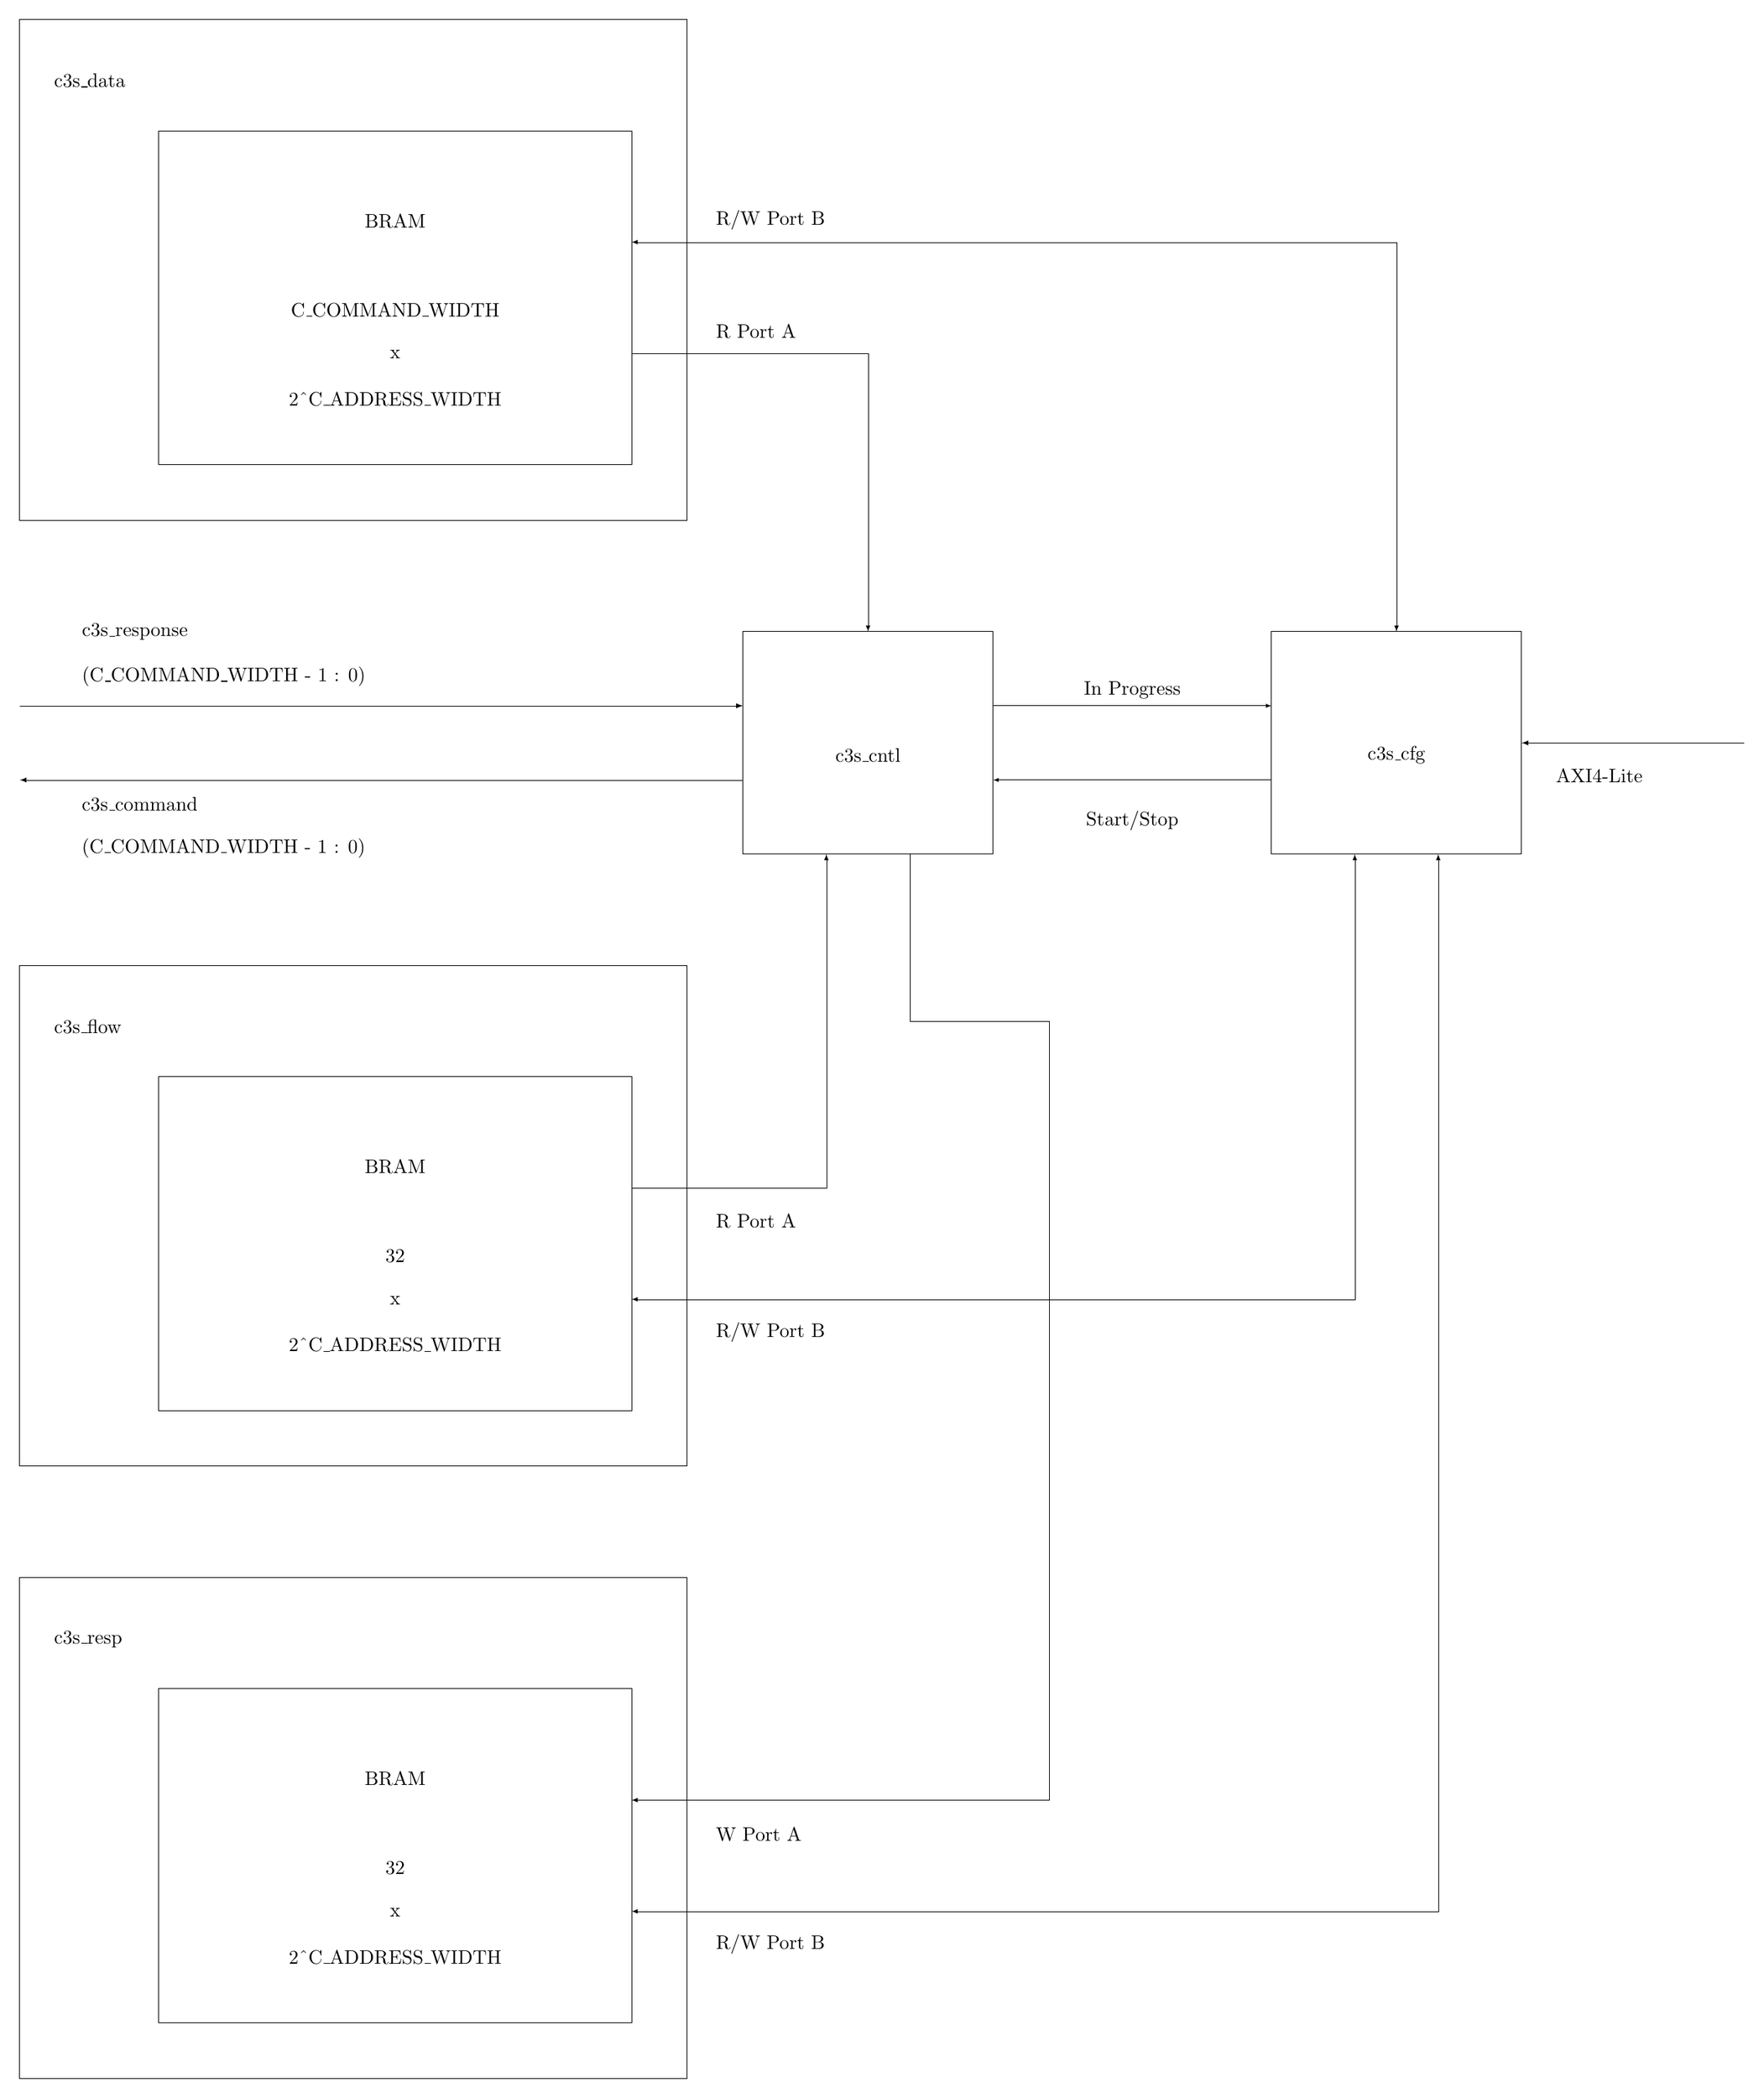
\begin{tikzpicture}
\pgftransformxscale{1.000000}
\pgftransformyscale{-1.000000}
\definecolor{dialinecolor}{rgb}{0.000000, 0.000000, 0.000000}
\pgfsetstrokecolor{dialinecolor}
\definecolor{dialinecolor}{rgb}{1.000000, 1.000000, 1.000000}
\pgfsetfillcolor{dialinecolor}
\pgfsetlinewidth{0.000000\du}
\pgfsetdash{}{0pt}
\pgfsetdash{}{0pt}
\pgfsetmiterjoin
\definecolor{dialinecolor}{rgb}{0.000000, 0.000000, 0.000000}
\pgfsetstrokecolor{dialinecolor}
\draw (21.000000\du,17.000000\du)--(21.000000\du,26.000000\du)--(33.000000\du,26.000000\du)--(33.000000\du,17.000000\du)--cycle;
% setfont left to latex
\definecolor{dialinecolor}{rgb}{0.000000, 0.000000, 0.000000}
\pgfsetstrokecolor{dialinecolor}
\node[anchor=west] at (21.500000\du,18.095000\du){c3s\_data};
\pgfsetlinewidth{0.000000\du}
\pgfsetdash{}{0pt}
\pgfsetdash{}{0pt}
\pgfsetmiterjoin
\definecolor{dialinecolor}{rgb}{0.000000, 0.000000, 0.000000}
\pgfsetstrokecolor{dialinecolor}
\draw (43.500000\du,28.000000\du)--(43.500000\du,32.000000\du)--(48.000000\du,32.000000\du)--(48.000000\du,28.000000\du)--cycle;
% setfont left to latex
\definecolor{dialinecolor}{rgb}{0.000000, 0.000000, 0.000000}
\pgfsetstrokecolor{dialinecolor}
\node at (45.750000\du,30.221250\du){c3s\_cfg};
\pgfsetlinewidth{0.000000\du}
\pgfsetdash{}{0pt}
\pgfsetdash{}{0pt}
\pgfsetmiterjoin
\definecolor{dialinecolor}{rgb}{0.000000, 0.000000, 0.000000}
\pgfsetstrokecolor{dialinecolor}
\draw (34.000000\du,28.000000\du)--(34.000000\du,32.000000\du)--(38.500000\du,32.000000\du)--(38.500000\du,28.000000\du)--cycle;
% setfont left to latex
\definecolor{dialinecolor}{rgb}{0.000000, 0.000000, 0.000000}
\pgfsetstrokecolor{dialinecolor}
\node at (36.250000\du,30.221250\du){c3s\_cntl};
\pgfsetlinewidth{0.000000\du}
\pgfsetdash{}{0pt}
\pgfsetdash{}{0pt}
\pgfsetmiterjoin
\definecolor{dialinecolor}{rgb}{0.000000, 0.000000, 0.000000}
\pgfsetstrokecolor{dialinecolor}
\draw (23.500000\du,19.000000\du)--(23.500000\du,25.000000\du)--(32.000000\du,25.000000\du)--(32.000000\du,19.000000\du)--cycle;
% setfont left to latex
\definecolor{dialinecolor}{rgb}{0.000000, 0.000000, 0.000000}
\pgfsetstrokecolor{dialinecolor}
\node at (27.750000\du,20.621050\du){BRAM};
% setfont left to latex
\definecolor{dialinecolor}{rgb}{0.000000, 0.000000, 0.000000}
\pgfsetstrokecolor{dialinecolor}
\node at (27.750000\du,21.421150\du){};
% setfont left to latex
\definecolor{dialinecolor}{rgb}{0.000000, 0.000000, 0.000000}
\pgfsetstrokecolor{dialinecolor}
\node at (27.750000\du,22.221250\du){C\_COMMAND\_WIDTH};
% setfont left to latex
\definecolor{dialinecolor}{rgb}{0.000000, 0.000000, 0.000000}
\pgfsetstrokecolor{dialinecolor}
\node at (27.750000\du,23.021350\du){x};
% setfont left to latex
\definecolor{dialinecolor}{rgb}{0.000000, 0.000000, 0.000000}
\pgfsetstrokecolor{dialinecolor}
\node at (27.750000\du,23.821450\du){2\^{}C\_ADDRESS\_WIDTH};
\pgfsetlinewidth{0.000000\du}
\pgfsetdash{}{0pt}
\pgfsetdash{}{0pt}
\pgfsetmiterjoin
\definecolor{dialinecolor}{rgb}{0.000000, 0.000000, 0.000000}
\pgfsetstrokecolor{dialinecolor}
\draw (21.000000\du,34.000000\du)--(21.000000\du,43.000000\du)--(33.000000\du,43.000000\du)--(33.000000\du,34.000000\du)--cycle;
% setfont left to latex
\definecolor{dialinecolor}{rgb}{0.000000, 0.000000, 0.000000}
\pgfsetstrokecolor{dialinecolor}
\node[anchor=west] at (21.500000\du,35.095000\du){c3s\_flow};
\pgfsetlinewidth{0.000000\du}
\pgfsetdash{}{0pt}
\pgfsetdash{}{0pt}
\pgfsetmiterjoin
\definecolor{dialinecolor}{rgb}{0.000000, 0.000000, 0.000000}
\pgfsetstrokecolor{dialinecolor}
\draw (23.500000\du,36.000000\du)--(23.500000\du,42.000000\du)--(32.000000\du,42.000000\du)--(32.000000\du,36.000000\du)--cycle;
% setfont left to latex
\definecolor{dialinecolor}{rgb}{0.000000, 0.000000, 0.000000}
\pgfsetstrokecolor{dialinecolor}
\node at (27.750000\du,37.621050\du){BRAM};
% setfont left to latex
\definecolor{dialinecolor}{rgb}{0.000000, 0.000000, 0.000000}
\pgfsetstrokecolor{dialinecolor}
\node at (27.750000\du,38.421150\du){};
% setfont left to latex
\definecolor{dialinecolor}{rgb}{0.000000, 0.000000, 0.000000}
\pgfsetstrokecolor{dialinecolor}
\node at (27.750000\du,39.221250\du){32};
% setfont left to latex
\definecolor{dialinecolor}{rgb}{0.000000, 0.000000, 0.000000}
\pgfsetstrokecolor{dialinecolor}
\node at (27.750000\du,40.021350\du){x};
% setfont left to latex
\definecolor{dialinecolor}{rgb}{0.000000, 0.000000, 0.000000}
\pgfsetstrokecolor{dialinecolor}
\node at (27.750000\du,40.821450\du){2\^{}C\_ADDRESS\_WIDTH};
\pgfsetlinewidth{0.100000\du}
\pgfsetdash{}{0pt}
\pgfsetdash{}{0pt}
\pgfsetmiterjoin
\pgfsetbuttcap
{
\definecolor{dialinecolor}{rgb}{0.000000, 0.000000, 0.000000}
\pgfsetfillcolor{dialinecolor}
% was here!!!
\pgfsetarrowsend{latex}
{\pgfsetcornersarced{\pgfpoint{0.000000\du}{0.000000\du}}\definecolor{dialinecolor}{rgb}{0.000000, 0.000000, 0.000000}
\pgfsetstrokecolor{dialinecolor}
\draw (32.000000\du,38.000000\du)--(35.500000\du,38.000000\du)--(35.500000\du,32.000000\du);
}}
\pgfsetlinewidth{0.100000\du}
\pgfsetdash{}{0pt}
\pgfsetdash{}{0pt}
\pgfsetmiterjoin
\pgfsetbuttcap
{
\definecolor{dialinecolor}{rgb}{0.000000, 0.000000, 0.000000}
\pgfsetfillcolor{dialinecolor}
% was here!!!
\pgfsetarrowsend{latex}
{\pgfsetcornersarced{\pgfpoint{0.000000\du}{0.000000\du}}\definecolor{dialinecolor}{rgb}{0.000000, 0.000000, 0.000000}
\pgfsetstrokecolor{dialinecolor}
\draw (32.000000\du,23.000000\du)--(36.250000\du,23.000000\du)--(36.250000\du,28.000000\du);
}}
\pgfsetlinewidth{0.000000\du}
\pgfsetdash{}{0pt}
\pgfsetdash{}{0pt}
\pgfsetbuttcap
{
\definecolor{dialinecolor}{rgb}{0.000000, 0.000000, 0.000000}
\pgfsetfillcolor{dialinecolor}
% was here!!!
\definecolor{dialinecolor}{rgb}{0.000000, 0.000000, 0.000000}
\pgfsetstrokecolor{dialinecolor}
\draw (32.000000\du,19.000000\du)--(32.000000\du,25.000000\du);
}
\pgfsetlinewidth{0.000000\du}
\pgfsetdash{}{0pt}
\pgfsetdash{}{0pt}
\pgfsetbuttcap
{
\definecolor{dialinecolor}{rgb}{0.000000, 0.000000, 0.000000}
\pgfsetfillcolor{dialinecolor}
% was here!!!
\definecolor{dialinecolor}{rgb}{0.000000, 0.000000, 0.000000}
\pgfsetstrokecolor{dialinecolor}
\draw (32.000000\du,36.000000\du)--(32.000000\du,42.000000\du);
}
\pgfsetlinewidth{0.100000\du}
\pgfsetdash{}{0pt}
\pgfsetdash{}{0pt}
\pgfsetmiterjoin
\pgfsetbuttcap
{
\definecolor{dialinecolor}{rgb}{0.000000, 0.000000, 0.000000}
\pgfsetfillcolor{dialinecolor}
% was here!!!
\pgfsetarrowsstart{latex}
\pgfsetarrowsend{latex}
{\pgfsetcornersarced{\pgfpoint{0.000000\du}{0.000000\du}}\definecolor{dialinecolor}{rgb}{0.000000, 0.000000, 0.000000}
\pgfsetstrokecolor{dialinecolor}
\draw (32.000000\du,21.000000\du)--(45.750000\du,21.000000\du)--(45.750000\du,28.000000\du);
}}
% setfont left to latex
\definecolor{dialinecolor}{rgb}{0.000000, 0.000000, 0.000000}
\pgfsetstrokecolor{dialinecolor}
\node[anchor=west] at (33.400000\du,20.600000\du){R/W Port B};
% setfont left to latex
\definecolor{dialinecolor}{rgb}{0.000000, 0.000000, 0.000000}
\pgfsetstrokecolor{dialinecolor}
\node[anchor=west] at (33.400000\du,22.600000\du){R Port A};
% setfont left to latex
\definecolor{dialinecolor}{rgb}{0.000000, 0.000000, 0.000000}
\pgfsetstrokecolor{dialinecolor}
\node[anchor=west] at (33.400000\du,40.595000\du){R/W Port B};
% setfont left to latex
\definecolor{dialinecolor}{rgb}{0.000000, 0.000000, 0.000000}
\pgfsetstrokecolor{dialinecolor}
\node[anchor=west] at (33.400000\du,38.595000\du){R Port A};
\pgfsetlinewidth{0.100000\du}
\pgfsetdash{}{0pt}
\pgfsetdash{}{0pt}
\pgfsetmiterjoin
\pgfsetbuttcap
{
\definecolor{dialinecolor}{rgb}{0.000000, 0.000000, 0.000000}
\pgfsetfillcolor{dialinecolor}
% was here!!!
\pgfsetarrowsstart{latex}
\pgfsetarrowsend{latex}
{\pgfsetcornersarced{\pgfpoint{0.000000\du}{0.000000\du}}\definecolor{dialinecolor}{rgb}{0.000000, 0.000000, 0.000000}
\pgfsetstrokecolor{dialinecolor}
\draw (32.000000\du,40.000000\du)--(45.000000\du,40.000000\du)--(45.000000\du,32.000000\du);
}}
% setfont left to latex
\definecolor{dialinecolor}{rgb}{0.000000, 0.000000, 0.000000}
\pgfsetstrokecolor{dialinecolor}
\node at (41.000000\du,31.395000\du){Start/Stop};
\pgfsetlinewidth{0.000000\du}
\pgfsetdash{}{0pt}
\pgfsetdash{}{0pt}
\pgfsetbuttcap
{
\definecolor{dialinecolor}{rgb}{0.000000, 0.000000, 0.000000}
\pgfsetfillcolor{dialinecolor}
% was here!!!
\definecolor{dialinecolor}{rgb}{0.000000, 0.000000, 0.000000}
\pgfsetstrokecolor{dialinecolor}
\draw (38.500000\du,28.000000\du)--(38.500000\du,32.000000\du);
}
\pgfsetlinewidth{0.000000\du}
\pgfsetdash{}{0pt}
\pgfsetdash{}{0pt}
\pgfsetbuttcap
{
\definecolor{dialinecolor}{rgb}{0.000000, 0.000000, 0.000000}
\pgfsetfillcolor{dialinecolor}
% was here!!!
\definecolor{dialinecolor}{rgb}{0.000000, 0.000000, 0.000000}
\pgfsetstrokecolor{dialinecolor}
\draw (43.500000\du,28.000000\du)--(43.500000\du,32.000000\du);
}
% setfont left to latex
\definecolor{dialinecolor}{rgb}{0.000000, 0.000000, 0.000000}
\pgfsetstrokecolor{dialinecolor}
\node at (41.000000\du,29.047500\du){In Progress};
% setfont left to latex
\definecolor{dialinecolor}{rgb}{0.000000, 0.000000, 0.000000}
\pgfsetstrokecolor{dialinecolor}
\node[anchor=west] at (22.000000\du,31.095000\du){c3s\_command};
% setfont left to latex
\definecolor{dialinecolor}{rgb}{0.000000, 0.000000, 0.000000}
\pgfsetstrokecolor{dialinecolor}
\node[anchor=west] at (22.000000\du,31.895000\du){      (C\_COMMAND\_WIDTH - 1 : 0)};
% setfont left to latex
\definecolor{dialinecolor}{rgb}{0.000000, 0.000000, 0.000000}
\pgfsetstrokecolor{dialinecolor}
\node[anchor=west] at (48.500000\du,30.595000\du){AXI4-Lite};
\pgfsetlinewidth{0.000000\du}
\pgfsetdash{}{0pt}
\pgfsetdash{}{0pt}
\pgfsetbuttcap
{
\definecolor{dialinecolor}{rgb}{0.000000, 0.000000, 0.000000}
\pgfsetfillcolor{dialinecolor}
% was here!!!
\pgfsetarrowsend{latex}
\definecolor{dialinecolor}{rgb}{0.000000, 0.000000, 0.000000}
\pgfsetstrokecolor{dialinecolor}
\draw (38.500000\du,29.333300\du)--(43.500000\du,29.333300\du);
}
\pgfsetlinewidth{0.000000\du}
\pgfsetdash{}{0pt}
\pgfsetdash{}{0pt}
\pgfsetbuttcap
{
\definecolor{dialinecolor}{rgb}{0.000000, 0.000000, 0.000000}
\pgfsetfillcolor{dialinecolor}
% was here!!!
\pgfsetarrowsend{latex}
\definecolor{dialinecolor}{rgb}{0.000000, 0.000000, 0.000000}
\pgfsetstrokecolor{dialinecolor}
\draw (43.500000\du,30.666700\du)--(38.500000\du,30.666700\du);
}
\pgfsetlinewidth{0.200000\du}
\pgfsetdash{}{0pt}
\pgfsetdash{}{0pt}
\pgfsetbuttcap
{
\definecolor{dialinecolor}{rgb}{0.000000, 0.000000, 0.000000}
\pgfsetfillcolor{dialinecolor}
% was here!!!
\pgfsetarrowsend{latex}
\definecolor{dialinecolor}{rgb}{0.000000, 0.000000, 0.000000}
\pgfsetstrokecolor{dialinecolor}
\draw (52.000000\du,30.000000\du)--(48.000000\du,30.000000\du);
}
\pgfsetlinewidth{0.200000\du}
\pgfsetdash{}{0pt}
\pgfsetdash{}{0pt}
\pgfsetbuttcap
{
\definecolor{dialinecolor}{rgb}{0.000000, 0.000000, 0.000000}
\pgfsetfillcolor{dialinecolor}
% was here!!!
\pgfsetarrowsend{latex}
\definecolor{dialinecolor}{rgb}{0.000000, 0.000000, 0.000000}
\pgfsetstrokecolor{dialinecolor}
\draw (34.000000\du,30.666667\du)--(21.000000\du,30.666667\du);
}
\pgfsetlinewidth{0.000000\du}
\pgfsetdash{}{0pt}
\pgfsetdash{}{0pt}
\pgfsetbuttcap
{
\definecolor{dialinecolor}{rgb}{0.000000, 0.000000, 0.000000}
\pgfsetfillcolor{dialinecolor}
% was here!!!
\definecolor{dialinecolor}{rgb}{0.000000, 0.000000, 0.000000}
\pgfsetstrokecolor{dialinecolor}
\draw (34.000000\du,32.000000\du)--(38.500000\du,32.000000\du);
}
\pgfsetlinewidth{0.000000\du}
\pgfsetdash{}{0pt}
\pgfsetdash{}{0pt}
\pgfsetbuttcap
{
\definecolor{dialinecolor}{rgb}{0.000000, 0.000000, 0.000000}
\pgfsetfillcolor{dialinecolor}
% was here!!!
\definecolor{dialinecolor}{rgb}{0.000000, 0.000000, 0.000000}
\pgfsetstrokecolor{dialinecolor}
\draw (34.000000\du,28.000000\du)--(34.000000\du,32.000000\du);
}
\pgfsetlinewidth{0.200000\du}
\pgfsetdash{}{0pt}
\pgfsetdash{}{0pt}
\pgfsetbuttcap
{
\definecolor{dialinecolor}{rgb}{0.000000, 0.000000, 0.000000}
\pgfsetfillcolor{dialinecolor}
% was here!!!
\pgfsetarrowsend{latex}
\definecolor{dialinecolor}{rgb}{0.000000, 0.000000, 0.000000}
\pgfsetstrokecolor{dialinecolor}
\draw (21.000000\du,29.333333\du)--(34.000000\du,29.333333\du);
}
% setfont left to latex
\definecolor{dialinecolor}{rgb}{0.000000, 0.000000, 0.000000}
\pgfsetstrokecolor{dialinecolor}
\node[anchor=west] at (22.000000\du,28.010125\du){c3s\_response};
% setfont left to latex
\definecolor{dialinecolor}{rgb}{0.000000, 0.000000, 0.000000}
\pgfsetstrokecolor{dialinecolor}
\node[anchor=west] at (22.000000\du,28.810125\du){      (C\_COMMAND\_WIDTH - 1 : 0)};
\pgfsetlinewidth{0.000000\du}
\pgfsetdash{}{0pt}
\pgfsetdash{}{0pt}
\pgfsetmiterjoin
\definecolor{dialinecolor}{rgb}{0.000000, 0.000000, 0.000000}
\pgfsetstrokecolor{dialinecolor}
\draw (21.000000\du,45.000000\du)--(21.000000\du,54.000000\du)--(33.000000\du,54.000000\du)--(33.000000\du,45.000000\du)--cycle;
% setfont left to latex
\definecolor{dialinecolor}{rgb}{0.000000, 0.000000, 0.000000}
\pgfsetstrokecolor{dialinecolor}
\node[anchor=west] at (21.500000\du,46.113687\du){c3s\_resp};
\pgfsetlinewidth{0.000000\du}
\pgfsetdash{}{0pt}
\pgfsetdash{}{0pt}
\pgfsetmiterjoin
\definecolor{dialinecolor}{rgb}{0.000000, 0.000000, 0.000000}
\pgfsetstrokecolor{dialinecolor}
\draw (23.500000\du,47.000000\du)--(23.500000\du,53.000000\du)--(32.000000\du,53.000000\du)--(32.000000\du,47.000000\du)--cycle;
% setfont left to latex
\definecolor{dialinecolor}{rgb}{0.000000, 0.000000, 0.000000}
\pgfsetstrokecolor{dialinecolor}
\node at (27.750000\du,48.621050\du){BRAM};
% setfont left to latex
\definecolor{dialinecolor}{rgb}{0.000000, 0.000000, 0.000000}
\pgfsetstrokecolor{dialinecolor}
\node at (27.750000\du,49.421150\du){};
% setfont left to latex
\definecolor{dialinecolor}{rgb}{0.000000, 0.000000, 0.000000}
\pgfsetstrokecolor{dialinecolor}
\node at (27.750000\du,50.221250\du){32};
% setfont left to latex
\definecolor{dialinecolor}{rgb}{0.000000, 0.000000, 0.000000}
\pgfsetstrokecolor{dialinecolor}
\node at (27.750000\du,51.021350\du){x};
% setfont left to latex
\definecolor{dialinecolor}{rgb}{0.000000, 0.000000, 0.000000}
\pgfsetstrokecolor{dialinecolor}
\node at (27.750000\du,51.821450\du){2\^{}C\_ADDRESS\_WIDTH};
\pgfsetlinewidth{0.100000\du}
\pgfsetdash{}{0pt}
\pgfsetdash{}{0pt}
\pgfsetmiterjoin
\pgfsetbuttcap
{
\definecolor{dialinecolor}{rgb}{0.000000, 0.000000, 0.000000}
\pgfsetfillcolor{dialinecolor}
% was here!!!
\pgfsetarrowsend{latex}
{\pgfsetcornersarced{\pgfpoint{0.000000\du}{0.000000\du}}\definecolor{dialinecolor}{rgb}{0.000000, 0.000000, 0.000000}
\pgfsetstrokecolor{dialinecolor}
\draw (37.000000\du,32.000000\du)--(37.000000\du,35.000000\du)--(39.500000\du,35.000000\du)--(39.500000\du,49.000000\du)--(32.000000\du,49.000000\du);
}}
\pgfsetlinewidth{0.000000\du}
\pgfsetdash{}{0pt}
\pgfsetdash{}{0pt}
\pgfsetbuttcap
{
\definecolor{dialinecolor}{rgb}{0.000000, 0.000000, 0.000000}
\pgfsetfillcolor{dialinecolor}
% was here!!!
\definecolor{dialinecolor}{rgb}{0.000000, 0.000000, 0.000000}
\pgfsetstrokecolor{dialinecolor}
\draw (32.000000\du,47.000000\du)--(32.000000\du,53.000000\du);
}
% setfont left to latex
\definecolor{dialinecolor}{rgb}{0.000000, 0.000000, 0.000000}
\pgfsetstrokecolor{dialinecolor}
\node[anchor=west] at (33.400000\du,51.595000\du){R/W Port B};
% setfont left to latex
\definecolor{dialinecolor}{rgb}{0.000000, 0.000000, 0.000000}
\pgfsetstrokecolor{dialinecolor}
\node[anchor=west] at (33.400000\du,49.613687\du){W Port A};
\pgfsetlinewidth{0.100000\du}
\pgfsetdash{}{0pt}
\pgfsetdash{}{0pt}
\pgfsetmiterjoin
\pgfsetbuttcap
{
\definecolor{dialinecolor}{rgb}{0.000000, 0.000000, 0.000000}
\pgfsetfillcolor{dialinecolor}
% was here!!!
\pgfsetarrowsstart{latex}
\pgfsetarrowsend{latex}
{\pgfsetcornersarced{\pgfpoint{0.000000\du}{0.000000\du}}\definecolor{dialinecolor}{rgb}{0.000000, 0.000000, 0.000000}
\pgfsetstrokecolor{dialinecolor}
\draw (32.000000\du,51.000000\du)--(46.500000\du,51.000000\du)--(46.500000\du,32.000000\du);
}}
\pgfsetlinewidth{0.000000\du}
\pgfsetdash{}{0pt}
\pgfsetdash{}{0pt}
\pgfsetbuttcap
{
\definecolor{dialinecolor}{rgb}{0.000000, 0.000000, 0.000000}
\pgfsetfillcolor{dialinecolor}
% was here!!!
\definecolor{dialinecolor}{rgb}{0.000000, 0.000000, 0.000000}
\pgfsetstrokecolor{dialinecolor}
\draw (43.500000\du,32.000000\du)--(48.000000\du,32.000000\du);
}
\end{tikzpicture}

  \end{center}
  \caption[Overview of c3s\_rlm.vhdl]{\label{fig:c3s_overview}Overview of c3s\_rlm.vhdl
  }
\end{figure}

\subsection{Interfaces}
VHDL Name: c3s\_rlm (c3s\_rlm.vhdl)

\subsubsection{Generics}
\begin{center}
  \begin{tabular}{ l | c | c | c | c | p{.3\linewidth} }
    Generic Name      & Type     & Min & Max  & Default & Description \\
    \hline
    C\_COMMAND\_WIDTH & Positive & 1   & 8192 & 512     & Number of bits in command driven by C3S. A multiple of 32 is required for efficient implementation. \\
    \hline
    C\_ADDRESS\_WIDTH & Positive & 1   & 8    & 5       & Command array will contain 2\textsuperscript{C\_ADDRESS\_WIDTH} commands. \\
  \end{tabular}
\end{center}

\subsubsection{Ports}
\begin{center}
  \begin{tabular}{ l | c | c | p{.3\linewidth} }
    Signal Name          & I/O & Size              & Description \\
    \hline
    \multicolumn{4}{c}{Clocking} \\
    \hline
    clock                & I   & 1                 & Positive clock \\
    \hline
    reset                & I   & 1                 & Active-high reset \\
    \hline
    \multicolumn{4}{c}{Command} \\
    \hline
    c3s\_command         & O   & C\_COMMAND\_WIDTH & C3S command vector \\
    \hline
    c3s\_command\_valid  & O   & 1                 & C3S command is valid, optional and custom use \\
    \hline
    c3s\_command\_sel    & O   & 1                 & Asserted high when C3S is running and commands are valid \\
    \hline
    \multicolumn{4}{c}{Response} \\
    \hline
    c3s\_response        & I   & C\_COMMAND\_WIDTH & C3S response vector \\
    \hline
    c3s\_response\_valid & I   & 1                 & Response is valid and should be stored in response array \\
  \end{tabular}
\end{center}

\textbf{Note}: Signals are little-endian ($N$ \textbf{downto} 0)

\subsection{Data Array}
VHDL Name: c3s\_data(bram\_wrap.vhdl)

The data array is simply a C\_COMMAND\_WIDTH wide by
2\textsuperscript{C\_ADDRESS\_WIDTH} deep array that contains the
instructions. Each bit of a row corresponds one-to-one with each bit
of c3s\_command, and each row is a discrete command. The Instruction
Flow Array controls exactly how these commands are sent.

The array is implemented as a BRAM (Block RAM) primitive with 2 R/W
ports. Port A is connected to the control block which does reads
during C3S execution. The control block does not do writes. Port B is
connected to the configuration block for read and write configurations
over AXI4-Lite, where each row of the data array is one or more unique
register(s).

\begin{emulation}
In an emulation environment, BRAM primitives are not available in the
hardware, as they are specific for Xilinx FPGAs like that used on
Apollo. The BRAM wrapper, bram\_wrap.vhdl, is designed to infer
latches if it's in an environment without BRAM devices.
\end{emulation}

\subsection{Response Capture Array}
VHDL Name: c3s\_resp(bram\_wrap.vhdl)

The response capture array provides a method to see the responses
coming across an interface. No checking is done; rather the responses
are inserted into the array for manual analysis. The array is written
to by an incrementing write pointer. When the maximum value of the
write pointer is reached, it resets to 0 and starts overwriting
previous entries. This ensures that the most recent responses received
are found in the array. When a response is stored in the array, there
is also a timestamp stored. This measures the time from the start of
C3S execution to when the response was received by the Response
Capture Array.

The C3S\_RESP\_CNTL provides a method to see where in the array we are
writing, if we have wrapper around. There is also a way to reset the
write address to start counting from 0 in order to provide a higher
chance of a repeatable test.

This array is the same size as the data array: C\_COMMAND\_WIDTH wide
by 2\textsuperscript{C\_ADDRESS\_WIDTH} deep.

There is a wrap path inside the control block that allows c3s\_command
to be written into the response array rather than c3s\_response. This
allows debug of a C3S sequence to verify the commands being sent
without relying on the interface. Additionally, it is possible to
disable c3s\_command\_sel in order to capture the command without
actually sending anything across the interface, in order to not
interfere with real traffic. Both of these settings are configurable
in C3S\_CNTL.

\subsection{Instruction Flow Array}
VHDL Name: c3s\_flow(bram\_wrap.vhdl)

The instruction flow array is the meta information associated with
each data entry. The array is a constant 32 bits wide by
2\textsuperscript{C\_ADDRESS\_WIDTH} deep. This flow entry contains a
repeat flag, a next instruction pointer, and a last entry flag. The
repeat flag indicates that a command repeats a number of times. Each
command is run one more than than the number gives, e.g. 0 means the
command will run only once, 1 means the command is repeated twice. The
next instruction pointer points to the command that will run next. If
set to the next address, execution will serially go through the
array. This also allows infinite loops. Finally, if execution sees a
command with the last entry flag, then C3S execution will
stop. Currently, the command containing the last entry flag is not
executed, so the final command executed is the command before the one
with the last entry flag set.

\subsection{Control Block}
VHDL Name: c3s\_cntl(c3s\_cntl.vhdl)

The control block is the core of C3S that performs a few functions. It
contains the central state machine, the read controls for port A of
the flow and data, and write controls for port A of the response. The
state machine, outlined in Figure~\ref{fig:c3s_fsm}, steps through the
C3S array as programmed by the Instruction Flow Array and forwards the
command in the Data Array to the command bus. States are encode in a
one-hot signal, with c3s\_fsm\_q(0) being set for state 0, and so
on. Additionally, the control block contains the write logic for the
response array, writing to the response array only when the response
is valid.

\begin{figure}[h]
  \begin{center}
    % Graphic for TeX using PGF
% Title: /afs/apd/func/vlsi/eclipz/c14/usr/rpking42/cbdd1/astra-sim/doc/images/c3s_fsm.dia
% Creator: Dia v0.97.3
% CreationDate: Tue Jun 12 17:56:29 2018
% For: rpking42
% \usepackage{tikz}
% The following commands are not supported in PSTricks at present
% We define them conditionally, so when they are implemented,
% this pgf file will use them.
\ifx\du\undefined
  \newlength{\du}
\fi
\setlength{\du}{15\unitlength}
\begin{tikzpicture}
\pgftransformxscale{1.000000}
\pgftransformyscale{-1.000000}
\definecolor{dialinecolor}{rgb}{0.000000, 0.000000, 0.000000}
\pgfsetstrokecolor{dialinecolor}
\definecolor{dialinecolor}{rgb}{1.000000, 1.000000, 1.000000}
\pgfsetfillcolor{dialinecolor}
\definecolor{dialinecolor}{rgb}{1.000000, 1.000000, 1.000000}
\pgfsetfillcolor{dialinecolor}
\pgfpathellipse{\pgfpoint{14.500000\du}{11.500000\du}}{\pgfpoint{2.500000\du}{0\du}}{\pgfpoint{0\du}{2.500000\du}}
\pgfusepath{fill}
\pgfsetlinewidth{0.000000\du}
\pgfsetdash{}{0pt}
\pgfsetdash{}{0pt}
\definecolor{dialinecolor}{rgb}{0.000000, 0.000000, 0.000000}
\pgfsetstrokecolor{dialinecolor}
\pgfpathellipse{\pgfpoint{14.500000\du}{11.500000\du}}{\pgfpoint{2.500000\du}{0\du}}{\pgfpoint{0\du}{2.500000\du}}
\pgfusepath{stroke}
\definecolor{dialinecolor}{rgb}{1.000000, 1.000000, 1.000000}
\pgfsetfillcolor{dialinecolor}
\pgfpathellipse{\pgfpoint{24.500000\du}{11.500000\du}}{\pgfpoint{2.500000\du}{0\du}}{\pgfpoint{0\du}{2.500000\du}}
\pgfusepath{fill}
\pgfsetlinewidth{0.000000\du}
\pgfsetdash{}{0pt}
\pgfsetdash{}{0pt}
\definecolor{dialinecolor}{rgb}{0.000000, 0.000000, 0.000000}
\pgfsetstrokecolor{dialinecolor}
\pgfpathellipse{\pgfpoint{24.500000\du}{11.500000\du}}{\pgfpoint{2.500000\du}{0\du}}{\pgfpoint{0\du}{2.500000\du}}
\pgfusepath{stroke}
\definecolor{dialinecolor}{rgb}{1.000000, 1.000000, 1.000000}
\pgfsetfillcolor{dialinecolor}
\pgfpathellipse{\pgfpoint{14.500000\du}{21.500000\du}}{\pgfpoint{2.500000\du}{0\du}}{\pgfpoint{0\du}{2.500000\du}}
\pgfusepath{fill}
\pgfsetlinewidth{0.000000\du}
\pgfsetdash{}{0pt}
\pgfsetdash{}{0pt}
\definecolor{dialinecolor}{rgb}{0.000000, 0.000000, 0.000000}
\pgfsetstrokecolor{dialinecolor}
\pgfpathellipse{\pgfpoint{14.500000\du}{21.500000\du}}{\pgfpoint{2.500000\du}{0\du}}{\pgfpoint{0\du}{2.500000\du}}
\pgfusepath{stroke}
\definecolor{dialinecolor}{rgb}{1.000000, 1.000000, 1.000000}
\pgfsetfillcolor{dialinecolor}
\pgfpathellipse{\pgfpoint{24.500000\du}{21.500000\du}}{\pgfpoint{2.500000\du}{0\du}}{\pgfpoint{0\du}{2.500000\du}}
\pgfusepath{fill}
\pgfsetlinewidth{0.000000\du}
\pgfsetdash{}{0pt}
\pgfsetdash{}{0pt}
\definecolor{dialinecolor}{rgb}{0.000000, 0.000000, 0.000000}
\pgfsetstrokecolor{dialinecolor}
\pgfpathellipse{\pgfpoint{24.500000\du}{21.500000\du}}{\pgfpoint{2.500000\du}{0\du}}{\pgfpoint{0\du}{2.500000\du}}
\pgfusepath{stroke}
% setfont left to latex
\definecolor{dialinecolor}{rgb}{0.000000, 0.000000, 0.000000}
\pgfsetstrokecolor{dialinecolor}
\node at (14.500000\du,10.921250\du){State 0};
% setfont left to latex
\definecolor{dialinecolor}{rgb}{0.000000, 0.000000, 0.000000}
\pgfsetstrokecolor{dialinecolor}
\node at (14.500000\du,11.721250\du){};
% setfont left to latex
\definecolor{dialinecolor}{rgb}{0.000000, 0.000000, 0.000000}
\pgfsetstrokecolor{dialinecolor}
\node at (14.500000\du,12.521250\du){Idle};
% setfont left to latex
\definecolor{dialinecolor}{rgb}{0.000000, 0.000000, 0.000000}
\pgfsetstrokecolor{dialinecolor}
\node at (24.500000\du,10.521250\du){State 1};
% setfont left to latex
\definecolor{dialinecolor}{rgb}{0.000000, 0.000000, 0.000000}
\pgfsetstrokecolor{dialinecolor}
\node at (24.500000\du,11.321250\du){};
% setfont left to latex
\definecolor{dialinecolor}{rgb}{0.000000, 0.000000, 0.000000}
\pgfsetstrokecolor{dialinecolor}
\node at (24.500000\du,12.121250\du){Send};
% setfont left to latex
\definecolor{dialinecolor}{rgb}{0.000000, 0.000000, 0.000000}
\pgfsetstrokecolor{dialinecolor}
\node at (24.500000\du,12.921250\du){Instruction};
% setfont left to latex
\definecolor{dialinecolor}{rgb}{0.000000, 0.000000, 0.000000}
\pgfsetstrokecolor{dialinecolor}
\node at (14.500000\du,20.921250\du){State 2};
% setfont left to latex
\definecolor{dialinecolor}{rgb}{0.000000, 0.000000, 0.000000}
\pgfsetstrokecolor{dialinecolor}
\node at (14.500000\du,21.721250\du){};
% setfont left to latex
\definecolor{dialinecolor}{rgb}{0.000000, 0.000000, 0.000000}
\pgfsetstrokecolor{dialinecolor}
\node at (14.500000\du,22.521250\du){Done};
% setfont left to latex
\definecolor{dialinecolor}{rgb}{0.000000, 0.000000, 0.000000}
\pgfsetstrokecolor{dialinecolor}
\node at (24.500000\du,20.921250\du){State 3};
% setfont left to latex
\definecolor{dialinecolor}{rgb}{0.000000, 0.000000, 0.000000}
\pgfsetstrokecolor{dialinecolor}
\node at (24.500000\du,21.721250\du){};
% setfont left to latex
\definecolor{dialinecolor}{rgb}{0.000000, 0.000000, 0.000000}
\pgfsetstrokecolor{dialinecolor}
\node at (24.500000\du,22.521250\du){Repeat};
\pgfsetlinewidth{0.000000\du}
\pgfsetdash{}{0pt}
\pgfsetdash{}{0pt}
\pgfsetbuttcap
{
\definecolor{dialinecolor}{rgb}{0.000000, 0.000000, 0.000000}
\pgfsetfillcolor{dialinecolor}
% was here!!!
\pgfsetarrowsend{latex}
\definecolor{dialinecolor}{rgb}{0.000000, 0.000000, 0.000000}
\pgfsetstrokecolor{dialinecolor}
\draw (9.000000\du,11.500000\du)--(12.000000\du,11.500000\du);
}
\pgfsetlinewidth{0.000000\du}
\pgfsetdash{}{0pt}
\pgfsetdash{}{0pt}
\pgfsetbuttcap
{
\definecolor{dialinecolor}{rgb}{0.000000, 0.000000, 0.000000}
\pgfsetfillcolor{dialinecolor}
% was here!!!
\pgfsetarrowsend{latex}
\definecolor{dialinecolor}{rgb}{0.000000, 0.000000, 0.000000}
\pgfsetstrokecolor{dialinecolor}
\draw (17.000000\du,11.500000\du)--(22.000000\du,11.500000\du);
}
\pgfsetlinewidth{0.000000\du}
\pgfsetdash{}{0pt}
\pgfsetdash{}{0pt}
\pgfsetbuttcap
{
\definecolor{dialinecolor}{rgb}{0.000000, 0.000000, 0.000000}
\pgfsetfillcolor{dialinecolor}
% was here!!!
\pgfsetarrowsend{latex}
\definecolor{dialinecolor}{rgb}{0.000000, 0.000000, 0.000000}
\pgfsetstrokecolor{dialinecolor}
\pgfpathmoveto{\pgfpoint{14.499995\du}{9.000110\du}}
\pgfpatharc{3}{-227}{1.054486\du and 1.054486\du}
\pgfusepath{stroke}
}
% setfont left to latex
\definecolor{dialinecolor}{rgb}{0.000000, 0.000000, 0.000000}
\pgfsetstrokecolor{dialinecolor}
\node[anchor=west] at (9.000000\du,11.000000\du){reset};
% setfont left to latex
\definecolor{dialinecolor}{rgb}{0.000000, 0.000000, 0.000000}
\pgfsetstrokecolor{dialinecolor}
\node[anchor=west] at (17.500000\du,11.000000\du){c3s\_start};
% setfont left to latex
\definecolor{dialinecolor}{rgb}{0.000000, 0.000000, 0.000000}
\pgfsetstrokecolor{dialinecolor}
\node[anchor=west] at (11.000000\du,7.500000\du){! c3s\_start};
\pgfsetlinewidth{0.000000\du}
\pgfsetdash{}{0pt}
\pgfsetdash{}{0pt}
\pgfsetbuttcap
{
\definecolor{dialinecolor}{rgb}{0.000000, 0.000000, 0.000000}
\pgfsetfillcolor{dialinecolor}
% was here!!!
\pgfsetarrowsend{latex}
\definecolor{dialinecolor}{rgb}{0.000000, 0.000000, 0.000000}
\pgfsetstrokecolor{dialinecolor}
\draw (24.500000\du,14.000000\du)--(24.500000\du,19.000000\du);
}
\pgfsetlinewidth{0.000000\du}
\pgfsetdash{}{0pt}
\pgfsetdash{}{0pt}
\pgfsetbuttcap
{
\definecolor{dialinecolor}{rgb}{0.000000, 0.000000, 0.000000}
\pgfsetfillcolor{dialinecolor}
% was here!!!
\pgfsetarrowsend{latex}
\definecolor{dialinecolor}{rgb}{0.000000, 0.000000, 0.000000}
\pgfsetstrokecolor{dialinecolor}
\draw (22.732200\du,13.267800\du)--(16.267800\du,19.732200\du);
}
\pgfsetlinewidth{0.000000\du}
\pgfsetdash{}{0pt}
\pgfsetdash{}{0pt}
\pgfsetbuttcap
{
\definecolor{dialinecolor}{rgb}{0.000000, 0.000000, 0.000000}
\pgfsetfillcolor{dialinecolor}
% was here!!!
\pgfsetarrowsend{latex}
\definecolor{dialinecolor}{rgb}{0.000000, 0.000000, 0.000000}
\pgfsetstrokecolor{dialinecolor}
\pgfpathmoveto{\pgfpoint{26.267722\du}{9.732404\du}}
\pgfpatharc{25}{-204}{1.938014\du and 1.938014\du}
\pgfusepath{stroke}
}
% setfont left to latex
\definecolor{dialinecolor}{rgb}{0.000000, 0.000000, 0.000000}
\pgfsetstrokecolor{dialinecolor}
\node[anchor=west] at (19.000000\du,5.500000\du){! last instruction AND};
% setfont left to latex
\definecolor{dialinecolor}{rgb}{0.000000, 0.000000, 0.000000}
\pgfsetstrokecolor{dialinecolor}
\node[anchor=west] at (19.000000\du,6.300000\du){repeat\_count == 0};
% setfont left to latex
\definecolor{dialinecolor}{rgb}{0.000000, 0.000000, 0.000000}
\pgfsetstrokecolor{dialinecolor}
\node[anchor=west] at (16.500000\du,17.500000\du){last instruction};
\pgfsetlinewidth{0.000000\du}
\pgfsetdash{}{0pt}
\pgfsetdash{}{0pt}
\pgfsetbuttcap
{
\definecolor{dialinecolor}{rgb}{0.000000, 0.000000, 0.000000}
\pgfsetfillcolor{dialinecolor}
% was here!!!
\pgfsetarrowsend{latex}
\definecolor{dialinecolor}{rgb}{0.000000, 0.000000, 0.000000}
\pgfsetstrokecolor{dialinecolor}
\draw (14.500000\du,19.000000\du)--(14.500000\du,14.000000\du);
}
\pgfsetlinewidth{0.000000\du}
\pgfsetdash{}{0pt}
\pgfsetdash{}{0pt}
\pgfsetbuttcap
{
\definecolor{dialinecolor}{rgb}{0.000000, 0.000000, 0.000000}
\pgfsetfillcolor{dialinecolor}
% was here!!!
\pgfsetarrowsend{latex}
\definecolor{dialinecolor}{rgb}{0.000000, 0.000000, 0.000000}
\pgfsetstrokecolor{dialinecolor}
\pgfpathmoveto{\pgfpoint{26.267492\du}{19.732650\du}}
\pgfpatharc{35}{-34}{5.723558\du and 5.723558\du}
\pgfusepath{stroke}
}
\pgfsetlinewidth{0.000000\du}
\pgfsetdash{}{0pt}
\pgfsetdash{}{0pt}
\pgfsetbuttcap
{
\definecolor{dialinecolor}{rgb}{0.000000, 0.000000, 0.000000}
\pgfsetfillcolor{dialinecolor}
% was here!!!
\pgfsetarrowsend{latex}
\definecolor{dialinecolor}{rgb}{0.000000, 0.000000, 0.000000}
\pgfsetstrokecolor{dialinecolor}
\pgfpathmoveto{\pgfpoint{24.500002\du}{23.999945\du}}
\pgfpatharc{183}{-47}{1.054482\du and 1.054482\du}
\pgfusepath{stroke}
}
% setfont left to latex
\definecolor{dialinecolor}{rgb}{0.000000, 0.000000, 0.000000}
\pgfsetstrokecolor{dialinecolor}
\node[anchor=west] at (27.000000\du,19.000000\du){repeat\_count\_int == 0};
% setfont left to latex
\definecolor{dialinecolor}{rgb}{0.000000, 0.000000, 0.000000}
\pgfsetstrokecolor{dialinecolor}
\node[anchor=west] at (22.000000\du,26.000000\du){repeat\_count\_int != 0};
% setfont left to latex
\definecolor{dialinecolor}{rgb}{0.000000, 0.000000, 0.000000}
\pgfsetstrokecolor{dialinecolor}
\node[anchor=west] at (21.000000\du,15.500000\du){! last instruction AND};
% setfont left to latex
\definecolor{dialinecolor}{rgb}{0.000000, 0.000000, 0.000000}
\pgfsetstrokecolor{dialinecolor}
\node[anchor=west] at (21.000000\du,16.300000\du){repeat\_count != 0};
\end{tikzpicture}

  \end{center}
  \caption[C3S State Machine]{\label{fig:c3s_fsm}C3S State Machine
  }
\end{figure}

\subsection{Configuration Block}
VHDL Name: c3s\_flow(c3s\_flow.vhdl)

The configuration block contains the single configuration register in
C3S, as well as a means to access the data in each of the 3 arrays. It
functions as an AXI4-Lite slave with an offset address configurable by
application.

Inside of C3S, the local offsets are:

\begin{center}
  \begin{tabular}{l|l}
    \texttt{0x00000} - \texttt{0x0FFFF} & Data Array \\
    \texttt{0x10000} - \texttt{0x1FFFF} & Response Array \\
    \texttt{0x20000} - \texttt{0x2FF00} & Instruction Flow Array (Only addresses with (7:0) = 0 are valid) \\
    \texttt{0x30000}                    & C3S CNTL \\
    \texttt{0x30004}                    & C3S RESP CNTL \\
  \end{tabular}
\end{center}

The main configuration register, C3S\_CNTL, contains a bit that is
written to start C3S execution, as well as to stop it, if
needed. There is also a bit to indicate if C3S is running or not,
which is automatically reset when execution is complete, as well as a
bit to indicate if C3S has run and is done running.

There is also a register to monitor and manipulate where we're writing
in the response array to allow software to better parse the results.

\subsection{Registers}

\textbf{Note}: Because the C3S arrays have generic width and depth
arrays, there are multiple copies of each register. \$\{N\} enumerates
rows, whiles \$\{M\} enumerates columns, with $0 \leq \$\{N\} <
2^{\textrm{C\_ADDRESS\_WIDTH}}$ and $0 \leq \$\{M\} <
\textrm{C\_COMMAND\_WIDTH} / 32$.

Each array takes a max of 8 bits of addresses for a row, and 8 bits of
addressing for a column. If configured for a smaller size, than the
extra registers don't exist and the addresses for them are
invalid. Bits 7:0 of the local address are the column, while bits 15:8
are the row.

The register in column 0 always contains the data for
c3s\_command(31:0), column 1 contains data for c3s\_command(63:32),
etc. Row 0 has command 0, row 1 has command 1, etc. The same logic
holds for c3s\_response(31:0), etc., as well. The response is
prepended with a 32 bit timestamp indicating the capture time. Thus,
if c3s\_response is 512 bits wide, bits 543:512 are the timestamp.

% C3S Data N_M
\subsubsection{C3S Data \$\{N\}\_\$\{M\}}
\begin{tabular}{ r | p{350px} }
  Mnemonic       & C3S\_DATA\_\$\{N\}\_\$\{M\}                                                           \\
  Address Offset & $\$\{N\} * \texttt{0x100} + \$\{M\}$                                                  \\
  VHDL Name      & c3s\_data.bram\_inst.ram\_block($\$\{N\}$)($\$\{M\} * 32 + 31$ downto $\$\{M\} * 32$) \\ \hline

  Description &
  Instruction program steps for C3S to execute. \\
\end{tabular}
\\
\begin{tabularx}{\textwidth}{r|l|l|l|X}
  \hline
  Bit   & Field Mnemonic & Type & Reset & Description \\ \hline

  31:0  & COMMAND        & RW   & 0     &

  C3S command. Directly corresponds to c3s\_command($\$\{M\} * 32 +
  31$ downto $\$\{M\} * 32$). \\
\end{tabularx}

% C3S Response N_M
\subsubsection{C3S Response \$\{N\}\_\$\{M\}}
\begin{tabular}{ r | p{350px} }
  Mnemonic       & C3S\_RESPONSE\_\$\{N\}\_\$\{M\}                                                       \\
  Address Offset & $\$\{N\} * \texttt{0x100} + \$\{M\} + \texttt{0x10000}$                               \\
  VHDL Name      & c3s\_resp.bram\_inst.ram\_block($\$\{N\}$)($\$\{M\} * 32 + 31$ downto $\$\{M\} * 32$) \\ \hline

  Description &
  Captured responses received from the other side of the interface driven by C3S. \\
\end{tabular}
\\
\begin{tabularx}{\textwidth}{r|l|l|l|X}
  \hline
  Bit   & Field Mnemonic & Type & Reset & Description \\ \hline

  31:0  & RESPONSE       & ROX  & 0     &

  C3S response. Directly corresponds to c3s\_response($\$\{M\} * 32 +
  31$ downto $\$\{M\} * 32$). \\
\end{tabularx}

% C3S Response N Timestamp
\subsubsection{C3S Response \$\{N\} Timestamp}
\begin{tabular}{ r | p{350px} }
  Mnemonic       & C3S\_RESPONSE\_\$\{N\}\_TIMESTAMP                                                     \\
  Address Offset & $\$\{N\} * \texttt{0x100} + $C\_COMMAND WIDTH/32$ + \texttt{0x10000}$                 \\
  VHDL Name      & c3s\_resp.bram\_inst.ram\_block($\$\{N\}$)(C\_COMMAND WIDTH + 31 downto C\_COMMAND WIDTH) \\ \hline

  Description &
  Timestamp corresponding to response entry \$\{N\}. The address of
  this register is 1 more than the last entry of C3S
  Response \$\{N\}\_\$\{M\} of each row. \\
\end{tabular}
\\
\begin{tabularx}{\textwidth}{r|l|l|l|X}
  \hline
  Bit   & Field Mnemonic & Type & Reset & Description \\ \hline

  31:0  & TIMESTAMP      & ROX  & 0     &

  Number of cycles since the start of C3S execution that this entry
  was stored in the response array. \\
\end{tabularx}

% C3S Flow N
\subsubsection{C3S Flow \$\{N\}}
\begin{tabular}{ r | p{350px} }
  Mnemonic       & C3S\_FLOW\_\$\{N\}                            \\
  Address Offset & $\$\{N\} * \texttt{0x100} + \texttt{0x20000}$ \\
  VHDL Name      & c3s\_flow.bram\_inst.ram\_block($\$\{N\}$)    \\ \hline

  Description &
  Meta instructions to control the execution of C3S.
\end{tabular}
\\
\begin{tabularx}{\textwidth}{r|l|l|l|X}
  \hline
  Bit   & Field Mnemonic      & Type & Reset & Description \\ \hline

  31    & C3S\_COMMAND\_VALID & RW   & 0     &

  Mark a command as valid. This drives c3s\_command\_valid to
  accompany c3s\_command. The use of this signal depends on
  application, useful only if the driven interface requires it. This
  field is not used internal to C3S, and is optional if the interface
  doesn't require it. \\

  30:15 & Reserved            & RW   & 0     &

  Reserved 0. \\

  14:12  & REPEAT\_COUNT      & RW   & 0     &

  Number of times to repeat command in addition to initial time. Total
  executions of command is $\textrm{REPEAT\_COUNT} + 1.$ \\

  11:9  & Reserved            & RW   & 0     &

  Reserved 0. \\

  8     & LAST\_INSTRUCTION   & RW   & 0     &

  Indicates that this is the last command and C3S execution should
  stop. This command is not executed. \\

  7:0   & NEXT\_INSTRUCTION   & RW   & 0     &

  Indicates the next command to go to after executing this command
  (including loops). \\
\end{tabularx}

% C3S Control
\subsubsection{C3S Control}
\begin{tabular}{ r | p{350px} }
  Mnemonic       & C3S\_CNTL                          \\
  Address Offset & \texttt{0x30000}                   \\
  VHDL Name      & c3s\_cfg.c3s\_cfg\_regs.reg\_00\_q \\ \hline

  Description &
  Generic control register for C3S containing status and start \& stop controls.
\end{tabular}
\\
\begin{tabularx}{\textwidth}{r|l|l|l|X}
  \hline
  Bit   & Field Mnemonic      & Type & Reset & Description \\ \hline

  31:11 & Reserved            & RO   & 0     &

  Reserved 0. \\

  10    & C3S\_TMPL\_B\_MASK  & RW   & 0     &

  When set, only store a suspected template B if there is a non-zero
  opcode in any of the three packets or the data is marked valid. All
  other templates are captured unconditionally. Template B is detected
  by looking only at c3s\_response(465 downto 460), so it's possible
  that some data flits will not be captured. \\

  9     & C3S\_SEL\_DISABLE   & RW   & 0     &

  Set to disable c3s\_command\_sel and force signal to 0. Allows
  execution of C3S without interfering with interface, for debug. Does
  not affect wrap path. \\

  8     & C3S\_WRAP\_ENABLE   & RW   & 0     &

  Set to enable wrap path. Response array will trace c3s\_command
  rather than c3s\_response. c3s\_command output will not be
  affected. \\

  7:4   & Reserved            & RO   & 0     &

  Reserved 0. \\

  3     & C3S\_DONE           & RWX  & 0     &

  Returns 1 when C3S is done running. Returns 0 otherwise. This is set
  automatically by hardware when a C3S execution finishes, and is
  reset automatically when one starts. This bit is designed to be
  polled by software to wait until the end of a C3S run. It can also
  be reset manually to ensure that C3S actually runs. \\

  2     & C3S\_IP             & ROX  & 0     &

  Returns 1 when C3S is running (in progress). Returns 0 otherwise. \\

  1     & C3S\_STOP           & RWX  & 0     &

  Write to 1 to stop C3S. Writing to 0 has no effect. Self-resetting,
  and always returns 0 when read. If C3S is not running, writing to 1
  has no effect. \\

  0     & C3S\_.START         & RWX  & 0     &

  Write to 1 to start C3S. Writing to 0 has no effect. Self-resetting,
  and always returns 0 when read. If C3S is running, writing to 1 has
  no effect. \\
\end{tabularx}

% C3S Response Control
\subsubsection{C3S Response Control}
\begin{tabular}{ r | p{350px} }
  Mnemonic       & C3S\_RESP\_CNTL                    \\
  Address Offset & \texttt{0x30004}                   \\
  VHDL Name      & c3s\_cfg.c3s\_cfg\_regs.reg\_01\_q \\ \hline

  Description &
  Control register to monitor and manipulate writing the response array.
\end{tabular}
\\
\begin{tabularx}{\textwidth}{r|l|l|l|X}
  \hline
  Bit   & Field Mnemonic                & Type & Reset & Description \\ \hline

  31:10 & Reserved                      & RO   & 0     &

  Reserved 0. \\

  9     & C3S\_RESP\_WRITE\_ADDR\_RESET & RWX  & 0     &

  Write to 1 to reset the value of the response addr write pointer to
  0. This can be used to allow a clean slate when running a new C3S
  test, to allow parsing the response array to be a bit more
  predictable. Writing to 0 has no effect. \\

  8     & C3S\_RESP\_OVERFLOW           & RWX  & 0     &

  Indicates that the response array writes have wrapped around and are
  now overwriting previous entries. This is not an error, but
  indicates that old data is being overwritten and the valid data
  wraps around. Write to 0 to reset. This is not reset automatically
  when setting bit 9. \\

  7:0   & C3S\_RESP\_WRITE\_ADDR        & ROX  & 0     &

  Row address of the next entry in the response array to be
  written. This value minus 1 is the most recently written to row. \\
\end{tabularx}

\subsection{Implementations}

\subsubsection{TL/DL Interface}
Name: c3s\_tlx\_dlx(c3s\_rlm.vhdl) \\
C\_CONTROL\_WIDTH = 512 \\
C\_ADDRESS\_WIDTH = 5

In this implementation, C3S directly manipulates the TL/DL interface,
specifically dlx\_tlx\_flit(511 downto 0) and
dlx\_tlx\_flit\_valid. This allows C3S to send a control or data flit
as if originating from the TL. c3s\_control(511 downto 0) are assigned
to dlx\_tlx\_flit(511 downto 0). C3S\_COMMAND\_VALID is assigned to
dlx\_tlx\_flit\_valid. Note that most of the DL content in
dlx\_tlx\_flit(511 downto 448) is discarded by the DL in a control
flit. The only values in the DL content that the TL sends to the DL
are the Data Run Length, Bad Data Flit Indicator and TL Template,
which are in dlx\_tlx\_flit(465 downto 448). dlx\_tlx\_flit(511 downto
465) is not used by the DL during a control flit. See the TL
specification for interface detail. Because C3S doesn't read any
responses from upstream, there is no back pressure and credits must be
manually managed when coding up a control sequence. This can cause
complications when unexpected events happen, such as a replay, that
can invalidate a C3S sequence.

To illustrate how this implementation can be used, what follows is a
very simple example to illustrate the point.

\lstset{language=Perl}
\begin{lstlisting}
# Pseudo-functions to write/read an AXI address
# void write_reg(address, data);
# int read_reg(address);

# Control
write_reg(0x30000, 0x00000100); # Enable wrap

# Data Array
write_reg(0x0000E, 0x00000000); # Instruction 0: Template 0 (Bit 460)
write_reg(0x0010E, 0x00001000); # Instruction 1: Template 1 (Bit 460)

# Flow Array
write_reg(0x20000, 0x80000001); # Valid, GOTO 1
write_reg(0x20100, 0x80003002); # Valid, GOTO 2, repeat 3 times (4 total)
write_reg(0x20200, 0x00000100); # END

# RMW start bit
write_reg(0x30000, 0x1 | read_reg(0x30000));
\end{lstlisting}

This will cause C3S to send a single flit with Template 0, followed by
4 flits with Template 1. Because no opcodes are specified, every
single command is a NOP.

\subsubsection{Internal DL}
Name: c3s\_dlx(c3s\_rlm.vhdl) \\
C\_COMMAND\_WIDTH = 512 \\
C\_ADDRESS\_WIDTH = 5

This implementation is similar to the previous one, with the change
that instead of driving an external interface to the DL, it instead
drives an internal interface. This provides all the same controls as
earlier, with the addition of being able to specifiy the fields
previously discarded by the DL in the DL content: CRC, ACK Count, and
DL2DL ACK. See the TL and DL specification for interface detail.

\graphicspath{ {images/} }

\section{Functional Built-In Self Test (FBIST)} \label{section_fbist}

\subsection{Overview}
FBIST, or Function Built-In Self Test, is the primary stress test for
mainline reads and writes in Fire. It is conceptually based on the
FBIST and MCBIST design of previous generation memory buffers,
although, being on an FPGA, ``built-in'' is a misnomer. A user can
program FBIST to provide a certain profile of traffic, balancing
variables such as read/write balance, command spacing, and test
length. Once FBIST is started, commands are sent to OCMB, and any
reads are checked to ensure that correct data is returned. Writes are
checked indirectly through subsequent reads. At the end of the test, a
pass/fail bit is set, and any failing operations are logged for debug.

The main principle that guides the design of FBIST is that all data is
deterministically generated from the address and minimal
meta-information. This allows for more flexibility in tests, as data
written during the test can be read and checked at any later point
without storing a prohibitive amount of expected data in Fire. There
are five major blocks in FBIST. A command packet is assembled in a
linear flow, as the control path flows only one direction, except for
a single feedback path to stall the pipeline if needed. FBIST
execution starts with the command generator, where an engine creates
the sequence of commands to be executed. These commands then feed into
an address generator, which attaches an address and a tag to each
command. The data generator follows, which generates deterministic
write data (if needed) based on the previous address. These commands,
with address and data, are forwarded over the OpenCAPI link. The
command and address are also stored in a lookup table (LUT). The data
is not, because in order to save resources the data can be generated
from the address in the future as needed. For writes, after the write
response is received the command is marked complete. For reads, the
data that was sent is regenerated and compared against the actual
data.

This chapter details these five blocks, which are shown in
Figure~\ref{fig:fbist_overview}. In this figure, and other figures in
this chapter, a cloud symbol indicates combinational logic that
performs the function described by the text.

Fire contains multiple, but identically configured, OpenCAPI
ports. FBIST is designed to broadcast commands to all configured ports
simultaneously. Each ports has independent checking
logic. Additionally, to keep up with the bandwidth available on
OpenCAPI, multiple commands are generated in parallel. On the other
hand, data is only required once in a cycle, which is advantageous
giving the wide data bus. Figure~\ref{fig:fbist_overview} contains
four command and address generators, with one data generator, that
broadcast to all OpenCAPI ports. Each OpenCAPI port has its own FIFO
and upstream checker. Each pair of command and address generator is
referred to as a ``pool'', which refers to the ability to divide the
commands into completely independent or related groups as desired. For
example, pools can be configured with disjoint address maps to allow
each pool to access a different part of the address space. Each pool
consists of a number of ``engines'' that allow for a mixture of
commands in a pool. FBIST is designed to be able to keep up with a
throughput of one command from each pool every cycle.

\textbf{Note}: In the FBIST description, ``pseudo-random'' refers to an
Linear Feedback Shift Register (LFSR) driven generator. The specifics
vary between applications, but in general it means one of two things:
a signal is asserted when a condition in the LFSR is met, or a signal
vector takes the value of the subset of the LFSR. The length of an
LFSR can be tuned depending on desired probability of an
event. Importantly, while events driven from an LFSR appear
``random'', they are in fact deterministic and repeatable (and even
reversible). This allows apparently random tests to be run multiple
times. Care is taken to ensure that all of FBIST is deterministic. The
only possible source of arbitrary behavior is when we throttle all of
FBIST to compensate for a channel replay. In this scenario, some
commands will be out of sync as the FIFOs empty, although the commands
and results will still be logically accurate. Eventually the channels
will resync. When this occurs can be observed, but the specific timing
will not be reproducible in general.

\begin{figure}[h]
  \begin{center}
    % Graphic for TeX using PGF
% Title: /home/rpking42/proj/chips/astra/doc/images/fbist_overview.dia
% Creator: Dia v0.97.3
% CreationDate: Wed Apr 18 19:24:10 2018
% For: rpking42
% \usepackage{tikz}
% The following commands are not supported in PSTricks at present
% We define them conditionally, so when they are implemented,
% this pgf file will use them.
\ifx\du\undefined
  \newlength{\du}
\fi
\setlength{\du}{15\unitlength}
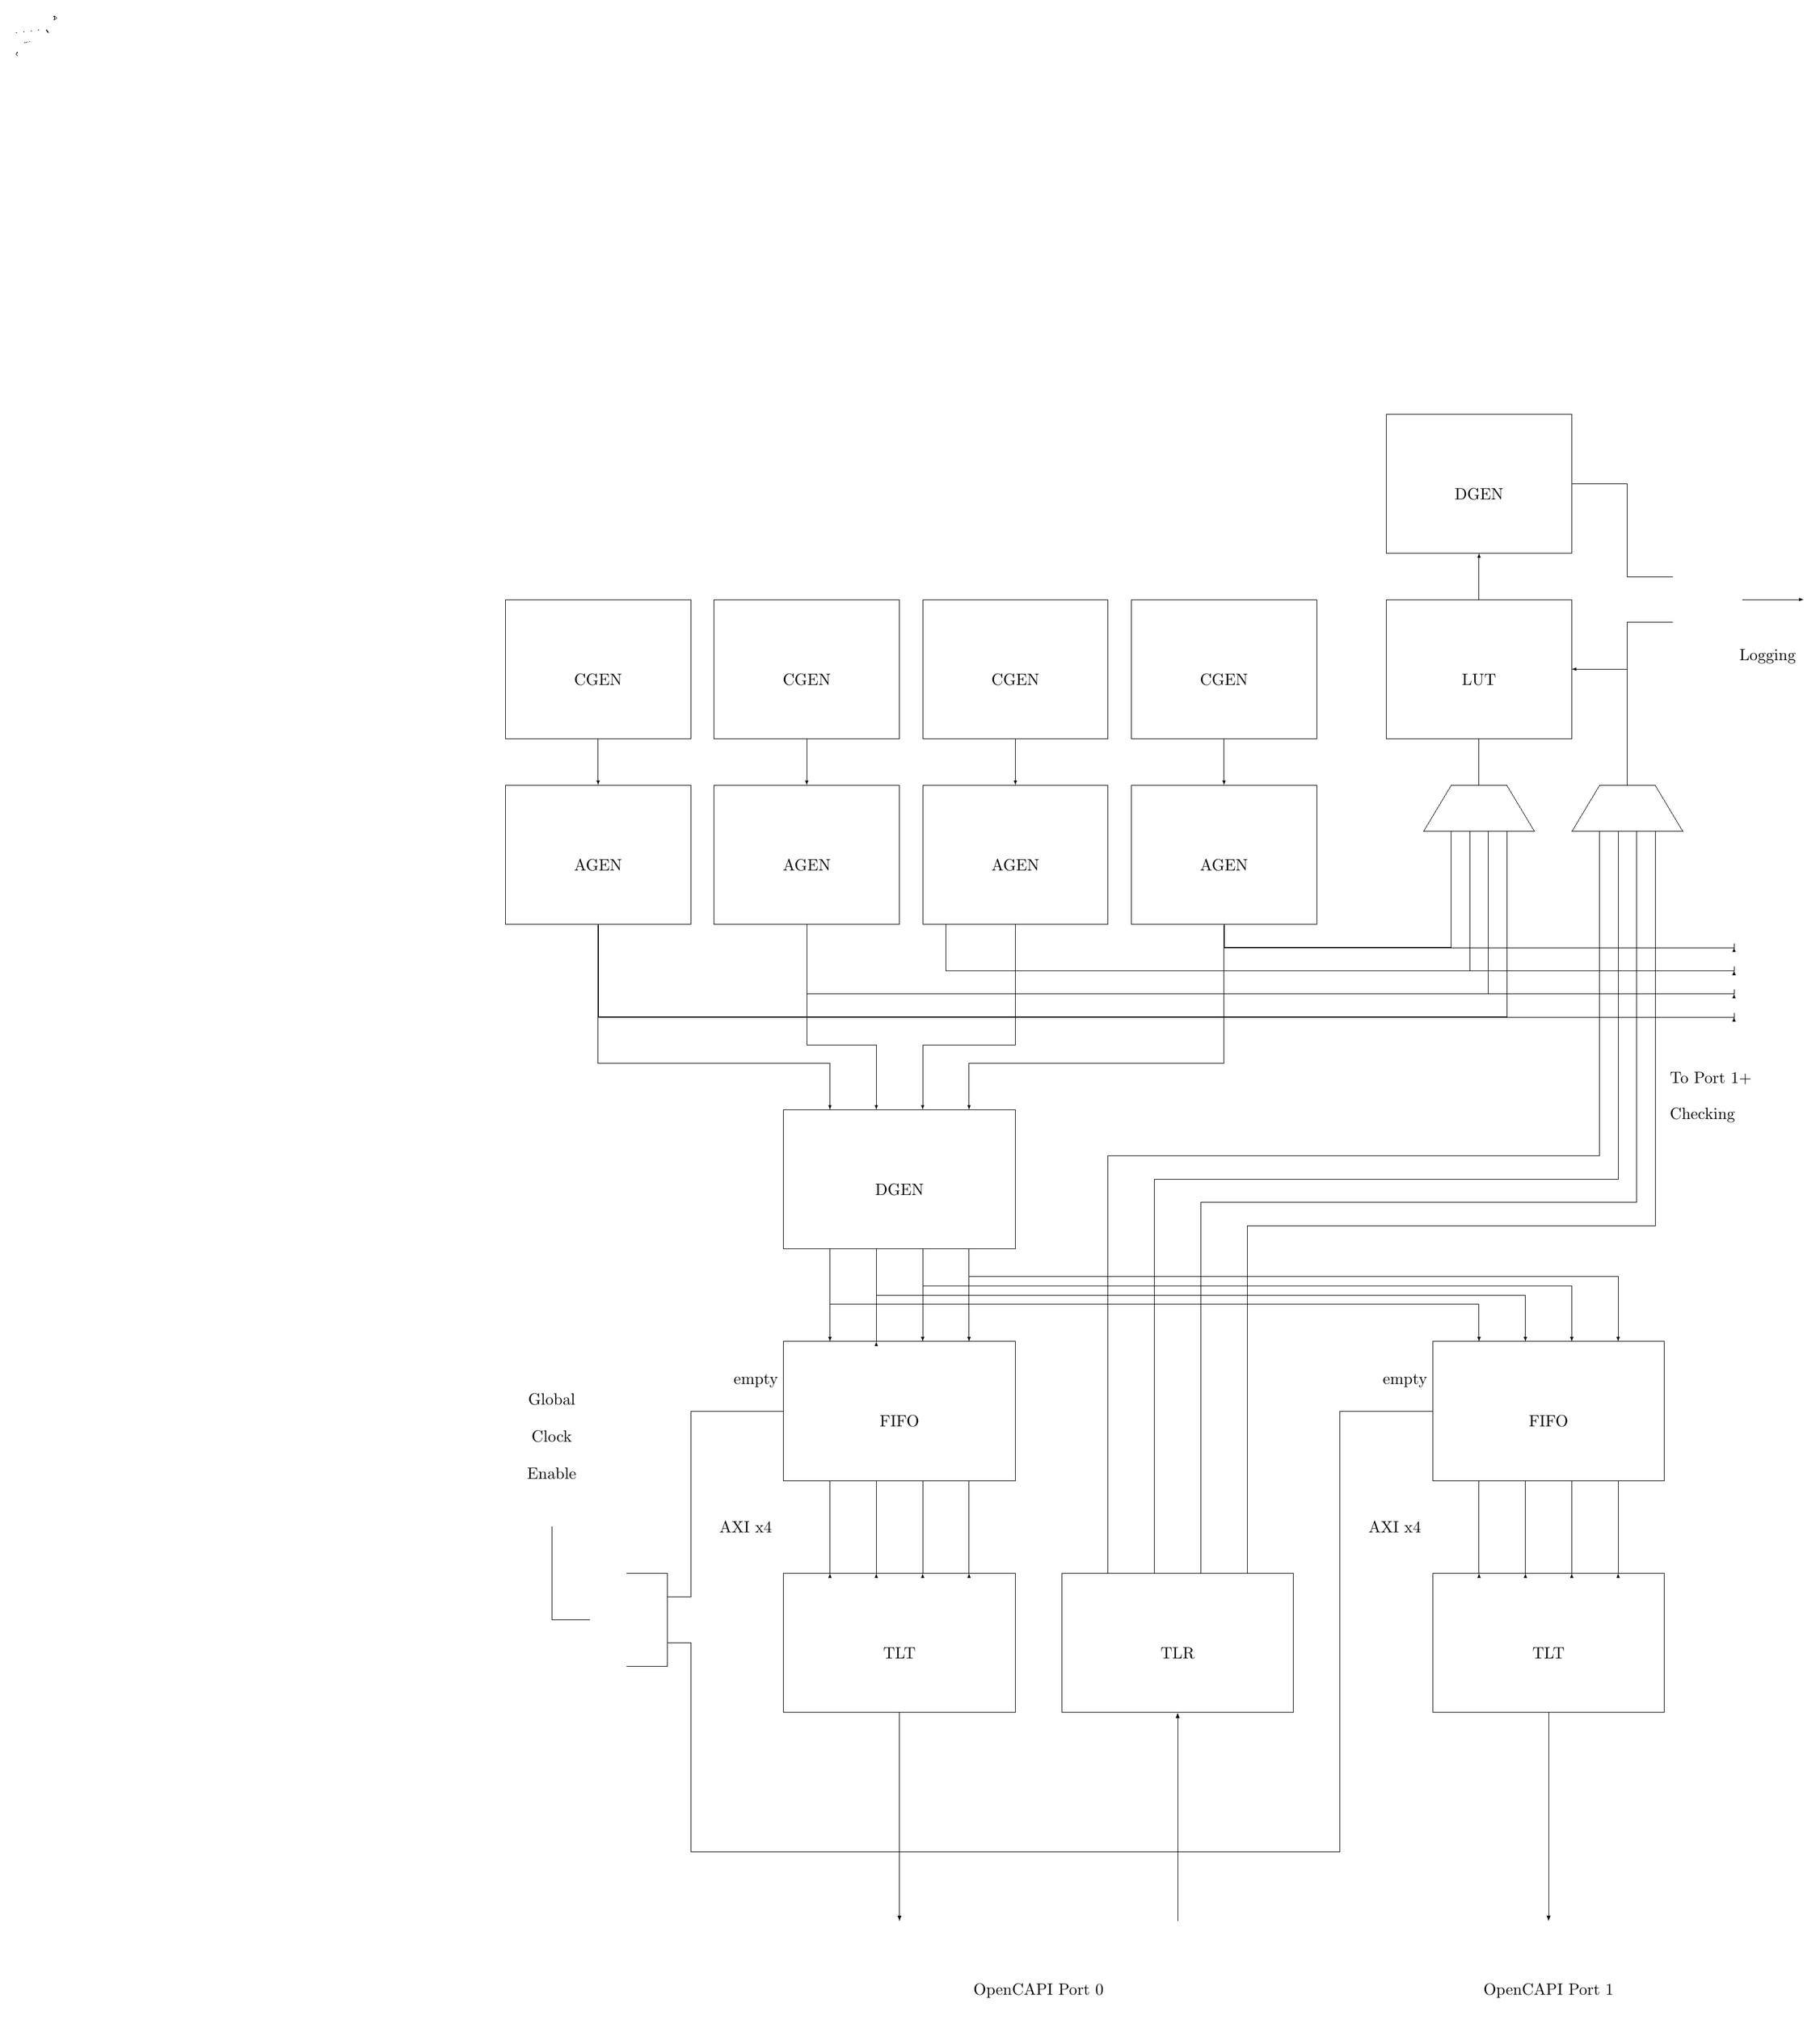
\begin{tikzpicture}
\pgftransformxscale{1.000000}
\pgftransformyscale{-1.000000}
\definecolor{dialinecolor}{rgb}{0.000000, 0.000000, 0.000000}
\pgfsetstrokecolor{dialinecolor}
\definecolor{dialinecolor}{rgb}{1.000000, 1.000000, 1.000000}
\pgfsetfillcolor{dialinecolor}
\pgfsetlinewidth{0.000000\du}
\pgfsetdash{}{0pt}
\pgfsetdash{}{0pt}
\pgfsetmiterjoin
\definecolor{dialinecolor}{rgb}{1.000000, 1.000000, 1.000000}
\pgfsetfillcolor{dialinecolor}
\fill (11.000000\du,13.000000\du)--(11.000000\du,16.000000\du)--(15.000000\du,16.000000\du)--(15.000000\du,13.000000\du)--cycle;
\definecolor{dialinecolor}{rgb}{0.000000, 0.000000, 0.000000}
\pgfsetstrokecolor{dialinecolor}
\draw (11.000000\du,13.000000\du)--(11.000000\du,16.000000\du)--(15.000000\du,16.000000\du)--(15.000000\du,13.000000\du)--cycle;
% setfont left to latex
\definecolor{dialinecolor}{rgb}{0.000000, 0.000000, 0.000000}
\pgfsetstrokecolor{dialinecolor}
\node at (13.000000\du,14.721250\du){CGEN};
\pgfsetlinewidth{0.000000\du}
\pgfsetdash{}{0pt}
\pgfsetdash{}{0pt}
\pgfsetmiterjoin
\definecolor{dialinecolor}{rgb}{1.000000, 1.000000, 1.000000}
\pgfsetfillcolor{dialinecolor}
\fill (11.000000\du,17.000000\du)--(11.000000\du,20.000000\du)--(15.000000\du,20.000000\du)--(15.000000\du,17.000000\du)--cycle;
\definecolor{dialinecolor}{rgb}{0.000000, 0.000000, 0.000000}
\pgfsetstrokecolor{dialinecolor}
\draw (11.000000\du,17.000000\du)--(11.000000\du,20.000000\du)--(15.000000\du,20.000000\du)--(15.000000\du,17.000000\du)--cycle;
% setfont left to latex
\definecolor{dialinecolor}{rgb}{0.000000, 0.000000, 0.000000}
\pgfsetstrokecolor{dialinecolor}
\node at (13.000000\du,18.721250\du){AGEN};
\pgfsetlinewidth{0.000000\du}
\pgfsetdash{}{0pt}
\pgfsetdash{}{0pt}
\pgfsetbuttcap
{
\definecolor{dialinecolor}{rgb}{0.000000, 0.000000, 0.000000}
\pgfsetfillcolor{dialinecolor}
% was here!!!
\pgfsetarrowsend{latex}
\definecolor{dialinecolor}{rgb}{0.000000, 0.000000, 0.000000}
\pgfsetstrokecolor{dialinecolor}
\draw (13.000000\du,16.000000\du)--(13.000000\du,17.000000\du);
}
\pgfsetlinewidth{0.000000\du}
\pgfsetdash{}{0pt}
\pgfsetdash{}{0pt}
\pgfsetmiterjoin
\definecolor{dialinecolor}{rgb}{1.000000, 1.000000, 1.000000}
\pgfsetfillcolor{dialinecolor}
\fill (15.500000\du,13.000000\du)--(15.500000\du,16.000000\du)--(19.500000\du,16.000000\du)--(19.500000\du,13.000000\du)--cycle;
\definecolor{dialinecolor}{rgb}{0.000000, 0.000000, 0.000000}
\pgfsetstrokecolor{dialinecolor}
\draw (15.500000\du,13.000000\du)--(15.500000\du,16.000000\du)--(19.500000\du,16.000000\du)--(19.500000\du,13.000000\du)--cycle;
% setfont left to latex
\definecolor{dialinecolor}{rgb}{0.000000, 0.000000, 0.000000}
\pgfsetstrokecolor{dialinecolor}
\node at (17.500000\du,14.721250\du){CGEN};
\pgfsetlinewidth{0.000000\du}
\pgfsetdash{}{0pt}
\pgfsetdash{}{0pt}
\pgfsetmiterjoin
\definecolor{dialinecolor}{rgb}{1.000000, 1.000000, 1.000000}
\pgfsetfillcolor{dialinecolor}
\fill (15.500000\du,17.000000\du)--(15.500000\du,20.000000\du)--(19.500000\du,20.000000\du)--(19.500000\du,17.000000\du)--cycle;
\definecolor{dialinecolor}{rgb}{0.000000, 0.000000, 0.000000}
\pgfsetstrokecolor{dialinecolor}
\draw (15.500000\du,17.000000\du)--(15.500000\du,20.000000\du)--(19.500000\du,20.000000\du)--(19.500000\du,17.000000\du)--cycle;
% setfont left to latex
\definecolor{dialinecolor}{rgb}{0.000000, 0.000000, 0.000000}
\pgfsetstrokecolor{dialinecolor}
\node at (17.500000\du,18.721250\du){AGEN};
\pgfsetlinewidth{0.000000\du}
\pgfsetdash{}{0pt}
\pgfsetdash{}{0pt}
\pgfsetbuttcap
{
\definecolor{dialinecolor}{rgb}{0.000000, 0.000000, 0.000000}
\pgfsetfillcolor{dialinecolor}
% was here!!!
\pgfsetarrowsend{latex}
\definecolor{dialinecolor}{rgb}{0.000000, 0.000000, 0.000000}
\pgfsetstrokecolor{dialinecolor}
\draw (17.500000\du,16.000000\du)--(17.500000\du,17.000000\du);
}
\pgfsetlinewidth{0.000000\du}
\pgfsetdash{}{0pt}
\pgfsetdash{}{0pt}
\pgfsetmiterjoin
\definecolor{dialinecolor}{rgb}{1.000000, 1.000000, 1.000000}
\pgfsetfillcolor{dialinecolor}
\fill (20.000000\du,13.000000\du)--(20.000000\du,16.000000\du)--(24.000000\du,16.000000\du)--(24.000000\du,13.000000\du)--cycle;
\definecolor{dialinecolor}{rgb}{0.000000, 0.000000, 0.000000}
\pgfsetstrokecolor{dialinecolor}
\draw (20.000000\du,13.000000\du)--(20.000000\du,16.000000\du)--(24.000000\du,16.000000\du)--(24.000000\du,13.000000\du)--cycle;
% setfont left to latex
\definecolor{dialinecolor}{rgb}{0.000000, 0.000000, 0.000000}
\pgfsetstrokecolor{dialinecolor}
\node at (22.000000\du,14.721250\du){CGEN};
\pgfsetlinewidth{0.000000\du}
\pgfsetdash{}{0pt}
\pgfsetdash{}{0pt}
\pgfsetmiterjoin
\definecolor{dialinecolor}{rgb}{1.000000, 1.000000, 1.000000}
\pgfsetfillcolor{dialinecolor}
\fill (20.000000\du,17.000000\du)--(20.000000\du,20.000000\du)--(24.000000\du,20.000000\du)--(24.000000\du,17.000000\du)--cycle;
\definecolor{dialinecolor}{rgb}{0.000000, 0.000000, 0.000000}
\pgfsetstrokecolor{dialinecolor}
\draw (20.000000\du,17.000000\du)--(20.000000\du,20.000000\du)--(24.000000\du,20.000000\du)--(24.000000\du,17.000000\du)--cycle;
% setfont left to latex
\definecolor{dialinecolor}{rgb}{0.000000, 0.000000, 0.000000}
\pgfsetstrokecolor{dialinecolor}
\node at (22.000000\du,18.721250\du){AGEN};
\pgfsetlinewidth{0.000000\du}
\pgfsetdash{}{0pt}
\pgfsetdash{}{0pt}
\pgfsetbuttcap
{
\definecolor{dialinecolor}{rgb}{0.000000, 0.000000, 0.000000}
\pgfsetfillcolor{dialinecolor}
% was here!!!
\pgfsetarrowsend{latex}
\definecolor{dialinecolor}{rgb}{0.000000, 0.000000, 0.000000}
\pgfsetstrokecolor{dialinecolor}
\draw (22.000000\du,16.000000\du)--(22.000000\du,17.000000\du);
}
\pgfsetlinewidth{0.000000\du}
\pgfsetdash{}{0pt}
\pgfsetdash{}{0pt}
\pgfsetmiterjoin
\definecolor{dialinecolor}{rgb}{1.000000, 1.000000, 1.000000}
\pgfsetfillcolor{dialinecolor}
\fill (24.500000\du,13.000000\du)--(24.500000\du,16.000000\du)--(28.500000\du,16.000000\du)--(28.500000\du,13.000000\du)--cycle;
\definecolor{dialinecolor}{rgb}{0.000000, 0.000000, 0.000000}
\pgfsetstrokecolor{dialinecolor}
\draw (24.500000\du,13.000000\du)--(24.500000\du,16.000000\du)--(28.500000\du,16.000000\du)--(28.500000\du,13.000000\du)--cycle;
% setfont left to latex
\definecolor{dialinecolor}{rgb}{0.000000, 0.000000, 0.000000}
\pgfsetstrokecolor{dialinecolor}
\node at (26.500000\du,14.721250\du){CGEN};
\pgfsetlinewidth{0.000000\du}
\pgfsetdash{}{0pt}
\pgfsetdash{}{0pt}
\pgfsetmiterjoin
\definecolor{dialinecolor}{rgb}{1.000000, 1.000000, 1.000000}
\pgfsetfillcolor{dialinecolor}
\fill (24.500000\du,17.000000\du)--(24.500000\du,20.000000\du)--(28.500000\du,20.000000\du)--(28.500000\du,17.000000\du)--cycle;
\definecolor{dialinecolor}{rgb}{0.000000, 0.000000, 0.000000}
\pgfsetstrokecolor{dialinecolor}
\draw (24.500000\du,17.000000\du)--(24.500000\du,20.000000\du)--(28.500000\du,20.000000\du)--(28.500000\du,17.000000\du)--cycle;
% setfont left to latex
\definecolor{dialinecolor}{rgb}{0.000000, 0.000000, 0.000000}
\pgfsetstrokecolor{dialinecolor}
\node at (26.500000\du,18.721250\du){AGEN};
\pgfsetlinewidth{0.000000\du}
\pgfsetdash{}{0pt}
\pgfsetdash{}{0pt}
\pgfsetbuttcap
{
\definecolor{dialinecolor}{rgb}{0.000000, 0.000000, 0.000000}
\pgfsetfillcolor{dialinecolor}
% was here!!!
\pgfsetarrowsend{latex}
\definecolor{dialinecolor}{rgb}{0.000000, 0.000000, 0.000000}
\pgfsetstrokecolor{dialinecolor}
\draw (26.500000\du,16.000000\du)--(26.500000\du,17.000000\du);
}
\pgfsetlinewidth{0.000000\du}
\pgfsetdash{}{0pt}
\pgfsetdash{}{0pt}
\pgfsetmiterjoin
\definecolor{dialinecolor}{rgb}{1.000000, 1.000000, 1.000000}
\pgfsetfillcolor{dialinecolor}
\fill (30.000000\du,13.000000\du)--(30.000000\du,16.000000\du)--(34.000000\du,16.000000\du)--(34.000000\du,13.000000\du)--cycle;
\definecolor{dialinecolor}{rgb}{0.000000, 0.000000, 0.000000}
\pgfsetstrokecolor{dialinecolor}
\draw (30.000000\du,13.000000\du)--(30.000000\du,16.000000\du)--(34.000000\du,16.000000\du)--(34.000000\du,13.000000\du)--cycle;
% setfont left to latex
\definecolor{dialinecolor}{rgb}{0.000000, 0.000000, 0.000000}
\pgfsetstrokecolor{dialinecolor}
\node at (32.000000\du,14.721250\du){LUT};
\pgfsetlinewidth{0.000000\du}
\pgfsetdash{}{0pt}
\pgfsetdash{}{0pt}
\pgfsetmiterjoin
\definecolor{dialinecolor}{rgb}{1.000000, 1.000000, 1.000000}
\pgfsetfillcolor{dialinecolor}
\fill (17.000000\du,24.000000\du)--(17.000000\du,27.000000\du)--(22.000000\du,27.000000\du)--(22.000000\du,24.000000\du)--cycle;
\definecolor{dialinecolor}{rgb}{0.000000, 0.000000, 0.000000}
\pgfsetstrokecolor{dialinecolor}
\draw (17.000000\du,24.000000\du)--(17.000000\du,27.000000\du)--(22.000000\du,27.000000\du)--(22.000000\du,24.000000\du)--cycle;
% setfont left to latex
\definecolor{dialinecolor}{rgb}{0.000000, 0.000000, 0.000000}
\pgfsetstrokecolor{dialinecolor}
\node at (19.500000\du,25.721250\du){DGEN};
\pgfsetlinewidth{0.000000\du}
\pgfsetdash{}{0pt}
\pgfsetdash{}{0pt}
\pgfsetmiterjoin
\pgfsetbuttcap
{
\definecolor{dialinecolor}{rgb}{0.000000, 0.000000, 0.000000}
\pgfsetfillcolor{dialinecolor}
% was here!!!
\pgfsetarrowsend{latex}
{\pgfsetcornersarced{\pgfpoint{0.000000\du}{0.000000\du}}\definecolor{dialinecolor}{rgb}{0.000000, 0.000000, 0.000000}
\pgfsetstrokecolor{dialinecolor}
\draw (13.000000\du,20.000000\du)--(13.000000\du,23.000000\du)--(18.000000\du,23.000000\du)--(18.000000\du,24.000000\du);
}}
\pgfsetlinewidth{0.000000\du}
\pgfsetdash{}{0pt}
\pgfsetdash{}{0pt}
\pgfsetmiterjoin
\pgfsetbuttcap
{
\definecolor{dialinecolor}{rgb}{0.000000, 0.000000, 0.000000}
\pgfsetfillcolor{dialinecolor}
% was here!!!
\pgfsetarrowsend{latex}
{\pgfsetcornersarced{\pgfpoint{0.000000\du}{0.000000\du}}\definecolor{dialinecolor}{rgb}{0.000000, 0.000000, 0.000000}
\pgfsetstrokecolor{dialinecolor}
\draw (17.500000\du,20.000000\du)--(17.500000\du,22.600000\du)--(19.000000\du,22.600000\du)--(19.000000\du,24.000000\du);
}}
\pgfsetlinewidth{0.000000\du}
\pgfsetdash{}{0pt}
\pgfsetdash{}{0pt}
\pgfsetmiterjoin
\pgfsetbuttcap
{
\definecolor{dialinecolor}{rgb}{0.000000, 0.000000, 0.000000}
\pgfsetfillcolor{dialinecolor}
% was here!!!
\pgfsetarrowsend{latex}
{\pgfsetcornersarced{\pgfpoint{0.000000\du}{0.000000\du}}\definecolor{dialinecolor}{rgb}{0.000000, 0.000000, 0.000000}
\pgfsetstrokecolor{dialinecolor}
\draw (22.000000\du,20.000000\du)--(22.000000\du,22.600000\du)--(20.000000\du,22.600000\du)--(20.000000\du,24.000000\du);
}}
\pgfsetlinewidth{0.000000\du}
\pgfsetdash{}{0pt}
\pgfsetdash{}{0pt}
\pgfsetmiterjoin
\pgfsetbuttcap
{
\definecolor{dialinecolor}{rgb}{0.000000, 0.000000, 0.000000}
\pgfsetfillcolor{dialinecolor}
% was here!!!
\pgfsetarrowsend{latex}
{\pgfsetcornersarced{\pgfpoint{0.000000\du}{0.000000\du}}\definecolor{dialinecolor}{rgb}{0.000000, 0.000000, 0.000000}
\pgfsetstrokecolor{dialinecolor}
\draw (26.500000\du,20.000000\du)--(26.500000\du,23.000000\du)--(21.000000\du,23.000000\du)--(21.000000\du,24.000000\du);
}}
\pgfsetlinewidth{0.000000\du}
\pgfsetdash{}{0pt}
\pgfsetdash{}{0pt}
\pgfsetbuttcap
{
\definecolor{dialinecolor}{rgb}{0.000000, 0.000000, 0.000000}
\pgfsetfillcolor{dialinecolor}
% was here!!!
\definecolor{dialinecolor}{rgb}{0.000000, 0.000000, 0.000000}
\pgfsetstrokecolor{dialinecolor}
\draw (17.000000\du,24.000000\du)--(22.000000\du,24.000000\du);
}
\pgfsetlinewidth{0.000000\du}
\pgfsetdash{}{0pt}
\pgfsetdash{}{0pt}
\pgfsetmiterjoin
\definecolor{dialinecolor}{rgb}{1.000000, 1.000000, 1.000000}
\pgfsetfillcolor{dialinecolor}
\fill (30.000000\du,9.000000\du)--(30.000000\du,12.000000\du)--(34.000000\du,12.000000\du)--(34.000000\du,9.000000\du)--cycle;
\definecolor{dialinecolor}{rgb}{0.000000, 0.000000, 0.000000}
\pgfsetstrokecolor{dialinecolor}
\draw (30.000000\du,9.000000\du)--(30.000000\du,12.000000\du)--(34.000000\du,12.000000\du)--(34.000000\du,9.000000\du)--cycle;
% setfont left to latex
\definecolor{dialinecolor}{rgb}{0.000000, 0.000000, 0.000000}
\pgfsetstrokecolor{dialinecolor}
\node at (32.000000\du,10.721250\du){DGEN};
\pgfsetlinewidth{0.000000\du}
\pgfsetdash{}{0pt}
\pgfsetdash{}{0pt}
\pgfsetbuttcap
\pgfsetmiterjoin
\pgfsetlinewidth{0.000000\du}
\pgfsetbuttcap
\pgfsetmiterjoin
\pgfsetdash{}{0pt}
\definecolor{dialinecolor}{rgb}{0.000000, 0.000000, 0.000000}
\pgfsetstrokecolor{dialinecolor}
\draw (30.800000\du,18.000000\du)--(33.200000\du,18.000000\du)--(32.600000\du,17.000000\du)--(31.400000\du,17.000000\du)--cycle;
% setfont left to latex
\definecolor{dialinecolor}{rgb}{0.000000, 0.000000, 0.000000}
\pgfsetstrokecolor{dialinecolor}
\node at (32.000000\du,17.700000\du){};
\pgfsetlinewidth{0.000000\du}
\pgfsetdash{}{0pt}
\pgfsetdash{}{0pt}
\pgfsetbuttcap
{
\definecolor{dialinecolor}{rgb}{0.000000, 0.000000, 0.000000}
\pgfsetfillcolor{dialinecolor}
% was here!!!
\definecolor{dialinecolor}{rgb}{0.000000, 0.000000, 0.000000}
\pgfsetstrokecolor{dialinecolor}
\draw (31.400000\du,18.000000\du)--(32.600000\du,18.000000\du);
}
\pgfsetlinewidth{0.000000\du}
\pgfsetdash{}{0pt}
\pgfsetdash{}{0pt}
\pgfsetbuttcap
{
\definecolor{dialinecolor}{rgb}{0.000000, 0.000000, 0.000000}
\pgfsetfillcolor{dialinecolor}
% was here!!!
\definecolor{dialinecolor}{rgb}{0.000000, 0.000000, 0.000000}
\pgfsetstrokecolor{dialinecolor}
\draw (32.000000\du,17.000000\du)--(32.000000\du,16.000000\du);
}
\pgfsetlinewidth{0.000000\du}
\pgfsetdash{}{0pt}
\pgfsetdash{}{0pt}
\pgfsetbuttcap
{
\definecolor{dialinecolor}{rgb}{0.000000, 0.000000, 0.000000}
\pgfsetfillcolor{dialinecolor}
% was here!!!
\pgfsetarrowsend{latex}
\definecolor{dialinecolor}{rgb}{0.000000, 0.000000, 0.000000}
\pgfsetstrokecolor{dialinecolor}
\draw (32.000000\du,13.000000\du)--(32.000000\du,12.000000\du);
}
\pgfsetlinewidth{0.000000\du}
\pgfsetdash{}{0pt}
\pgfsetdash{}{0pt}
\pgfsetmiterjoin
\pgfsetbuttcap
{
\definecolor{dialinecolor}{rgb}{0.000000, 0.000000, 0.000000}
\pgfsetfillcolor{dialinecolor}
% was here!!!
{\pgfsetcornersarced{\pgfpoint{0.000000\du}{0.000000\du}}\definecolor{dialinecolor}{rgb}{0.000000, 0.000000, 0.000000}
\pgfsetstrokecolor{dialinecolor}
\draw (31.400000\du,18.000000\du)--(31.400000\du,20.500000\du)--(26.500000\du,20.500000\du)--(26.500000\du,20.000000\du);
}}
\pgfsetlinewidth{0.000000\du}
\pgfsetdash{}{0pt}
\pgfsetdash{}{0pt}
\pgfsetmiterjoin
\pgfsetbuttcap
{
\definecolor{dialinecolor}{rgb}{0.000000, 0.000000, 0.000000}
\pgfsetfillcolor{dialinecolor}
% was here!!!
{\pgfsetcornersarced{\pgfpoint{0.000000\du}{0.000000\du}}\definecolor{dialinecolor}{rgb}{0.000000, 0.000000, 0.000000}
\pgfsetstrokecolor{dialinecolor}
\draw (31.800000\du,18.000000\du)--(31.800000\du,21.000000\du)--(22.000000\du,21.000000\du)--(22.000000\du,20.000000\du);
}}
\pgfsetlinewidth{0.000000\du}
\pgfsetdash{}{0pt}
\pgfsetdash{}{0pt}
\pgfsetmiterjoin
\pgfsetbuttcap
{
\definecolor{dialinecolor}{rgb}{0.000000, 0.000000, 0.000000}
\pgfsetfillcolor{dialinecolor}
% was here!!!
{\pgfsetcornersarced{\pgfpoint{0.000000\du}{0.000000\du}}\definecolor{dialinecolor}{rgb}{0.000000, 0.000000, 0.000000}
\pgfsetstrokecolor{dialinecolor}
\draw (32.200000\du,18.000000\du)--(32.200000\du,21.500000\du)--(17.500000\du,21.500000\du)--(17.500000\du,20.000000\du);
}}
\pgfsetlinewidth{0.000000\du}
\pgfsetdash{}{0pt}
\pgfsetdash{}{0pt}
\pgfsetmiterjoin
\pgfsetbuttcap
{
\definecolor{dialinecolor}{rgb}{0.000000, 0.000000, 0.000000}
\pgfsetfillcolor{dialinecolor}
% was here!!!
{\pgfsetcornersarced{\pgfpoint{0.000000\du}{0.000000\du}}\definecolor{dialinecolor}{rgb}{0.000000, 0.000000, 0.000000}
\pgfsetstrokecolor{dialinecolor}
\draw (32.600000\du,18.000000\du)--(32.600000\du,22.000000\du)--(13.000000\du,22.000000\du)--(13.000000\du,20.000000\du);
}}
\pgfsetlinewidth{0.000000\du}
\pgfsetdash{}{0pt}
\pgfsetdash{}{0pt}
\pgfsetbuttcap
\pgfsetmiterjoin
\pgfsetlinewidth{0.000000\du}
\pgfsetbuttcap
\pgfsetmiterjoin
\pgfsetdash{}{0pt}
\pgfsetbuttcap
\pgfsetmiterjoin
\pgfsetdash{}{0pt}
\definecolor{dialinecolor}{rgb}{0.000000, 0.000000, 0.000000}
\pgfsetfillcolor{dialinecolor}
\pgfpathellipse{\pgfpoint{13.000000\du}{22.000000\du}}{\pgfpoint{0.125000\du}{0\du}}{\pgfpoint{0\du}{0.125000\du}}
\pgfusepath{fill}
\definecolor{dialinecolor}{rgb}{0.000000, 0.000000, 0.000000}
\pgfsetstrokecolor{dialinecolor}
\pgfpathellipse{\pgfpoint{13.000000\du}{22.000000\du}}{\pgfpoint{0.125000\du}{0\du}}{\pgfpoint{0\du}{0.125000\du}}
\pgfusepath{stroke}
\pgfsetlinewidth{0.000000\du}
\pgfsetdash{}{0pt}
\pgfsetdash{}{0pt}
\pgfsetbuttcap
\pgfsetmiterjoin
\pgfsetlinewidth{0.000000\du}
\pgfsetbuttcap
\pgfsetmiterjoin
\pgfsetdash{}{0pt}
\pgfsetbuttcap
\pgfsetmiterjoin
\pgfsetdash{}{0pt}
\definecolor{dialinecolor}{rgb}{0.000000, 0.000000, 0.000000}
\pgfsetfillcolor{dialinecolor}
\pgfpathellipse{\pgfpoint{17.500000\du}{21.500000\du}}{\pgfpoint{0.125000\du}{0\du}}{\pgfpoint{0\du}{0.125000\du}}
\pgfusepath{fill}
\definecolor{dialinecolor}{rgb}{0.000000, 0.000000, 0.000000}
\pgfsetstrokecolor{dialinecolor}
\pgfpathellipse{\pgfpoint{17.500000\du}{21.500000\du}}{\pgfpoint{0.125000\du}{0\du}}{\pgfpoint{0\du}{0.125000\du}}
\pgfusepath{stroke}
\pgfsetlinewidth{0.000000\du}
\pgfsetdash{}{0pt}
\pgfsetdash{}{0pt}
\pgfsetbuttcap
\pgfsetmiterjoin
\pgfsetlinewidth{0.000000\du}
\pgfsetbuttcap
\pgfsetmiterjoin
\pgfsetdash{}{0pt}
\pgfsetbuttcap
\pgfsetmiterjoin
\pgfsetdash{}{0pt}
\definecolor{dialinecolor}{rgb}{0.000000, 0.000000, 0.000000}
\pgfsetfillcolor{dialinecolor}
\pgfpathellipse{\pgfpoint{22.000000\du}{21.000000\du}}{\pgfpoint{0.125000\du}{0\du}}{\pgfpoint{0\du}{0.125000\du}}
\pgfusepath{fill}
\definecolor{dialinecolor}{rgb}{0.000000, 0.000000, 0.000000}
\pgfsetstrokecolor{dialinecolor}
\pgfpathellipse{\pgfpoint{22.000000\du}{21.000000\du}}{\pgfpoint{0.125000\du}{0\du}}{\pgfpoint{0\du}{0.125000\du}}
\pgfusepath{stroke}
\pgfsetlinewidth{0.000000\du}
\pgfsetdash{}{0pt}
\pgfsetdash{}{0pt}
\pgfsetbuttcap
\pgfsetmiterjoin
\pgfsetlinewidth{0.000000\du}
\pgfsetbuttcap
\pgfsetmiterjoin
\pgfsetdash{}{0pt}
\pgfsetbuttcap
\pgfsetmiterjoin
\pgfsetdash{}{0pt}
\definecolor{dialinecolor}{rgb}{0.000000, 0.000000, 0.000000}
\pgfsetfillcolor{dialinecolor}
\pgfpathellipse{\pgfpoint{26.500000\du}{20.500000\du}}{\pgfpoint{0.125000\du}{0\du}}{\pgfpoint{0\du}{0.125000\du}}
\pgfusepath{fill}
\definecolor{dialinecolor}{rgb}{0.000000, 0.000000, 0.000000}
\pgfsetstrokecolor{dialinecolor}
\pgfpathellipse{\pgfpoint{26.500000\du}{20.500000\du}}{\pgfpoint{0.125000\du}{0\du}}{\pgfpoint{0\du}{0.125000\du}}
\pgfusepath{stroke}
\pgfsetlinewidth{0.000000\du}
\pgfsetdash{}{0pt}
\pgfsetdash{}{0pt}
\pgfsetbuttcap
\pgfsetmiterjoin
\pgfsetlinewidth{0.000000\du}
\pgfsetbuttcap
\pgfsetmiterjoin
\pgfsetdash{}{0pt}
\definecolor{dialinecolor}{rgb}{0.000000, 0.000000, 0.000000}
\pgfsetstrokecolor{dialinecolor}
\pgfpathmoveto{\pgfpoint{37.680000\du}{13.000000\du}}
\pgfpathcurveto{\pgfpoint{37.311059\du}{12.367961\du}}{\pgfpoint{36.712569\du}{12.000000\du}}{\pgfpoint{36.080000\du}{12.016294\du}}
\pgfusepath{stroke}
\pgfsetbuttcap
\pgfsetmiterjoin
\pgfsetdash{}{0pt}
\definecolor{dialinecolor}{rgb}{0.000000, 0.000000, 0.000000}
\pgfsetstrokecolor{dialinecolor}
\pgfpathmoveto{\pgfpoint{36.080000\du}{13.983706\du}}
\pgfpathcurveto{\pgfpoint{36.712569\du}{14.000000\du}}{\pgfpoint{37.311059\du}{13.632039\du}}{\pgfpoint{37.680000\du}{13.000000\du}}
\pgfusepath{stroke}
\pgfsetbuttcap
\pgfsetmiterjoin
\pgfsetdash{}{0pt}
\definecolor{dialinecolor}{rgb}{0.000000, 0.000000, 0.000000}
\pgfsetstrokecolor{dialinecolor}
\pgfpathmoveto{\pgfpoint{36.000000\du}{13.983706\du}}
\pgfpathcurveto{\pgfpoint{36.320000\du}{13.386925\du}}{\pgfpoint{36.320000\du}{12.613075\du}}{\pgfpoint{36.000000\du}{12.016294\du}}
\pgfusepath{stroke}
\pgfsetbuttcap
\pgfsetmiterjoin
\pgfsetdash{}{0pt}
\definecolor{dialinecolor}{rgb}{0.000000, 0.000000, 0.000000}
\pgfsetstrokecolor{dialinecolor}
\draw (37.680000\du,13.000000\du)--(38.000000\du,13.000000\du);
\pgfsetbuttcap
\pgfsetmiterjoin
\pgfsetdash{}{0pt}
\definecolor{dialinecolor}{rgb}{0.000000, 0.000000, 0.000000}
\pgfsetstrokecolor{dialinecolor}
\pgfpathmoveto{\pgfpoint{36.080000\du}{13.983706\du}}
\pgfpathcurveto{\pgfpoint{36.400000\du}{13.386925\du}}{\pgfpoint{36.400000\du}{12.613075\du}}{\pgfpoint{36.080000\du}{12.016294\du}}
\pgfusepath{stroke}
\pgfsetlinewidth{0.000000\du}
\pgfsetdash{}{0pt}
\pgfsetdash{}{0pt}
\pgfsetmiterjoin
\pgfsetbuttcap
{
\definecolor{dialinecolor}{rgb}{0.000000, 0.000000, 0.000000}
\pgfsetfillcolor{dialinecolor}
% was here!!!
{\pgfsetcornersarced{\pgfpoint{0.000000\du}{0.000000\du}}\definecolor{dialinecolor}{rgb}{0.000000, 0.000000, 0.000000}
\pgfsetstrokecolor{dialinecolor}
\draw (35.200000\du,17.000000\du)--(35.200000\du,17.000000\du)--(35.200000\du,13.491853\du)--(36.176000\du,13.491853\du);
}}
\pgfsetlinewidth{0.000000\du}
\pgfsetdash{}{0pt}
\pgfsetdash{}{0pt}
\pgfsetmiterjoin
\pgfsetbuttcap
{
\definecolor{dialinecolor}{rgb}{0.000000, 0.000000, 0.000000}
\pgfsetfillcolor{dialinecolor}
% was here!!!
{\pgfsetcornersarced{\pgfpoint{0.000000\du}{0.000000\du}}\definecolor{dialinecolor}{rgb}{0.000000, 0.000000, 0.000000}
\pgfsetstrokecolor{dialinecolor}
\draw (34.000000\du,10.500000\du)--(35.200000\du,10.500000\du)--(35.200000\du,12.508147\du)--(36.176000\du,12.508147\du);
}}
\pgfsetlinewidth{0.000000\du}
\pgfsetdash{}{0pt}
\pgfsetdash{}{0pt}
\pgfsetbuttcap
{
\definecolor{dialinecolor}{rgb}{0.000000, 0.000000, 0.000000}
\pgfsetfillcolor{dialinecolor}
% was here!!!
\pgfsetarrowsend{latex}
\definecolor{dialinecolor}{rgb}{0.000000, 0.000000, 0.000000}
\pgfsetstrokecolor{dialinecolor}
\draw (38.000000\du,13.000000\du)--(39.000000\du,13.000000\du);
}
% setfont left to latex
\definecolor{dialinecolor}{rgb}{0.000000, 0.000000, 0.000000}
\pgfsetstrokecolor{dialinecolor}
\node[anchor=west] at (37.500000\du,14.221250\du){ Logging};
\pgfsetlinewidth{0.000000\du}
\pgfsetdash{}{0pt}
\pgfsetdash{}{0pt}
\pgfsetmiterjoin
\definecolor{dialinecolor}{rgb}{1.000000, 1.000000, 1.000000}
\pgfsetfillcolor{dialinecolor}
\fill (17.000000\du,34.000000\du)--(17.000000\du,37.000000\du)--(22.000000\du,37.000000\du)--(22.000000\du,34.000000\du)--cycle;
\definecolor{dialinecolor}{rgb}{0.000000, 0.000000, 0.000000}
\pgfsetstrokecolor{dialinecolor}
\draw (17.000000\du,34.000000\du)--(17.000000\du,37.000000\du)--(22.000000\du,37.000000\du)--(22.000000\du,34.000000\du)--cycle;
% setfont left to latex
\definecolor{dialinecolor}{rgb}{0.000000, 0.000000, 0.000000}
\pgfsetstrokecolor{dialinecolor}
\node at (19.500000\du,35.721250\du){TLT};
\pgfsetlinewidth{0.000000\du}
\pgfsetdash{}{0pt}
\pgfsetdash{}{0pt}
\pgfsetmiterjoin
\definecolor{dialinecolor}{rgb}{1.000000, 1.000000, 1.000000}
\pgfsetfillcolor{dialinecolor}
\fill (23.000000\du,34.000000\du)--(23.000000\du,37.000000\du)--(28.000000\du,37.000000\du)--(28.000000\du,34.000000\du)--cycle;
\definecolor{dialinecolor}{rgb}{0.000000, 0.000000, 0.000000}
\pgfsetstrokecolor{dialinecolor}
\draw (23.000000\du,34.000000\du)--(23.000000\du,37.000000\du)--(28.000000\du,37.000000\du)--(28.000000\du,34.000000\du)--cycle;
% setfont left to latex
\definecolor{dialinecolor}{rgb}{0.000000, 0.000000, 0.000000}
\pgfsetstrokecolor{dialinecolor}
\node at (25.500000\du,35.721250\du){TLR};
\pgfsetlinewidth{0.000000\du}
\pgfsetdash{}{0pt}
\pgfsetdash{}{0pt}
\pgfsetmiterjoin
\definecolor{dialinecolor}{rgb}{1.000000, 1.000000, 1.000000}
\pgfsetfillcolor{dialinecolor}
\fill (17.000000\du,29.000000\du)--(17.000000\du,32.000000\du)--(22.000000\du,32.000000\du)--(22.000000\du,29.000000\du)--cycle;
\definecolor{dialinecolor}{rgb}{0.000000, 0.000000, 0.000000}
\pgfsetstrokecolor{dialinecolor}
\draw (17.000000\du,29.000000\du)--(17.000000\du,32.000000\du)--(22.000000\du,32.000000\du)--(22.000000\du,29.000000\du)--cycle;
% setfont left to latex
\definecolor{dialinecolor}{rgb}{0.000000, 0.000000, 0.000000}
\pgfsetstrokecolor{dialinecolor}
\node at (19.500000\du,30.721250\du){FIFO};
\pgfsetlinewidth{0.000000\du}
\pgfsetdash{}{0pt}
\pgfsetdash{}{0pt}
\pgfsetbuttcap
{
\definecolor{dialinecolor}{rgb}{0.000000, 0.000000, 0.000000}
\pgfsetfillcolor{dialinecolor}
% was here!!!
\definecolor{dialinecolor}{rgb}{0.000000, 0.000000, 0.000000}
\pgfsetstrokecolor{dialinecolor}
\draw (23.000000\du,34.000000\du)--(28.000000\du,34.000000\du);
}
\pgfsetlinewidth{0.000000\du}
\pgfsetdash{}{0pt}
\pgfsetdash{}{0pt}
\pgfsetmiterjoin
\pgfsetbuttcap
{
\definecolor{dialinecolor}{rgb}{0.000000, 0.000000, 0.000000}
\pgfsetfillcolor{dialinecolor}
% was here!!!
{\pgfsetcornersarced{\pgfpoint{0.000000\du}{0.000000\du}}\definecolor{dialinecolor}{rgb}{0.000000, 0.000000, 0.000000}
\pgfsetstrokecolor{dialinecolor}
\draw (24.000000\du,34.000000\du)--(24.000000\du,25.000000\du)--(34.600000\du,25.000000\du)--(34.600000\du,18.000000\du);
}}
\pgfsetlinewidth{0.000000\du}
\pgfsetdash{}{0pt}
\pgfsetdash{}{0pt}
\pgfsetmiterjoin
\pgfsetbuttcap
{
\definecolor{dialinecolor}{rgb}{0.000000, 0.000000, 0.000000}
\pgfsetfillcolor{dialinecolor}
% was here!!!
{\pgfsetcornersarced{\pgfpoint{0.000000\du}{0.000000\du}}\definecolor{dialinecolor}{rgb}{0.000000, 0.000000, 0.000000}
\pgfsetstrokecolor{dialinecolor}
\draw (25.000000\du,34.000000\du)--(25.000000\du,25.500000\du)--(35.000000\du,25.500000\du)--(35.000000\du,18.000000\du);
}}
\pgfsetlinewidth{0.000000\du}
\pgfsetdash{}{0pt}
\pgfsetdash{}{0pt}
\pgfsetmiterjoin
\pgfsetbuttcap
{
\definecolor{dialinecolor}{rgb}{0.000000, 0.000000, 0.000000}
\pgfsetfillcolor{dialinecolor}
% was here!!!
{\pgfsetcornersarced{\pgfpoint{0.000000\du}{0.000000\du}}\definecolor{dialinecolor}{rgb}{0.000000, 0.000000, 0.000000}
\pgfsetstrokecolor{dialinecolor}
\draw (26.000000\du,34.000000\du)--(26.000000\du,26.000000\du)--(35.400000\du,26.000000\du)--(35.400000\du,18.000000\du);
}}
\pgfsetlinewidth{0.000000\du}
\pgfsetdash{}{0pt}
\pgfsetdash{}{0pt}
\pgfsetmiterjoin
\pgfsetbuttcap
{
\definecolor{dialinecolor}{rgb}{0.000000, 0.000000, 0.000000}
\pgfsetfillcolor{dialinecolor}
% was here!!!
{\pgfsetcornersarced{\pgfpoint{0.000000\du}{0.000000\du}}\definecolor{dialinecolor}{rgb}{0.000000, 0.000000, 0.000000}
\pgfsetstrokecolor{dialinecolor}
\draw (27.000000\du,34.000000\du)--(27.000000\du,26.500000\du)--(35.800000\du,26.500000\du)--(35.800000\du,18.000000\du);
}}
\pgfsetlinewidth{0.000000\du}
\pgfsetdash{}{0pt}
\pgfsetdash{}{0pt}
\pgfsetbuttcap
{
\definecolor{dialinecolor}{rgb}{0.000000, 0.000000, 0.000000}
\pgfsetfillcolor{dialinecolor}
% was here!!!
\definecolor{dialinecolor}{rgb}{0.000000, 0.000000, 0.000000}
\pgfsetstrokecolor{dialinecolor}
\draw (17.000000\du,29.000000\du)--(22.000000\du,29.000000\du);
}
\pgfsetlinewidth{0.000000\du}
\pgfsetdash{}{0pt}
\pgfsetdash{}{0pt}
\pgfsetbuttcap
{
\definecolor{dialinecolor}{rgb}{0.000000, 0.000000, 0.000000}
\pgfsetfillcolor{dialinecolor}
% was here!!!
\definecolor{dialinecolor}{rgb}{0.000000, 0.000000, 0.000000}
\pgfsetstrokecolor{dialinecolor}
\draw (17.000000\du,27.000000\du)--(22.000000\du,27.000000\du);
}
\pgfsetlinewidth{0.000000\du}
\pgfsetdash{}{0pt}
\pgfsetdash{}{0pt}
\pgfsetmiterjoin
\pgfsetbuttcap
{
\definecolor{dialinecolor}{rgb}{0.000000, 0.000000, 0.000000}
\pgfsetfillcolor{dialinecolor}
% was here!!!
\pgfsetarrowsend{latex}
{\pgfsetcornersarced{\pgfpoint{0.000000\du}{0.000000\du}}\definecolor{dialinecolor}{rgb}{0.000000, 0.000000, 0.000000}
\pgfsetstrokecolor{dialinecolor}
\draw (18.000000\du,27.000000\du)--(18.000000\du,28.200000\du)--(18.000000\du,28.200000\du)--(18.000000\du,29.000000\du);
}}
\pgfsetlinewidth{0.000000\du}
\pgfsetdash{}{0pt}
\pgfsetdash{}{0pt}
\pgfsetmiterjoin
\pgfsetbuttcap
{
\definecolor{dialinecolor}{rgb}{0.000000, 0.000000, 0.000000}
\pgfsetfillcolor{dialinecolor}
% was here!!!
\pgfsetarrowsend{latex}
{\pgfsetcornersarced{\pgfpoint{0.000000\du}{0.000000\du}}\definecolor{dialinecolor}{rgb}{0.000000, 0.000000, 0.000000}
\pgfsetstrokecolor{dialinecolor}
\draw (19.000000\du,27.000000\du)--(19.000000\du,27.000000\du)--(19.000000\du,29.000000\du)--(19.000000\du,29.000000\du);
}}
\pgfsetlinewidth{0.000000\du}
\pgfsetdash{}{0pt}
\pgfsetdash{}{0pt}
\pgfsetmiterjoin
\pgfsetbuttcap
{
\definecolor{dialinecolor}{rgb}{0.000000, 0.000000, 0.000000}
\pgfsetfillcolor{dialinecolor}
% was here!!!
\pgfsetarrowsend{latex}
{\pgfsetcornersarced{\pgfpoint{0.000000\du}{0.000000\du}}\definecolor{dialinecolor}{rgb}{0.000000, 0.000000, 0.000000}
\pgfsetstrokecolor{dialinecolor}
\draw (20.000000\du,27.000000\du)--(20.000000\du,27.800000\du)--(20.000000\du,27.800000\du)--(20.000000\du,29.000000\du);
}}
\pgfsetlinewidth{0.000000\du}
\pgfsetdash{}{0pt}
\pgfsetdash{}{0pt}
\pgfsetmiterjoin
\pgfsetbuttcap
{
\definecolor{dialinecolor}{rgb}{0.000000, 0.000000, 0.000000}
\pgfsetfillcolor{dialinecolor}
% was here!!!
\pgfsetarrowsend{latex}
{\pgfsetcornersarced{\pgfpoint{0.000000\du}{0.000000\du}}\definecolor{dialinecolor}{rgb}{0.000000, 0.000000, 0.000000}
\pgfsetstrokecolor{dialinecolor}
\draw (21.000000\du,27.000000\du)--(21.000000\du,27.600000\du)--(21.000000\du,27.600000\du)--(21.000000\du,29.000000\du);
}}
\pgfsetlinewidth{0.000000\du}
\pgfsetdash{}{0pt}
\pgfsetdash{}{0pt}
\pgfsetbuttcap
{
\definecolor{dialinecolor}{rgb}{0.000000, 0.000000, 0.000000}
\pgfsetfillcolor{dialinecolor}
% was here!!!
\definecolor{dialinecolor}{rgb}{0.000000, 0.000000, 0.000000}
\pgfsetstrokecolor{dialinecolor}
\draw (17.000000\du,32.000000\du)--(22.000000\du,32.000000\du);
}
\pgfsetlinewidth{0.000000\du}
\pgfsetdash{}{0pt}
\pgfsetdash{}{0pt}
\pgfsetbuttcap
{
\definecolor{dialinecolor}{rgb}{0.000000, 0.000000, 0.000000}
\pgfsetfillcolor{dialinecolor}
% was here!!!
\definecolor{dialinecolor}{rgb}{0.000000, 0.000000, 0.000000}
\pgfsetstrokecolor{dialinecolor}
\draw (17.000000\du,34.000000\du)--(22.000000\du,34.000000\du);
}
\pgfsetlinewidth{0.000000\du}
\pgfsetdash{}{0pt}
\pgfsetdash{}{0pt}
\pgfsetmiterjoin
\pgfsetbuttcap
{
\definecolor{dialinecolor}{rgb}{0.000000, 0.000000, 0.000000}
\pgfsetfillcolor{dialinecolor}
% was here!!!
\pgfsetarrowsend{latex}
{\pgfsetcornersarced{\pgfpoint{0.000000\du}{0.000000\du}}\definecolor{dialinecolor}{rgb}{0.000000, 0.000000, 0.000000}
\pgfsetstrokecolor{dialinecolor}
\draw (18.000000\du,32.000000\du)--(18.000000\du,32.000000\du)--(18.000000\du,34.000000\du)--(18.000000\du,34.000000\du);
}}
\pgfsetlinewidth{0.000000\du}
\pgfsetdash{}{0pt}
\pgfsetdash{}{0pt}
\pgfsetmiterjoin
\pgfsetbuttcap
{
\definecolor{dialinecolor}{rgb}{0.000000, 0.000000, 0.000000}
\pgfsetfillcolor{dialinecolor}
% was here!!!
\pgfsetarrowsend{latex}
{\pgfsetcornersarced{\pgfpoint{0.000000\du}{0.000000\du}}\definecolor{dialinecolor}{rgb}{0.000000, 0.000000, 0.000000}
\pgfsetstrokecolor{dialinecolor}
\draw (19.000000\du,32.000000\du)--(19.000000\du,32.000000\du)--(19.000000\du,34.000000\du)--(19.000000\du,34.000000\du);
}}
\pgfsetlinewidth{0.000000\du}
\pgfsetdash{}{0pt}
\pgfsetdash{}{0pt}
\pgfsetmiterjoin
\pgfsetbuttcap
{
\definecolor{dialinecolor}{rgb}{0.000000, 0.000000, 0.000000}
\pgfsetfillcolor{dialinecolor}
% was here!!!
\pgfsetarrowsend{latex}
{\pgfsetcornersarced{\pgfpoint{0.000000\du}{0.000000\du}}\definecolor{dialinecolor}{rgb}{0.000000, 0.000000, 0.000000}
\pgfsetstrokecolor{dialinecolor}
\draw (20.000000\du,32.000000\du)--(20.000000\du,32.000000\du)--(20.000000\du,34.000000\du)--(20.000000\du,34.000000\du);
}}
\pgfsetlinewidth{0.000000\du}
\pgfsetdash{}{0pt}
\pgfsetdash{}{0pt}
\pgfsetmiterjoin
\pgfsetbuttcap
{
\definecolor{dialinecolor}{rgb}{0.000000, 0.000000, 0.000000}
\pgfsetfillcolor{dialinecolor}
% was here!!!
\pgfsetarrowsend{latex}
{\pgfsetcornersarced{\pgfpoint{0.000000\du}{0.000000\du}}\definecolor{dialinecolor}{rgb}{0.000000, 0.000000, 0.000000}
\pgfsetstrokecolor{dialinecolor}
\draw (21.000000\du,32.000000\du)--(21.000000\du,32.000000\du)--(21.000000\du,34.000000\du)--(21.000000\du,34.000000\du);
}}
\pgfsetlinewidth{0.000000\du}
\pgfsetdash{}{0pt}
\pgfsetdash{}{0pt}
\pgfsetmiterjoin
\definecolor{dialinecolor}{rgb}{1.000000, 1.000000, 1.000000}
\pgfsetfillcolor{dialinecolor}
\fill (31.000000\du,34.000000\du)--(31.000000\du,37.000000\du)--(36.000000\du,37.000000\du)--(36.000000\du,34.000000\du)--cycle;
\definecolor{dialinecolor}{rgb}{0.000000, 0.000000, 0.000000}
\pgfsetstrokecolor{dialinecolor}
\draw (31.000000\du,34.000000\du)--(31.000000\du,37.000000\du)--(36.000000\du,37.000000\du)--(36.000000\du,34.000000\du)--cycle;
\pgfsetlinewidth{0.000000\du}
\pgfsetdash{}{0pt}
\pgfsetdash{}{0pt}
\pgfsetmiterjoin
\definecolor{dialinecolor}{rgb}{1.000000, 1.000000, 1.000000}
\pgfsetfillcolor{dialinecolor}
\fill (31.000000\du,29.000000\du)--(31.000000\du,32.000000\du)--(36.000000\du,32.000000\du)--(36.000000\du,29.000000\du)--cycle;
\definecolor{dialinecolor}{rgb}{0.000000, 0.000000, 0.000000}
\pgfsetstrokecolor{dialinecolor}
\draw (31.000000\du,29.000000\du)--(31.000000\du,32.000000\du)--(36.000000\du,32.000000\du)--(36.000000\du,29.000000\du)--cycle;
% setfont left to latex
\definecolor{dialinecolor}{rgb}{0.000000, 0.000000, 0.000000}
\pgfsetstrokecolor{dialinecolor}
\node at (33.500000\du,30.721250\du){FIFO};
\pgfsetlinewidth{0.000000\du}
\pgfsetdash{}{0pt}
\pgfsetdash{}{0pt}
\pgfsetbuttcap
{
\definecolor{dialinecolor}{rgb}{0.000000, 0.000000, 0.000000}
\pgfsetfillcolor{dialinecolor}
% was here!!!
\definecolor{dialinecolor}{rgb}{0.000000, 0.000000, 0.000000}
\pgfsetstrokecolor{dialinecolor}
\draw (31.000000\du,29.000000\du)--(36.000000\du,29.000000\du);
}
\pgfsetlinewidth{0.000000\du}
\pgfsetdash{}{0pt}
\pgfsetdash{}{0pt}
\pgfsetbuttcap
{
\definecolor{dialinecolor}{rgb}{0.000000, 0.000000, 0.000000}
\pgfsetfillcolor{dialinecolor}
% was here!!!
\definecolor{dialinecolor}{rgb}{0.000000, 0.000000, 0.000000}
\pgfsetstrokecolor{dialinecolor}
\draw (31.000000\du,32.000000\du)--(36.000000\du,32.000000\du);
}
\pgfsetlinewidth{0.000000\du}
\pgfsetdash{}{0pt}
\pgfsetdash{}{0pt}
\pgfsetbuttcap
{
\definecolor{dialinecolor}{rgb}{0.000000, 0.000000, 0.000000}
\pgfsetfillcolor{dialinecolor}
% was here!!!
\definecolor{dialinecolor}{rgb}{0.000000, 0.000000, 0.000000}
\pgfsetstrokecolor{dialinecolor}
\draw (31.000000\du,34.000000\du)--(36.000000\du,34.000000\du);
}
\pgfsetlinewidth{0.000000\du}
\pgfsetdash{}{0pt}
\pgfsetdash{}{0pt}
\pgfsetmiterjoin
\pgfsetbuttcap
{
\definecolor{dialinecolor}{rgb}{0.000000, 0.000000, 0.000000}
\pgfsetfillcolor{dialinecolor}
% was here!!!
\pgfsetarrowsend{latex}
{\pgfsetcornersarced{\pgfpoint{0.000000\du}{0.000000\du}}\definecolor{dialinecolor}{rgb}{0.000000, 0.000000, 0.000000}
\pgfsetstrokecolor{dialinecolor}
\draw (32.000000\du,32.000000\du)--(32.000000\du,32.000000\du)--(32.000000\du,34.000000\du)--(32.000000\du,34.000000\du);
}}
\pgfsetlinewidth{0.000000\du}
\pgfsetdash{}{0pt}
\pgfsetdash{}{0pt}
\pgfsetmiterjoin
\pgfsetbuttcap
{
\definecolor{dialinecolor}{rgb}{0.000000, 0.000000, 0.000000}
\pgfsetfillcolor{dialinecolor}
% was here!!!
\pgfsetarrowsend{latex}
{\pgfsetcornersarced{\pgfpoint{0.000000\du}{0.000000\du}}\definecolor{dialinecolor}{rgb}{0.000000, 0.000000, 0.000000}
\pgfsetstrokecolor{dialinecolor}
\draw (33.000000\du,32.000000\du)--(33.000000\du,32.000000\du)--(33.000000\du,34.000000\du)--(33.000000\du,34.000000\du);
}}
\pgfsetlinewidth{0.000000\du}
\pgfsetdash{}{0pt}
\pgfsetdash{}{0pt}
\pgfsetmiterjoin
\pgfsetbuttcap
{
\definecolor{dialinecolor}{rgb}{0.000000, 0.000000, 0.000000}
\pgfsetfillcolor{dialinecolor}
% was here!!!
\pgfsetarrowsend{latex}
{\pgfsetcornersarced{\pgfpoint{0.000000\du}{0.000000\du}}\definecolor{dialinecolor}{rgb}{0.000000, 0.000000, 0.000000}
\pgfsetstrokecolor{dialinecolor}
\draw (34.000000\du,32.000000\du)--(34.000000\du,32.000000\du)--(34.000000\du,34.000000\du)--(34.000000\du,34.000000\du);
}}
\pgfsetlinewidth{0.000000\du}
\pgfsetdash{}{0pt}
\pgfsetdash{}{0pt}
\pgfsetmiterjoin
\pgfsetbuttcap
{
\definecolor{dialinecolor}{rgb}{0.000000, 0.000000, 0.000000}
\pgfsetfillcolor{dialinecolor}
% was here!!!
\pgfsetarrowsend{latex}
{\pgfsetcornersarced{\pgfpoint{0.000000\du}{0.000000\du}}\definecolor{dialinecolor}{rgb}{0.000000, 0.000000, 0.000000}
\pgfsetstrokecolor{dialinecolor}
\draw (35.000000\du,32.000000\du)--(35.000000\du,32.000000\du)--(35.000000\du,34.000000\du)--(35.000000\du,34.000000\du);
}}
% setfont left to latex
\definecolor{dialinecolor}{rgb}{0.000000, 0.000000, 0.000000}
\pgfsetstrokecolor{dialinecolor}
\node at (33.500000\du,35.721250\du){TLT};
\pgfsetlinewidth{0.000000\du}
\pgfsetdash{}{0pt}
\pgfsetdash{}{0pt}
\pgfsetmiterjoin
\pgfsetbuttcap
{
\definecolor{dialinecolor}{rgb}{0.000000, 0.000000, 0.000000}
\pgfsetfillcolor{dialinecolor}
% was here!!!
\pgfsetarrowsend{latex}
{\pgfsetcornersarced{\pgfpoint{0.000000\du}{0.000000\du}}\definecolor{dialinecolor}{rgb}{0.000000, 0.000000, 0.000000}
\pgfsetstrokecolor{dialinecolor}
\draw (18.000000\du,27.000000\du)--(18.000000\du,28.200000\du)--(32.000000\du,28.200000\du)--(32.000000\du,29.000000\du);
}}
\pgfsetlinewidth{0.000000\du}
\pgfsetdash{}{0pt}
\pgfsetdash{}{0pt}
\pgfsetmiterjoin
\pgfsetbuttcap
{
\definecolor{dialinecolor}{rgb}{0.000000, 0.000000, 0.000000}
\pgfsetfillcolor{dialinecolor}
% was here!!!
\pgfsetarrowsend{latex}
{\pgfsetcornersarced{\pgfpoint{0.000000\du}{0.000000\du}}\definecolor{dialinecolor}{rgb}{0.000000, 0.000000, 0.000000}
\pgfsetstrokecolor{dialinecolor}
\draw (19.000000\du,27.000000\du)--(19.000000\du,28.000000\du)--(33.000000\du,28.000000\du)--(33.000000\du,29.000000\du);
}}
\pgfsetlinewidth{0.000000\du}
\pgfsetdash{}{0pt}
\pgfsetdash{}{0pt}
\pgfsetmiterjoin
\pgfsetbuttcap
{
\definecolor{dialinecolor}{rgb}{0.000000, 0.000000, 0.000000}
\pgfsetfillcolor{dialinecolor}
% was here!!!
\pgfsetarrowsend{latex}
{\pgfsetcornersarced{\pgfpoint{0.000000\du}{0.000000\du}}\definecolor{dialinecolor}{rgb}{0.000000, 0.000000, 0.000000}
\pgfsetstrokecolor{dialinecolor}
\draw (20.000000\du,27.000000\du)--(20.000000\du,27.800000\du)--(34.000000\du,27.800000\du)--(34.000000\du,29.000000\du);
}}
\pgfsetlinewidth{0.000000\du}
\pgfsetdash{}{0pt}
\pgfsetdash{}{0pt}
\pgfsetmiterjoin
\pgfsetbuttcap
{
\definecolor{dialinecolor}{rgb}{0.000000, 0.000000, 0.000000}
\pgfsetfillcolor{dialinecolor}
% was here!!!
\pgfsetarrowsend{latex}
{\pgfsetcornersarced{\pgfpoint{0.000000\du}{0.000000\du}}\definecolor{dialinecolor}{rgb}{0.000000, 0.000000, 0.000000}
\pgfsetstrokecolor{dialinecolor}
\draw (21.000000\du,27.000000\du)--(21.000000\du,27.600000\du)--(35.000000\du,27.600000\du)--(35.000000\du,29.000000\du);
}}
\pgfsetlinewidth{0.000000\du}
\pgfsetdash{}{0pt}
\pgfsetdash{}{0pt}
\pgfsetbuttcap
\pgfsetmiterjoin
\pgfsetlinewidth{0.000000\du}
\pgfsetbuttcap
\pgfsetmiterjoin
\pgfsetdash{}{0pt}
\pgfsetbuttcap
\pgfsetmiterjoin
\pgfsetdash{}{0pt}
\definecolor{dialinecolor}{rgb}{0.000000, 0.000000, 0.000000}
\pgfsetfillcolor{dialinecolor}
\pgfpathellipse{\pgfpoint{21.000000\du}{27.600000\du}}{\pgfpoint{0.050000\du}{0\du}}{\pgfpoint{0\du}{0.050000\du}}
\pgfusepath{fill}
\definecolor{dialinecolor}{rgb}{0.000000, 0.000000, 0.000000}
\pgfsetstrokecolor{dialinecolor}
\pgfpathellipse{\pgfpoint{21.000000\du}{27.600000\du}}{\pgfpoint{0.050000\du}{0\du}}{\pgfpoint{0\du}{0.050000\du}}
\pgfusepath{stroke}
\pgfsetlinewidth{0.000000\du}
\pgfsetdash{}{0pt}
\pgfsetdash{}{0pt}
\pgfsetbuttcap
\pgfsetmiterjoin
\pgfsetlinewidth{0.000000\du}
\pgfsetbuttcap
\pgfsetmiterjoin
\pgfsetdash{}{0pt}
\pgfsetbuttcap
\pgfsetmiterjoin
\pgfsetdash{}{0pt}
\definecolor{dialinecolor}{rgb}{0.000000, 0.000000, 0.000000}
\pgfsetfillcolor{dialinecolor}
\pgfpathellipse{\pgfpoint{20.000000\du}{27.800000\du}}{\pgfpoint{0.050000\du}{0\du}}{\pgfpoint{0\du}{0.050000\du}}
\pgfusepath{fill}
\definecolor{dialinecolor}{rgb}{0.000000, 0.000000, 0.000000}
\pgfsetstrokecolor{dialinecolor}
\pgfpathellipse{\pgfpoint{20.000000\du}{27.800000\du}}{\pgfpoint{0.050000\du}{0\du}}{\pgfpoint{0\du}{0.050000\du}}
\pgfusepath{stroke}
\pgfsetlinewidth{0.000000\du}
\pgfsetdash{}{0pt}
\pgfsetdash{}{0pt}
\pgfsetbuttcap
\pgfsetmiterjoin
\pgfsetlinewidth{0.000000\du}
\pgfsetbuttcap
\pgfsetmiterjoin
\pgfsetdash{}{0pt}
\pgfsetbuttcap
\pgfsetmiterjoin
\pgfsetdash{}{0pt}
\definecolor{dialinecolor}{rgb}{0.000000, 0.000000, 0.000000}
\pgfsetfillcolor{dialinecolor}
\pgfpathellipse{\pgfpoint{19.000000\du}{28.000000\du}}{\pgfpoint{0.050000\du}{0\du}}{\pgfpoint{0\du}{0.050000\du}}
\pgfusepath{fill}
\definecolor{dialinecolor}{rgb}{0.000000, 0.000000, 0.000000}
\pgfsetstrokecolor{dialinecolor}
\pgfpathellipse{\pgfpoint{19.000000\du}{28.000000\du}}{\pgfpoint{0.050000\du}{0\du}}{\pgfpoint{0\du}{0.050000\du}}
\pgfusepath{stroke}
\pgfsetlinewidth{0.000000\du}
\pgfsetdash{}{0pt}
\pgfsetdash{}{0pt}
\pgfsetbuttcap
\pgfsetmiterjoin
\pgfsetlinewidth{0.000000\du}
\pgfsetbuttcap
\pgfsetmiterjoin
\pgfsetdash{}{0pt}
\pgfsetbuttcap
\pgfsetmiterjoin
\pgfsetdash{}{0pt}
\definecolor{dialinecolor}{rgb}{0.000000, 0.000000, 0.000000}
\pgfsetfillcolor{dialinecolor}
\pgfpathellipse{\pgfpoint{18.000000\du}{28.200000\du}}{\pgfpoint{0.050000\du}{0\du}}{\pgfpoint{0\du}{0.050000\du}}
\pgfusepath{fill}
\definecolor{dialinecolor}{rgb}{0.000000, 0.000000, 0.000000}
\pgfsetstrokecolor{dialinecolor}
\pgfpathellipse{\pgfpoint{18.000000\du}{28.200000\du}}{\pgfpoint{0.050000\du}{0\du}}{\pgfpoint{0\du}{0.050000\du}}
\pgfusepath{stroke}
\pgfsetlinewidth{0.000000\du}
\pgfsetdash{}{0pt}
\pgfsetdash{}{0pt}
\pgfsetbuttcap
\pgfsetmiterjoin
\pgfsetlinewidth{0.000000\du}
\pgfsetbuttcap
\pgfsetmiterjoin
\pgfsetdash{}{0pt}
\definecolor{dialinecolor}{rgb}{0.000000, 0.000000, 0.000000}
\pgfsetstrokecolor{dialinecolor}
\draw (34.000000\du,18.000000\du)--(36.400000\du,18.000000\du)--(35.800000\du,17.000000\du)--(34.600000\du,17.000000\du)--cycle;
% setfont left to latex
\definecolor{dialinecolor}{rgb}{0.000000, 0.000000, 0.000000}
\pgfsetstrokecolor{dialinecolor}
\node at (35.200000\du,17.700000\du){};
\pgfsetlinewidth{0.000000\du}
\pgfsetdash{}{0pt}
\pgfsetdash{}{0pt}
\pgfsetbuttcap
{
\definecolor{dialinecolor}{rgb}{0.000000, 0.000000, 0.000000}
\pgfsetfillcolor{dialinecolor}
% was here!!!
\definecolor{dialinecolor}{rgb}{0.000000, 0.000000, 0.000000}
\pgfsetstrokecolor{dialinecolor}
\draw (34.600000\du,18.000000\du)--(35.800000\du,18.000000\du);
}
\pgfsetlinewidth{0.000000\du}
\pgfsetdash{}{0pt}
\pgfsetdash{}{0pt}
\pgfsetmiterjoin
\pgfsetbuttcap
{
\definecolor{dialinecolor}{rgb}{0.000000, 0.000000, 0.000000}
\pgfsetfillcolor{dialinecolor}
% was here!!!
\pgfsetarrowsend{latex}
{\pgfsetcornersarced{\pgfpoint{0.000000\du}{0.000000\du}}\definecolor{dialinecolor}{rgb}{0.000000, 0.000000, 0.000000}
\pgfsetstrokecolor{dialinecolor}
\draw (35.200000\du,17.000000\du)--(35.200000\du,14.500000\du)--(34.000000\du,14.500000\du);
}}
% setfont left to latex
\definecolor{dialinecolor}{rgb}{0.000000, 0.000000, 0.000000}
\pgfsetstrokecolor{dialinecolor}
\node[anchor=west] at (15.500000\du,33.000000\du){AXI x4};
% setfont left to latex
\definecolor{dialinecolor}{rgb}{0.000000, 0.000000, 0.000000}
\pgfsetstrokecolor{dialinecolor}
\node[anchor=west] at (29.500000\du,33.000000\du){AXI x4};
\pgfsetlinewidth{0.000000\du}
\pgfsetdash{}{0pt}
\pgfsetdash{}{0pt}
\pgfsetbuttcap
\pgfsetmiterjoin
\pgfsetlinewidth{0.000000\du}
\pgfsetbuttcap
\pgfsetmiterjoin
\pgfsetdash{}{0pt}
\definecolor{dialinecolor}{rgb}{0.000000, 0.000000, 0.000000}
\pgfsetstrokecolor{dialinecolor}
\pgfpathmoveto{\pgfpoint{13.620000\du}{36.000000\du}}
\pgfpathcurveto{\pgfpoint{13.178172\du}{36.000000\du}}{\pgfpoint{12.820000\du}{35.552285\du}}{\pgfpoint{12.820000\du}{35.000000\du}}
\pgfpathcurveto{\pgfpoint{12.820000\du}{34.447715\du}}{\pgfpoint{13.178172\du}{34.000000\du}}{\pgfpoint{13.620000\du}{34.000000\du}}
\pgfusepath{stroke}
\pgfsetbuttcap
\pgfsetmiterjoin
\pgfsetdash{}{0pt}
\definecolor{dialinecolor}{rgb}{0.000000, 0.000000, 0.000000}
\pgfsetstrokecolor{dialinecolor}
\draw (14.500000\du,34.000000\du)--(14.500000\du,36.000000\du);
\pgfsetbuttcap
\pgfsetmiterjoin
\pgfsetdash{}{0pt}
\definecolor{dialinecolor}{rgb}{0.000000, 0.000000, 0.000000}
\pgfsetstrokecolor{dialinecolor}
\draw (14.500000\du,34.000000\du)--(13.620000\du,34.000000\du);
\pgfsetbuttcap
\pgfsetmiterjoin
\pgfsetdash{}{0pt}
\definecolor{dialinecolor}{rgb}{0.000000, 0.000000, 0.000000}
\pgfsetstrokecolor{dialinecolor}
\draw (14.500000\du,36.000000\du)--(13.620000\du,36.000000\du);
\pgfsetbuttcap
\pgfsetmiterjoin
\pgfsetdash{}{0pt}
\definecolor{dialinecolor}{rgb}{0.000000, 0.000000, 0.000000}
\pgfsetstrokecolor{dialinecolor}
\draw (12.820000\du,35.000000\du)--(12.500000\du,35.000000\du);
\pgfsetlinewidth{0.000000\du}
\pgfsetdash{}{0pt}
\pgfsetdash{}{0pt}
\pgfsetmiterjoin
\pgfsetbuttcap
{
\definecolor{dialinecolor}{rgb}{0.000000, 0.000000, 0.000000}
\pgfsetfillcolor{dialinecolor}
% was here!!!
{\pgfsetcornersarced{\pgfpoint{0.000000\du}{0.000000\du}}\definecolor{dialinecolor}{rgb}{0.000000, 0.000000, 0.000000}
\pgfsetstrokecolor{dialinecolor}
\draw (17.000000\du,30.500000\du)--(15.000000\du,30.500000\du)--(15.000000\du,34.500000\du)--(14.500000\du,34.500000\du);
}}
\pgfsetlinewidth{0.000000\du}
\pgfsetdash{}{0pt}
\pgfsetdash{}{0pt}
\pgfsetmiterjoin
\pgfsetbuttcap
{
\definecolor{dialinecolor}{rgb}{0.000000, 0.000000, 0.000000}
\pgfsetfillcolor{dialinecolor}
% was here!!!
{\pgfsetcornersarced{\pgfpoint{0.000000\du}{0.000000\du}}\definecolor{dialinecolor}{rgb}{0.000000, 0.000000, 0.000000}
\pgfsetstrokecolor{dialinecolor}
\draw (31.000000\du,30.500000\du)--(29.000000\du,30.500000\du)--(29.000000\du,40.000000\du)--(15.000000\du,40.000000\du)--(15.000000\du,35.500000\du)--(14.500000\du,35.500000\du);
}}
\pgfsetlinewidth{0.000000\du}
\pgfsetdash{}{0pt}
\pgfsetdash{}{0pt}
\pgfsetmiterjoin
\pgfsetbuttcap
{
\definecolor{dialinecolor}{rgb}{0.000000, 0.000000, 0.000000}
\pgfsetfillcolor{dialinecolor}
% was here!!!
{\pgfsetcornersarced{\pgfpoint{0.000000\du}{0.000000\du}}\definecolor{dialinecolor}{rgb}{0.000000, 0.000000, 0.000000}
\pgfsetstrokecolor{dialinecolor}
\draw (12.500000\du,35.000000\du)--(12.000000\du,35.000000\du)--(12.000000\du,33.000000\du)--(12.000000\du,33.000000\du);
}}
% setfont left to latex
\definecolor{dialinecolor}{rgb}{0.000000, 0.000000, 0.000000}
\pgfsetstrokecolor{dialinecolor}
\node at (12.000000\du,30.247500\du){Global};
% setfont left to latex
\definecolor{dialinecolor}{rgb}{0.000000, 0.000000, 0.000000}
\pgfsetstrokecolor{dialinecolor}
\node at (12.000000\du,31.047500\du){Clock};
% setfont left to latex
\definecolor{dialinecolor}{rgb}{0.000000, 0.000000, 0.000000}
\pgfsetstrokecolor{dialinecolor}
\node at (12.000000\du,31.847500\du){Enable};
% setfont left to latex
\definecolor{dialinecolor}{rgb}{0.000000, 0.000000, 0.000000}
\pgfsetstrokecolor{dialinecolor}
\node[anchor=east] at (17.000000\du,29.847500\du){empty };
% setfont left to latex
\definecolor{dialinecolor}{rgb}{0.000000, 0.000000, 0.000000}
\pgfsetstrokecolor{dialinecolor}
\node[anchor=east] at (31.000000\du,29.847500\du){empty };
\pgfsetlinewidth{0.010000\du}
\pgfsetdash{}{0pt}
\pgfsetdash{}{0pt}
\pgfsetmiterjoin
\pgfsetbuttcap
{
\definecolor{dialinecolor}{rgb}{0.000000, 0.000000, 0.000000}
\pgfsetfillcolor{dialinecolor}
% was here!!!
\pgfsetarrowsend{latex}
{\pgfsetcornersarced{\pgfpoint{0.000000\du}{0.000000\du}}\definecolor{dialinecolor}{rgb}{0.000000, 0.000000, 0.000000}
\pgfsetstrokecolor{dialinecolor}
\draw (26.500000\du,20.000000\du)--(26.500000\du,20.500000\du)--(37.500000\du,20.500000\du)--(37.500000\du,20.500000\du);
}}
\pgfsetlinewidth{0.010000\du}
\pgfsetdash{}{0pt}
\pgfsetdash{}{0pt}
\pgfsetmiterjoin
\pgfsetbuttcap
{
\definecolor{dialinecolor}{rgb}{0.000000, 0.000000, 0.000000}
\pgfsetfillcolor{dialinecolor}
% was here!!!
\pgfsetarrowsend{latex}
{\pgfsetcornersarced{\pgfpoint{0.000000\du}{0.000000\du}}\definecolor{dialinecolor}{rgb}{0.000000, 0.000000, 0.000000}
\pgfsetstrokecolor{dialinecolor}
\draw (20.500000\du,20.000000\du)--(20.500000\du,21.000000\du)--(37.500000\du,21.000000\du)--(37.500000\du,21.000000\du);
}}
\pgfsetlinewidth{0.010000\du}
\pgfsetdash{}{0pt}
\pgfsetdash{}{0pt}
\pgfsetmiterjoin
\pgfsetbuttcap
{
\definecolor{dialinecolor}{rgb}{0.000000, 0.000000, 0.000000}
\pgfsetfillcolor{dialinecolor}
% was here!!!
\pgfsetarrowsend{latex}
{\pgfsetcornersarced{\pgfpoint{0.000000\du}{0.000000\du}}\definecolor{dialinecolor}{rgb}{0.000000, 0.000000, 0.000000}
\pgfsetstrokecolor{dialinecolor}
\draw (17.500000\du,20.000000\du)--(17.500000\du,21.500000\du)--(37.500000\du,21.500000\du)--(37.500000\du,21.500000\du);
}}
\pgfsetlinewidth{0.010000\du}
\pgfsetdash{}{0pt}
\pgfsetdash{}{0pt}
\pgfsetmiterjoin
\pgfsetbuttcap
{
\definecolor{dialinecolor}{rgb}{0.000000, 0.000000, 0.000000}
\pgfsetfillcolor{dialinecolor}
% was here!!!
\pgfsetarrowsend{latex}
{\pgfsetcornersarced{\pgfpoint{0.000000\du}{0.000000\du}}\definecolor{dialinecolor}{rgb}{0.000000, 0.000000, 0.000000}
\pgfsetstrokecolor{dialinecolor}
\draw (13.000000\du,20.000000\du)--(13.000000\du,22.000000\du)--(37.500000\du,22.000000\du)--(37.500000\du,22.000000\du);
}}
% setfont left to latex
\definecolor{dialinecolor}{rgb}{0.000000, 0.000000, 0.000000}
\pgfsetstrokecolor{dialinecolor}
\node[anchor=west] at (36.000000\du,23.321250\du){ To Port 1+};
% setfont left to latex
\definecolor{dialinecolor}{rgb}{0.000000, 0.000000, 0.000000}
\pgfsetstrokecolor{dialinecolor}
\node[anchor=west] at (36.000000\du,24.121250\du){    Checking};
\pgfsetlinewidth{0.000000\du}
\pgfsetdash{}{0pt}
\pgfsetdash{}{0pt}
\pgfsetbuttcap
\pgfsetmiterjoin
\pgfsetlinewidth{0.000000\du}
\pgfsetbuttcap
\pgfsetmiterjoin
\pgfsetdash{}{0pt}
\pgfsetbuttcap
\pgfsetmiterjoin
\pgfsetdash{}{0pt}
\definecolor{dialinecolor}{rgb}{0.000000, 0.000000, 0.000000}
\pgfsetfillcolor{dialinecolor}
\pgfpathellipse{\pgfpoint{31.400000\du}{20.500000\du}}{\pgfpoint{0.125000\du}{0\du}}{\pgfpoint{0\du}{0.125000\du}}
\pgfusepath{fill}
\definecolor{dialinecolor}{rgb}{0.000000, 0.000000, 0.000000}
\pgfsetstrokecolor{dialinecolor}
\pgfpathellipse{\pgfpoint{31.400000\du}{20.500000\du}}{\pgfpoint{0.125000\du}{0\du}}{\pgfpoint{0\du}{0.125000\du}}
\pgfusepath{stroke}
\pgfsetlinewidth{0.000000\du}
\pgfsetdash{}{0pt}
\pgfsetdash{}{0pt}
\pgfsetbuttcap
\pgfsetmiterjoin
\pgfsetlinewidth{0.000000\du}
\pgfsetbuttcap
\pgfsetmiterjoin
\pgfsetdash{}{0pt}
\pgfsetbuttcap
\pgfsetmiterjoin
\pgfsetdash{}{0pt}
\definecolor{dialinecolor}{rgb}{0.000000, 0.000000, 0.000000}
\pgfsetfillcolor{dialinecolor}
\pgfpathellipse{\pgfpoint{31.800000\du}{21.000000\du}}{\pgfpoint{0.125000\du}{0\du}}{\pgfpoint{0\du}{0.125000\du}}
\pgfusepath{fill}
\definecolor{dialinecolor}{rgb}{0.000000, 0.000000, 0.000000}
\pgfsetstrokecolor{dialinecolor}
\pgfpathellipse{\pgfpoint{31.800000\du}{21.000000\du}}{\pgfpoint{0.125000\du}{0\du}}{\pgfpoint{0\du}{0.125000\du}}
\pgfusepath{stroke}
\pgfsetlinewidth{0.000000\du}
\pgfsetdash{}{0pt}
\pgfsetdash{}{0pt}
\pgfsetbuttcap
\pgfsetmiterjoin
\pgfsetlinewidth{0.000000\du}
\pgfsetbuttcap
\pgfsetmiterjoin
\pgfsetdash{}{0pt}
\pgfsetbuttcap
\pgfsetmiterjoin
\pgfsetdash{}{0pt}
\definecolor{dialinecolor}{rgb}{0.000000, 0.000000, 0.000000}
\pgfsetfillcolor{dialinecolor}
\pgfpathellipse{\pgfpoint{32.200000\du}{21.500000\du}}{\pgfpoint{0.125000\du}{0\du}}{\pgfpoint{0\du}{0.125000\du}}
\pgfusepath{fill}
\definecolor{dialinecolor}{rgb}{0.000000, 0.000000, 0.000000}
\pgfsetstrokecolor{dialinecolor}
\pgfpathellipse{\pgfpoint{32.200000\du}{21.500000\du}}{\pgfpoint{0.125000\du}{0\du}}{\pgfpoint{0\du}{0.125000\du}}
\pgfusepath{stroke}
\pgfsetlinewidth{0.000000\du}
\pgfsetdash{}{0pt}
\pgfsetdash{}{0pt}
\pgfsetbuttcap
\pgfsetmiterjoin
\pgfsetlinewidth{0.000000\du}
\pgfsetbuttcap
\pgfsetmiterjoin
\pgfsetdash{}{0pt}
\pgfsetbuttcap
\pgfsetmiterjoin
\pgfsetdash{}{0pt}
\definecolor{dialinecolor}{rgb}{0.000000, 0.000000, 0.000000}
\pgfsetfillcolor{dialinecolor}
\pgfpathellipse{\pgfpoint{32.600000\du}{22.000000\du}}{\pgfpoint{0.125000\du}{0\du}}{\pgfpoint{0\du}{0.125000\du}}
\pgfusepath{fill}
\definecolor{dialinecolor}{rgb}{0.000000, 0.000000, 0.000000}
\pgfsetstrokecolor{dialinecolor}
\pgfpathellipse{\pgfpoint{32.600000\du}{22.000000\du}}{\pgfpoint{0.125000\du}{0\du}}{\pgfpoint{0\du}{0.125000\du}}
\pgfusepath{stroke}
\pgfsetlinewidth{0.200000\du}
\pgfsetdash{}{0pt}
\pgfsetdash{}{0pt}
\pgfsetbuttcap
{
\definecolor{dialinecolor}{rgb}{0.000000, 0.000000, 0.000000}
\pgfsetfillcolor{dialinecolor}
% was here!!!
\pgfsetarrowsend{latex}
\definecolor{dialinecolor}{rgb}{0.000000, 0.000000, 0.000000}
\pgfsetstrokecolor{dialinecolor}
\draw (19.500000\du,37.000000\du)--(19.500000\du,41.500000\du);
}
\pgfsetlinewidth{0.200000\du}
\pgfsetdash{}{0pt}
\pgfsetdash{}{0pt}
\pgfsetbuttcap
{
\definecolor{dialinecolor}{rgb}{0.000000, 0.000000, 0.000000}
\pgfsetfillcolor{dialinecolor}
% was here!!!
\pgfsetarrowsend{latex}
\definecolor{dialinecolor}{rgb}{0.000000, 0.000000, 0.000000}
\pgfsetstrokecolor{dialinecolor}
\draw (25.500000\du,41.500000\du)--(25.500000\du,37.000000\du);
}
\pgfsetlinewidth{0.200000\du}
\pgfsetdash{}{0pt}
\pgfsetdash{}{0pt}
\pgfsetbuttcap
{
\definecolor{dialinecolor}{rgb}{0.000000, 0.000000, 0.000000}
\pgfsetfillcolor{dialinecolor}
% was here!!!
\pgfsetarrowsend{latex}
\definecolor{dialinecolor}{rgb}{0.000000, 0.000000, 0.000000}
\pgfsetstrokecolor{dialinecolor}
\draw (33.500000\du,37.000000\du)--(33.500000\du,41.500000\du);
}
% setfont left to latex
\definecolor{dialinecolor}{rgb}{0.000000, 0.000000, 0.000000}
\pgfsetstrokecolor{dialinecolor}
\node at (22.500000\du,43.000000\du){OpenCAPI Port 0};
% setfont left to latex
\definecolor{dialinecolor}{rgb}{0.000000, 0.000000, 0.000000}
\pgfsetstrokecolor{dialinecolor}
\node at (33.500000\du,43.000000\du){OpenCAPI Port 1};
\end{tikzpicture}

  \end{center}
  \caption[Overview of fbist\_rlm.vhdl]{\label{fig:fbist_overview}Overview of fbist\_rlm.vhdl
  }
\end{figure}

\subsection{Interfaces}

\subsection{Command Generator}
The FBIST pipeline begins with the command generator. At this point,
there is no address or data; only the command is generated. The
command generator is made up of 3 major parts: command engine
configuration, command arbitration, and command spacing. There are 4
independent command generators in FBIST, one in each parallel
pool. The command generator in each pool has 8 engines that are
arbitrated between. This command generator is illustrated in
Figure~\ref{fig:fbist_cgen}.

A single command engine is programmed with a single command type that
is static during test execution. Any variety of operations within a
test is due to variation in commands programmed in different
engines. For example, to achieve an (approximately) 60/40 mix of reads
and writes, 60\% of the command engines should be programmed for
reads, with the rest being programmed for writes. Primary focus in on
reads and writes, but the interrupt command exists to allow custom
code in the MicroBlaze to perform custom operations. This path allows
a great deal of flexibility without relying on logic for operations
that are not critical to performance, such as writes to configuration
registers on either OCMB or the FPGA. It is also possible to disable a
command engine. Valid commands are:
\begin{itemize}
  \item Read
  \begin{itemize}
    \item 128-Byte
    \item 64-Byte
    \item 32-Byte
  \end{itemize}
  \item Write
  \begin{itemize}
    \item 128-Byte
    \item 64-Byte
    \item 32-Byte
  \end{itemize}
  \item MicroBlaze Interrupt
  \begin{itemize}
    \item 8 bit interrupt ID for custom handling
  \end{itemize}
\end{itemize}

Command arbitration chooses one command a cycle, selecting between the
8 programmed commands. If a certain sequence of commands is required,
the arbitration algorithm can work in a Round-Robin algorithm,
selecting each engine sequentially. If more variety is required, it
can also select in a pseudo-random order, using an LFSR with a
programmed seed.

The arbiter is throttled by the command spacing. The command spacing
allows commands to be sent out at a certain rate. This rate can be
fixed, sending a command every $X$ cycles, or pseudo-random in a
programmed range, with either a uniform or geometric distribution.

The MicroBlaze interrupts do not continue down the pipeline to the
address generator. Rather, they leave the command generator and
proceed directly to the MicroBlaze interrupt handling.

\begin{figure}[h]
  \begin{center}
    % Graphic for TeX using PGF
% Title: /home/rpking42/proj/chips/astra/doc/images/fbist_cgen.dia
% Creator: Dia v0.97.3
% CreationDate: Thu Apr 19 10:44:41 2018
% For: rpking42
% \usepackage{tikz}
% The following commands are not supported in PSTricks at present
% We define them conditionally, so when they are implemented,
% this pgf file will use them.
\ifx\du\undefined
  \newlength{\du}
\fi
\setlength{\du}{15\unitlength}
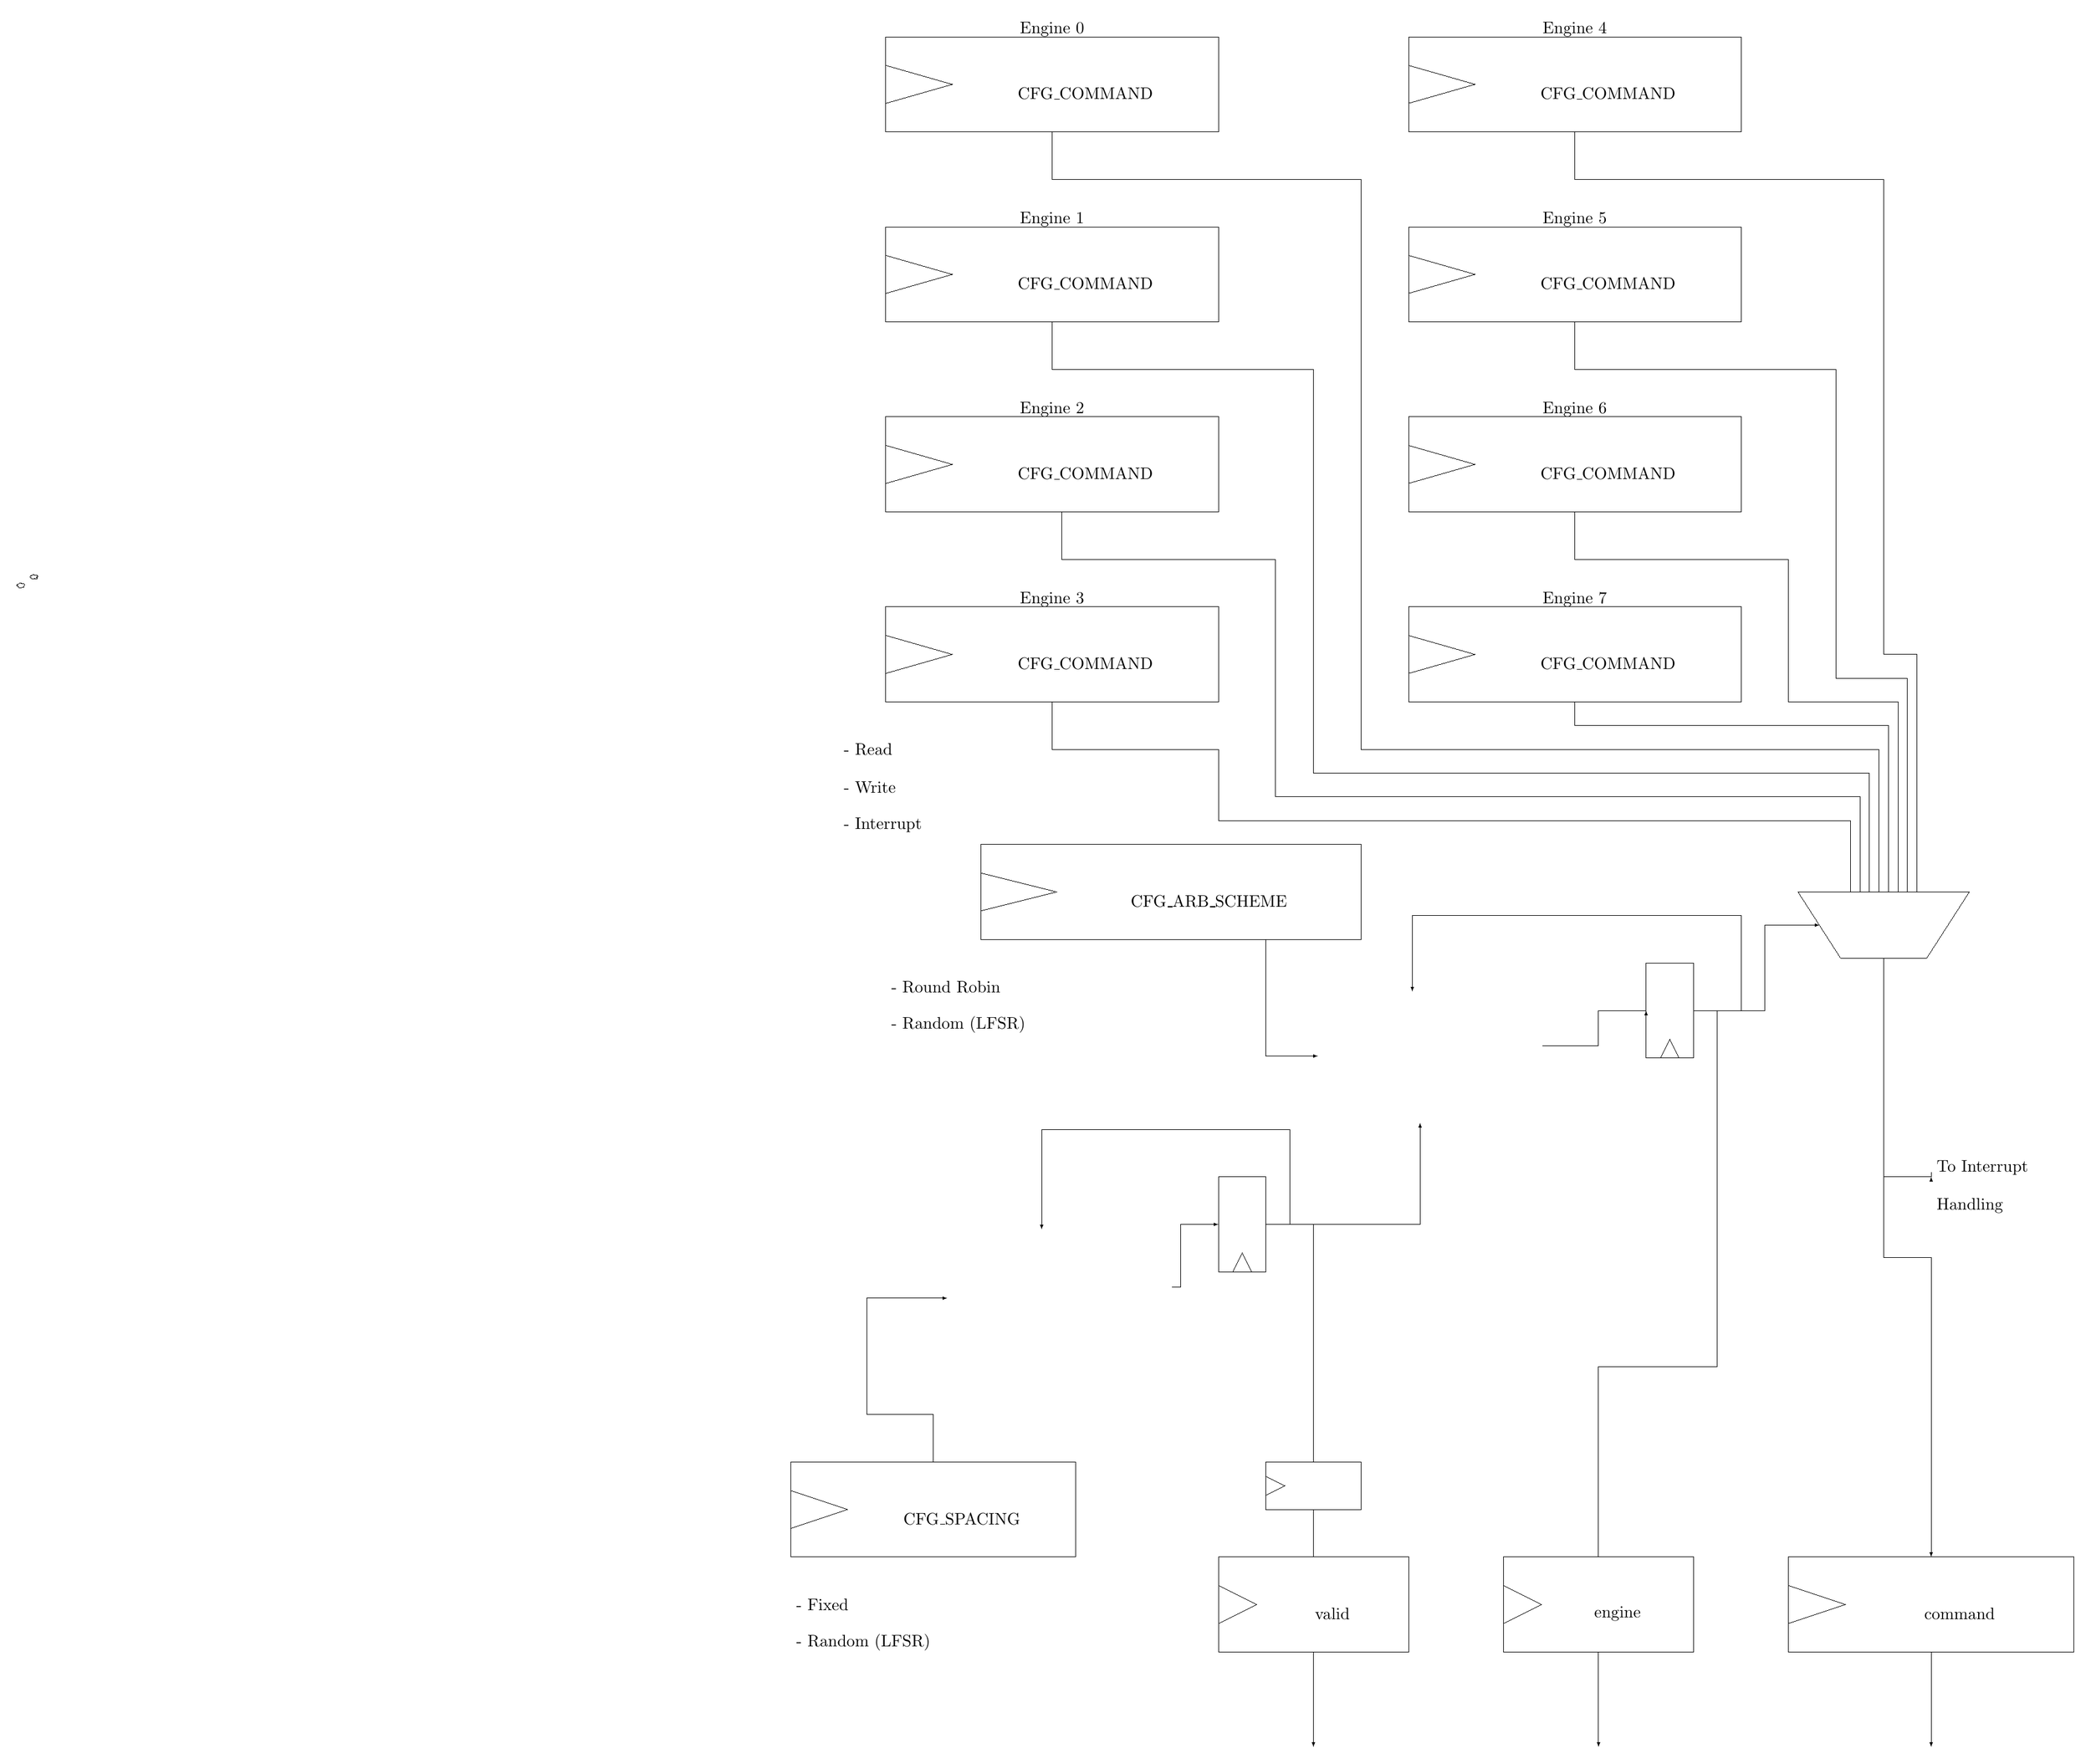
\begin{tikzpicture}
\pgftransformxscale{1.000000}
\pgftransformyscale{-1.000000}
\definecolor{dialinecolor}{rgb}{0.000000, 0.000000, 0.000000}
\pgfsetstrokecolor{dialinecolor}
\definecolor{dialinecolor}{rgb}{1.000000, 1.000000, 1.000000}
\pgfsetfillcolor{dialinecolor}
\pgfsetlinewidth{0.000000\du}
\pgfsetdash{}{0pt}
\pgfsetdash{}{0pt}
\pgfsetbuttcap
\pgfsetmiterjoin
\pgfsetlinewidth{0.000000\du}
\pgfsetbuttcap
\pgfsetmiterjoin
\pgfsetdash{}{0pt}
\definecolor{dialinecolor}{rgb}{0.000000, 0.000000, 0.000000}
\pgfsetstrokecolor{dialinecolor}
\draw (19.000000\du,-11.000000\du)--(26.000000\du,-11.000000\du)--(26.000000\du,-9.000000\du)--(19.000000\du,-9.000000\du)--cycle;
\pgfsetbuttcap
\pgfsetmiterjoin
\pgfsetdash{}{0pt}
\definecolor{dialinecolor}{rgb}{0.000000, 0.000000, 0.000000}
\pgfsetstrokecolor{dialinecolor}
\draw (19.000000\du,-10.400000\du)--(20.400000\du,-10.000000\du);
\pgfsetbuttcap
\pgfsetmiterjoin
\pgfsetdash{}{0pt}
\definecolor{dialinecolor}{rgb}{0.000000, 0.000000, 0.000000}
\pgfsetstrokecolor{dialinecolor}
\draw (20.400000\du,-10.000000\du)--(19.000000\du,-9.600000\du);
% setfont left to latex
\definecolor{dialinecolor}{rgb}{0.000000, 0.000000, 0.000000}
\pgfsetstrokecolor{dialinecolor}
\node at (23.200000\du,-9.800000\du){CFG\_COMMAND};
\pgfsetlinewidth{0.000000\du}
\pgfsetdash{}{0pt}
\pgfsetdash{}{0pt}
\pgfsetbuttcap
\pgfsetmiterjoin
\pgfsetlinewidth{0.000000\du}
\pgfsetbuttcap
\pgfsetmiterjoin
\pgfsetdash{}{0pt}
\definecolor{dialinecolor}{rgb}{0.000000, 0.000000, 0.000000}
\pgfsetstrokecolor{dialinecolor}
\draw (19.000000\du,-7.000000\du)--(26.000000\du,-7.000000\du)--(26.000000\du,-5.000000\du)--(19.000000\du,-5.000000\du)--cycle;
\pgfsetbuttcap
\pgfsetmiterjoin
\pgfsetdash{}{0pt}
\definecolor{dialinecolor}{rgb}{0.000000, 0.000000, 0.000000}
\pgfsetstrokecolor{dialinecolor}
\draw (19.000000\du,-6.400000\du)--(20.400000\du,-6.000000\du);
\pgfsetbuttcap
\pgfsetmiterjoin
\pgfsetdash{}{0pt}
\definecolor{dialinecolor}{rgb}{0.000000, 0.000000, 0.000000}
\pgfsetstrokecolor{dialinecolor}
\draw (20.400000\du,-6.000000\du)--(19.000000\du,-5.600000\du);
% setfont left to latex
\definecolor{dialinecolor}{rgb}{0.000000, 0.000000, 0.000000}
\pgfsetstrokecolor{dialinecolor}
\node at (23.200000\du,-5.800000\du){CFG\_COMMAND};
\pgfsetlinewidth{0.000000\du}
\pgfsetdash{}{0pt}
\pgfsetdash{}{0pt}
\pgfsetbuttcap
\pgfsetmiterjoin
\pgfsetlinewidth{0.000000\du}
\pgfsetbuttcap
\pgfsetmiterjoin
\pgfsetdash{}{0pt}
\definecolor{dialinecolor}{rgb}{0.000000, 0.000000, 0.000000}
\pgfsetstrokecolor{dialinecolor}
\draw (19.000000\du,-3.000000\du)--(26.000000\du,-3.000000\du)--(26.000000\du,-1.000000\du)--(19.000000\du,-1.000000\du)--cycle;
\pgfsetbuttcap
\pgfsetmiterjoin
\pgfsetdash{}{0pt}
\definecolor{dialinecolor}{rgb}{0.000000, 0.000000, 0.000000}
\pgfsetstrokecolor{dialinecolor}
\draw (19.000000\du,-2.400000\du)--(20.400000\du,-2.000000\du);
\pgfsetbuttcap
\pgfsetmiterjoin
\pgfsetdash{}{0pt}
\definecolor{dialinecolor}{rgb}{0.000000, 0.000000, 0.000000}
\pgfsetstrokecolor{dialinecolor}
\draw (20.400000\du,-2.000000\du)--(19.000000\du,-1.600000\du);
% setfont left to latex
\definecolor{dialinecolor}{rgb}{0.000000, 0.000000, 0.000000}
\pgfsetstrokecolor{dialinecolor}
\node at (23.200000\du,-1.800000\du){CFG\_COMMAND};
\pgfsetlinewidth{0.000000\du}
\pgfsetdash{}{0pt}
\pgfsetdash{}{0pt}
\pgfsetbuttcap
\pgfsetmiterjoin
\pgfsetlinewidth{0.000000\du}
\pgfsetbuttcap
\pgfsetmiterjoin
\pgfsetdash{}{0pt}
\definecolor{dialinecolor}{rgb}{0.000000, 0.000000, 0.000000}
\pgfsetstrokecolor{dialinecolor}
\draw (19.000000\du,1.000000\du)--(26.000000\du,1.000000\du)--(26.000000\du,3.000000\du)--(19.000000\du,3.000000\du)--cycle;
\pgfsetbuttcap
\pgfsetmiterjoin
\pgfsetdash{}{0pt}
\definecolor{dialinecolor}{rgb}{0.000000, 0.000000, 0.000000}
\pgfsetstrokecolor{dialinecolor}
\draw (19.000000\du,1.600000\du)--(20.400000\du,2.000000\du);
\pgfsetbuttcap
\pgfsetmiterjoin
\pgfsetdash{}{0pt}
\definecolor{dialinecolor}{rgb}{0.000000, 0.000000, 0.000000}
\pgfsetstrokecolor{dialinecolor}
\draw (20.400000\du,2.000000\du)--(19.000000\du,2.400000\du);
% setfont left to latex
\definecolor{dialinecolor}{rgb}{0.000000, 0.000000, 0.000000}
\pgfsetstrokecolor{dialinecolor}
\node at (23.200000\du,2.200000\du){CFG\_COMMAND};
\pgfsetlinewidth{0.000000\du}
\pgfsetdash{}{0pt}
\pgfsetdash{}{0pt}
\pgfsetbuttcap
\pgfsetmiterjoin
\pgfsetlinewidth{0.000000\du}
\pgfsetbuttcap
\pgfsetmiterjoin
\pgfsetdash{}{0pt}
\definecolor{dialinecolor}{rgb}{0.000000, 0.000000, 0.000000}
\pgfsetstrokecolor{dialinecolor}
\draw (30.000000\du,-11.000000\du)--(37.000000\du,-11.000000\du)--(37.000000\du,-9.000000\du)--(30.000000\du,-9.000000\du)--cycle;
\pgfsetbuttcap
\pgfsetmiterjoin
\pgfsetdash{}{0pt}
\definecolor{dialinecolor}{rgb}{0.000000, 0.000000, 0.000000}
\pgfsetstrokecolor{dialinecolor}
\draw (30.000000\du,-10.400000\du)--(31.400000\du,-10.000000\du);
\pgfsetbuttcap
\pgfsetmiterjoin
\pgfsetdash{}{0pt}
\definecolor{dialinecolor}{rgb}{0.000000, 0.000000, 0.000000}
\pgfsetstrokecolor{dialinecolor}
\draw (31.400000\du,-10.000000\du)--(30.000000\du,-9.600000\du);
% setfont left to latex
\definecolor{dialinecolor}{rgb}{0.000000, 0.000000, 0.000000}
\pgfsetstrokecolor{dialinecolor}
\node at (34.200000\du,-9.800000\du){CFG\_COMMAND};
\pgfsetlinewidth{0.000000\du}
\pgfsetdash{}{0pt}
\pgfsetdash{}{0pt}
\pgfsetbuttcap
\pgfsetmiterjoin
\pgfsetlinewidth{0.000000\du}
\pgfsetbuttcap
\pgfsetmiterjoin
\pgfsetdash{}{0pt}
\definecolor{dialinecolor}{rgb}{0.000000, 0.000000, 0.000000}
\pgfsetstrokecolor{dialinecolor}
\draw (30.000000\du,-7.000000\du)--(37.000000\du,-7.000000\du)--(37.000000\du,-5.000000\du)--(30.000000\du,-5.000000\du)--cycle;
\pgfsetbuttcap
\pgfsetmiterjoin
\pgfsetdash{}{0pt}
\definecolor{dialinecolor}{rgb}{0.000000, 0.000000, 0.000000}
\pgfsetstrokecolor{dialinecolor}
\draw (30.000000\du,-6.400000\du)--(31.400000\du,-6.000000\du);
\pgfsetbuttcap
\pgfsetmiterjoin
\pgfsetdash{}{0pt}
\definecolor{dialinecolor}{rgb}{0.000000, 0.000000, 0.000000}
\pgfsetstrokecolor{dialinecolor}
\draw (31.400000\du,-6.000000\du)--(30.000000\du,-5.600000\du);
% setfont left to latex
\definecolor{dialinecolor}{rgb}{0.000000, 0.000000, 0.000000}
\pgfsetstrokecolor{dialinecolor}
\node at (34.200000\du,-5.800000\du){CFG\_COMMAND};
\pgfsetlinewidth{0.000000\du}
\pgfsetdash{}{0pt}
\pgfsetdash{}{0pt}
\pgfsetbuttcap
\pgfsetmiterjoin
\pgfsetlinewidth{0.000000\du}
\pgfsetbuttcap
\pgfsetmiterjoin
\pgfsetdash{}{0pt}
\definecolor{dialinecolor}{rgb}{0.000000, 0.000000, 0.000000}
\pgfsetstrokecolor{dialinecolor}
\draw (30.000000\du,-3.000000\du)--(37.000000\du,-3.000000\du)--(37.000000\du,-1.000000\du)--(30.000000\du,-1.000000\du)--cycle;
\pgfsetbuttcap
\pgfsetmiterjoin
\pgfsetdash{}{0pt}
\definecolor{dialinecolor}{rgb}{0.000000, 0.000000, 0.000000}
\pgfsetstrokecolor{dialinecolor}
\draw (30.000000\du,-2.400000\du)--(31.400000\du,-2.000000\du);
\pgfsetbuttcap
\pgfsetmiterjoin
\pgfsetdash{}{0pt}
\definecolor{dialinecolor}{rgb}{0.000000, 0.000000, 0.000000}
\pgfsetstrokecolor{dialinecolor}
\draw (31.400000\du,-2.000000\du)--(30.000000\du,-1.600000\du);
% setfont left to latex
\definecolor{dialinecolor}{rgb}{0.000000, 0.000000, 0.000000}
\pgfsetstrokecolor{dialinecolor}
\node at (34.200000\du,-1.800000\du){CFG\_COMMAND};
\pgfsetlinewidth{0.000000\du}
\pgfsetdash{}{0pt}
\pgfsetdash{}{0pt}
\pgfsetbuttcap
\pgfsetmiterjoin
\pgfsetlinewidth{0.000000\du}
\pgfsetbuttcap
\pgfsetmiterjoin
\pgfsetdash{}{0pt}
\definecolor{dialinecolor}{rgb}{0.000000, 0.000000, 0.000000}
\pgfsetstrokecolor{dialinecolor}
\draw (30.000000\du,1.000000\du)--(37.000000\du,1.000000\du)--(37.000000\du,3.000000\du)--(30.000000\du,3.000000\du)--cycle;
\pgfsetbuttcap
\pgfsetmiterjoin
\pgfsetdash{}{0pt}
\definecolor{dialinecolor}{rgb}{0.000000, 0.000000, 0.000000}
\pgfsetstrokecolor{dialinecolor}
\draw (30.000000\du,1.600000\du)--(31.400000\du,2.000000\du);
\pgfsetbuttcap
\pgfsetmiterjoin
\pgfsetdash{}{0pt}
\definecolor{dialinecolor}{rgb}{0.000000, 0.000000, 0.000000}
\pgfsetstrokecolor{dialinecolor}
\draw (31.400000\du,2.000000\du)--(30.000000\du,2.400000\du);
% setfont left to latex
\definecolor{dialinecolor}{rgb}{0.000000, 0.000000, 0.000000}
\pgfsetstrokecolor{dialinecolor}
\node at (34.200000\du,2.200000\du){CFG\_COMMAND};
\pgfsetlinewidth{0.000000\du}
\pgfsetdash{}{0pt}
\pgfsetdash{}{0pt}
\pgfsetbuttcap
\pgfsetmiterjoin
\pgfsetlinewidth{0.000000\du}
\pgfsetbuttcap
\pgfsetmiterjoin
\pgfsetdash{}{0pt}
\definecolor{dialinecolor}{rgb}{0.000000, 0.000000, 0.000000}
\pgfsetstrokecolor{dialinecolor}
\draw (38.200000\du,7.000000\du)--(41.800000\du,7.000000\du)--(40.900000\du,8.400000\du)--(39.100000\du,8.400000\du)--cycle;
% setfont left to latex
\definecolor{dialinecolor}{rgb}{0.000000, 0.000000, 0.000000}
\pgfsetstrokecolor{dialinecolor}
\node at (40.000000\du,7.900000\du){};
\pgfsetlinewidth{0.000000\du}
\pgfsetdash{}{0pt}
\pgfsetdash{}{0pt}
\pgfsetbuttcap
{
\definecolor{dialinecolor}{rgb}{0.000000, 0.000000, 0.000000}
\pgfsetfillcolor{dialinecolor}
% was here!!!
\definecolor{dialinecolor}{rgb}{0.000000, 0.000000, 0.000000}
\pgfsetstrokecolor{dialinecolor}
\draw (39.100000\du,7.000000\du)--(40.900000\du,7.000000\du);
}
\pgfsetlinewidth{0.000000\du}
\pgfsetdash{}{0pt}
\pgfsetdash{}{0pt}
\pgfsetmiterjoin
\pgfsetbuttcap
{
\definecolor{dialinecolor}{rgb}{0.000000, 0.000000, 0.000000}
\pgfsetfillcolor{dialinecolor}
% was here!!!
{\pgfsetcornersarced{\pgfpoint{0.000000\du}{0.000000\du}}\definecolor{dialinecolor}{rgb}{0.000000, 0.000000, 0.000000}
\pgfsetstrokecolor{dialinecolor}
\draw (22.500000\du,-9.000000\du)--(22.500000\du,-8.000000\du)--(29.000000\du,-8.000000\du)--(29.000000\du,4.000000\du)--(39.900000\du,4.000000\du)--(39.900000\du,7.000000\du)--(39.900000\du,7.000000\du);
}}
\pgfsetlinewidth{0.000000\du}
\pgfsetdash{}{0pt}
\pgfsetdash{}{0pt}
\pgfsetmiterjoin
\pgfsetbuttcap
{
\definecolor{dialinecolor}{rgb}{0.000000, 0.000000, 0.000000}
\pgfsetfillcolor{dialinecolor}
% was here!!!
{\pgfsetcornersarced{\pgfpoint{0.000000\du}{0.000000\du}}\definecolor{dialinecolor}{rgb}{0.000000, 0.000000, 0.000000}
\pgfsetstrokecolor{dialinecolor}
\draw (22.500000\du,-5.000000\du)--(22.500000\du,-4.000000\du)--(28.000000\du,-4.000000\du)--(28.000000\du,4.500000\du)--(39.700000\du,4.500000\du)--(39.700000\du,7.000000\du)--(39.700000\du,7.000000\du);
}}
\pgfsetlinewidth{0.000000\du}
\pgfsetdash{}{0pt}
\pgfsetdash{}{0pt}
\pgfsetmiterjoin
\pgfsetbuttcap
{
\definecolor{dialinecolor}{rgb}{0.000000, 0.000000, 0.000000}
\pgfsetfillcolor{dialinecolor}
% was here!!!
{\pgfsetcornersarced{\pgfpoint{0.000000\du}{0.000000\du}}\definecolor{dialinecolor}{rgb}{0.000000, 0.000000, 0.000000}
\pgfsetstrokecolor{dialinecolor}
\draw (22.700000\du,-1.000000\du)--(22.700000\du,0.000000\du)--(27.200000\du,0.000000\du)--(27.200000\du,5.000000\du)--(39.500000\du,5.000000\du)--(39.500000\du,7.000000\du)--(39.500000\du,7.000000\du);
}}
\pgfsetlinewidth{0.000000\du}
\pgfsetdash{}{0pt}
\pgfsetdash{}{0pt}
\pgfsetmiterjoin
\pgfsetbuttcap
{
\definecolor{dialinecolor}{rgb}{0.000000, 0.000000, 0.000000}
\pgfsetfillcolor{dialinecolor}
% was here!!!
{\pgfsetcornersarced{\pgfpoint{0.000000\du}{0.000000\du}}\definecolor{dialinecolor}{rgb}{0.000000, 0.000000, 0.000000}
\pgfsetstrokecolor{dialinecolor}
\draw (22.500000\du,3.000000\du)--(22.500000\du,4.000000\du)--(26.000000\du,4.000000\du)--(26.000000\du,5.500000\du)--(39.300000\du,5.500000\du)--(39.300000\du,7.000000\du)--(39.300000\du,7.000000\du);
}}
\pgfsetlinewidth{0.000000\du}
\pgfsetdash{}{0pt}
\pgfsetdash{}{0pt}
\pgfsetmiterjoin
\pgfsetbuttcap
{
\definecolor{dialinecolor}{rgb}{0.000000, 0.000000, 0.000000}
\pgfsetfillcolor{dialinecolor}
% was here!!!
{\pgfsetcornersarced{\pgfpoint{0.000000\du}{0.000000\du}}\definecolor{dialinecolor}{rgb}{0.000000, 0.000000, 0.000000}
\pgfsetstrokecolor{dialinecolor}
\draw (33.500000\du,3.000000\du)--(33.500000\du,3.500000\du)--(40.100000\du,3.500000\du)--(40.100000\du,7.000000\du);
}}
\pgfsetlinewidth{0.000000\du}
\pgfsetdash{}{0pt}
\pgfsetdash{}{0pt}
\pgfsetmiterjoin
\pgfsetbuttcap
{
\definecolor{dialinecolor}{rgb}{0.000000, 0.000000, 0.000000}
\pgfsetfillcolor{dialinecolor}
% was here!!!
{\pgfsetcornersarced{\pgfpoint{0.000000\du}{0.000000\du}}\definecolor{dialinecolor}{rgb}{0.000000, 0.000000, 0.000000}
\pgfsetstrokecolor{dialinecolor}
\draw (33.500000\du,-1.000000\du)--(33.500000\du,0.000000\du)--(38.000000\du,0.000000\du)--(38.000000\du,3.000000\du)--(40.300000\du,3.000000\du)--(40.300000\du,7.000000\du)--(40.300000\du,7.000000\du);
}}
\pgfsetlinewidth{0.000000\du}
\pgfsetdash{}{0pt}
\pgfsetdash{}{0pt}
\pgfsetmiterjoin
\pgfsetbuttcap
{
\definecolor{dialinecolor}{rgb}{0.000000, 0.000000, 0.000000}
\pgfsetfillcolor{dialinecolor}
% was here!!!
{\pgfsetcornersarced{\pgfpoint{0.000000\du}{0.000000\du}}\definecolor{dialinecolor}{rgb}{0.000000, 0.000000, 0.000000}
\pgfsetstrokecolor{dialinecolor}
\draw (33.500000\du,-5.000000\du)--(33.500000\du,-4.000000\du)--(39.000000\du,-4.000000\du)--(39.000000\du,2.500000\du)--(40.500000\du,2.500000\du)--(40.500000\du,7.000000\du);
}}
\pgfsetlinewidth{0.000000\du}
\pgfsetdash{}{0pt}
\pgfsetdash{}{0pt}
\pgfsetmiterjoin
\pgfsetbuttcap
{
\definecolor{dialinecolor}{rgb}{0.000000, 0.000000, 0.000000}
\pgfsetfillcolor{dialinecolor}
% was here!!!
{\pgfsetcornersarced{\pgfpoint{0.000000\du}{0.000000\du}}\definecolor{dialinecolor}{rgb}{0.000000, 0.000000, 0.000000}
\pgfsetstrokecolor{dialinecolor}
\draw (33.500000\du,-9.000000\du)--(33.500000\du,-8.000000\du)--(40.000000\du,-8.000000\du)--(40.000000\du,2.000000\du)--(40.700000\du,2.000000\du)--(40.700000\du,7.000000\du);
}}
% setfont left to latex
\definecolor{dialinecolor}{rgb}{0.000000, 0.000000, 0.000000}
\pgfsetstrokecolor{dialinecolor}
\node at (22.500000\du,-11.152500\du){Engine 0};
% setfont left to latex
\definecolor{dialinecolor}{rgb}{0.000000, 0.000000, 0.000000}
\pgfsetstrokecolor{dialinecolor}
\node at (22.500000\du,-7.152500\du){Engine 1};
% setfont left to latex
\definecolor{dialinecolor}{rgb}{0.000000, 0.000000, 0.000000}
\pgfsetstrokecolor{dialinecolor}
\node at (22.500000\du,-3.152500\du){Engine 2};
% setfont left to latex
\definecolor{dialinecolor}{rgb}{0.000000, 0.000000, 0.000000}
\pgfsetstrokecolor{dialinecolor}
\node at (22.500000\du,0.847500\du){Engine 3};
% setfont left to latex
\definecolor{dialinecolor}{rgb}{0.000000, 0.000000, 0.000000}
\pgfsetstrokecolor{dialinecolor}
\node at (33.500000\du,-11.152500\du){Engine 4};
% setfont left to latex
\definecolor{dialinecolor}{rgb}{0.000000, 0.000000, 0.000000}
\pgfsetstrokecolor{dialinecolor}
\node at (33.500000\du,-7.152500\du){Engine 5};
% setfont left to latex
\definecolor{dialinecolor}{rgb}{0.000000, 0.000000, 0.000000}
\pgfsetstrokecolor{dialinecolor}
\node at (33.500000\du,-3.152500\du){Engine 6};
% setfont left to latex
\definecolor{dialinecolor}{rgb}{0.000000, 0.000000, 0.000000}
\pgfsetstrokecolor{dialinecolor}
\node at (33.500000\du,0.847500\du){Engine 7};
\pgfsetlinewidth{0.000000\du}
\pgfsetdash{}{0pt}
\pgfsetdash{}{0pt}
\pgfsetbuttcap
\pgfsetmiterjoin
\pgfsetlinewidth{0.000000\du}
\pgfsetbuttcap
\pgfsetmiterjoin
\pgfsetdash{}{0pt}
\definecolor{dialinecolor}{rgb}{0.000000, 0.000000, 0.000000}
\pgfsetstrokecolor{dialinecolor}
\draw (38.000000\du,21.000000\du)--(44.000000\du,21.000000\du)--(44.000000\du,23.000000\du)--(38.000000\du,23.000000\du)--cycle;
\pgfsetbuttcap
\pgfsetmiterjoin
\pgfsetdash{}{0pt}
\definecolor{dialinecolor}{rgb}{0.000000, 0.000000, 0.000000}
\pgfsetstrokecolor{dialinecolor}
\draw (38.000000\du,21.600000\du)--(39.200000\du,22.000000\du);
\pgfsetbuttcap
\pgfsetmiterjoin
\pgfsetdash{}{0pt}
\definecolor{dialinecolor}{rgb}{0.000000, 0.000000, 0.000000}
\pgfsetstrokecolor{dialinecolor}
\draw (39.200000\du,22.000000\du)--(38.000000\du,22.400000\du);
% setfont left to latex
\definecolor{dialinecolor}{rgb}{0.000000, 0.000000, 0.000000}
\pgfsetstrokecolor{dialinecolor}
\node at (41.600000\du,22.200000\du){command};
\pgfsetlinewidth{0.000000\du}
\pgfsetdash{}{0pt}
\pgfsetdash{}{0pt}
\pgfsetbuttcap
{
\definecolor{dialinecolor}{rgb}{0.000000, 0.000000, 0.000000}
\pgfsetfillcolor{dialinecolor}
% was here!!!
\pgfsetarrowsend{latex}
\definecolor{dialinecolor}{rgb}{0.000000, 0.000000, 0.000000}
\pgfsetstrokecolor{dialinecolor}
\draw (41.000000\du,23.000000\du)--(41.000000\du,25.000000\du);
}
\pgfsetlinewidth{0.000000\du}
\pgfsetdash{}{0pt}
\pgfsetdash{}{0pt}
\pgfsetbuttcap
\pgfsetmiterjoin
\pgfsetlinewidth{0.000000\du}
\pgfsetbuttcap
\pgfsetmiterjoin
\pgfsetdash{}{0pt}
\definecolor{dialinecolor}{rgb}{0.000000, 0.000000, 0.000000}
\pgfsetstrokecolor{dialinecolor}
\draw (21.000000\du,6.000000\du)--(29.000000\du,6.000000\du)--(29.000000\du,8.000000\du)--(21.000000\du,8.000000\du)--cycle;
\pgfsetbuttcap
\pgfsetmiterjoin
\pgfsetdash{}{0pt}
\definecolor{dialinecolor}{rgb}{0.000000, 0.000000, 0.000000}
\pgfsetstrokecolor{dialinecolor}
\draw (21.000000\du,6.600000\du)--(22.600000\du,7.000000\du);
\pgfsetbuttcap
\pgfsetmiterjoin
\pgfsetdash{}{0pt}
\definecolor{dialinecolor}{rgb}{0.000000, 0.000000, 0.000000}
\pgfsetstrokecolor{dialinecolor}
\draw (22.600000\du,7.000000\du)--(21.000000\du,7.400000\du);
% setfont left to latex
\definecolor{dialinecolor}{rgb}{0.000000, 0.000000, 0.000000}
\pgfsetstrokecolor{dialinecolor}
\node at (25.800000\du,7.200000\du){CFG\_ARB\_SCHEME};
\pgfsetlinewidth{0.000000\du}
\pgfsetdash{}{0pt}
\pgfsetdash{}{0pt}
\pgfsetbuttcap
\pgfsetmiterjoin
\pgfsetlinewidth{0.000000\du}
\pgfsetbuttcap
\pgfsetmiterjoin
\pgfsetdash{}{0pt}
\definecolor{dialinecolor}{rgb}{0.000000, 0.000000, 0.000000}
\pgfsetstrokecolor{dialinecolor}
\draw (35.000000\du,8.500000\du)--(36.000000\du,8.500000\du)--(36.000000\du,10.500000\du)--(35.000000\du,10.500000\du)--cycle;
\pgfsetbuttcap
\pgfsetmiterjoin
\pgfsetdash{}{0pt}
\definecolor{dialinecolor}{rgb}{0.000000, 0.000000, 0.000000}
\pgfsetstrokecolor{dialinecolor}
\draw (35.300000\du,10.500000\du)--(35.500000\du,10.100000\du);
\pgfsetbuttcap
\pgfsetmiterjoin
\pgfsetdash{}{0pt}
\definecolor{dialinecolor}{rgb}{0.000000, 0.000000, 0.000000}
\pgfsetstrokecolor{dialinecolor}
\draw (35.500000\du,10.100000\du)--(35.700000\du,10.500000\du);
% setfont left to latex
\definecolor{dialinecolor}{rgb}{0.000000, 0.000000, 0.000000}
\pgfsetstrokecolor{dialinecolor}
\node at (35.500000\du,9.500000\du){};
\pgfsetlinewidth{0.000000\du}
\pgfsetdash{}{0pt}
\pgfsetdash{}{0pt}
\pgfsetbuttcap
\pgfsetmiterjoin
\pgfsetlinewidth{0.000000\du}
\pgfsetbuttcap
\pgfsetmiterjoin
\pgfsetdash{}{0pt}
\definecolor{dialinecolor}{rgb}{0.000000, 0.000000, 0.000000}
\pgfsetstrokecolor{dialinecolor}
\draw (32.000000\du,21.000000\du)--(36.000000\du,21.000000\du)--(36.000000\du,23.000000\du)--(32.000000\du,23.000000\du)--cycle;
\pgfsetbuttcap
\pgfsetmiterjoin
\pgfsetdash{}{0pt}
\definecolor{dialinecolor}{rgb}{0.000000, 0.000000, 0.000000}
\pgfsetstrokecolor{dialinecolor}
\draw (32.000000\du,21.600000\du)--(32.800000\du,22.000000\du);
\pgfsetbuttcap
\pgfsetmiterjoin
\pgfsetdash{}{0pt}
\definecolor{dialinecolor}{rgb}{0.000000, 0.000000, 0.000000}
\pgfsetstrokecolor{dialinecolor}
\draw (32.800000\du,22.000000\du)--(32.000000\du,22.400000\du);
% setfont left to latex
\definecolor{dialinecolor}{rgb}{0.000000, 0.000000, 0.000000}
\pgfsetstrokecolor{dialinecolor}
\node at (34.400000\du,22.200000\du){engine};
\pgfsetlinewidth{0.000000\du}
\pgfsetdash{}{0pt}
\pgfsetdash{}{0pt}
\pgfsetmiterjoin
\pgfsetbuttcap
{
\definecolor{dialinecolor}{rgb}{0.000000, 0.000000, 0.000000}
\pgfsetfillcolor{dialinecolor}
% was here!!!
{\pgfsetcornersarced{\pgfpoint{0.000000\du}{0.000000\du}}\definecolor{dialinecolor}{rgb}{0.000000, 0.000000, 0.000000}
\pgfsetstrokecolor{dialinecolor}
\draw (36.000000\du,9.500000\du)--(36.500000\du,9.500000\du)--(36.500000\du,17.000000\du)--(34.000000\du,17.000000\du)--(34.000000\du,21.000000\du);
}}
\pgfsetlinewidth{0.000000\du}
\pgfsetdash{}{0pt}
\pgfsetdash{}{0pt}
\pgfsetmiterjoin
\pgfsetbuttcap
{
\definecolor{dialinecolor}{rgb}{0.000000, 0.000000, 0.000000}
\pgfsetfillcolor{dialinecolor}
% was here!!!
\pgfsetarrowsend{latex}
{\pgfsetcornersarced{\pgfpoint{0.000000\du}{0.000000\du}}\definecolor{dialinecolor}{rgb}{0.000000, 0.000000, 0.000000}
\pgfsetstrokecolor{dialinecolor}
\draw (36.000000\du,9.500000\du)--(37.500000\du,9.500000\du)--(37.500000\du,7.700000\du)--(38.650000\du,7.700000\du);
}}
\pgfsetlinewidth{0.000000\du}
\pgfsetdash{}{0pt}
\pgfsetdash{}{0pt}
\pgfsetbuttcap
{
\definecolor{dialinecolor}{rgb}{0.000000, 0.000000, 0.000000}
\pgfsetfillcolor{dialinecolor}
% was here!!!
\pgfsetarrowsend{latex}
\definecolor{dialinecolor}{rgb}{0.000000, 0.000000, 0.000000}
\pgfsetstrokecolor{dialinecolor}
\draw (34.000000\du,23.000000\du)--(34.000000\du,25.000000\du);
}
\pgfsetlinewidth{0.000000\du}
\pgfsetdash{}{0pt}
\pgfsetdash{}{0pt}
\pgfsetbuttcap
\pgfsetmiterjoin
\pgfsetlinewidth{0.000000\du}
\pgfsetbuttcap
\pgfsetmiterjoin
\pgfsetdash{}{0pt}
\definecolor{dialinecolor}{rgb}{1.000000, 1.000000, 1.000000}
\pgfsetfillcolor{dialinecolor}
\pgfpathmoveto{\pgfpoint{29.138499\du}{9.871624\du}}
\pgfpathcurveto{\pgfpoint{28.751174\du}{9.861488\du}}{\pgfpoint{28.000000\du}{10.074326\du}}{\pgfpoint{28.105634\du}{10.530408\du}}
\pgfpathcurveto{\pgfpoint{28.211267\du}{10.986490\du}}{\pgfpoint{28.715963\du}{11.087837\du}}{\pgfpoint{28.927231\du}{10.956084\du}}
\pgfpathcurveto{\pgfpoint{29.138499\du}{10.824327\du}}{\pgfpoint{28.598592\du}{11.594594\du}}{\pgfpoint{29.631458\du}{11.797297\du}}
\pgfpathcurveto{\pgfpoint{30.664314\du}{12.000000\du}}{\pgfpoint{31.192484\du}{11.675675\du}}{\pgfpoint{31.039902\du}{11.442567\du}}
\pgfpathcurveto{\pgfpoint{30.887319\du}{11.209459\du}}{\pgfpoint{31.943660\du}{11.989865\du}}{\pgfpoint{32.436619\du}{11.543918\du}}
\pgfpathcurveto{\pgfpoint{32.929577\du}{11.097972\du}}{\pgfpoint{31.931923\du}{10.672300\du}}{\pgfpoint{32.143191\du}{10.733111\du}}
\pgfpathcurveto{\pgfpoint{32.354459\du}{10.793922\du}}{\pgfpoint{33.000000\du}{10.712841\du}}{\pgfpoint{32.788732\du}{9.952705\du}}
\pgfpathcurveto{\pgfpoint{32.577464\du}{9.192569\du}}{\pgfpoint{30.676051\du}{9.780407\du}}{\pgfpoint{30.887319\du}{9.668921\du}}
\pgfpathcurveto{\pgfpoint{31.098588\du}{9.557434\du}}{\pgfpoint{30.570417\du}{9.000000\du}}{\pgfpoint{29.913148\du}{9.111487\du}}
\pgfpathcurveto{\pgfpoint{29.255870\du}{9.222974\du}}{\pgfpoint{29.209250\du}{9.425282\du}}{\pgfpoint{29.138828\du}{9.871228\du}}
\pgfpathlineto{\pgfpoint{29.138499\du}{9.871624\du}}
\pgfusepath{fill}
\definecolor{dialinecolor}{rgb}{0.000000, 0.000000, 0.000000}
\pgfsetstrokecolor{dialinecolor}
\pgfpathmoveto{\pgfpoint{29.138499\du}{9.871624\du}}
\pgfpathcurveto{\pgfpoint{28.751174\du}{9.861488\du}}{\pgfpoint{28.000000\du}{10.074326\du}}{\pgfpoint{28.105634\du}{10.530408\du}}
\pgfpathcurveto{\pgfpoint{28.211267\du}{10.986490\du}}{\pgfpoint{28.715963\du}{11.087837\du}}{\pgfpoint{28.927231\du}{10.956084\du}}
\pgfpathcurveto{\pgfpoint{29.138499\du}{10.824327\du}}{\pgfpoint{28.598592\du}{11.594594\du}}{\pgfpoint{29.631458\du}{11.797297\du}}
\pgfpathcurveto{\pgfpoint{30.664314\du}{12.000000\du}}{\pgfpoint{31.192484\du}{11.675675\du}}{\pgfpoint{31.039902\du}{11.442567\du}}
\pgfpathcurveto{\pgfpoint{30.887319\du}{11.209459\du}}{\pgfpoint{31.943660\du}{11.989865\du}}{\pgfpoint{32.436619\du}{11.543918\du}}
\pgfpathcurveto{\pgfpoint{32.929577\du}{11.097972\du}}{\pgfpoint{31.931923\du}{10.672300\du}}{\pgfpoint{32.143191\du}{10.733111\du}}
\pgfpathcurveto{\pgfpoint{32.354459\du}{10.793922\du}}{\pgfpoint{33.000000\du}{10.712841\du}}{\pgfpoint{32.788732\du}{9.952705\du}}
\pgfpathcurveto{\pgfpoint{32.577464\du}{9.192569\du}}{\pgfpoint{30.676051\du}{9.780407\du}}{\pgfpoint{30.887319\du}{9.668921\du}}
\pgfpathcurveto{\pgfpoint{31.098588\du}{9.557434\du}}{\pgfpoint{30.570417\du}{9.000000\du}}{\pgfpoint{29.913148\du}{9.111487\du}}
\pgfpathcurveto{\pgfpoint{29.255870\du}{9.222974\du}}{\pgfpoint{29.209250\du}{9.425282\du}}{\pgfpoint{29.138828\du}{9.871228\du}}
\pgfpathlineto{\pgfpoint{29.138499\du}{9.871624\du}}
\pgfusepath{stroke}
% setfont left to latex
\definecolor{dialinecolor}{rgb}{0.000000, 0.000000, 0.000000}
\pgfsetstrokecolor{dialinecolor}
\node at (30.634033\du,10.752884\du){};
\pgfsetlinewidth{0.000000\du}
\pgfsetdash{}{0pt}
\pgfsetdash{}{0pt}
\pgfsetmiterjoin
\pgfsetbuttcap
{
\definecolor{dialinecolor}{rgb}{0.000000, 0.000000, 0.000000}
\pgfsetfillcolor{dialinecolor}
% was here!!!
\pgfsetarrowsend{latex}
{\pgfsetcornersarced{\pgfpoint{0.000000\du}{0.000000\du}}\definecolor{dialinecolor}{rgb}{0.000000, 0.000000, 0.000000}
\pgfsetstrokecolor{dialinecolor}
\draw (32.828500\du,10.237700\du)--(34.000000\du,10.237700\du)--(34.000000\du,9.500000\du)--(35.000000\du,9.500000\du)--(35.000000\du,9.500000\du);
}}
\pgfsetlinewidth{0.000000\du}
\pgfsetdash{}{0pt}
\pgfsetdash{}{0pt}
\pgfsetmiterjoin
\pgfsetbuttcap
{
\definecolor{dialinecolor}{rgb}{0.000000, 0.000000, 0.000000}
\pgfsetfillcolor{dialinecolor}
% was here!!!
\pgfsetarrowsend{latex}
{\pgfsetcornersarced{\pgfpoint{0.000000\du}{0.000000\du}}\definecolor{dialinecolor}{rgb}{0.000000, 0.000000, 0.000000}
\pgfsetstrokecolor{dialinecolor}
\draw (36.000000\du,9.500000\du)--(37.000000\du,9.500000\du)--(37.000000\du,7.500000\du)--(30.080200\du,7.500000\du)--(30.080200\du,9.097800\du);
}}
\pgfsetlinewidth{0.000000\du}
\pgfsetdash{}{0pt}
\pgfsetdash{}{0pt}
\pgfsetmiterjoin
\pgfsetbuttcap
{
\definecolor{dialinecolor}{rgb}{0.000000, 0.000000, 0.000000}
\pgfsetfillcolor{dialinecolor}
% was here!!!
\pgfsetarrowsend{latex}
{\pgfsetcornersarced{\pgfpoint{0.000000\du}{0.000000\du}}\definecolor{dialinecolor}{rgb}{0.000000, 0.000000, 0.000000}
\pgfsetstrokecolor{dialinecolor}
\draw (25.000000\du,8.000000\du)--(27.000000\du,8.000000\du)--(27.000000\du,10.455600\du)--(28.093300\du,10.455600\du);
}}
\pgfsetlinewidth{0.000000\du}
\pgfsetdash{}{0pt}
\pgfsetdash{}{0pt}
\pgfsetbuttcap
\pgfsetmiterjoin
\pgfsetlinewidth{0.000000\du}
\pgfsetbuttcap
\pgfsetmiterjoin
\pgfsetdash{}{0pt}
\definecolor{dialinecolor}{rgb}{0.000000, 0.000000, 0.000000}
\pgfsetstrokecolor{dialinecolor}
\draw (17.000000\du,19.000000\du)--(23.000000\du,19.000000\du)--(23.000000\du,21.000000\du)--(17.000000\du,21.000000\du)--cycle;
\pgfsetbuttcap
\pgfsetmiterjoin
\pgfsetdash{}{0pt}
\definecolor{dialinecolor}{rgb}{0.000000, 0.000000, 0.000000}
\pgfsetstrokecolor{dialinecolor}
\draw (17.000000\du,19.600000\du)--(18.200000\du,20.000000\du);
\pgfsetbuttcap
\pgfsetmiterjoin
\pgfsetdash{}{0pt}
\definecolor{dialinecolor}{rgb}{0.000000, 0.000000, 0.000000}
\pgfsetstrokecolor{dialinecolor}
\draw (18.200000\du,20.000000\du)--(17.000000\du,20.400000\du);
% setfont left to latex
\definecolor{dialinecolor}{rgb}{0.000000, 0.000000, 0.000000}
\pgfsetstrokecolor{dialinecolor}
\node at (20.600000\du,20.200000\du){CFG\_SPACING};
\pgfsetlinewidth{0.000000\du}
\pgfsetdash{}{0pt}
\pgfsetdash{}{0pt}
\pgfsetbuttcap
\pgfsetmiterjoin
\pgfsetlinewidth{0.000000\du}
\pgfsetbuttcap
\pgfsetmiterjoin
\pgfsetdash{}{0pt}
\definecolor{dialinecolor}{rgb}{0.000000, 0.000000, 0.000000}
\pgfsetstrokecolor{dialinecolor}
\draw (26.000000\du,21.000000\du)--(30.000000\du,21.000000\du)--(30.000000\du,23.000000\du)--(26.000000\du,23.000000\du)--cycle;
\pgfsetbuttcap
\pgfsetmiterjoin
\pgfsetdash{}{0pt}
\definecolor{dialinecolor}{rgb}{0.000000, 0.000000, 0.000000}
\pgfsetstrokecolor{dialinecolor}
\draw (26.000000\du,21.600000\du)--(26.800000\du,22.000000\du);
\pgfsetbuttcap
\pgfsetmiterjoin
\pgfsetdash{}{0pt}
\definecolor{dialinecolor}{rgb}{0.000000, 0.000000, 0.000000}
\pgfsetstrokecolor{dialinecolor}
\draw (26.800000\du,22.000000\du)--(26.000000\du,22.400000\du);
% setfont left to latex
\definecolor{dialinecolor}{rgb}{0.000000, 0.000000, 0.000000}
\pgfsetstrokecolor{dialinecolor}
\node at (28.400000\du,22.200000\du){valid};
\pgfsetlinewidth{0.000000\du}
\pgfsetdash{}{0pt}
\pgfsetdash{}{0pt}
\pgfsetmiterjoin
\pgfsetbuttcap
{
\definecolor{dialinecolor}{rgb}{0.000000, 0.000000, 0.000000}
\pgfsetfillcolor{dialinecolor}
% was here!!!
{\pgfsetcornersarced{\pgfpoint{0.000000\du}{0.000000\du}}\definecolor{dialinecolor}{rgb}{0.000000, 0.000000, 0.000000}
\pgfsetstrokecolor{dialinecolor}
\draw (27.000000\du,14.000000\du)--(28.000000\du,14.000000\du)--(28.000000\du,19.000000\du);
}}
\pgfsetlinewidth{0.000000\du}
\pgfsetdash{}{0pt}
\pgfsetdash{}{0pt}
\pgfsetmiterjoin
\pgfsetbuttcap
{
\definecolor{dialinecolor}{rgb}{0.000000, 0.000000, 0.000000}
\pgfsetfillcolor{dialinecolor}
% was here!!!
\pgfsetarrowsend{latex}
{\pgfsetcornersarced{\pgfpoint{0.000000\du}{0.000000\du}}\definecolor{dialinecolor}{rgb}{0.000000, 0.000000, 0.000000}
\pgfsetstrokecolor{dialinecolor}
\draw (20.000000\du,19.000000\du)--(20.000000\du,18.000000\du)--(18.600000\du,18.000000\du)--(18.600000\du,15.552700\du)--(20.293300\du,15.552700\du);
}}
\pgfsetlinewidth{0.000000\du}
\pgfsetdash{}{0pt}
\pgfsetdash{}{0pt}
\pgfsetbuttcap
{
\definecolor{dialinecolor}{rgb}{0.000000, 0.000000, 0.000000}
\pgfsetfillcolor{dialinecolor}
% was here!!!
\pgfsetarrowsend{latex}
\definecolor{dialinecolor}{rgb}{0.000000, 0.000000, 0.000000}
\pgfsetstrokecolor{dialinecolor}
\draw (28.000000\du,23.000000\du)--(28.000000\du,25.000000\du);
}
\pgfsetlinewidth{0.000000\du}
\pgfsetdash{}{0pt}
\pgfsetdash{}{0pt}
\pgfsetmiterjoin
\pgfsetbuttcap
{
\definecolor{dialinecolor}{rgb}{0.000000, 0.000000, 0.000000}
\pgfsetfillcolor{dialinecolor}
% was here!!!
\pgfsetarrowsend{latex}
{\pgfsetcornersarced{\pgfpoint{0.000000\du}{0.000000\du}}\definecolor{dialinecolor}{rgb}{0.000000, 0.000000, 0.000000}
\pgfsetstrokecolor{dialinecolor}
\draw (27.000000\du,14.000000\du)--(30.243800\du,14.000000\du)--(30.243800\du,11.862500\du);
}}
\pgfsetlinewidth{0.000000\du}
\pgfsetdash{}{0pt}
\pgfsetdash{}{0pt}
\pgfsetbuttcap
\pgfsetmiterjoin
\pgfsetlinewidth{0.000000\du}
\pgfsetbuttcap
\pgfsetmiterjoin
\pgfsetdash{}{0pt}
\definecolor{dialinecolor}{rgb}{1.000000, 1.000000, 1.000000}
\pgfsetfillcolor{dialinecolor}
\pgfpathmoveto{\pgfpoint{21.338499\du}{14.929732\du}}
\pgfpathcurveto{\pgfpoint{20.951174\du}{14.918921\du}}{\pgfpoint{20.200000\du}{15.145948\du}}{\pgfpoint{20.305634\du}{15.632435\du}}
\pgfpathcurveto{\pgfpoint{20.411267\du}{16.118922\du}}{\pgfpoint{20.915963\du}{16.227026\du}}{\pgfpoint{21.127231\du}{16.086490\du}}
\pgfpathcurveto{\pgfpoint{21.338499\du}{15.945949\du}}{\pgfpoint{20.798592\du}{16.767567\du}}{\pgfpoint{21.831458\du}{16.983784\du}}
\pgfpathcurveto{\pgfpoint{22.864314\du}{17.200000\du}}{\pgfpoint{23.392484\du}{16.854054\du}}{\pgfpoint{23.239902\du}{16.605405\du}}
\pgfpathcurveto{\pgfpoint{23.087319\du}{16.356756\du}}{\pgfpoint{24.143660\du}{17.189189\du}}{\pgfpoint{24.636619\du}{16.713513\du}}
\pgfpathcurveto{\pgfpoint{25.129577\du}{16.237837\du}}{\pgfpoint{24.131923\du}{15.783787\du}}{\pgfpoint{24.343191\du}{15.848652\du}}
\pgfpathcurveto{\pgfpoint{24.554459\du}{15.913517\du}}{\pgfpoint{25.200000\du}{15.827030\du}}{\pgfpoint{24.988732\du}{15.016218\du}}
\pgfpathcurveto{\pgfpoint{24.777464\du}{14.205407\du}}{\pgfpoint{22.876051\du}{14.832434\du}}{\pgfpoint{23.087319\du}{14.713515\du}}
\pgfpathcurveto{\pgfpoint{23.298588\du}{14.594596\du}}{\pgfpoint{22.770417\du}{14.000000\du}}{\pgfpoint{22.113148\du}{14.118919\du}}
\pgfpathcurveto{\pgfpoint{21.455870\du}{14.237839\du}}{\pgfpoint{21.409250\du}{14.453634\du}}{\pgfpoint{21.338828\du}{14.929310\du}}
\pgfpathlineto{\pgfpoint{21.338499\du}{14.929732\du}}
\pgfusepath{fill}
\definecolor{dialinecolor}{rgb}{0.000000, 0.000000, 0.000000}
\pgfsetstrokecolor{dialinecolor}
\pgfpathmoveto{\pgfpoint{21.338499\du}{14.929732\du}}
\pgfpathcurveto{\pgfpoint{20.951174\du}{14.918921\du}}{\pgfpoint{20.200000\du}{15.145948\du}}{\pgfpoint{20.305634\du}{15.632435\du}}
\pgfpathcurveto{\pgfpoint{20.411267\du}{16.118922\du}}{\pgfpoint{20.915963\du}{16.227026\du}}{\pgfpoint{21.127231\du}{16.086490\du}}
\pgfpathcurveto{\pgfpoint{21.338499\du}{15.945949\du}}{\pgfpoint{20.798592\du}{16.767567\du}}{\pgfpoint{21.831458\du}{16.983784\du}}
\pgfpathcurveto{\pgfpoint{22.864314\du}{17.200000\du}}{\pgfpoint{23.392484\du}{16.854054\du}}{\pgfpoint{23.239902\du}{16.605405\du}}
\pgfpathcurveto{\pgfpoint{23.087319\du}{16.356756\du}}{\pgfpoint{24.143660\du}{17.189189\du}}{\pgfpoint{24.636619\du}{16.713513\du}}
\pgfpathcurveto{\pgfpoint{25.129577\du}{16.237837\du}}{\pgfpoint{24.131923\du}{15.783787\du}}{\pgfpoint{24.343191\du}{15.848652\du}}
\pgfpathcurveto{\pgfpoint{24.554459\du}{15.913517\du}}{\pgfpoint{25.200000\du}{15.827030\du}}{\pgfpoint{24.988732\du}{15.016218\du}}
\pgfpathcurveto{\pgfpoint{24.777464\du}{14.205407\du}}{\pgfpoint{22.876051\du}{14.832434\du}}{\pgfpoint{23.087319\du}{14.713515\du}}
\pgfpathcurveto{\pgfpoint{23.298588\du}{14.594596\du}}{\pgfpoint{22.770417\du}{14.000000\du}}{\pgfpoint{22.113148\du}{14.118919\du}}
\pgfpathcurveto{\pgfpoint{21.455870\du}{14.237839\du}}{\pgfpoint{21.409250\du}{14.453634\du}}{\pgfpoint{21.338828\du}{14.929310\du}}
\pgfpathlineto{\pgfpoint{21.338499\du}{14.929732\du}}
\pgfusepath{stroke}
% setfont left to latex
\definecolor{dialinecolor}{rgb}{0.000000, 0.000000, 0.000000}
\pgfsetstrokecolor{dialinecolor}
\node at (22.834033\du,15.856409\du){};
\pgfsetlinewidth{0.000000\du}
\pgfsetdash{}{0pt}
\pgfsetdash{}{0pt}
\pgfsetbuttcap
\pgfsetmiterjoin
\pgfsetlinewidth{0.000000\du}
\pgfsetbuttcap
\pgfsetmiterjoin
\pgfsetdash{}{0pt}
\definecolor{dialinecolor}{rgb}{0.000000, 0.000000, 0.000000}
\pgfsetstrokecolor{dialinecolor}
\draw (26.000000\du,13.000000\du)--(27.000000\du,13.000000\du)--(27.000000\du,15.000000\du)--(26.000000\du,15.000000\du)--cycle;
\pgfsetbuttcap
\pgfsetmiterjoin
\pgfsetdash{}{0pt}
\definecolor{dialinecolor}{rgb}{0.000000, 0.000000, 0.000000}
\pgfsetstrokecolor{dialinecolor}
\draw (26.300000\du,15.000000\du)--(26.500000\du,14.600000\du);
\pgfsetbuttcap
\pgfsetmiterjoin
\pgfsetdash{}{0pt}
\definecolor{dialinecolor}{rgb}{0.000000, 0.000000, 0.000000}
\pgfsetstrokecolor{dialinecolor}
\draw (26.500000\du,14.600000\du)--(26.700000\du,15.000000\du);
% setfont left to latex
\definecolor{dialinecolor}{rgb}{0.000000, 0.000000, 0.000000}
\pgfsetstrokecolor{dialinecolor}
\node at (26.500000\du,14.000000\du){};
\pgfsetlinewidth{0.000000\du}
\pgfsetdash{}{0pt}
\pgfsetdash{}{0pt}
\pgfsetmiterjoin
\pgfsetbuttcap
{
\definecolor{dialinecolor}{rgb}{0.000000, 0.000000, 0.000000}
\pgfsetfillcolor{dialinecolor}
% was here!!!
\pgfsetarrowsend{latex}
{\pgfsetcornersarced{\pgfpoint{0.000000\du}{0.000000\du}}\definecolor{dialinecolor}{rgb}{0.000000, 0.000000, 0.000000}
\pgfsetstrokecolor{dialinecolor}
\draw (25.028500\du,15.320300\du)--(25.200000\du,15.320300\du)--(25.200000\du,14.000000\du)--(26.000000\du,14.000000\du);
}}
\pgfsetlinewidth{0.000000\du}
\pgfsetdash{}{0pt}
\pgfsetdash{}{0pt}
\pgfsetmiterjoin
\pgfsetbuttcap
{
\definecolor{dialinecolor}{rgb}{0.000000, 0.000000, 0.000000}
\pgfsetfillcolor{dialinecolor}
% was here!!!
\pgfsetarrowsend{latex}
{\pgfsetcornersarced{\pgfpoint{0.000000\du}{0.000000\du}}\definecolor{dialinecolor}{rgb}{0.000000, 0.000000, 0.000000}
\pgfsetstrokecolor{dialinecolor}
\draw (27.000000\du,14.000000\du)--(27.500000\du,14.000000\du)--(27.500000\du,12.000000\du)--(22.280200\du,12.000000\du)--(22.280200\du,14.104300\du);
}}
\pgfsetlinewidth{0.000000\du}
\pgfsetdash{}{0pt}
\pgfsetdash{}{0pt}
\pgfsetbuttcap
\pgfsetmiterjoin
\pgfsetlinewidth{0.000000\du}
\pgfsetbuttcap
\pgfsetmiterjoin
\pgfsetdash{}{0pt}
\definecolor{dialinecolor}{rgb}{0.000000, 0.000000, 0.000000}
\pgfsetstrokecolor{dialinecolor}
\draw (27.000000\du,19.000000\du)--(29.000000\du,19.000000\du)--(29.000000\du,20.000000\du)--(27.000000\du,20.000000\du)--cycle;
\pgfsetbuttcap
\pgfsetmiterjoin
\pgfsetdash{}{0pt}
\definecolor{dialinecolor}{rgb}{0.000000, 0.000000, 0.000000}
\pgfsetstrokecolor{dialinecolor}
\draw (27.000000\du,19.300000\du)--(27.400000\du,19.500000\du);
\pgfsetbuttcap
\pgfsetmiterjoin
\pgfsetdash{}{0pt}
\definecolor{dialinecolor}{rgb}{0.000000, 0.000000, 0.000000}
\pgfsetstrokecolor{dialinecolor}
\draw (27.400000\du,19.500000\du)--(27.000000\du,19.700000\du);
% setfont left to latex
\definecolor{dialinecolor}{rgb}{0.000000, 0.000000, 0.000000}
\pgfsetstrokecolor{dialinecolor}
\node at (28.200000\du,19.700000\du){};
\pgfsetlinewidth{0.000000\du}
\pgfsetdash{}{0pt}
\pgfsetdash{}{0pt}
\pgfsetbuttcap
{
\definecolor{dialinecolor}{rgb}{0.000000, 0.000000, 0.000000}
\pgfsetfillcolor{dialinecolor}
% was here!!!
\definecolor{dialinecolor}{rgb}{0.000000, 0.000000, 0.000000}
\pgfsetstrokecolor{dialinecolor}
\draw (28.000000\du,20.000000\du)--(28.000000\du,21.000000\du);
}
% setfont left to latex
\definecolor{dialinecolor}{rgb}{0.000000, 0.000000, 0.000000}
\pgfsetstrokecolor{dialinecolor}
\node[anchor=west] at (19.000000\du,9.000000\du){- Round Robin};
% setfont left to latex
\definecolor{dialinecolor}{rgb}{0.000000, 0.000000, 0.000000}
\pgfsetstrokecolor{dialinecolor}
\node[anchor=west] at (19.000000\du,9.800000\du){- Random (LFSR)};
% setfont left to latex
\definecolor{dialinecolor}{rgb}{0.000000, 0.000000, 0.000000}
\pgfsetstrokecolor{dialinecolor}
\node[anchor=west] at (17.000000\du,22.000000\du){- Fixed};
% setfont left to latex
\definecolor{dialinecolor}{rgb}{0.000000, 0.000000, 0.000000}
\pgfsetstrokecolor{dialinecolor}
\node[anchor=west] at (17.000000\du,22.800000\du){- Random (LFSR)};
% setfont left to latex
\definecolor{dialinecolor}{rgb}{0.000000, 0.000000, 0.000000}
\pgfsetstrokecolor{dialinecolor}
\node[anchor=west] at (18.000000\du,4.000000\du){- Read};
% setfont left to latex
\definecolor{dialinecolor}{rgb}{0.000000, 0.000000, 0.000000}
\pgfsetstrokecolor{dialinecolor}
\node[anchor=west] at (18.000000\du,4.800000\du){- Write};
% setfont left to latex
\definecolor{dialinecolor}{rgb}{0.000000, 0.000000, 0.000000}
\pgfsetstrokecolor{dialinecolor}
\node[anchor=west] at (18.000000\du,5.600000\du){- Interrupt};
\pgfsetlinewidth{0.000000\du}
\pgfsetdash{}{0pt}
\pgfsetdash{}{0pt}
\pgfsetmiterjoin
\pgfsetbuttcap
{
\definecolor{dialinecolor}{rgb}{0.000000, 0.000000, 0.000000}
\pgfsetfillcolor{dialinecolor}
% was here!!!
\pgfsetarrowsend{latex}
{\pgfsetcornersarced{\pgfpoint{0.000000\du}{0.000000\du}}\definecolor{dialinecolor}{rgb}{0.000000, 0.000000, 0.000000}
\pgfsetstrokecolor{dialinecolor}
\draw (40.000000\du,8.400000\du)--(40.000000\du,14.700000\du)--(41.000000\du,14.700000\du)--(41.000000\du,21.000000\du);
}}
\pgfsetlinewidth{0.000000\du}
\pgfsetdash{}{0pt}
\pgfsetdash{}{0pt}
\pgfsetmiterjoin
\pgfsetbuttcap
{
\definecolor{dialinecolor}{rgb}{0.000000, 0.000000, 0.000000}
\pgfsetfillcolor{dialinecolor}
% was here!!!
\pgfsetarrowsend{latex}
{\pgfsetcornersarced{\pgfpoint{0.000000\du}{0.000000\du}}\definecolor{dialinecolor}{rgb}{0.000000, 0.000000, 0.000000}
\pgfsetstrokecolor{dialinecolor}
\draw (40.000000\du,8.400000\du)--(40.000000\du,13.000000\du)--(41.000000\du,13.000000\du)--(41.000000\du,13.000000\du);
}}
% setfont left to latex
\definecolor{dialinecolor}{rgb}{0.000000, 0.000000, 0.000000}
\pgfsetstrokecolor{dialinecolor}
\node[anchor=west] at (41.000000\du,12.811906\du){ To Interrupt};
% setfont left to latex
\definecolor{dialinecolor}{rgb}{0.000000, 0.000000, 0.000000}
\pgfsetstrokecolor{dialinecolor}
\node[anchor=west] at (41.000000\du,13.611906\du){    Handling};
\end{tikzpicture}

  \end{center}
  \caption[Overview of fbist\_cgen.vhdl]{\label{fig:fbist_cgen}Overview of fbist\_cgen.vhdl
  }
\end{figure}

\subsection{Address Generator}
The Address Generator, shown in Figure~\ref{fig:fbist_agen} takes as
inputs the command and the generating engine, as well as a valid, and
generates an address and tag. The tag is used eventually as part of
the AXI tag and CAPPTag, as well as being used as a key in the LUT to
check results. Each engine in the command generator has a
corresponding engine in the address generator, each with a unique
configuration and state.

Each address generator is programmed with a single address type that
is static during test execution. This is related 1:1 with a command
generator. An address can either be pseudo-random, or incrementing by
a configurable constant. Additionally, the address can be ANDed or
ORed with a programmable mask. This allows, for example, different
commands to be performed in different areas of the memory, to prohibit
address collisions, or hit a fixed address. Although OCMB can handle
address collisions, the programming of these registers, especially in
relation to each other, affects how often this happens. The 8 engines
in a pool also use a common AND and OR mask, to allow configuration on
a pool basis.

The address generator also produces a tag, to be used as an
identifying tag in the AXI transaction as well as the OpenCAPI
transaction. This is arbitrary in both the FPGA and OCMB, and the
actual value is not significant, serving only as an accounting
method. Minimal configuration is provided for this. Each command that
passes through the address generator increments the tag by 1. Each
pool has a different mask that enables 1/4 of the total amount of tags
available to FBIST. Once the counter is maxed out, it overflows back
to 0. While it is possible that a tag can be reused while an operation
to that tag is still pending, it is very unlikely this would happen.

\begin{figure}[h]
  \begin{center}
    % Graphic for TeX using PGF
% Title: /home/rpking42/proj/chips/astra/doc/images/fbist_agen.dia
% Creator: Dia v0.97.3
% CreationDate: Mon Oct 15 15:46:29 2018
% For: rpking42
% \usepackage{tikz}
% The following commands are not supported in PSTricks at present
% We define them conditionally, so when they are implemented,
% this pgf file will use them.
\ifx\du\undefined
  \newlength{\du}
\fi
\setlength{\du}{15\unitlength}
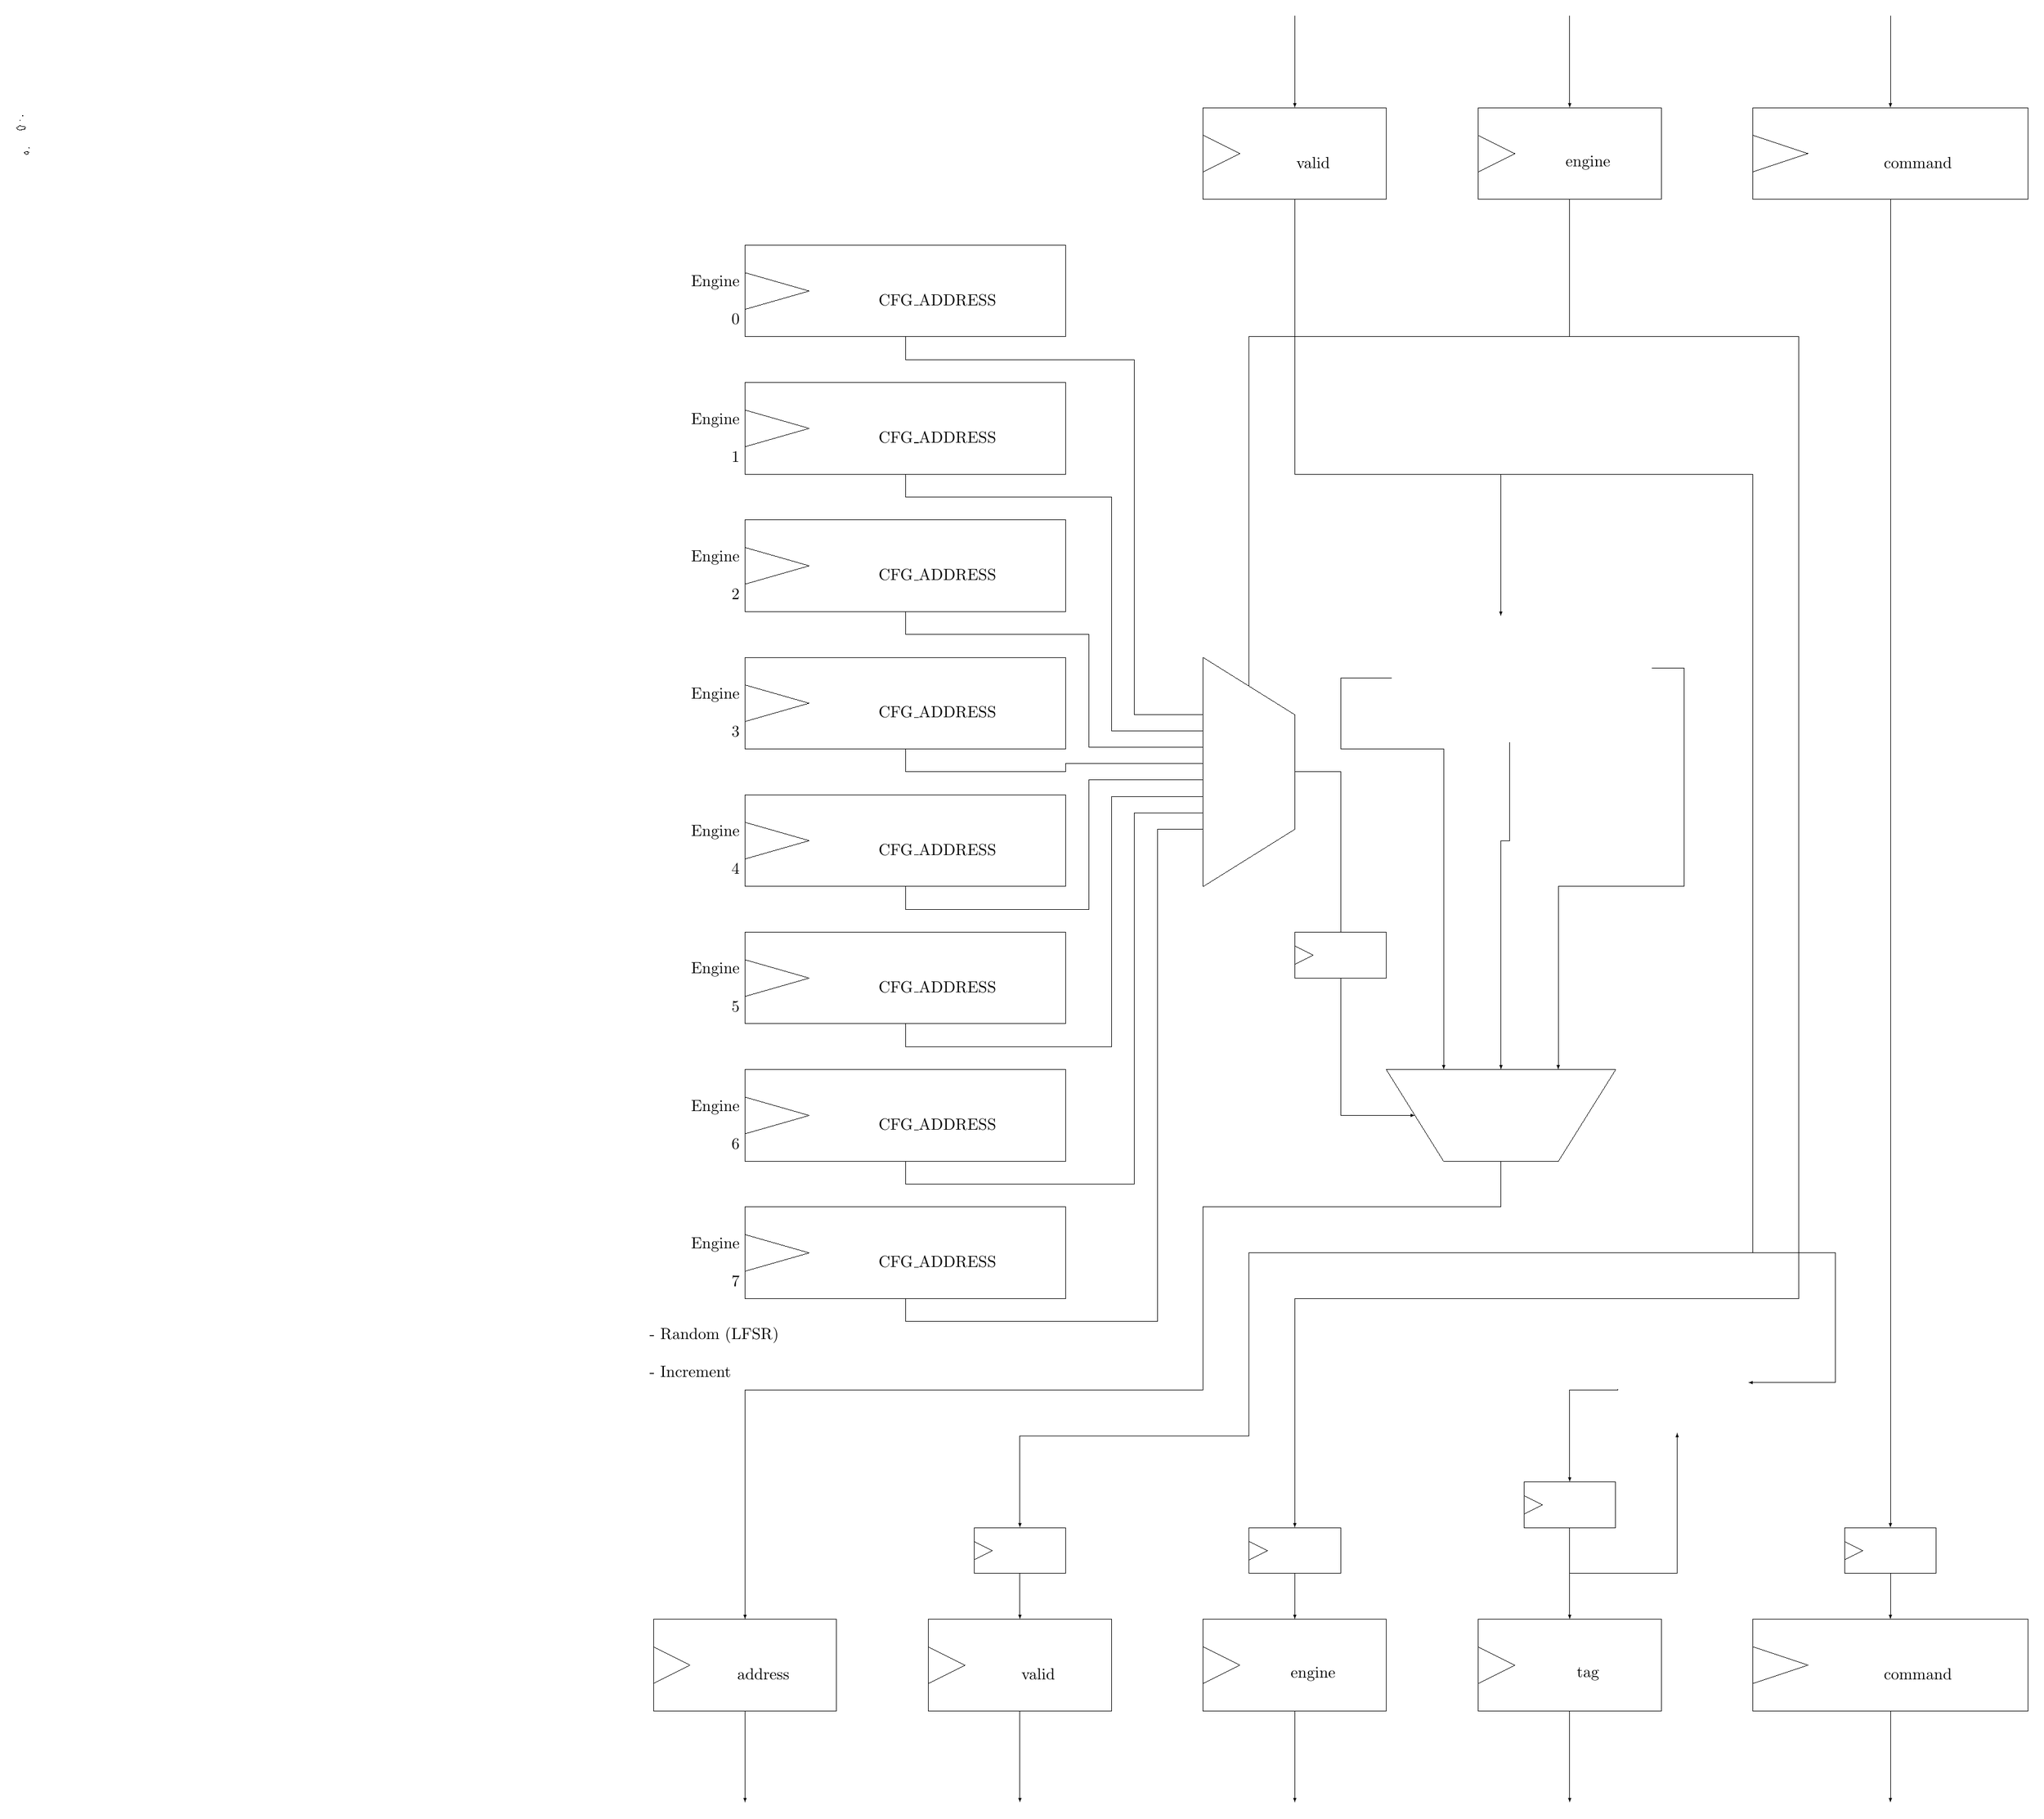
\begin{tikzpicture}
\pgftransformxscale{1.000000}
\pgftransformyscale{-1.000000}
\definecolor{dialinecolor}{rgb}{0.000000, 0.000000, 0.000000}
\pgfsetstrokecolor{dialinecolor}
\definecolor{dialinecolor}{rgb}{1.000000, 1.000000, 1.000000}
\pgfsetfillcolor{dialinecolor}
\pgfsetlinewidth{0.000000\du}
\pgfsetdash{}{0pt}
\pgfsetdash{}{0pt}
\pgfsetbuttcap
\pgfsetmiterjoin
\pgfsetlinewidth{0.000000\du}
\pgfsetbuttcap
\pgfsetmiterjoin
\pgfsetdash{}{0pt}
\definecolor{dialinecolor}{rgb}{0.000000, 0.000000, 0.000000}
\pgfsetstrokecolor{dialinecolor}
\draw (17.000000\du,3.000000\du)--(24.000000\du,3.000000\du)--(24.000000\du,5.000000\du)--(17.000000\du,5.000000\du)--cycle;
\pgfsetbuttcap
\pgfsetmiterjoin
\pgfsetdash{}{0pt}
\definecolor{dialinecolor}{rgb}{0.000000, 0.000000, 0.000000}
\pgfsetstrokecolor{dialinecolor}
\draw (17.000000\du,3.600000\du)--(18.400000\du,4.000000\du);
\pgfsetbuttcap
\pgfsetmiterjoin
\pgfsetdash{}{0pt}
\definecolor{dialinecolor}{rgb}{0.000000, 0.000000, 0.000000}
\pgfsetstrokecolor{dialinecolor}
\draw (18.400000\du,4.000000\du)--(17.000000\du,4.400000\du);
% setfont left to latex
\definecolor{dialinecolor}{rgb}{0.000000, 0.000000, 0.000000}
\pgfsetstrokecolor{dialinecolor}
\node at (21.200000\du,4.200000\du){CFG\_ADDRESS};
\pgfsetlinewidth{0.000000\du}
\pgfsetdash{}{0pt}
\pgfsetdash{}{0pt}
\pgfsetbuttcap
\pgfsetmiterjoin
\pgfsetlinewidth{0.000000\du}
\pgfsetbuttcap
\pgfsetmiterjoin
\pgfsetdash{}{0pt}
\definecolor{dialinecolor}{rgb}{0.000000, 0.000000, 0.000000}
\pgfsetstrokecolor{dialinecolor}
\draw (17.000000\du,9.000000\du)--(24.000000\du,9.000000\du)--(24.000000\du,11.000000\du)--(17.000000\du,11.000000\du)--cycle;
\pgfsetbuttcap
\pgfsetmiterjoin
\pgfsetdash{}{0pt}
\definecolor{dialinecolor}{rgb}{0.000000, 0.000000, 0.000000}
\pgfsetstrokecolor{dialinecolor}
\draw (17.000000\du,9.600000\du)--(18.400000\du,10.000000\du);
\pgfsetbuttcap
\pgfsetmiterjoin
\pgfsetdash{}{0pt}
\definecolor{dialinecolor}{rgb}{0.000000, 0.000000, 0.000000}
\pgfsetstrokecolor{dialinecolor}
\draw (18.400000\du,10.000000\du)--(17.000000\du,10.400000\du);
% setfont left to latex
\definecolor{dialinecolor}{rgb}{0.000000, 0.000000, 0.000000}
\pgfsetstrokecolor{dialinecolor}
\node at (21.200000\du,10.200000\du){CFG\_ADDRESS};
% setfont left to latex
\definecolor{dialinecolor}{rgb}{0.000000, 0.000000, 0.000000}
\pgfsetstrokecolor{dialinecolor}
\node[anchor=east] at (17.000000\du,3.821250\du){Engine };
% setfont left to latex
\definecolor{dialinecolor}{rgb}{0.000000, 0.000000, 0.000000}
\pgfsetstrokecolor{dialinecolor}
\node[anchor=east] at (17.000000\du,4.621250\du){0 };
\pgfsetlinewidth{0.000000\du}
\pgfsetdash{}{0pt}
\pgfsetdash{}{0pt}
\pgfsetbuttcap
\pgfsetmiterjoin
\pgfsetlinewidth{0.000000\du}
\pgfsetbuttcap
\pgfsetmiterjoin
\pgfsetdash{}{0pt}
\definecolor{dialinecolor}{rgb}{0.000000, 0.000000, 0.000000}
\pgfsetstrokecolor{dialinecolor}
\draw (39.000000\du,0.000000\du)--(45.000000\du,0.000000\du)--(45.000000\du,2.000000\du)--(39.000000\du,2.000000\du)--cycle;
\pgfsetbuttcap
\pgfsetmiterjoin
\pgfsetdash{}{0pt}
\definecolor{dialinecolor}{rgb}{0.000000, 0.000000, 0.000000}
\pgfsetstrokecolor{dialinecolor}
\draw (39.000000\du,0.600000\du)--(40.200000\du,1.000000\du);
\pgfsetbuttcap
\pgfsetmiterjoin
\pgfsetdash{}{0pt}
\definecolor{dialinecolor}{rgb}{0.000000, 0.000000, 0.000000}
\pgfsetstrokecolor{dialinecolor}
\draw (40.200000\du,1.000000\du)--(39.000000\du,1.400000\du);
% setfont left to latex
\definecolor{dialinecolor}{rgb}{0.000000, 0.000000, 0.000000}
\pgfsetstrokecolor{dialinecolor}
\node at (42.600000\du,1.200000\du){command};
\pgfsetlinewidth{0.000000\du}
\pgfsetdash{}{0pt}
\pgfsetdash{}{0pt}
\pgfsetbuttcap
\pgfsetmiterjoin
\pgfsetlinewidth{0.000000\du}
\pgfsetbuttcap
\pgfsetmiterjoin
\pgfsetdash{}{0pt}
\definecolor{dialinecolor}{rgb}{0.000000, 0.000000, 0.000000}
\pgfsetstrokecolor{dialinecolor}
\draw (33.000000\du,0.000000\du)--(37.000000\du,0.000000\du)--(37.000000\du,2.000000\du)--(33.000000\du,2.000000\du)--cycle;
\pgfsetbuttcap
\pgfsetmiterjoin
\pgfsetdash{}{0pt}
\definecolor{dialinecolor}{rgb}{0.000000, 0.000000, 0.000000}
\pgfsetstrokecolor{dialinecolor}
\draw (33.000000\du,0.600000\du)--(33.800000\du,1.000000\du);
\pgfsetbuttcap
\pgfsetmiterjoin
\pgfsetdash{}{0pt}
\definecolor{dialinecolor}{rgb}{0.000000, 0.000000, 0.000000}
\pgfsetstrokecolor{dialinecolor}
\draw (33.800000\du,1.000000\du)--(33.000000\du,1.400000\du);
% setfont left to latex
\definecolor{dialinecolor}{rgb}{0.000000, 0.000000, 0.000000}
\pgfsetstrokecolor{dialinecolor}
\node at (35.400000\du,1.200000\du){engine};
\pgfsetlinewidth{0.000000\du}
\pgfsetdash{}{0pt}
\pgfsetdash{}{0pt}
\pgfsetbuttcap
\pgfsetmiterjoin
\pgfsetlinewidth{0.000000\du}
\pgfsetbuttcap
\pgfsetmiterjoin
\pgfsetdash{}{0pt}
\definecolor{dialinecolor}{rgb}{0.000000, 0.000000, 0.000000}
\pgfsetstrokecolor{dialinecolor}
\draw (27.000000\du,0.000000\du)--(31.000000\du,0.000000\du)--(31.000000\du,2.000000\du)--(27.000000\du,2.000000\du)--cycle;
\pgfsetbuttcap
\pgfsetmiterjoin
\pgfsetdash{}{0pt}
\definecolor{dialinecolor}{rgb}{0.000000, 0.000000, 0.000000}
\pgfsetstrokecolor{dialinecolor}
\draw (27.000000\du,0.600000\du)--(27.800000\du,1.000000\du);
\pgfsetbuttcap
\pgfsetmiterjoin
\pgfsetdash{}{0pt}
\definecolor{dialinecolor}{rgb}{0.000000, 0.000000, 0.000000}
\pgfsetstrokecolor{dialinecolor}
\draw (27.800000\du,1.000000\du)--(27.000000\du,1.400000\du);
% setfont left to latex
\definecolor{dialinecolor}{rgb}{0.000000, 0.000000, 0.000000}
\pgfsetstrokecolor{dialinecolor}
\node at (29.400000\du,1.200000\du){valid};
\pgfsetlinewidth{0.000000\du}
\pgfsetdash{}{0pt}
\pgfsetdash{}{0pt}
\pgfsetbuttcap
{
\definecolor{dialinecolor}{rgb}{0.000000, 0.000000, 0.000000}
\pgfsetfillcolor{dialinecolor}
% was here!!!
\pgfsetarrowsend{latex}
\definecolor{dialinecolor}{rgb}{0.000000, 0.000000, 0.000000}
\pgfsetstrokecolor{dialinecolor}
\draw (42.000000\du,-2.000000\du)--(42.000000\du,0.000000\du);
}
\pgfsetlinewidth{0.000000\du}
\pgfsetdash{}{0pt}
\pgfsetdash{}{0pt}
\pgfsetbuttcap
{
\definecolor{dialinecolor}{rgb}{0.000000, 0.000000, 0.000000}
\pgfsetfillcolor{dialinecolor}
% was here!!!
\pgfsetarrowsend{latex}
\definecolor{dialinecolor}{rgb}{0.000000, 0.000000, 0.000000}
\pgfsetstrokecolor{dialinecolor}
\draw (35.000000\du,-2.000000\du)--(35.000000\du,0.000000\du);
}
\pgfsetlinewidth{0.000000\du}
\pgfsetdash{}{0pt}
\pgfsetdash{}{0pt}
\pgfsetbuttcap
{
\definecolor{dialinecolor}{rgb}{0.000000, 0.000000, 0.000000}
\pgfsetfillcolor{dialinecolor}
% was here!!!
\pgfsetarrowsend{latex}
\definecolor{dialinecolor}{rgb}{0.000000, 0.000000, 0.000000}
\pgfsetstrokecolor{dialinecolor}
\draw (29.000000\du,-2.000000\du)--(29.000000\du,0.000000\du);
}
\pgfsetlinewidth{0.000000\du}
\pgfsetdash{}{0pt}
\pgfsetdash{}{0pt}
\pgfsetbuttcap
\pgfsetmiterjoin
\pgfsetlinewidth{0.000000\du}
\pgfsetbuttcap
\pgfsetmiterjoin
\pgfsetdash{}{0pt}
\definecolor{dialinecolor}{rgb}{0.000000, 0.000000, 0.000000}
\pgfsetstrokecolor{dialinecolor}
\draw (17.000000\du,6.000000\du)--(24.000000\du,6.000000\du)--(24.000000\du,8.000000\du)--(17.000000\du,8.000000\du)--cycle;
\pgfsetbuttcap
\pgfsetmiterjoin
\pgfsetdash{}{0pt}
\definecolor{dialinecolor}{rgb}{0.000000, 0.000000, 0.000000}
\pgfsetstrokecolor{dialinecolor}
\draw (17.000000\du,6.600000\du)--(18.400000\du,7.000000\du);
\pgfsetbuttcap
\pgfsetmiterjoin
\pgfsetdash{}{0pt}
\definecolor{dialinecolor}{rgb}{0.000000, 0.000000, 0.000000}
\pgfsetstrokecolor{dialinecolor}
\draw (18.400000\du,7.000000\du)--(17.000000\du,7.400000\du);
% setfont left to latex
\definecolor{dialinecolor}{rgb}{0.000000, 0.000000, 0.000000}
\pgfsetstrokecolor{dialinecolor}
\node at (21.200000\du,7.200000\du){CFG\_ADDRESS};
\pgfsetlinewidth{0.000000\du}
\pgfsetdash{}{0pt}
\pgfsetdash{}{0pt}
\pgfsetbuttcap
\pgfsetmiterjoin
\pgfsetlinewidth{0.000000\du}
\pgfsetbuttcap
\pgfsetmiterjoin
\pgfsetdash{}{0pt}
\definecolor{dialinecolor}{rgb}{0.000000, 0.000000, 0.000000}
\pgfsetstrokecolor{dialinecolor}
\draw (17.000000\du,12.000000\du)--(24.000000\du,12.000000\du)--(24.000000\du,14.000000\du)--(17.000000\du,14.000000\du)--cycle;
\pgfsetbuttcap
\pgfsetmiterjoin
\pgfsetdash{}{0pt}
\definecolor{dialinecolor}{rgb}{0.000000, 0.000000, 0.000000}
\pgfsetstrokecolor{dialinecolor}
\draw (17.000000\du,12.600000\du)--(18.400000\du,13.000000\du);
\pgfsetbuttcap
\pgfsetmiterjoin
\pgfsetdash{}{0pt}
\definecolor{dialinecolor}{rgb}{0.000000, 0.000000, 0.000000}
\pgfsetstrokecolor{dialinecolor}
\draw (18.400000\du,13.000000\du)--(17.000000\du,13.400000\du);
% setfont left to latex
\definecolor{dialinecolor}{rgb}{0.000000, 0.000000, 0.000000}
\pgfsetstrokecolor{dialinecolor}
\node at (21.200000\du,13.200000\du){CFG\_ADDRESS};
\pgfsetlinewidth{0.000000\du}
\pgfsetdash{}{0pt}
\pgfsetdash{}{0pt}
\pgfsetbuttcap
\pgfsetmiterjoin
\pgfsetlinewidth{0.000000\du}
\pgfsetbuttcap
\pgfsetmiterjoin
\pgfsetdash{}{0pt}
\definecolor{dialinecolor}{rgb}{0.000000, 0.000000, 0.000000}
\pgfsetstrokecolor{dialinecolor}
\draw (17.000000\du,15.000000\du)--(24.000000\du,15.000000\du)--(24.000000\du,17.000000\du)--(17.000000\du,17.000000\du)--cycle;
\pgfsetbuttcap
\pgfsetmiterjoin
\pgfsetdash{}{0pt}
\definecolor{dialinecolor}{rgb}{0.000000, 0.000000, 0.000000}
\pgfsetstrokecolor{dialinecolor}
\draw (17.000000\du,15.600000\du)--(18.400000\du,16.000000\du);
\pgfsetbuttcap
\pgfsetmiterjoin
\pgfsetdash{}{0pt}
\definecolor{dialinecolor}{rgb}{0.000000, 0.000000, 0.000000}
\pgfsetstrokecolor{dialinecolor}
\draw (18.400000\du,16.000000\du)--(17.000000\du,16.400000\du);
% setfont left to latex
\definecolor{dialinecolor}{rgb}{0.000000, 0.000000, 0.000000}
\pgfsetstrokecolor{dialinecolor}
\node at (21.200000\du,16.200000\du){CFG\_ADDRESS};
\pgfsetlinewidth{0.000000\du}
\pgfsetdash{}{0pt}
\pgfsetdash{}{0pt}
\pgfsetbuttcap
\pgfsetmiterjoin
\pgfsetlinewidth{0.000000\du}
\pgfsetbuttcap
\pgfsetmiterjoin
\pgfsetdash{}{0pt}
\definecolor{dialinecolor}{rgb}{0.000000, 0.000000, 0.000000}
\pgfsetstrokecolor{dialinecolor}
\draw (17.000000\du,18.000000\du)--(24.000000\du,18.000000\du)--(24.000000\du,20.000000\du)--(17.000000\du,20.000000\du)--cycle;
\pgfsetbuttcap
\pgfsetmiterjoin
\pgfsetdash{}{0pt}
\definecolor{dialinecolor}{rgb}{0.000000, 0.000000, 0.000000}
\pgfsetstrokecolor{dialinecolor}
\draw (17.000000\du,18.600000\du)--(18.400000\du,19.000000\du);
\pgfsetbuttcap
\pgfsetmiterjoin
\pgfsetdash{}{0pt}
\definecolor{dialinecolor}{rgb}{0.000000, 0.000000, 0.000000}
\pgfsetstrokecolor{dialinecolor}
\draw (18.400000\du,19.000000\du)--(17.000000\du,19.400000\du);
% setfont left to latex
\definecolor{dialinecolor}{rgb}{0.000000, 0.000000, 0.000000}
\pgfsetstrokecolor{dialinecolor}
\node at (21.200000\du,19.200000\du){CFG\_ADDRESS};
\pgfsetlinewidth{0.000000\du}
\pgfsetdash{}{0pt}
\pgfsetdash{}{0pt}
\pgfsetbuttcap
\pgfsetmiterjoin
\pgfsetlinewidth{0.000000\du}
\pgfsetbuttcap
\pgfsetmiterjoin
\pgfsetdash{}{0pt}
\definecolor{dialinecolor}{rgb}{0.000000, 0.000000, 0.000000}
\pgfsetstrokecolor{dialinecolor}
\draw (17.000000\du,21.000000\du)--(24.000000\du,21.000000\du)--(24.000000\du,23.000000\du)--(17.000000\du,23.000000\du)--cycle;
\pgfsetbuttcap
\pgfsetmiterjoin
\pgfsetdash{}{0pt}
\definecolor{dialinecolor}{rgb}{0.000000, 0.000000, 0.000000}
\pgfsetstrokecolor{dialinecolor}
\draw (17.000000\du,21.600000\du)--(18.400000\du,22.000000\du);
\pgfsetbuttcap
\pgfsetmiterjoin
\pgfsetdash{}{0pt}
\definecolor{dialinecolor}{rgb}{0.000000, 0.000000, 0.000000}
\pgfsetstrokecolor{dialinecolor}
\draw (18.400000\du,22.000000\du)--(17.000000\du,22.400000\du);
% setfont left to latex
\definecolor{dialinecolor}{rgb}{0.000000, 0.000000, 0.000000}
\pgfsetstrokecolor{dialinecolor}
\node at (21.200000\du,22.200000\du){CFG\_ADDRESS};
\pgfsetlinewidth{0.000000\du}
\pgfsetdash{}{0pt}
\pgfsetdash{}{0pt}
\pgfsetbuttcap
\pgfsetmiterjoin
\pgfsetlinewidth{0.000000\du}
\pgfsetbuttcap
\pgfsetmiterjoin
\pgfsetdash{}{0pt}
\definecolor{dialinecolor}{rgb}{0.000000, 0.000000, 0.000000}
\pgfsetstrokecolor{dialinecolor}
\draw (17.000000\du,24.000000\du)--(24.000000\du,24.000000\du)--(24.000000\du,26.000000\du)--(17.000000\du,26.000000\du)--cycle;
\pgfsetbuttcap
\pgfsetmiterjoin
\pgfsetdash{}{0pt}
\definecolor{dialinecolor}{rgb}{0.000000, 0.000000, 0.000000}
\pgfsetstrokecolor{dialinecolor}
\draw (17.000000\du,24.600000\du)--(18.400000\du,25.000000\du);
\pgfsetbuttcap
\pgfsetmiterjoin
\pgfsetdash{}{0pt}
\definecolor{dialinecolor}{rgb}{0.000000, 0.000000, 0.000000}
\pgfsetstrokecolor{dialinecolor}
\draw (18.400000\du,25.000000\du)--(17.000000\du,25.400000\du);
% setfont left to latex
\definecolor{dialinecolor}{rgb}{0.000000, 0.000000, 0.000000}
\pgfsetstrokecolor{dialinecolor}
\node at (21.200000\du,25.200000\du){CFG\_ADDRESS};
\pgfsetlinewidth{0.000000\du}
\pgfsetdash{}{0pt}
\pgfsetdash{}{0pt}
\pgfsetbuttcap
\pgfsetmiterjoin
\pgfsetlinewidth{0.000000\du}
\pgfsetbuttcap
\pgfsetmiterjoin
\pgfsetdash{}{0pt}
\definecolor{dialinecolor}{rgb}{0.000000, 0.000000, 0.000000}
\pgfsetstrokecolor{dialinecolor}
\draw (27.000000\du,12.000000\du)--(29.000000\du,13.250000\du)--(29.000000\du,15.750000\du)--(27.000000\du,17.000000\du)--cycle;
% setfont left to latex
\definecolor{dialinecolor}{rgb}{0.000000, 0.000000, 0.000000}
\pgfsetstrokecolor{dialinecolor}
\node at (28.000000\du,14.700000\du){};
\pgfsetlinewidth{0.000000\du}
\pgfsetdash{}{0pt}
\pgfsetdash{}{0pt}
\pgfsetbuttcap
{
\definecolor{dialinecolor}{rgb}{0.000000, 0.000000, 0.000000}
\pgfsetfillcolor{dialinecolor}
% was here!!!
\definecolor{dialinecolor}{rgb}{0.000000, 0.000000, 0.000000}
\pgfsetstrokecolor{dialinecolor}
\draw (27.000000\du,13.250000\du)--(27.000000\du,15.750000\du);
}
\pgfsetlinewidth{0.000000\du}
\pgfsetdash{}{0pt}
\pgfsetdash{}{0pt}
\pgfsetmiterjoin
\pgfsetbuttcap
{
\definecolor{dialinecolor}{rgb}{0.000000, 0.000000, 0.000000}
\pgfsetfillcolor{dialinecolor}
% was here!!!
{\pgfsetcornersarced{\pgfpoint{0.000000\du}{0.000000\du}}\definecolor{dialinecolor}{rgb}{0.000000, 0.000000, 0.000000}
\pgfsetstrokecolor{dialinecolor}
\draw (20.500000\du,5.000000\du)--(20.500000\du,5.500000\du)--(25.500000\du,5.500000\du)--(25.500000\du,13.250000\du)--(27.000000\du,13.250000\du);
}}
\pgfsetlinewidth{0.000000\du}
\pgfsetdash{}{0pt}
\pgfsetdash{}{0pt}
\pgfsetmiterjoin
\pgfsetbuttcap
{
\definecolor{dialinecolor}{rgb}{0.000000, 0.000000, 0.000000}
\pgfsetfillcolor{dialinecolor}
% was here!!!
{\pgfsetcornersarced{\pgfpoint{0.000000\du}{0.000000\du}}\definecolor{dialinecolor}{rgb}{0.000000, 0.000000, 0.000000}
\pgfsetstrokecolor{dialinecolor}
\draw (20.500000\du,8.000000\du)--(20.500000\du,8.500000\du)--(25.000000\du,8.500000\du)--(25.000000\du,13.607100\du)--(27.000000\du,13.607100\du);
}}
\pgfsetlinewidth{0.000000\du}
\pgfsetdash{}{0pt}
\pgfsetdash{}{0pt}
\pgfsetmiterjoin
\pgfsetbuttcap
{
\definecolor{dialinecolor}{rgb}{0.000000, 0.000000, 0.000000}
\pgfsetfillcolor{dialinecolor}
% was here!!!
{\pgfsetcornersarced{\pgfpoint{0.000000\du}{0.000000\du}}\definecolor{dialinecolor}{rgb}{0.000000, 0.000000, 0.000000}
\pgfsetstrokecolor{dialinecolor}
\draw (20.500000\du,11.000000\du)--(20.500000\du,11.500000\du)--(24.500000\du,11.500000\du)--(24.500000\du,13.964300\du)--(27.000000\du,13.964300\du);
}}
\pgfsetlinewidth{0.000000\du}
\pgfsetdash{}{0pt}
\pgfsetdash{}{0pt}
\pgfsetmiterjoin
\pgfsetbuttcap
{
\definecolor{dialinecolor}{rgb}{0.000000, 0.000000, 0.000000}
\pgfsetfillcolor{dialinecolor}
% was here!!!
{\pgfsetcornersarced{\pgfpoint{0.000000\du}{0.000000\du}}\definecolor{dialinecolor}{rgb}{0.000000, 0.000000, 0.000000}
\pgfsetstrokecolor{dialinecolor}
\draw (20.500000\du,14.000000\du)--(20.500000\du,14.500000\du)--(24.000000\du,14.500000\du)--(24.000000\du,14.321400\du)--(27.000000\du,14.321400\du);
}}
\pgfsetlinewidth{0.000000\du}
\pgfsetdash{}{0pt}
\pgfsetdash{}{0pt}
\pgfsetmiterjoin
\pgfsetbuttcap
{
\definecolor{dialinecolor}{rgb}{0.000000, 0.000000, 0.000000}
\pgfsetfillcolor{dialinecolor}
% was here!!!
{\pgfsetcornersarced{\pgfpoint{0.000000\du}{0.000000\du}}\definecolor{dialinecolor}{rgb}{0.000000, 0.000000, 0.000000}
\pgfsetstrokecolor{dialinecolor}
\draw (20.500000\du,17.000000\du)--(20.500000\du,17.500000\du)--(24.500000\du,17.500000\du)--(24.500000\du,14.678600\du)--(27.000000\du,14.678600\du);
}}
\pgfsetlinewidth{0.000000\du}
\pgfsetdash{}{0pt}
\pgfsetdash{}{0pt}
\pgfsetmiterjoin
\pgfsetbuttcap
{
\definecolor{dialinecolor}{rgb}{0.000000, 0.000000, 0.000000}
\pgfsetfillcolor{dialinecolor}
% was here!!!
{\pgfsetcornersarced{\pgfpoint{0.000000\du}{0.000000\du}}\definecolor{dialinecolor}{rgb}{0.000000, 0.000000, 0.000000}
\pgfsetstrokecolor{dialinecolor}
\draw (20.500000\du,20.000000\du)--(20.500000\du,20.500000\du)--(25.000000\du,20.500000\du)--(25.000000\du,15.035700\du)--(27.000000\du,15.035700\du);
}}
\pgfsetlinewidth{0.000000\du}
\pgfsetdash{}{0pt}
\pgfsetdash{}{0pt}
\pgfsetmiterjoin
\pgfsetbuttcap
{
\definecolor{dialinecolor}{rgb}{0.000000, 0.000000, 0.000000}
\pgfsetfillcolor{dialinecolor}
% was here!!!
{\pgfsetcornersarced{\pgfpoint{0.000000\du}{0.000000\du}}\definecolor{dialinecolor}{rgb}{0.000000, 0.000000, 0.000000}
\pgfsetstrokecolor{dialinecolor}
\draw (20.500000\du,23.000000\du)--(20.500000\du,23.500000\du)--(25.500000\du,23.500000\du)--(25.500000\du,15.392900\du)--(27.000000\du,15.392900\du);
}}
\pgfsetlinewidth{0.000000\du}
\pgfsetdash{}{0pt}
\pgfsetdash{}{0pt}
\pgfsetmiterjoin
\pgfsetbuttcap
{
\definecolor{dialinecolor}{rgb}{0.000000, 0.000000, 0.000000}
\pgfsetfillcolor{dialinecolor}
% was here!!!
{\pgfsetcornersarced{\pgfpoint{0.000000\du}{0.000000\du}}\definecolor{dialinecolor}{rgb}{0.000000, 0.000000, 0.000000}
\pgfsetstrokecolor{dialinecolor}
\draw (20.500000\du,26.000000\du)--(20.500000\du,26.500000\du)--(26.000000\du,26.500000\du)--(26.000000\du,15.750000\du)--(27.000000\du,15.750000\du);
}}
% setfont left to latex
\definecolor{dialinecolor}{rgb}{0.000000, 0.000000, 0.000000}
\pgfsetstrokecolor{dialinecolor}
\node[anchor=east] at (17.000000\du,6.821250\du){Engine };
% setfont left to latex
\definecolor{dialinecolor}{rgb}{0.000000, 0.000000, 0.000000}
\pgfsetstrokecolor{dialinecolor}
\node[anchor=east] at (17.000000\du,7.621250\du){1 };
% setfont left to latex
\definecolor{dialinecolor}{rgb}{0.000000, 0.000000, 0.000000}
\pgfsetstrokecolor{dialinecolor}
\node[anchor=east] at (17.000000\du,9.821250\du){Engine };
% setfont left to latex
\definecolor{dialinecolor}{rgb}{0.000000, 0.000000, 0.000000}
\pgfsetstrokecolor{dialinecolor}
\node[anchor=east] at (17.000000\du,10.621250\du){2 };
% setfont left to latex
\definecolor{dialinecolor}{rgb}{0.000000, 0.000000, 0.000000}
\pgfsetstrokecolor{dialinecolor}
\node[anchor=east] at (17.000000\du,12.821250\du){Engine };
% setfont left to latex
\definecolor{dialinecolor}{rgb}{0.000000, 0.000000, 0.000000}
\pgfsetstrokecolor{dialinecolor}
\node[anchor=east] at (17.000000\du,13.621250\du){3 };
% setfont left to latex
\definecolor{dialinecolor}{rgb}{0.000000, 0.000000, 0.000000}
\pgfsetstrokecolor{dialinecolor}
\node[anchor=east] at (17.000000\du,15.821250\du){Engine };
% setfont left to latex
\definecolor{dialinecolor}{rgb}{0.000000, 0.000000, 0.000000}
\pgfsetstrokecolor{dialinecolor}
\node[anchor=east] at (17.000000\du,16.621250\du){4 };
% setfont left to latex
\definecolor{dialinecolor}{rgb}{0.000000, 0.000000, 0.000000}
\pgfsetstrokecolor{dialinecolor}
\node[anchor=east] at (17.000000\du,18.821250\du){Engine };
% setfont left to latex
\definecolor{dialinecolor}{rgb}{0.000000, 0.000000, 0.000000}
\pgfsetstrokecolor{dialinecolor}
\node[anchor=east] at (17.000000\du,19.621250\du){5 };
% setfont left to latex
\definecolor{dialinecolor}{rgb}{0.000000, 0.000000, 0.000000}
\pgfsetstrokecolor{dialinecolor}
\node[anchor=east] at (17.000000\du,21.821250\du){Engine };
% setfont left to latex
\definecolor{dialinecolor}{rgb}{0.000000, 0.000000, 0.000000}
\pgfsetstrokecolor{dialinecolor}
\node[anchor=east] at (17.000000\du,22.621250\du){6 };
% setfont left to latex
\definecolor{dialinecolor}{rgb}{0.000000, 0.000000, 0.000000}
\pgfsetstrokecolor{dialinecolor}
\node[anchor=east] at (17.000000\du,24.821250\du){Engine };
% setfont left to latex
\definecolor{dialinecolor}{rgb}{0.000000, 0.000000, 0.000000}
\pgfsetstrokecolor{dialinecolor}
\node[anchor=east] at (17.000000\du,25.621250\du){7 };
\pgfsetlinewidth{0.000000\du}
\pgfsetdash{}{0pt}
\pgfsetdash{}{0pt}
\pgfsetmiterjoin
\pgfsetbuttcap
{
\definecolor{dialinecolor}{rgb}{0.000000, 0.000000, 0.000000}
\pgfsetfillcolor{dialinecolor}
% was here!!!
{\pgfsetcornersarced{\pgfpoint{0.000000\du}{0.000000\du}}\definecolor{dialinecolor}{rgb}{0.000000, 0.000000, 0.000000}
\pgfsetstrokecolor{dialinecolor}
\draw (35.000000\du,2.000000\du)--(35.000000\du,5.000000\du)--(28.000000\du,5.000000\du)--(28.000000\du,12.625000\du);
}}
\pgfsetlinewidth{0.000000\du}
\pgfsetdash{}{0pt}
\pgfsetdash{}{0pt}
\pgfsetbuttcap
\pgfsetmiterjoin
\pgfsetlinewidth{0.000000\du}
\pgfsetbuttcap
\pgfsetmiterjoin
\pgfsetdash{}{0pt}
\definecolor{dialinecolor}{rgb}{0.000000, 0.000000, 0.000000}
\pgfsetstrokecolor{dialinecolor}
\draw (39.000000\du,33.000000\du)--(45.000000\du,33.000000\du)--(45.000000\du,35.000000\du)--(39.000000\du,35.000000\du)--cycle;
\pgfsetbuttcap
\pgfsetmiterjoin
\pgfsetdash{}{0pt}
\definecolor{dialinecolor}{rgb}{0.000000, 0.000000, 0.000000}
\pgfsetstrokecolor{dialinecolor}
\draw (39.000000\du,33.600000\du)--(40.200000\du,34.000000\du);
\pgfsetbuttcap
\pgfsetmiterjoin
\pgfsetdash{}{0pt}
\definecolor{dialinecolor}{rgb}{0.000000, 0.000000, 0.000000}
\pgfsetstrokecolor{dialinecolor}
\draw (40.200000\du,34.000000\du)--(39.000000\du,34.400000\du);
% setfont left to latex
\definecolor{dialinecolor}{rgb}{0.000000, 0.000000, 0.000000}
\pgfsetstrokecolor{dialinecolor}
\node at (42.600000\du,34.200000\du){command};
\pgfsetlinewidth{0.000000\du}
\pgfsetdash{}{0pt}
\pgfsetdash{}{0pt}
\pgfsetbuttcap
{
\definecolor{dialinecolor}{rgb}{0.000000, 0.000000, 0.000000}
\pgfsetfillcolor{dialinecolor}
% was here!!!
\pgfsetarrowsend{latex}
\definecolor{dialinecolor}{rgb}{0.000000, 0.000000, 0.000000}
\pgfsetstrokecolor{dialinecolor}
\draw (42.000000\du,35.000000\du)--(42.000000\du,37.000000\du);
}
\pgfsetlinewidth{0.000000\du}
\pgfsetdash{}{0pt}
\pgfsetdash{}{0pt}
\pgfsetbuttcap
\pgfsetmiterjoin
\pgfsetlinewidth{0.000000\du}
\pgfsetbuttcap
\pgfsetmiterjoin
\pgfsetdash{}{0pt}
\definecolor{dialinecolor}{rgb}{0.000000, 0.000000, 0.000000}
\pgfsetstrokecolor{dialinecolor}
\draw (15.000000\du,33.000000\du)--(19.000000\du,33.000000\du)--(19.000000\du,35.000000\du)--(15.000000\du,35.000000\du)--cycle;
\pgfsetbuttcap
\pgfsetmiterjoin
\pgfsetdash{}{0pt}
\definecolor{dialinecolor}{rgb}{0.000000, 0.000000, 0.000000}
\pgfsetstrokecolor{dialinecolor}
\draw (15.000000\du,33.600000\du)--(15.800000\du,34.000000\du);
\pgfsetbuttcap
\pgfsetmiterjoin
\pgfsetdash{}{0pt}
\definecolor{dialinecolor}{rgb}{0.000000, 0.000000, 0.000000}
\pgfsetstrokecolor{dialinecolor}
\draw (15.800000\du,34.000000\du)--(15.000000\du,34.400000\du);
% setfont left to latex
\definecolor{dialinecolor}{rgb}{0.000000, 0.000000, 0.000000}
\pgfsetstrokecolor{dialinecolor}
\node at (17.400000\du,34.200000\du){address};
\pgfsetlinewidth{0.000000\du}
\pgfsetdash{}{0pt}
\pgfsetdash{}{0pt}
\pgfsetbuttcap
{
\definecolor{dialinecolor}{rgb}{0.000000, 0.000000, 0.000000}
\pgfsetfillcolor{dialinecolor}
% was here!!!
\pgfsetarrowsend{latex}
\definecolor{dialinecolor}{rgb}{0.000000, 0.000000, 0.000000}
\pgfsetstrokecolor{dialinecolor}
\draw (17.000000\du,35.000000\du)--(17.000000\du,37.000000\du);
}
\pgfsetlinewidth{0.000000\du}
\pgfsetdash{}{0pt}
\pgfsetdash{}{0pt}
\pgfsetbuttcap
\pgfsetmiterjoin
\pgfsetlinewidth{0.000000\du}
\pgfsetbuttcap
\pgfsetmiterjoin
\pgfsetdash{}{0pt}
\definecolor{dialinecolor}{rgb}{1.000000, 1.000000, 1.000000}
\pgfsetfillcolor{dialinecolor}
\pgfpathmoveto{\pgfpoint{32.366199\du}{11.871624\du}}
\pgfpathcurveto{\pgfpoint{31.901409\du}{11.861488\du}}{\pgfpoint{31.000000\du}{12.074326\du}}{\pgfpoint{31.126761\du}{12.530408\du}}
\pgfpathcurveto{\pgfpoint{31.253520\du}{12.986490\du}}{\pgfpoint{31.859155\du}{13.087837\du}}{\pgfpoint{32.112677\du}{12.956084\du}}
\pgfpathcurveto{\pgfpoint{32.366199\du}{12.824327\du}}{\pgfpoint{31.718310\du}{13.594594\du}}{\pgfpoint{32.957749\du}{13.797297\du}}
\pgfpathcurveto{\pgfpoint{34.197177\du}{14.000000\du}}{\pgfpoint{34.830981\du}{13.675675\du}}{\pgfpoint{34.647882\du}{13.442567\du}}
\pgfpathcurveto{\pgfpoint{34.464783\du}{13.209459\du}}{\pgfpoint{35.732392\du}{13.989865\du}}{\pgfpoint{36.323942\du}{13.543918\du}}
\pgfpathcurveto{\pgfpoint{36.915493\du}{13.097972\du}}{\pgfpoint{35.718307\du}{12.672300\du}}{\pgfpoint{35.971829\du}{12.733111\du}}
\pgfpathcurveto{\pgfpoint{36.225350\du}{12.793922\du}}{\pgfpoint{37.000000\du}{12.712841\du}}{\pgfpoint{36.746478\du}{11.952705\du}}
\pgfpathcurveto{\pgfpoint{36.492957\du}{11.192569\du}}{\pgfpoint{34.211262\du}{11.780407\du}}{\pgfpoint{34.464783\du}{11.668921\du}}
\pgfpathcurveto{\pgfpoint{34.718305\du}{11.557434\du}}{\pgfpoint{34.084501\du}{11.000000\du}}{\pgfpoint{33.295778\du}{11.111487\du}}
\pgfpathcurveto{\pgfpoint{32.507044\du}{11.222974\du}}{\pgfpoint{32.451100\du}{11.425282\du}}{\pgfpoint{32.366593\du}{11.871228\du}}
\pgfpathlineto{\pgfpoint{32.366199\du}{11.871624\du}}
\pgfusepath{fill}
\definecolor{dialinecolor}{rgb}{0.000000, 0.000000, 0.000000}
\pgfsetstrokecolor{dialinecolor}
\pgfpathmoveto{\pgfpoint{32.366199\du}{11.871624\du}}
\pgfpathcurveto{\pgfpoint{31.901409\du}{11.861488\du}}{\pgfpoint{31.000000\du}{12.074326\du}}{\pgfpoint{31.126761\du}{12.530408\du}}
\pgfpathcurveto{\pgfpoint{31.253520\du}{12.986490\du}}{\pgfpoint{31.859155\du}{13.087837\du}}{\pgfpoint{32.112677\du}{12.956084\du}}
\pgfpathcurveto{\pgfpoint{32.366199\du}{12.824327\du}}{\pgfpoint{31.718310\du}{13.594594\du}}{\pgfpoint{32.957749\du}{13.797297\du}}
\pgfpathcurveto{\pgfpoint{34.197177\du}{14.000000\du}}{\pgfpoint{34.830981\du}{13.675675\du}}{\pgfpoint{34.647882\du}{13.442567\du}}
\pgfpathcurveto{\pgfpoint{34.464783\du}{13.209459\du}}{\pgfpoint{35.732392\du}{13.989865\du}}{\pgfpoint{36.323942\du}{13.543918\du}}
\pgfpathcurveto{\pgfpoint{36.915493\du}{13.097972\du}}{\pgfpoint{35.718307\du}{12.672300\du}}{\pgfpoint{35.971829\du}{12.733111\du}}
\pgfpathcurveto{\pgfpoint{36.225350\du}{12.793922\du}}{\pgfpoint{37.000000\du}{12.712841\du}}{\pgfpoint{36.746478\du}{11.952705\du}}
\pgfpathcurveto{\pgfpoint{36.492957\du}{11.192569\du}}{\pgfpoint{34.211262\du}{11.780407\du}}{\pgfpoint{34.464783\du}{11.668921\du}}
\pgfpathcurveto{\pgfpoint{34.718305\du}{11.557434\du}}{\pgfpoint{34.084501\du}{11.000000\du}}{\pgfpoint{33.295778\du}{11.111487\du}}
\pgfpathcurveto{\pgfpoint{32.507044\du}{11.222974\du}}{\pgfpoint{32.451100\du}{11.425282\du}}{\pgfpoint{32.366593\du}{11.871228\du}}
\pgfpathlineto{\pgfpoint{32.366199\du}{11.871624\du}}
\pgfusepath{stroke}
% setfont left to latex
\definecolor{dialinecolor}{rgb}{0.000000, 0.000000, 0.000000}
\pgfsetstrokecolor{dialinecolor}
\node at (34.160839\du,12.752884\du){};
\pgfsetlinewidth{0.000000\du}
\pgfsetdash{}{0pt}
\pgfsetdash{}{0pt}
\pgfsetmiterjoin
\pgfsetbuttcap
{
\definecolor{dialinecolor}{rgb}{0.000000, 0.000000, 0.000000}
\pgfsetfillcolor{dialinecolor}
% was here!!!
\pgfsetarrowsend{latex}
{\pgfsetcornersarced{\pgfpoint{0.000000\du}{0.000000\du}}\definecolor{dialinecolor}{rgb}{0.000000, 0.000000, 0.000000}
\pgfsetstrokecolor{dialinecolor}
\draw (29.000000\du,2.000000\du)--(29.000000\du,8.000000\du)--(33.496300\du,8.000000\du)--(33.496300\du,11.097800\du);
}}
\pgfsetlinewidth{0.000000\du}
\pgfsetdash{}{0pt}
\pgfsetdash{}{0pt}
\pgfsetbuttcap
\pgfsetmiterjoin
\pgfsetlinewidth{0.000000\du}
\pgfsetbuttcap
\pgfsetmiterjoin
\pgfsetdash{}{0pt}
\definecolor{dialinecolor}{rgb}{0.000000, 0.000000, 0.000000}
\pgfsetstrokecolor{dialinecolor}
\draw (31.000000\du,21.000000\du)--(36.000000\du,21.000000\du)--(34.750000\du,23.000000\du)--(32.250000\du,23.000000\du)--cycle;
% setfont left to latex
\definecolor{dialinecolor}{rgb}{0.000000, 0.000000, 0.000000}
\pgfsetstrokecolor{dialinecolor}
\node at (33.500000\du,22.200000\du){};
\pgfsetlinewidth{0.000000\du}
\pgfsetdash{}{0pt}
\pgfsetdash{}{0pt}
\pgfsetmiterjoin
\pgfsetbuttcap
{
\definecolor{dialinecolor}{rgb}{0.000000, 0.000000, 0.000000}
\pgfsetfillcolor{dialinecolor}
% was here!!!
{\pgfsetcornersarced{\pgfpoint{0.000000\du}{0.000000\du}}\definecolor{dialinecolor}{rgb}{0.000000, 0.000000, 0.000000}
\pgfsetstrokecolor{dialinecolor}
\draw (29.000000\du,14.500000\du)--(30.000000\du,14.500000\du)--(30.000000\du,18.000000\du)--(30.000000\du,18.000000\du);
}}
\pgfsetlinewidth{0.000000\du}
\pgfsetdash{}{0pt}
\pgfsetdash{}{0pt}
\pgfsetmiterjoin
\pgfsetbuttcap
{
\definecolor{dialinecolor}{rgb}{0.000000, 0.000000, 0.000000}
\pgfsetfillcolor{dialinecolor}
% was here!!!
\pgfsetarrowsend{latex}
{\pgfsetcornersarced{\pgfpoint{0.000000\du}{0.000000\du}}\definecolor{dialinecolor}{rgb}{0.000000, 0.000000, 0.000000}
\pgfsetstrokecolor{dialinecolor}
\draw (33.500000\du,23.000000\du)--(33.500000\du,24.000000\du)--(27.000000\du,24.000000\du)--(27.000000\du,28.000000\du)--(17.000000\du,28.000000\du)--(17.000000\du,33.000000\du);
}}
\pgfsetlinewidth{0.000000\du}
\pgfsetdash{}{0pt}
\pgfsetdash{}{0pt}
\pgfsetbuttcap
\pgfsetmiterjoin
\pgfsetlinewidth{0.000000\du}
\pgfsetbuttcap
\pgfsetmiterjoin
\pgfsetdash{}{0pt}
\definecolor{dialinecolor}{rgb}{0.000000, 0.000000, 0.000000}
\pgfsetstrokecolor{dialinecolor}
\draw (29.000000\du,18.000000\du)--(31.000000\du,18.000000\du)--(31.000000\du,19.000000\du)--(29.000000\du,19.000000\du)--cycle;
\pgfsetbuttcap
\pgfsetmiterjoin
\pgfsetdash{}{0pt}
\definecolor{dialinecolor}{rgb}{0.000000, 0.000000, 0.000000}
\pgfsetstrokecolor{dialinecolor}
\draw (29.000000\du,18.300000\du)--(29.400000\du,18.500000\du);
\pgfsetbuttcap
\pgfsetmiterjoin
\pgfsetdash{}{0pt}
\definecolor{dialinecolor}{rgb}{0.000000, 0.000000, 0.000000}
\pgfsetstrokecolor{dialinecolor}
\draw (29.400000\du,18.500000\du)--(29.000000\du,18.700000\du);
% setfont left to latex
\definecolor{dialinecolor}{rgb}{0.000000, 0.000000, 0.000000}
\pgfsetstrokecolor{dialinecolor}
\node at (30.200000\du,18.700000\du){};
\pgfsetlinewidth{0.000000\du}
\pgfsetdash{}{0pt}
\pgfsetdash{}{0pt}
\pgfsetmiterjoin
\pgfsetbuttcap
{
\definecolor{dialinecolor}{rgb}{0.000000, 0.000000, 0.000000}
\pgfsetfillcolor{dialinecolor}
% was here!!!
\pgfsetarrowsend{latex}
{\pgfsetcornersarced{\pgfpoint{0.000000\du}{0.000000\du}}\definecolor{dialinecolor}{rgb}{0.000000, 0.000000, 0.000000}
\pgfsetstrokecolor{dialinecolor}
\draw (30.000000\du,19.000000\du)--(30.000000\du,19.000000\du)--(30.000000\du,22.000000\du)--(31.625000\du,22.000000\du);
}}
\pgfsetlinewidth{0.000000\du}
\pgfsetdash{}{0pt}
\pgfsetdash{}{0pt}
\pgfsetbuttcap
\pgfsetmiterjoin
\pgfsetlinewidth{0.000000\du}
\pgfsetbuttcap
\pgfsetmiterjoin
\pgfsetdash{}{0pt}
\definecolor{dialinecolor}{rgb}{0.000000, 0.000000, 0.000000}
\pgfsetstrokecolor{dialinecolor}
\draw (41.000000\du,31.000000\du)--(43.000000\du,31.000000\du)--(43.000000\du,32.000000\du)--(41.000000\du,32.000000\du)--cycle;
\pgfsetbuttcap
\pgfsetmiterjoin
\pgfsetdash{}{0pt}
\definecolor{dialinecolor}{rgb}{0.000000, 0.000000, 0.000000}
\pgfsetstrokecolor{dialinecolor}
\draw (41.000000\du,31.300000\du)--(41.400000\du,31.500000\du);
\pgfsetbuttcap
\pgfsetmiterjoin
\pgfsetdash{}{0pt}
\definecolor{dialinecolor}{rgb}{0.000000, 0.000000, 0.000000}
\pgfsetstrokecolor{dialinecolor}
\draw (41.400000\du,31.500000\du)--(41.000000\du,31.700000\du);
% setfont left to latex
\definecolor{dialinecolor}{rgb}{0.000000, 0.000000, 0.000000}
\pgfsetstrokecolor{dialinecolor}
\node at (42.200000\du,31.700000\du){};
\pgfsetlinewidth{0.000000\du}
\pgfsetdash{}{0pt}
\pgfsetdash{}{0pt}
\pgfsetmiterjoin
\pgfsetbuttcap
{
\definecolor{dialinecolor}{rgb}{0.000000, 0.000000, 0.000000}
\pgfsetfillcolor{dialinecolor}
% was here!!!
\pgfsetarrowsend{latex}
{\pgfsetcornersarced{\pgfpoint{0.000000\du}{0.000000\du}}\definecolor{dialinecolor}{rgb}{0.000000, 0.000000, 0.000000}
\pgfsetstrokecolor{dialinecolor}
\draw (42.000000\du,2.000000\du)--(42.000000\du,27.000000\du)--(42.000000\du,27.000000\du)--(42.000000\du,31.000000\du);
}}
\pgfsetlinewidth{0.000000\du}
\pgfsetdash{}{0pt}
\pgfsetdash{}{0pt}
\pgfsetbuttcap
\pgfsetmiterjoin
\pgfsetlinewidth{0.000000\du}
\pgfsetbuttcap
\pgfsetmiterjoin
\pgfsetdash{}{0pt}
\definecolor{dialinecolor}{rgb}{0.000000, 0.000000, 0.000000}
\pgfsetstrokecolor{dialinecolor}
\draw (27.000000\du,33.000000\du)--(31.000000\du,33.000000\du)--(31.000000\du,35.000000\du)--(27.000000\du,35.000000\du)--cycle;
\pgfsetbuttcap
\pgfsetmiterjoin
\pgfsetdash{}{0pt}
\definecolor{dialinecolor}{rgb}{0.000000, 0.000000, 0.000000}
\pgfsetstrokecolor{dialinecolor}
\draw (27.000000\du,33.600000\du)--(27.800000\du,34.000000\du);
\pgfsetbuttcap
\pgfsetmiterjoin
\pgfsetdash{}{0pt}
\definecolor{dialinecolor}{rgb}{0.000000, 0.000000, 0.000000}
\pgfsetstrokecolor{dialinecolor}
\draw (27.800000\du,34.000000\du)--(27.000000\du,34.400000\du);
% setfont left to latex
\definecolor{dialinecolor}{rgb}{0.000000, 0.000000, 0.000000}
\pgfsetstrokecolor{dialinecolor}
\node at (29.400000\du,34.200000\du){engine};
\pgfsetlinewidth{0.000000\du}
\pgfsetdash{}{0pt}
\pgfsetdash{}{0pt}
\pgfsetbuttcap
\pgfsetmiterjoin
\pgfsetlinewidth{0.000000\du}
\pgfsetbuttcap
\pgfsetmiterjoin
\pgfsetdash{}{0pt}
\definecolor{dialinecolor}{rgb}{0.000000, 0.000000, 0.000000}
\pgfsetstrokecolor{dialinecolor}
\draw (21.000000\du,33.000000\du)--(25.000000\du,33.000000\du)--(25.000000\du,35.000000\du)--(21.000000\du,35.000000\du)--cycle;
\pgfsetbuttcap
\pgfsetmiterjoin
\pgfsetdash{}{0pt}
\definecolor{dialinecolor}{rgb}{0.000000, 0.000000, 0.000000}
\pgfsetstrokecolor{dialinecolor}
\draw (21.000000\du,33.600000\du)--(21.800000\du,34.000000\du);
\pgfsetbuttcap
\pgfsetmiterjoin
\pgfsetdash{}{0pt}
\definecolor{dialinecolor}{rgb}{0.000000, 0.000000, 0.000000}
\pgfsetstrokecolor{dialinecolor}
\draw (21.800000\du,34.000000\du)--(21.000000\du,34.400000\du);
% setfont left to latex
\definecolor{dialinecolor}{rgb}{0.000000, 0.000000, 0.000000}
\pgfsetstrokecolor{dialinecolor}
\node at (23.400000\du,34.200000\du){valid};
\pgfsetlinewidth{0.000000\du}
\pgfsetdash{}{0pt}
\pgfsetdash{}{0pt}
\pgfsetbuttcap
{
\definecolor{dialinecolor}{rgb}{0.000000, 0.000000, 0.000000}
\pgfsetfillcolor{dialinecolor}
% was here!!!
\pgfsetarrowsend{latex}
\definecolor{dialinecolor}{rgb}{0.000000, 0.000000, 0.000000}
\pgfsetstrokecolor{dialinecolor}
\draw (23.000000\du,32.000000\du)--(23.000000\du,33.000000\du);
}
\pgfsetlinewidth{0.000000\du}
\pgfsetdash{}{0pt}
\pgfsetdash{}{0pt}
\pgfsetbuttcap
\pgfsetmiterjoin
\pgfsetlinewidth{0.000000\du}
\pgfsetbuttcap
\pgfsetmiterjoin
\pgfsetdash{}{0pt}
\definecolor{dialinecolor}{rgb}{0.000000, 0.000000, 0.000000}
\pgfsetstrokecolor{dialinecolor}
\draw (22.000000\du,31.000000\du)--(24.000000\du,31.000000\du)--(24.000000\du,32.000000\du)--(22.000000\du,32.000000\du)--cycle;
\pgfsetbuttcap
\pgfsetmiterjoin
\pgfsetdash{}{0pt}
\definecolor{dialinecolor}{rgb}{0.000000, 0.000000, 0.000000}
\pgfsetstrokecolor{dialinecolor}
\draw (22.000000\du,31.300000\du)--(22.400000\du,31.500000\du);
\pgfsetbuttcap
\pgfsetmiterjoin
\pgfsetdash{}{0pt}
\definecolor{dialinecolor}{rgb}{0.000000, 0.000000, 0.000000}
\pgfsetstrokecolor{dialinecolor}
\draw (22.400000\du,31.500000\du)--(22.000000\du,31.700000\du);
% setfont left to latex
\definecolor{dialinecolor}{rgb}{0.000000, 0.000000, 0.000000}
\pgfsetstrokecolor{dialinecolor}
\node at (23.200000\du,31.700000\du){};
\pgfsetlinewidth{0.000000\du}
\pgfsetdash{}{0pt}
\pgfsetdash{}{0pt}
\pgfsetbuttcap
\pgfsetmiterjoin
\pgfsetlinewidth{0.000000\du}
\pgfsetbuttcap
\pgfsetmiterjoin
\pgfsetdash{}{0pt}
\definecolor{dialinecolor}{rgb}{0.000000, 0.000000, 0.000000}
\pgfsetstrokecolor{dialinecolor}
\draw (28.000000\du,31.000000\du)--(30.000000\du,31.000000\du)--(30.000000\du,32.000000\du)--(28.000000\du,32.000000\du)--cycle;
\pgfsetbuttcap
\pgfsetmiterjoin
\pgfsetdash{}{0pt}
\definecolor{dialinecolor}{rgb}{0.000000, 0.000000, 0.000000}
\pgfsetstrokecolor{dialinecolor}
\draw (28.000000\du,31.300000\du)--(28.400000\du,31.500000\du);
\pgfsetbuttcap
\pgfsetmiterjoin
\pgfsetdash{}{0pt}
\definecolor{dialinecolor}{rgb}{0.000000, 0.000000, 0.000000}
\pgfsetstrokecolor{dialinecolor}
\draw (28.400000\du,31.500000\du)--(28.000000\du,31.700000\du);
% setfont left to latex
\definecolor{dialinecolor}{rgb}{0.000000, 0.000000, 0.000000}
\pgfsetstrokecolor{dialinecolor}
\node at (29.200000\du,31.700000\du){};
\pgfsetlinewidth{0.000000\du}
\pgfsetdash{}{0pt}
\pgfsetdash{}{0pt}
\pgfsetmiterjoin
\pgfsetbuttcap
{
\definecolor{dialinecolor}{rgb}{0.000000, 0.000000, 0.000000}
\pgfsetfillcolor{dialinecolor}
% was here!!!
\pgfsetarrowsend{latex}
{\pgfsetcornersarced{\pgfpoint{0.000000\du}{0.000000\du}}\definecolor{dialinecolor}{rgb}{0.000000, 0.000000, 0.000000}
\pgfsetstrokecolor{dialinecolor}
\draw (35.000000\du,2.000000\du)--(35.000000\du,2.000000\du)--(35.000000\du,5.000000\du)--(40.000000\du,5.000000\du)--(40.000000\du,26.000000\du)--(29.000000\du,26.000000\du)--(29.000000\du,31.000000\du);
}}
\pgfsetlinewidth{0.000000\du}
\pgfsetdash{}{0pt}
\pgfsetdash{}{0pt}
\pgfsetmiterjoin
\pgfsetbuttcap
{
\definecolor{dialinecolor}{rgb}{0.000000, 0.000000, 0.000000}
\pgfsetfillcolor{dialinecolor}
% was here!!!
\pgfsetarrowsend{latex}
{\pgfsetcornersarced{\pgfpoint{0.000000\du}{0.000000\du}}\definecolor{dialinecolor}{rgb}{0.000000, 0.000000, 0.000000}
\pgfsetstrokecolor{dialinecolor}
\draw (29.000000\du,2.000000\du)--(29.000000\du,2.000000\du)--(29.000000\du,8.000000\du)--(39.000000\du,8.000000\du)--(39.000000\du,25.000000\du)--(28.000000\du,25.000000\du)--(28.000000\du,29.000000\du)--(23.000000\du,29.000000\du)--(23.000000\du,31.000000\du);
}}
\pgfsetlinewidth{0.000000\du}
\pgfsetdash{}{0pt}
\pgfsetdash{}{0pt}
\pgfsetbuttcap
\pgfsetmiterjoin
\pgfsetlinewidth{0.000000\du}
\pgfsetbuttcap
\pgfsetmiterjoin
\pgfsetdash{}{0pt}
\pgfsetbuttcap
\pgfsetmiterjoin
\pgfsetdash{}{0pt}
\definecolor{dialinecolor}{rgb}{0.000000, 0.000000, 0.000000}
\pgfsetfillcolor{dialinecolor}
\pgfpathellipse{\pgfpoint{33.500000\du}{8.000000\du}}{\pgfpoint{0.125000\du}{0\du}}{\pgfpoint{0\du}{0.125000\du}}
\pgfusepath{fill}
\definecolor{dialinecolor}{rgb}{0.000000, 0.000000, 0.000000}
\pgfsetstrokecolor{dialinecolor}
\pgfpathellipse{\pgfpoint{33.500000\du}{8.000000\du}}{\pgfpoint{0.125000\du}{0\du}}{\pgfpoint{0\du}{0.125000\du}}
\pgfusepath{stroke}
\pgfsetlinewidth{0.000000\du}
\pgfsetdash{}{0pt}
\pgfsetdash{}{0pt}
\pgfsetbuttcap
{
\definecolor{dialinecolor}{rgb}{0.000000, 0.000000, 0.000000}
\pgfsetfillcolor{dialinecolor}
% was here!!!
\definecolor{dialinecolor}{rgb}{0.000000, 0.000000, 0.000000}
\pgfsetstrokecolor{dialinecolor}
\draw (32.250000\du,21.000000\du)--(34.750000\du,21.000000\du);
}
\pgfsetlinewidth{0.000000\du}
\pgfsetdash{}{0pt}
\pgfsetdash{}{0pt}
\pgfsetmiterjoin
\pgfsetbuttcap
{
\definecolor{dialinecolor}{rgb}{0.000000, 0.000000, 0.000000}
\pgfsetfillcolor{dialinecolor}
% was here!!!
\pgfsetarrowsend{latex}
{\pgfsetcornersarced{\pgfpoint{0.000000\du}{0.000000\du}}\definecolor{dialinecolor}{rgb}{0.000000, 0.000000, 0.000000}
\pgfsetstrokecolor{dialinecolor}
\draw (31.112000\du,12.455600\du)--(30.000000\du,12.455600\du)--(30.000000\du,14.000000\du)--(32.250000\du,14.000000\du)--(32.250000\du,21.000000\du);
}}
\pgfsetlinewidth{0.000000\du}
\pgfsetdash{}{0pt}
\pgfsetdash{}{0pt}
\pgfsetmiterjoin
\pgfsetbuttcap
{
\definecolor{dialinecolor}{rgb}{0.000000, 0.000000, 0.000000}
\pgfsetfillcolor{dialinecolor}
% was here!!!
\pgfsetarrowsend{latex}
{\pgfsetcornersarced{\pgfpoint{0.000000\du}{0.000000\du}}\definecolor{dialinecolor}{rgb}{0.000000, 0.000000, 0.000000}
\pgfsetstrokecolor{dialinecolor}
\draw (36.794100\du,12.237700\du)--(37.500000\du,12.237700\du)--(37.500000\du,17.000000\du)--(34.750000\du,17.000000\du)--(34.750000\du,21.000000\du);
}}
\pgfsetlinewidth{0.000000\du}
\pgfsetdash{}{0pt}
\pgfsetdash{}{0pt}
\pgfsetmiterjoin
\pgfsetbuttcap
{
\definecolor{dialinecolor}{rgb}{0.000000, 0.000000, 0.000000}
\pgfsetfillcolor{dialinecolor}
% was here!!!
\pgfsetarrowsend{latex}
{\pgfsetcornersarced{\pgfpoint{0.000000\du}{0.000000\du}}\definecolor{dialinecolor}{rgb}{0.000000, 0.000000, 0.000000}
\pgfsetstrokecolor{dialinecolor}
\draw (33.692500\du,13.862500\du)--(33.692500\du,16.000000\du)--(33.500000\du,16.000000\du)--(33.500000\du,21.000000\du);
}}
% setfont left to latex
\definecolor{dialinecolor}{rgb}{0.000000, 0.000000, 0.000000}
\pgfsetstrokecolor{dialinecolor}
\node[anchor=west] at (14.800000\du,26.800000\du){- Random (LFSR)};
% setfont left to latex
\definecolor{dialinecolor}{rgb}{0.000000, 0.000000, 0.000000}
\pgfsetstrokecolor{dialinecolor}
\node[anchor=west] at (14.800000\du,27.600000\du){- Increment};
\pgfsetlinewidth{0.000000\du}
\pgfsetdash{}{0pt}
\pgfsetdash{}{0pt}
\pgfsetbuttcap
{
\definecolor{dialinecolor}{rgb}{0.000000, 0.000000, 0.000000}
\pgfsetfillcolor{dialinecolor}
% was here!!!
\pgfsetarrowsend{latex}
\definecolor{dialinecolor}{rgb}{0.000000, 0.000000, 0.000000}
\pgfsetstrokecolor{dialinecolor}
\draw (23.000000\du,35.000000\du)--(23.000000\du,37.000000\du);
}
\pgfsetlinewidth{0.000000\du}
\pgfsetdash{}{0pt}
\pgfsetdash{}{0pt}
\pgfsetbuttcap
{
\definecolor{dialinecolor}{rgb}{0.000000, 0.000000, 0.000000}
\pgfsetfillcolor{dialinecolor}
% was here!!!
\pgfsetarrowsend{latex}
\definecolor{dialinecolor}{rgb}{0.000000, 0.000000, 0.000000}
\pgfsetstrokecolor{dialinecolor}
\draw (29.000000\du,35.000000\du)--(29.000000\du,37.000000\du);
}
\pgfsetlinewidth{0.000000\du}
\pgfsetdash{}{0pt}
\pgfsetdash{}{0pt}
\pgfsetbuttcap
\pgfsetmiterjoin
\pgfsetlinewidth{0.000000\du}
\pgfsetbuttcap
\pgfsetmiterjoin
\pgfsetdash{}{0pt}
\pgfsetbuttcap
\pgfsetmiterjoin
\pgfsetdash{}{0pt}
\definecolor{dialinecolor}{rgb}{0.000000, 0.000000, 0.000000}
\pgfsetfillcolor{dialinecolor}
\pgfpathellipse{\pgfpoint{35.000000\du}{5.000000\du}}{\pgfpoint{0.125000\du}{0\du}}{\pgfpoint{0\du}{0.125000\du}}
\pgfusepath{fill}
\definecolor{dialinecolor}{rgb}{0.000000, 0.000000, 0.000000}
\pgfsetstrokecolor{dialinecolor}
\pgfpathellipse{\pgfpoint{35.000000\du}{5.000000\du}}{\pgfpoint{0.125000\du}{0\du}}{\pgfpoint{0\du}{0.125000\du}}
\pgfusepath{stroke}
\pgfsetlinewidth{0.000000\du}
\pgfsetdash{}{0pt}
\pgfsetdash{}{0pt}
\pgfsetbuttcap
{
\definecolor{dialinecolor}{rgb}{0.000000, 0.000000, 0.000000}
\pgfsetfillcolor{dialinecolor}
% was here!!!
\pgfsetarrowsend{latex}
\definecolor{dialinecolor}{rgb}{0.000000, 0.000000, 0.000000}
\pgfsetstrokecolor{dialinecolor}
\draw (29.000000\du,32.000000\du)--(29.000000\du,33.000000\du);
}
\pgfsetlinewidth{0.000000\du}
\pgfsetdash{}{0pt}
\pgfsetdash{}{0pt}
\pgfsetbuttcap
{
\definecolor{dialinecolor}{rgb}{0.000000, 0.000000, 0.000000}
\pgfsetfillcolor{dialinecolor}
% was here!!!
\pgfsetarrowsend{latex}
\definecolor{dialinecolor}{rgb}{0.000000, 0.000000, 0.000000}
\pgfsetstrokecolor{dialinecolor}
\draw (42.000000\du,32.000000\du)--(42.000000\du,33.000000\du);
}
\pgfsetlinewidth{0.000000\du}
\pgfsetdash{}{0pt}
\pgfsetdash{}{0pt}
\pgfsetbuttcap
\pgfsetmiterjoin
\pgfsetlinewidth{0.000000\du}
\pgfsetbuttcap
\pgfsetmiterjoin
\pgfsetdash{}{0pt}
\definecolor{dialinecolor}{rgb}{0.000000, 0.000000, 0.000000}
\pgfsetstrokecolor{dialinecolor}
\draw (33.000000\du,33.000000\du)--(37.000000\du,33.000000\du)--(37.000000\du,35.000000\du)--(33.000000\du,35.000000\du)--cycle;
\pgfsetbuttcap
\pgfsetmiterjoin
\pgfsetdash{}{0pt}
\definecolor{dialinecolor}{rgb}{0.000000, 0.000000, 0.000000}
\pgfsetstrokecolor{dialinecolor}
\draw (33.000000\du,33.600000\du)--(33.800000\du,34.000000\du);
\pgfsetbuttcap
\pgfsetmiterjoin
\pgfsetdash{}{0pt}
\definecolor{dialinecolor}{rgb}{0.000000, 0.000000, 0.000000}
\pgfsetstrokecolor{dialinecolor}
\draw (33.800000\du,34.000000\du)--(33.000000\du,34.400000\du);
% setfont left to latex
\definecolor{dialinecolor}{rgb}{0.000000, 0.000000, 0.000000}
\pgfsetstrokecolor{dialinecolor}
\node at (35.400000\du,34.200000\du){tag};
\pgfsetlinewidth{0.000000\du}
\pgfsetdash{}{0pt}
\pgfsetdash{}{0pt}
\pgfsetbuttcap
{
\definecolor{dialinecolor}{rgb}{0.000000, 0.000000, 0.000000}
\pgfsetfillcolor{dialinecolor}
% was here!!!
\pgfsetarrowsend{latex}
\definecolor{dialinecolor}{rgb}{0.000000, 0.000000, 0.000000}
\pgfsetstrokecolor{dialinecolor}
\draw (35.000000\du,35.000000\du)--(35.000000\du,37.000000\du);
}
\pgfsetlinewidth{0.000000\du}
\pgfsetdash{}{0pt}
\pgfsetdash{}{0pt}
\pgfsetbuttcap
\pgfsetmiterjoin
\pgfsetlinewidth{0.000000\du}
\pgfsetbuttcap
\pgfsetmiterjoin
\pgfsetdash{}{0pt}
\definecolor{dialinecolor}{rgb}{0.000000, 0.000000, 0.000000}
\pgfsetstrokecolor{dialinecolor}
\draw (34.000000\du,30.000000\du)--(36.000000\du,30.000000\du)--(36.000000\du,31.000000\du)--(34.000000\du,31.000000\du)--cycle;
\pgfsetbuttcap
\pgfsetmiterjoin
\pgfsetdash{}{0pt}
\definecolor{dialinecolor}{rgb}{0.000000, 0.000000, 0.000000}
\pgfsetstrokecolor{dialinecolor}
\draw (34.000000\du,30.300000\du)--(34.400000\du,30.500000\du);
\pgfsetbuttcap
\pgfsetmiterjoin
\pgfsetdash{}{0pt}
\definecolor{dialinecolor}{rgb}{0.000000, 0.000000, 0.000000}
\pgfsetstrokecolor{dialinecolor}
\draw (34.400000\du,30.500000\du)--(34.000000\du,30.700000\du);
% setfont left to latex
\definecolor{dialinecolor}{rgb}{0.000000, 0.000000, 0.000000}
\pgfsetstrokecolor{dialinecolor}
\node at (35.200000\du,30.700000\du){};
\pgfsetlinewidth{0.000000\du}
\pgfsetdash{}{0pt}
\pgfsetdash{}{0pt}
\pgfsetbuttcap
{
\definecolor{dialinecolor}{rgb}{0.000000, 0.000000, 0.000000}
\pgfsetfillcolor{dialinecolor}
% was here!!!
\pgfsetarrowsend{latex}
\definecolor{dialinecolor}{rgb}{0.000000, 0.000000, 0.000000}
\pgfsetstrokecolor{dialinecolor}
\draw (35.000000\du,31.000000\du)--(35.000000\du,33.000000\du);
}
\pgfsetlinewidth{0.000000\du}
\pgfsetdash{}{0pt}
\pgfsetdash{}{0pt}
\pgfsetbuttcap
\pgfsetmiterjoin
\pgfsetlinewidth{0.000000\du}
\pgfsetbuttcap
\pgfsetmiterjoin
\pgfsetdash{}{0pt}
\definecolor{dialinecolor}{rgb}{1.000000, 1.000000, 1.000000}
\pgfsetfillcolor{dialinecolor}
\pgfpathmoveto{\pgfpoint{36.683099\du}{27.586631\du}}
\pgfpathcurveto{\pgfpoint{36.450704\du}{27.579810\du}}{\pgfpoint{36.000000\du}{27.723057\du}}{\pgfpoint{36.063380\du}{28.030014\du}}
\pgfpathcurveto{\pgfpoint{36.126760\du}{28.336972\du}}{\pgfpoint{36.429578\du}{28.405182\du}}{\pgfpoint{36.556338\du}{28.316508\du}}
\pgfpathcurveto{\pgfpoint{36.683099\du}{28.227832\du}}{\pgfpoint{36.359155\du}{28.746246\du}}{\pgfpoint{36.978875\du}{28.882672\du}}
\pgfpathcurveto{\pgfpoint{37.598589\du}{29.019098\du}}{\pgfpoint{37.915491\du}{28.800817\du}}{\pgfpoint{37.823941\du}{28.643927\du}}
\pgfpathcurveto{\pgfpoint{37.732392\du}{28.487038\du}}{\pgfpoint{38.366196\du}{29.012276\du}}{\pgfpoint{38.661971\du}{28.712140\du}}
\pgfpathcurveto{\pgfpoint{38.957746\du}{28.412003\du}}{\pgfpoint{38.359154\du}{28.125512\du}}{\pgfpoint{38.485914\du}{28.166440\du}}
\pgfpathcurveto{\pgfpoint{38.612675\du}{28.207368\du}}{\pgfpoint{39.000000\du}{28.152797\du}}{\pgfpoint{38.873239\du}{27.641201\du}}
\pgfpathcurveto{\pgfpoint{38.746478\du}{27.129605\du}}{\pgfpoint{37.605631\du}{27.525239\du}}{\pgfpoint{37.732392\du}{27.450205\du}}
\pgfpathcurveto{\pgfpoint{37.859153\du}{27.375171\du}}{\pgfpoint{37.542250\du}{27.000000\du}}{\pgfpoint{37.147889\du}{27.075034\du}}
\pgfpathcurveto{\pgfpoint{36.753522\du}{27.150069\du}}{\pgfpoint{36.725550\du}{27.286229\du}}{\pgfpoint{36.683297\du}{27.586365\du}}
\pgfpathlineto{\pgfpoint{36.683099\du}{27.586631\du}}
\pgfusepath{fill}
\definecolor{dialinecolor}{rgb}{0.000000, 0.000000, 0.000000}
\pgfsetstrokecolor{dialinecolor}
\pgfpathmoveto{\pgfpoint{36.683099\du}{27.586631\du}}
\pgfpathcurveto{\pgfpoint{36.450704\du}{27.579810\du}}{\pgfpoint{36.000000\du}{27.723057\du}}{\pgfpoint{36.063380\du}{28.030014\du}}
\pgfpathcurveto{\pgfpoint{36.126760\du}{28.336972\du}}{\pgfpoint{36.429578\du}{28.405182\du}}{\pgfpoint{36.556338\du}{28.316508\du}}
\pgfpathcurveto{\pgfpoint{36.683099\du}{28.227832\du}}{\pgfpoint{36.359155\du}{28.746246\du}}{\pgfpoint{36.978875\du}{28.882672\du}}
\pgfpathcurveto{\pgfpoint{37.598589\du}{29.019098\du}}{\pgfpoint{37.915491\du}{28.800817\du}}{\pgfpoint{37.823941\du}{28.643927\du}}
\pgfpathcurveto{\pgfpoint{37.732392\du}{28.487038\du}}{\pgfpoint{38.366196\du}{29.012276\du}}{\pgfpoint{38.661971\du}{28.712140\du}}
\pgfpathcurveto{\pgfpoint{38.957746\du}{28.412003\du}}{\pgfpoint{38.359154\du}{28.125512\du}}{\pgfpoint{38.485914\du}{28.166440\du}}
\pgfpathcurveto{\pgfpoint{38.612675\du}{28.207368\du}}{\pgfpoint{39.000000\du}{28.152797\du}}{\pgfpoint{38.873239\du}{27.641201\du}}
\pgfpathcurveto{\pgfpoint{38.746478\du}{27.129605\du}}{\pgfpoint{37.605631\du}{27.525239\du}}{\pgfpoint{37.732392\du}{27.450205\du}}
\pgfpathcurveto{\pgfpoint{37.859153\du}{27.375171\du}}{\pgfpoint{37.542250\du}{27.000000\du}}{\pgfpoint{37.147889\du}{27.075034\du}}
\pgfpathcurveto{\pgfpoint{36.753522\du}{27.150069\du}}{\pgfpoint{36.725550\du}{27.286229\du}}{\pgfpoint{36.683297\du}{27.586365\du}}
\pgfpathlineto{\pgfpoint{36.683099\du}{27.586631\du}}
\pgfusepath{stroke}
% setfont left to latex
\definecolor{dialinecolor}{rgb}{0.000000, 0.000000, 0.000000}
\pgfsetstrokecolor{dialinecolor}
\node at (37.580420\du,28.245141\du){};
\pgfsetlinewidth{0.000000\du}
\pgfsetdash{}{0pt}
\pgfsetdash{}{0pt}
\pgfsetmiterjoin
\pgfsetbuttcap
{
\definecolor{dialinecolor}{rgb}{0.000000, 0.000000, 0.000000}
\pgfsetfillcolor{dialinecolor}
% was here!!!
\pgfsetarrowsend{latex}
{\pgfsetcornersarced{\pgfpoint{0.000000\du}{0.000000\du}}\definecolor{dialinecolor}{rgb}{0.000000, 0.000000, 0.000000}
\pgfsetstrokecolor{dialinecolor}
\draw (36.056000\du,27.979700\du)--(36.056000\du,28.000000\du)--(35.000000\du,28.000000\du)--(35.000000\du,30.000000\du);
}}
\pgfsetlinewidth{0.000000\du}
\pgfsetdash{}{0pt}
\pgfsetdash{}{0pt}
\pgfsetmiterjoin
\pgfsetbuttcap
{
\definecolor{dialinecolor}{rgb}{0.000000, 0.000000, 0.000000}
\pgfsetfillcolor{dialinecolor}
% was here!!!
\pgfsetarrowsend{latex}
{\pgfsetcornersarced{\pgfpoint{0.000000\du}{0.000000\du}}\definecolor{dialinecolor}{rgb}{0.000000, 0.000000, 0.000000}
\pgfsetstrokecolor{dialinecolor}
\draw (35.000000\du,31.000000\du)--(35.000000\du,32.000000\du)--(37.346300\du,32.000000\du)--(37.346300\du,28.926600\du);
}}
\pgfsetlinewidth{0.000000\du}
\pgfsetdash{}{0pt}
\pgfsetdash{}{0pt}
\pgfsetmiterjoin
\pgfsetbuttcap
{
\definecolor{dialinecolor}{rgb}{0.000000, 0.000000, 0.000000}
\pgfsetfillcolor{dialinecolor}
% was here!!!
\pgfsetarrowsend{latex}
{\pgfsetcornersarced{\pgfpoint{0.000000\du}{0.000000\du}}\definecolor{dialinecolor}{rgb}{0.000000, 0.000000, 0.000000}
\pgfsetstrokecolor{dialinecolor}
\draw (29.000000\du,2.000000\du)--(29.000000\du,8.000000\du)--(39.000000\du,8.000000\du)--(39.000000\du,25.000000\du)--(40.800000\du,25.000000\du)--(40.800000\du,27.833000\du)--(38.897100\du,27.833000\du);
}}
\pgfsetlinewidth{0.000000\du}
\pgfsetdash{}{0pt}
\pgfsetdash{}{0pt}
\pgfsetbuttcap
\pgfsetmiterjoin
\pgfsetlinewidth{0.000000\du}
\pgfsetbuttcap
\pgfsetmiterjoin
\pgfsetdash{}{0pt}
\pgfsetbuttcap
\pgfsetmiterjoin
\pgfsetdash{}{0pt}
\definecolor{dialinecolor}{rgb}{0.000000, 0.000000, 0.000000}
\pgfsetfillcolor{dialinecolor}
\pgfpathellipse{\pgfpoint{39.000000\du}{25.000000\du}}{\pgfpoint{0.125000\du}{0\du}}{\pgfpoint{0\du}{0.125000\du}}
\pgfusepath{fill}
\definecolor{dialinecolor}{rgb}{0.000000, 0.000000, 0.000000}
\pgfsetstrokecolor{dialinecolor}
\pgfpathellipse{\pgfpoint{39.000000\du}{25.000000\du}}{\pgfpoint{0.125000\du}{0\du}}{\pgfpoint{0\du}{0.125000\du}}
\pgfusepath{stroke}
\end{tikzpicture}

  \end{center}
  \caption[Overview of fbist\_agen.vhdl]{\label{fig:fbist_agen}Overview of fbist\_agen.vhdl
  }
\end{figure}

\subsection{Data Generator}
The Data Generator, shown in Figure~\ref{fig:fbist_dgen}, uses an
address to generate data for write commands. Read commands pass
through unchanged. The tag, engine, and other values are not used when
generating data, as these aren't necessarily the same when reading the
generated data in the future. However, there are some mutations that
can be programmed to be added to commands that modify the data. This
ensures that the the data in memory is modified over time, rather than
the same data being written again and again. The mutations are also
used when mixing commands of different sizes to the same location.

In general, what data is used doesn't fundamentally alter the behavior
of a test. Data is data, and in practice not much behavior depends on
it. For this reason, the data generator is less configurable than the
command and address generators. Each pool is configured with a certain
data mode, with each command in that pool using that method of
generating data. Data generation modes are:
\begin{itemize}
  \item Random
  \item Data Equals Address
  \item All 0
  \item All 1
  \item Repeating 0xA, 0x5
  \item Repeating 0xC, 0x3
  \item Repeating 0xF, 0x0
  \item User-Supplied Pattern
\end{itemize}

\subsection{FIFO and Flow Control}
Everything described previously is generated and propagated downstream
at a steady state. If FBIST is isolated, a valid command, with address
and data, would be presented at the output of the data generator every
cycle. However, when interfacing with the OpenCAPI link, this is not
necessarily desired. The OpenCAPI layer adds some behavior that FBIST
isn't aware of, such as handling of credits mixed in with commands and
possible replays. Additionally, since FBIST broadcasts to all OpenCAPI
ports on Fire, the behavior of one link affects the traffic to
others. Thus, there is a FIFO between the output of the data generator
and input to the OpenCAPI link. This absorbs any possible bubbles
needed in the FBIST traffic, and also provides a clock gating signal
to shutdown the FBIST pipeline when needed.

The output of the FIFO is multiple AXI masters in parallel to talk to
the TLT. In order to achieve the maximum bandwidth on the OpenCAPI
link, FBIST needs to present multiple commands in a single cycle. This
requires the AXI masters and slaves to work together, which is a
requirement above the AXI spec. Additionally, the AXI spec is relaxed
a bit in order to achieve back to back transactions. While this
behavior is not part of the AXI spec, other AXI masters that do in
fact abide by the spec can talk to the TLT, albeit with a slight
decrease in latency.

\subsection{Upstream Checker}
The Upstream Checker, shown in Figure~\ref{fig:fbist_chk}, consists
primarily of a LUT and a copy of the DGEN. The LUT stores the tags and
addresses of outstanding OpenCAPI commands. When a response is
received, these are removed from the LUT, checked, and either logged
(for failure) or discarded (for success). For write commands, there is
no way of checking the data directly; only the response itself is
checked. For reads, we can check the response, as well as the returned
data. Because data is deterministically generated from the address,
after the command is removed from the LUT, we regenerate the expected
data, and compare with the actual data. If there is a miscompare, it
is not generally known if this is an issue with the read or the
write. Further tests, or tracing on OCMB, would be needed to determine
which operation failed.

\begin{figure}[h]
  \begin{center}
    % Graphic for TeX using PGF
% Title: /home/rpking42/proj/chips/astra/doc/images/fbist_chk.dia
% Creator: Dia v0.97.3
% CreationDate: Wed Nov  7 17:59:41 2018
% For: rpking42
% \usepackage{tikz}
% The following commands are not supported in PSTricks at present
% We define them conditionally, so when they are implemented,
% this pgf file will use them.
\ifx\du\undefined
  \newlength{\du}
\fi
\setlength{\du}{15\unitlength}
\begin{tikzpicture}
\pgftransformxscale{1.000000}
\pgftransformyscale{-1.000000}
\definecolor{dialinecolor}{rgb}{0.000000, 0.000000, 0.000000}
\pgfsetstrokecolor{dialinecolor}
\definecolor{dialinecolor}{rgb}{1.000000, 1.000000, 1.000000}
\pgfsetfillcolor{dialinecolor}
\pgfsetlinewidth{0.000000\du}
\pgfsetdash{}{0pt}
\pgfsetdash{}{0pt}
\pgfsetbuttcap
\pgfsetmiterjoin
\pgfsetlinewidth{0.000000\du}
\pgfsetbuttcap
\pgfsetmiterjoin
\pgfsetdash{}{0pt}
\definecolor{dialinecolor}{rgb}{0.000000, 0.000000, 0.000000}
\pgfsetstrokecolor{dialinecolor}
\draw (16.000000\du,47.000000\du)--(22.000000\du,47.000000\du)--(22.000000\du,49.000000\du)--(16.000000\du,49.000000\du)--cycle;
\pgfsetbuttcap
\pgfsetmiterjoin
\pgfsetdash{}{0pt}
\definecolor{dialinecolor}{rgb}{0.000000, 0.000000, 0.000000}
\pgfsetstrokecolor{dialinecolor}
\draw (16.000000\du,47.600000\du)--(17.200000\du,48.000000\du);
\pgfsetbuttcap
\pgfsetmiterjoin
\pgfsetdash{}{0pt}
\definecolor{dialinecolor}{rgb}{0.000000, 0.000000, 0.000000}
\pgfsetstrokecolor{dialinecolor}
\draw (17.200000\du,48.000000\du)--(16.000000\du,48.400000\du);
% setfont left to latex
\definecolor{dialinecolor}{rgb}{0.000000, 0.000000, 0.000000}
\pgfsetstrokecolor{dialinecolor}
\node at (19.600000\du,48.200000\du){command};
\pgfsetlinewidth{0.000000\du}
\pgfsetdash{}{0pt}
\pgfsetdash{}{0pt}
\pgfsetbuttcap
\pgfsetmiterjoin
\pgfsetlinewidth{0.000000\du}
\pgfsetbuttcap
\pgfsetmiterjoin
\pgfsetdash{}{0pt}
\definecolor{dialinecolor}{rgb}{0.000000, 0.000000, 0.000000}
\pgfsetstrokecolor{dialinecolor}
\draw (15.000000\du,33.000000\du)--(19.000000\du,33.000000\du)--(19.000000\du,35.000000\du)--(15.000000\du,35.000000\du)--cycle;
\pgfsetbuttcap
\pgfsetmiterjoin
\pgfsetdash{}{0pt}
\definecolor{dialinecolor}{rgb}{0.000000, 0.000000, 0.000000}
\pgfsetstrokecolor{dialinecolor}
\draw (15.000000\du,33.600000\du)--(15.800000\du,34.000000\du);
\pgfsetbuttcap
\pgfsetmiterjoin
\pgfsetdash{}{0pt}
\definecolor{dialinecolor}{rgb}{0.000000, 0.000000, 0.000000}
\pgfsetstrokecolor{dialinecolor}
\draw (15.800000\du,34.000000\du)--(15.000000\du,34.400000\du);
% setfont left to latex
\definecolor{dialinecolor}{rgb}{0.000000, 0.000000, 0.000000}
\pgfsetstrokecolor{dialinecolor}
\node at (17.400000\du,34.200000\du){address};
\pgfsetlinewidth{0.000000\du}
\pgfsetdash{}{0pt}
\pgfsetdash{}{0pt}
\pgfsetbuttcap
\pgfsetmiterjoin
\pgfsetlinewidth{0.000000\du}
\pgfsetbuttcap
\pgfsetmiterjoin
\pgfsetdash{}{0pt}
\definecolor{dialinecolor}{rgb}{0.000000, 0.000000, 0.000000}
\pgfsetstrokecolor{dialinecolor}
\draw (16.000000\du,40.000000\du)--(20.000000\du,40.000000\du)--(20.000000\du,42.000000\du)--(16.000000\du,42.000000\du)--cycle;
\pgfsetbuttcap
\pgfsetmiterjoin
\pgfsetdash{}{0pt}
\definecolor{dialinecolor}{rgb}{0.000000, 0.000000, 0.000000}
\pgfsetstrokecolor{dialinecolor}
\draw (16.000000\du,40.600000\du)--(16.800000\du,41.000000\du);
\pgfsetbuttcap
\pgfsetmiterjoin
\pgfsetdash{}{0pt}
\definecolor{dialinecolor}{rgb}{0.000000, 0.000000, 0.000000}
\pgfsetstrokecolor{dialinecolor}
\draw (16.800000\du,41.000000\du)--(16.000000\du,41.400000\du);
% setfont left to latex
\definecolor{dialinecolor}{rgb}{0.000000, 0.000000, 0.000000}
\pgfsetstrokecolor{dialinecolor}
\node at (18.400000\du,41.200000\du){engine};
\pgfsetlinewidth{0.000000\du}
\pgfsetdash{}{0pt}
\pgfsetdash{}{0pt}
\pgfsetbuttcap
\pgfsetmiterjoin
\pgfsetlinewidth{0.000000\du}
\pgfsetbuttcap
\pgfsetmiterjoin
\pgfsetdash{}{0pt}
\definecolor{dialinecolor}{rgb}{0.000000, 0.000000, 0.000000}
\pgfsetstrokecolor{dialinecolor}
\draw (15.500000\du,36.500000\du)--(19.500000\du,36.500000\du)--(19.500000\du,38.500000\du)--(15.500000\du,38.500000\du)--cycle;
\pgfsetbuttcap
\pgfsetmiterjoin
\pgfsetdash{}{0pt}
\definecolor{dialinecolor}{rgb}{0.000000, 0.000000, 0.000000}
\pgfsetstrokecolor{dialinecolor}
\draw (15.500000\du,37.100000\du)--(16.300000\du,37.500000\du);
\pgfsetbuttcap
\pgfsetmiterjoin
\pgfsetdash{}{0pt}
\definecolor{dialinecolor}{rgb}{0.000000, 0.000000, 0.000000}
\pgfsetstrokecolor{dialinecolor}
\draw (16.300000\du,37.500000\du)--(15.500000\du,37.900000\du);
% setfont left to latex
\definecolor{dialinecolor}{rgb}{0.000000, 0.000000, 0.000000}
\pgfsetstrokecolor{dialinecolor}
\node at (17.900000\du,37.700000\du){valid};
\pgfsetlinewidth{0.000000\du}
\pgfsetdash{}{0pt}
\pgfsetdash{}{0pt}
\pgfsetbuttcap
\pgfsetmiterjoin
\pgfsetlinewidth{0.000000\du}
\pgfsetbuttcap
\pgfsetmiterjoin
\pgfsetdash{}{0pt}
\definecolor{dialinecolor}{rgb}{0.000000, 0.000000, 0.000000}
\pgfsetstrokecolor{dialinecolor}
\draw (16.500000\du,43.500000\du)--(20.500000\du,43.500000\du)--(20.500000\du,45.500000\du)--(16.500000\du,45.500000\du)--cycle;
\pgfsetbuttcap
\pgfsetmiterjoin
\pgfsetdash{}{0pt}
\definecolor{dialinecolor}{rgb}{0.000000, 0.000000, 0.000000}
\pgfsetstrokecolor{dialinecolor}
\draw (16.500000\du,44.100000\du)--(17.300000\du,44.500000\du);
\pgfsetbuttcap
\pgfsetmiterjoin
\pgfsetdash{}{0pt}
\definecolor{dialinecolor}{rgb}{0.000000, 0.000000, 0.000000}
\pgfsetstrokecolor{dialinecolor}
\draw (17.300000\du,44.500000\du)--(16.500000\du,44.900000\du);
% setfont left to latex
\definecolor{dialinecolor}{rgb}{0.000000, 0.000000, 0.000000}
\pgfsetstrokecolor{dialinecolor}
\node at (18.900000\du,44.700000\du){tag};
\pgfsetlinewidth{0.000000\du}
\pgfsetdash{}{0pt}
\pgfsetdash{}{0pt}
\pgfsetmiterjoin
\definecolor{dialinecolor}{rgb}{0.000000, 0.000000, 0.000000}
\pgfsetstrokecolor{dialinecolor}
\draw (18.000000\du,25.000000\du)--(18.000000\du,31.500000\du)--(26.000000\du,31.500000\du)--(26.000000\du,25.000000\du)--cycle;
% setfont left to latex
\definecolor{dialinecolor}{rgb}{0.000000, 0.000000, 0.000000}
\pgfsetstrokecolor{dialinecolor}
\node at (22.000000\du,27.671150\du){BRAM};
% setfont left to latex
\definecolor{dialinecolor}{rgb}{0.000000, 0.000000, 0.000000}
\pgfsetstrokecolor{dialinecolor}
\node at (22.000000\du,28.471250\du){};
% setfont left to latex
\definecolor{dialinecolor}{rgb}{0.000000, 0.000000, 0.000000}
\pgfsetstrokecolor{dialinecolor}
\node at (22.000000\du,29.271350\du){WIDTH x DEPTH};
\pgfsetlinewidth{0.000000\du}
\pgfsetdash{}{0pt}
\pgfsetdash{}{0pt}
\pgfsetmiterjoin
\pgfsetbuttcap
{
\definecolor{dialinecolor}{rgb}{0.000000, 0.000000, 0.000000}
\pgfsetfillcolor{dialinecolor}
% was here!!!
\pgfsetarrowsend{latex}
{\pgfsetcornersarced{\pgfpoint{0.000000\du}{0.000000\du}}\definecolor{dialinecolor}{rgb}{0.000000, 0.000000, 0.000000}
\pgfsetstrokecolor{dialinecolor}
\draw (17.000000\du,33.000000\du)--(17.000000\du,32.500000\du)--(22.000000\du,32.500000\du)--(22.000000\du,31.500000\du);
}}
\pgfsetlinewidth{0.000000\du}
\pgfsetdash{}{0pt}
\pgfsetdash{}{0pt}
\pgfsetmiterjoin
\pgfsetbuttcap
{
\definecolor{dialinecolor}{rgb}{0.000000, 0.000000, 0.000000}
\pgfsetfillcolor{dialinecolor}
% was here!!!
\pgfsetarrowsend{latex}
{\pgfsetcornersarced{\pgfpoint{0.000000\du}{0.000000\du}}\definecolor{dialinecolor}{rgb}{0.000000, 0.000000, 0.000000}
\pgfsetstrokecolor{dialinecolor}
\draw (18.000000\du,40.000000\du)--(18.000000\du,39.500000\du)--(22.000000\du,39.500000\du)--(22.000000\du,31.500000\du);
}}
\pgfsetlinewidth{0.000000\du}
\pgfsetdash{}{0pt}
\pgfsetdash{}{0pt}
\pgfsetmiterjoin
\pgfsetbuttcap
{
\definecolor{dialinecolor}{rgb}{0.000000, 0.000000, 0.000000}
\pgfsetfillcolor{dialinecolor}
% was here!!!
\pgfsetarrowsend{latex}
{\pgfsetcornersarced{\pgfpoint{0.000000\du}{0.000000\du}}\definecolor{dialinecolor}{rgb}{0.000000, 0.000000, 0.000000}
\pgfsetstrokecolor{dialinecolor}
\draw (18.500000\du,43.500000\du)--(18.500000\du,43.000000\du)--(24.000000\du,43.000000\du)--(24.000000\du,31.500000\du);
}}
\pgfsetlinewidth{0.000000\du}
\pgfsetdash{}{0pt}
\pgfsetdash{}{0pt}
\pgfsetmiterjoin
\pgfsetbuttcap
{
\definecolor{dialinecolor}{rgb}{0.000000, 0.000000, 0.000000}
\pgfsetfillcolor{dialinecolor}
% was here!!!
\pgfsetarrowsend{latex}
{\pgfsetcornersarced{\pgfpoint{0.000000\du}{0.000000\du}}\definecolor{dialinecolor}{rgb}{0.000000, 0.000000, 0.000000}
\pgfsetstrokecolor{dialinecolor}
\draw (19.000000\du,47.000000\du)--(19.000000\du,46.500000\du)--(22.000000\du,46.500000\du)--(22.000000\du,31.500000\du);
}}
\pgfsetlinewidth{0.000000\du}
\pgfsetdash{}{0pt}
\pgfsetdash{}{0pt}
\pgfsetbuttcap
\pgfsetmiterjoin
\pgfsetlinewidth{0.000000\du}
\pgfsetbuttcap
\pgfsetmiterjoin
\pgfsetdash{}{0pt}
\pgfsetbuttcap
\pgfsetmiterjoin
\pgfsetdash{}{0pt}
\definecolor{dialinecolor}{rgb}{0.000000, 0.000000, 0.000000}
\pgfsetfillcolor{dialinecolor}
\pgfpathellipse{\pgfpoint{22.000000\du}{32.500000\du}}{\pgfpoint{0.125000\du}{0\du}}{\pgfpoint{0\du}{0.125000\du}}
\pgfusepath{fill}
\definecolor{dialinecolor}{rgb}{0.000000, 0.000000, 0.000000}
\pgfsetstrokecolor{dialinecolor}
\pgfpathellipse{\pgfpoint{22.000000\du}{32.500000\du}}{\pgfpoint{0.125000\du}{0\du}}{\pgfpoint{0\du}{0.125000\du}}
\pgfusepath{stroke}
\pgfsetlinewidth{0.000000\du}
\pgfsetdash{}{0pt}
\pgfsetdash{}{0pt}
\pgfsetbuttcap
\pgfsetmiterjoin
\pgfsetlinewidth{0.000000\du}
\pgfsetbuttcap
\pgfsetmiterjoin
\pgfsetdash{}{0pt}
\pgfsetbuttcap
\pgfsetmiterjoin
\pgfsetdash{}{0pt}
\definecolor{dialinecolor}{rgb}{0.000000, 0.000000, 0.000000}
\pgfsetfillcolor{dialinecolor}
\pgfpathellipse{\pgfpoint{22.000000\du}{39.500000\du}}{\pgfpoint{0.125000\du}{0\du}}{\pgfpoint{0\du}{0.125000\du}}
\pgfusepath{fill}
\definecolor{dialinecolor}{rgb}{0.000000, 0.000000, 0.000000}
\pgfsetstrokecolor{dialinecolor}
\pgfpathellipse{\pgfpoint{22.000000\du}{39.500000\du}}{\pgfpoint{0.125000\du}{0\du}}{\pgfpoint{0\du}{0.125000\du}}
\pgfusepath{stroke}
\pgfsetlinewidth{0.000000\du}
\pgfsetdash{}{0pt}
\pgfsetdash{}{0pt}
\pgfsetbuttcap
{
\definecolor{dialinecolor}{rgb}{0.000000, 0.000000, 0.000000}
\pgfsetfillcolor{dialinecolor}
% was here!!!
\definecolor{dialinecolor}{rgb}{0.000000, 0.000000, 0.000000}
\pgfsetstrokecolor{dialinecolor}
\draw (18.000000\du,31.500000\du)--(26.000000\du,31.500000\du);
}
\pgfsetlinewidth{0.000000\du}
\pgfsetdash{}{0pt}
\pgfsetdash{}{0pt}
\pgfsetmiterjoin
\pgfsetbuttcap
{
\definecolor{dialinecolor}{rgb}{0.000000, 0.000000, 0.000000}
\pgfsetfillcolor{dialinecolor}
% was here!!!
\pgfsetarrowsend{latex}
{\pgfsetcornersarced{\pgfpoint{0.000000\du}{0.000000\du}}\definecolor{dialinecolor}{rgb}{0.000000, 0.000000, 0.000000}
\pgfsetstrokecolor{dialinecolor}
\draw (17.500000\du,36.500000\du)--(17.500000\du,36.000000\du)--(20.000000\du,36.000000\du)--(20.000000\du,31.500000\du);
}}
% setfont left to latex
\definecolor{dialinecolor}{rgb}{0.000000, 0.000000, 0.000000}
\pgfsetstrokecolor{dialinecolor}
\node[anchor=west] at (24.500000\du,32.595000\du){W Port A};
% setfont left to latex
\definecolor{dialinecolor}{rgb}{0.000000, 0.000000, 0.000000}
\pgfsetstrokecolor{dialinecolor}
\node at (24.000000\du,31.105000\du){waddr};
% setfont left to latex
\definecolor{dialinecolor}{rgb}{0.000000, 0.000000, 0.000000}
\pgfsetstrokecolor{dialinecolor}
\node at (22.000000\du,31.105000\du){wdata};
\pgfsetlinewidth{0.000000\du}
\pgfsetdash{}{0pt}
\pgfsetdash{}{0pt}
\pgfsetmiterjoin
\pgfsetbuttcap
{
\definecolor{dialinecolor}{rgb}{0.000000, 0.000000, 0.000000}
\pgfsetfillcolor{dialinecolor}
% was here!!!
\pgfsetarrowsend{latex}
{\pgfsetcornersarced{\pgfpoint{0.000000\du}{0.000000\du}}\definecolor{dialinecolor}{rgb}{0.000000, 0.000000, 0.000000}
\pgfsetstrokecolor{dialinecolor}
\draw (14.500000\du,36.000000\du)--(14.500000\du,36.000000\du)--(17.000000\du,36.000000\du)--(17.000000\du,35.000000\du);
}}
\pgfsetlinewidth{0.000000\du}
\pgfsetdash{}{0pt}
\pgfsetdash{}{0pt}
\pgfsetmiterjoin
\pgfsetbuttcap
{
\definecolor{dialinecolor}{rgb}{0.000000, 0.000000, 0.000000}
\pgfsetfillcolor{dialinecolor}
% was here!!!
\pgfsetarrowsend{latex}
{\pgfsetcornersarced{\pgfpoint{0.000000\du}{0.000000\du}}\definecolor{dialinecolor}{rgb}{0.000000, 0.000000, 0.000000}
\pgfsetstrokecolor{dialinecolor}
\draw (14.500000\du,39.500000\du)--(14.500000\du,39.500000\du)--(17.500000\du,39.500000\du)--(17.500000\du,38.500000\du);
}}
\pgfsetlinewidth{0.000000\du}
\pgfsetdash{}{0pt}
\pgfsetdash{}{0pt}
\pgfsetmiterjoin
\pgfsetbuttcap
{
\definecolor{dialinecolor}{rgb}{0.000000, 0.000000, 0.000000}
\pgfsetfillcolor{dialinecolor}
% was here!!!
\pgfsetarrowsend{latex}
{\pgfsetcornersarced{\pgfpoint{0.000000\du}{0.000000\du}}\definecolor{dialinecolor}{rgb}{0.000000, 0.000000, 0.000000}
\pgfsetstrokecolor{dialinecolor}
\draw (14.500000\du,43.000000\du)--(14.500000\du,43.000000\du)--(18.000000\du,43.000000\du)--(18.000000\du,42.000000\du);
}}
\pgfsetlinewidth{0.000000\du}
\pgfsetdash{}{0pt}
\pgfsetdash{}{0pt}
\pgfsetmiterjoin
\pgfsetbuttcap
{
\definecolor{dialinecolor}{rgb}{0.000000, 0.000000, 0.000000}
\pgfsetfillcolor{dialinecolor}
% was here!!!
\pgfsetarrowsend{latex}
{\pgfsetcornersarced{\pgfpoint{0.000000\du}{0.000000\du}}\definecolor{dialinecolor}{rgb}{0.000000, 0.000000, 0.000000}
\pgfsetstrokecolor{dialinecolor}
\draw (14.500000\du,46.500000\du)--(14.500000\du,46.500000\du)--(18.500000\du,46.500000\du)--(18.500000\du,45.500000\du);
}}
\pgfsetlinewidth{0.000000\du}
\pgfsetdash{}{0pt}
\pgfsetdash{}{0pt}
\pgfsetmiterjoin
\pgfsetbuttcap
{
\definecolor{dialinecolor}{rgb}{0.000000, 0.000000, 0.000000}
\pgfsetfillcolor{dialinecolor}
% was here!!!
\pgfsetarrowsend{latex}
{\pgfsetcornersarced{\pgfpoint{0.000000\du}{0.000000\du}}\definecolor{dialinecolor}{rgb}{0.000000, 0.000000, 0.000000}
\pgfsetstrokecolor{dialinecolor}
\draw (14.500000\du,50.000000\du)--(14.500000\du,50.000000\du)--(19.000000\du,50.000000\du)--(19.000000\du,49.000000\du);
}}
% setfont left to latex
\definecolor{dialinecolor}{rgb}{0.000000, 0.000000, 0.000000}
\pgfsetstrokecolor{dialinecolor}
\node[anchor=east] at (14.500000\du,44.347500\du){From agen};
\pgfsetlinewidth{0.000000\du}
\pgfsetdash{}{0pt}
\pgfsetdash{}{0pt}
\pgfsetbuttcap
\pgfsetmiterjoin
\pgfsetlinewidth{0.000000\du}
\pgfsetbuttcap
\pgfsetmiterjoin
\pgfsetdash{}{0pt}
\definecolor{dialinecolor}{rgb}{0.000000, 0.000000, 0.000000}
\pgfsetstrokecolor{dialinecolor}
\draw (34.000000\du,47.000000\du)--(40.000000\du,47.000000\du)--(40.000000\du,49.000000\du)--(34.000000\du,49.000000\du)--cycle;
\pgfsetbuttcap
\pgfsetmiterjoin
\pgfsetdash{}{0pt}
\definecolor{dialinecolor}{rgb}{0.000000, 0.000000, 0.000000}
\pgfsetstrokecolor{dialinecolor}
\draw (34.000000\du,47.600000\du)--(35.200000\du,48.000000\du);
\pgfsetbuttcap
\pgfsetmiterjoin
\pgfsetdash{}{0pt}
\definecolor{dialinecolor}{rgb}{0.000000, 0.000000, 0.000000}
\pgfsetstrokecolor{dialinecolor}
\draw (35.200000\du,48.000000\du)--(34.000000\du,48.400000\du);
% setfont left to latex
\definecolor{dialinecolor}{rgb}{0.000000, 0.000000, 0.000000}
\pgfsetstrokecolor{dialinecolor}
\node at (37.600000\du,48.200000\du){response};
\pgfsetlinewidth{0.000000\du}
\pgfsetdash{}{0pt}
\pgfsetdash{}{0pt}
\pgfsetbuttcap
\pgfsetmiterjoin
\pgfsetlinewidth{0.000000\du}
\pgfsetbuttcap
\pgfsetmiterjoin
\pgfsetdash{}{0pt}
\definecolor{dialinecolor}{rgb}{0.000000, 0.000000, 0.000000}
\pgfsetstrokecolor{dialinecolor}
\draw (25.000000\du,38.000000\du)--(29.000000\du,38.000000\du)--(29.000000\du,40.000000\du)--(25.000000\du,40.000000\du)--cycle;
\pgfsetbuttcap
\pgfsetmiterjoin
\pgfsetdash{}{0pt}
\definecolor{dialinecolor}{rgb}{0.000000, 0.000000, 0.000000}
\pgfsetstrokecolor{dialinecolor}
\draw (25.000000\du,38.600000\du)--(25.800000\du,39.000000\du);
\pgfsetbuttcap
\pgfsetmiterjoin
\pgfsetdash{}{0pt}
\definecolor{dialinecolor}{rgb}{0.000000, 0.000000, 0.000000}
\pgfsetstrokecolor{dialinecolor}
\draw (25.800000\du,39.000000\du)--(25.000000\du,39.400000\du);
% setfont left to latex
\definecolor{dialinecolor}{rgb}{0.000000, 0.000000, 0.000000}
\pgfsetstrokecolor{dialinecolor}
\node at (27.400000\du,39.200000\du){data};
\pgfsetlinewidth{0.000000\du}
\pgfsetdash{}{0pt}
\pgfsetdash{}{0pt}
\pgfsetbuttcap
\pgfsetmiterjoin
\pgfsetlinewidth{0.000000\du}
\pgfsetbuttcap
\pgfsetmiterjoin
\pgfsetdash{}{0pt}
\definecolor{dialinecolor}{rgb}{0.000000, 0.000000, 0.000000}
\pgfsetstrokecolor{dialinecolor}
\draw (28.000000\du,41.000000\du)--(32.000000\du,41.000000\du)--(32.000000\du,43.000000\du)--(28.000000\du,43.000000\du)--cycle;
\pgfsetbuttcap
\pgfsetmiterjoin
\pgfsetdash{}{0pt}
\definecolor{dialinecolor}{rgb}{0.000000, 0.000000, 0.000000}
\pgfsetstrokecolor{dialinecolor}
\draw (28.000000\du,41.600000\du)--(28.800000\du,42.000000\du);
\pgfsetbuttcap
\pgfsetmiterjoin
\pgfsetdash{}{0pt}
\definecolor{dialinecolor}{rgb}{0.000000, 0.000000, 0.000000}
\pgfsetstrokecolor{dialinecolor}
\draw (28.800000\du,42.000000\du)--(28.000000\du,42.400000\du);
% setfont left to latex
\definecolor{dialinecolor}{rgb}{0.000000, 0.000000, 0.000000}
\pgfsetstrokecolor{dialinecolor}
\node at (30.400000\du,42.200000\du){valid};
\pgfsetlinewidth{0.000000\du}
\pgfsetdash{}{0pt}
\pgfsetdash{}{0pt}
\pgfsetbuttcap
\pgfsetmiterjoin
\pgfsetlinewidth{0.000000\du}
\pgfsetbuttcap
\pgfsetmiterjoin
\pgfsetdash{}{0pt}
\definecolor{dialinecolor}{rgb}{0.000000, 0.000000, 0.000000}
\pgfsetstrokecolor{dialinecolor}
\draw (31.000000\du,44.000000\du)--(35.000000\du,44.000000\du)--(35.000000\du,46.000000\du)--(31.000000\du,46.000000\du)--cycle;
\pgfsetbuttcap
\pgfsetmiterjoin
\pgfsetdash{}{0pt}
\definecolor{dialinecolor}{rgb}{0.000000, 0.000000, 0.000000}
\pgfsetstrokecolor{dialinecolor}
\draw (31.000000\du,44.600000\du)--(31.800000\du,45.000000\du);
\pgfsetbuttcap
\pgfsetmiterjoin
\pgfsetdash{}{0pt}
\definecolor{dialinecolor}{rgb}{0.000000, 0.000000, 0.000000}
\pgfsetstrokecolor{dialinecolor}
\draw (31.800000\du,45.000000\du)--(31.000000\du,45.400000\du);
% setfont left to latex
\definecolor{dialinecolor}{rgb}{0.000000, 0.000000, 0.000000}
\pgfsetstrokecolor{dialinecolor}
\node at (33.400000\du,45.200000\du){tag};
\pgfsetlinewidth{0.000000\du}
\pgfsetdash{}{0pt}
\pgfsetdash{}{0pt}
\pgfsetmiterjoin
\pgfsetbuttcap
{
\definecolor{dialinecolor}{rgb}{0.000000, 0.000000, 0.000000}
\pgfsetfillcolor{dialinecolor}
% was here!!!
\pgfsetarrowsend{latex}
{\pgfsetcornersarced{\pgfpoint{0.000000\du}{0.000000\du}}\definecolor{dialinecolor}{rgb}{0.000000, 0.000000, 0.000000}
\pgfsetstrokecolor{dialinecolor}
\draw (27.000000\du,50.000000\du)--(27.000000\du,48.000000\du)--(27.000000\du,48.000000\du)--(27.000000\du,40.000000\du);
}}
\pgfsetlinewidth{0.000000\du}
\pgfsetdash{}{0pt}
\pgfsetdash{}{0pt}
\pgfsetmiterjoin
\pgfsetbuttcap
{
\definecolor{dialinecolor}{rgb}{0.000000, 0.000000, 0.000000}
\pgfsetfillcolor{dialinecolor}
% was here!!!
\pgfsetarrowsend{latex}
{\pgfsetcornersarced{\pgfpoint{0.000000\du}{0.000000\du}}\definecolor{dialinecolor}{rgb}{0.000000, 0.000000, 0.000000}
\pgfsetstrokecolor{dialinecolor}
\draw (30.000000\du,50.000000\du)--(30.000000\du,48.000000\du)--(30.000000\du,48.000000\du)--(30.000000\du,43.000000\du);
}}
\pgfsetlinewidth{0.000000\du}
\pgfsetdash{}{0pt}
\pgfsetdash{}{0pt}
\pgfsetmiterjoin
\pgfsetbuttcap
{
\definecolor{dialinecolor}{rgb}{0.000000, 0.000000, 0.000000}
\pgfsetfillcolor{dialinecolor}
% was here!!!
\pgfsetarrowsend{latex}
{\pgfsetcornersarced{\pgfpoint{0.000000\du}{0.000000\du}}\definecolor{dialinecolor}{rgb}{0.000000, 0.000000, 0.000000}
\pgfsetstrokecolor{dialinecolor}
\draw (33.000000\du,50.000000\du)--(33.000000\du,49.000000\du)--(33.000000\du,49.000000\du)--(33.000000\du,46.000000\du);
}}
\pgfsetlinewidth{0.000000\du}
\pgfsetdash{}{0pt}
\pgfsetdash{}{0pt}
\pgfsetmiterjoin
\pgfsetbuttcap
{
\definecolor{dialinecolor}{rgb}{0.000000, 0.000000, 0.000000}
\pgfsetfillcolor{dialinecolor}
% was here!!!
\pgfsetarrowsend{latex}
{\pgfsetcornersarced{\pgfpoint{0.000000\du}{0.000000\du}}\definecolor{dialinecolor}{rgb}{0.000000, 0.000000, 0.000000}
\pgfsetstrokecolor{dialinecolor}
\draw (37.000000\du,50.000000\du)--(37.000000\du,50.000000\du)--(37.000000\du,50.000000\du)--(37.000000\du,49.000000\du);
}}
% setfont left to latex
\definecolor{dialinecolor}{rgb}{0.000000, 0.000000, 0.000000}
\pgfsetstrokecolor{dialinecolor}
\node at (31.500000\du,51.095000\du){From axi};
% setfont left to latex
\definecolor{dialinecolor}{rgb}{0.000000, 0.000000, 0.000000}
\pgfsetstrokecolor{dialinecolor}
\node at (20.000000\du,31.081875\du){wen};
% setfont left to latex
\definecolor{dialinecolor}{rgb}{0.000000, 0.000000, 0.000000}
\pgfsetstrokecolor{dialinecolor}
\node at (23.333333\du,25.367500\du){raddr};
% setfont left to latex
\definecolor{dialinecolor}{rgb}{0.000000, 0.000000, 0.000000}
\pgfsetstrokecolor{dialinecolor}
\node at (20.666667\du,25.367500\du){rdata};
\pgfsetlinewidth{0.000000\du}
\pgfsetdash{}{0pt}
\pgfsetdash{}{0pt}
\pgfsetbuttcap
{
\definecolor{dialinecolor}{rgb}{0.000000, 0.000000, 0.000000}
\pgfsetfillcolor{dialinecolor}
% was here!!!
\definecolor{dialinecolor}{rgb}{0.000000, 0.000000, 0.000000}
\pgfsetstrokecolor{dialinecolor}
\draw (18.000000\du,25.000000\du)--(26.000000\du,25.000000\du);
}
% setfont left to latex
\definecolor{dialinecolor}{rgb}{0.000000, 0.000000, 0.000000}
\pgfsetstrokecolor{dialinecolor}
\node[anchor=east] at (20.000000\du,24.347500\du){R Port B};
\pgfsetlinewidth{0.000000\du}
\pgfsetdash{}{0pt}
\pgfsetdash{}{0pt}
\pgfsetmiterjoin
\pgfsetbuttcap
{
\definecolor{dialinecolor}{rgb}{0.000000, 0.000000, 0.000000}
\pgfsetfillcolor{dialinecolor}
% was here!!!
\pgfsetarrowsend{latex}
{\pgfsetcornersarced{\pgfpoint{0.000000\du}{0.000000\du}}\definecolor{dialinecolor}{rgb}{0.000000, 0.000000, 0.000000}
\pgfsetstrokecolor{dialinecolor}
\draw (33.000000\du,44.000000\du)--(33.000000\du,24.000000\du)--(23.333333\du,24.000000\du)--(23.333333\du,25.000000\du);
}}
\pgfsetlinewidth{0.000000\du}
\pgfsetdash{}{0pt}
\pgfsetdash{}{0pt}
\pgfsetmiterjoin
\definecolor{dialinecolor}{rgb}{0.000000, 0.000000, 0.000000}
\pgfsetstrokecolor{dialinecolor}
\draw (19.000000\du,20.000000\du)--(19.000000\du,23.000000\du)--(25.000000\du,23.000000\du)--(25.000000\du,20.000000\du)--cycle;
% setfont left to latex
\definecolor{dialinecolor}{rgb}{0.000000, 0.000000, 0.000000}
\pgfsetstrokecolor{dialinecolor}
\node at (22.000000\du,21.721250\du){fbist\_dgen};
\pgfsetlinewidth{0.000000\du}
\pgfsetdash{}{0pt}
\pgfsetdash{}{0pt}
\pgfsetmiterjoin
\pgfsetbuttcap
{
\definecolor{dialinecolor}{rgb}{0.000000, 0.000000, 0.000000}
\pgfsetfillcolor{dialinecolor}
% was here!!!
\pgfsetarrowsend{latex}
{\pgfsetcornersarced{\pgfpoint{0.000000\du}{0.000000\du}}\definecolor{dialinecolor}{rgb}{0.000000, 0.000000, 0.000000}
\pgfsetstrokecolor{dialinecolor}
\draw (20.666667\du,25.000000\du)--(20.666667\du,24.000000\du)--(22.000000\du,24.000000\du)--(22.000000\du,23.000000\du);
}}
\pgfsetlinewidth{0.000000\du}
\pgfsetdash{}{0pt}
\pgfsetdash{}{0pt}
\pgfsetbuttcap
\pgfsetmiterjoin
\pgfsetlinewidth{0.000000\du}
\pgfsetbuttcap
\pgfsetmiterjoin
\pgfsetdash{}{0pt}
\definecolor{dialinecolor}{rgb}{0.000000, 0.000000, 0.000000}
\pgfsetstrokecolor{dialinecolor}
\draw (35.000000\du,34.000000\du)--(38.000000\du,34.000000\du)--(38.000000\du,35.000000\du)--(35.000000\du,35.000000\du)--cycle;
\pgfsetbuttcap
\pgfsetmiterjoin
\pgfsetdash{}{0pt}
\definecolor{dialinecolor}{rgb}{0.000000, 0.000000, 0.000000}
\pgfsetstrokecolor{dialinecolor}
\draw (35.000000\du,34.300000\du)--(35.600000\du,34.500000\du);
\pgfsetbuttcap
\pgfsetmiterjoin
\pgfsetdash{}{0pt}
\definecolor{dialinecolor}{rgb}{0.000000, 0.000000, 0.000000}
\pgfsetstrokecolor{dialinecolor}
\draw (35.600000\du,34.500000\du)--(35.000000\du,34.700000\du);
% setfont left to latex
\definecolor{dialinecolor}{rgb}{0.000000, 0.000000, 0.000000}
\pgfsetstrokecolor{dialinecolor}
\node at (36.800000\du,34.700000\du){};
\pgfsetlinewidth{0.000000\du}
\pgfsetdash{}{0pt}
\pgfsetdash{}{0pt}
\pgfsetmiterjoin
\pgfsetbuttcap
{
\definecolor{dialinecolor}{rgb}{0.000000, 0.000000, 0.000000}
\pgfsetfillcolor{dialinecolor}
% was here!!!
\pgfsetarrowsend{latex}
{\pgfsetcornersarced{\pgfpoint{0.000000\du}{0.000000\du}}\definecolor{dialinecolor}{rgb}{0.000000, 0.000000, 0.000000}
\pgfsetstrokecolor{dialinecolor}
\draw (27.000000\du,38.000000\du)--(27.000000\du,37.000000\du)--(36.500000\du,37.000000\du)--(36.500000\du,35.000000\du);
}}
\pgfsetlinewidth{0.000000\du}
\pgfsetdash{}{0pt}
\pgfsetdash{}{0pt}
\pgfsetmiterjoin
\pgfsetbuttcap
{
\definecolor{dialinecolor}{rgb}{0.000000, 0.000000, 0.000000}
\pgfsetfillcolor{dialinecolor}
% was here!!!
\pgfsetarrowsend{latex}
{\pgfsetcornersarced{\pgfpoint{0.000000\du}{0.000000\du}}\definecolor{dialinecolor}{rgb}{0.000000, 0.000000, 0.000000}
\pgfsetstrokecolor{dialinecolor}
\draw (30.000000\du,41.000000\du)--(30.000000\du,40.000000\du)--(36.500000\du,40.000000\du)--(36.500000\du,35.000000\du);
}}
\pgfsetlinewidth{0.000000\du}
\pgfsetdash{}{0pt}
\pgfsetdash{}{0pt}
\pgfsetmiterjoin
\pgfsetbuttcap
{
\definecolor{dialinecolor}{rgb}{0.000000, 0.000000, 0.000000}
\pgfsetfillcolor{dialinecolor}
% was here!!!
\pgfsetarrowsend{latex}
{\pgfsetcornersarced{\pgfpoint{0.000000\du}{0.000000\du}}\definecolor{dialinecolor}{rgb}{0.000000, 0.000000, 0.000000}
\pgfsetstrokecolor{dialinecolor}
\draw (33.000000\du,44.000000\du)--(33.000000\du,43.000000\du)--(36.500000\du,43.000000\du)--(36.500000\du,35.000000\du);
}}
\pgfsetlinewidth{0.000000\du}
\pgfsetdash{}{0pt}
\pgfsetdash{}{0pt}
\pgfsetmiterjoin
\pgfsetbuttcap
{
\definecolor{dialinecolor}{rgb}{0.000000, 0.000000, 0.000000}
\pgfsetfillcolor{dialinecolor}
% was here!!!
\pgfsetarrowsend{latex}
{\pgfsetcornersarced{\pgfpoint{0.000000\du}{0.000000\du}}\definecolor{dialinecolor}{rgb}{0.000000, 0.000000, 0.000000}
\pgfsetstrokecolor{dialinecolor}
\draw (37.000000\du,47.000000\du)--(37.000000\du,46.000000\du)--(36.500000\du,46.000000\du)--(36.500000\du,35.000000\du);
}}
\pgfsetlinewidth{0.000000\du}
\pgfsetdash{}{0pt}
\pgfsetdash{}{0pt}
\pgfsetbuttcap
\pgfsetmiterjoin
\pgfsetlinewidth{0.000000\du}
\pgfsetbuttcap
\pgfsetmiterjoin
\pgfsetdash{}{0pt}
\pgfsetbuttcap
\pgfsetmiterjoin
\pgfsetdash{}{0pt}
\definecolor{dialinecolor}{rgb}{0.000000, 0.000000, 0.000000}
\pgfsetfillcolor{dialinecolor}
\pgfpathellipse{\pgfpoint{36.500000\du}{37.000000\du}}{\pgfpoint{0.125000\du}{0\du}}{\pgfpoint{0\du}{0.125000\du}}
\pgfusepath{fill}
\definecolor{dialinecolor}{rgb}{0.000000, 0.000000, 0.000000}
\pgfsetstrokecolor{dialinecolor}
\pgfpathellipse{\pgfpoint{36.500000\du}{37.000000\du}}{\pgfpoint{0.125000\du}{0\du}}{\pgfpoint{0\du}{0.125000\du}}
\pgfusepath{stroke}
\pgfsetlinewidth{0.000000\du}
\pgfsetdash{}{0pt}
\pgfsetdash{}{0pt}
\pgfsetbuttcap
\pgfsetmiterjoin
\pgfsetlinewidth{0.000000\du}
\pgfsetbuttcap
\pgfsetmiterjoin
\pgfsetdash{}{0pt}
\pgfsetbuttcap
\pgfsetmiterjoin
\pgfsetdash{}{0pt}
\definecolor{dialinecolor}{rgb}{0.000000, 0.000000, 0.000000}
\pgfsetfillcolor{dialinecolor}
\pgfpathellipse{\pgfpoint{36.500000\du}{40.000000\du}}{\pgfpoint{0.125000\du}{0\du}}{\pgfpoint{0\du}{0.125000\du}}
\pgfusepath{fill}
\definecolor{dialinecolor}{rgb}{0.000000, 0.000000, 0.000000}
\pgfsetstrokecolor{dialinecolor}
\pgfpathellipse{\pgfpoint{36.500000\du}{40.000000\du}}{\pgfpoint{0.125000\du}{0\du}}{\pgfpoint{0\du}{0.125000\du}}
\pgfusepath{stroke}
\pgfsetlinewidth{0.000000\du}
\pgfsetdash{}{0pt}
\pgfsetdash{}{0pt}
\pgfsetbuttcap
\pgfsetmiterjoin
\pgfsetlinewidth{0.000000\du}
\pgfsetbuttcap
\pgfsetmiterjoin
\pgfsetdash{}{0pt}
\pgfsetbuttcap
\pgfsetmiterjoin
\pgfsetdash{}{0pt}
\definecolor{dialinecolor}{rgb}{0.000000, 0.000000, 0.000000}
\pgfsetfillcolor{dialinecolor}
\pgfpathellipse{\pgfpoint{36.500000\du}{43.000000\du}}{\pgfpoint{0.125000\du}{0\du}}{\pgfpoint{0\du}{0.125000\du}}
\pgfusepath{fill}
\definecolor{dialinecolor}{rgb}{0.000000, 0.000000, 0.000000}
\pgfsetstrokecolor{dialinecolor}
\pgfpathellipse{\pgfpoint{36.500000\du}{43.000000\du}}{\pgfpoint{0.125000\du}{0\du}}{\pgfpoint{0\du}{0.125000\du}}
\pgfusepath{stroke}
\pgfsetlinewidth{0.000000\du}
\pgfsetdash{}{0pt}
\pgfsetdash{}{0pt}
\pgfsetbuttcap
\pgfsetmiterjoin
\pgfsetlinewidth{0.000000\du}
\pgfsetbuttcap
\pgfsetmiterjoin
\pgfsetdash{}{0pt}
\definecolor{dialinecolor}{rgb}{0.000000, 0.000000, 0.000000}
\pgfsetstrokecolor{dialinecolor}
\draw (35.000000\du,31.000000\du)--(38.000000\du,31.000000\du)--(38.000000\du,32.000000\du)--(35.000000\du,32.000000\du)--cycle;
\pgfsetbuttcap
\pgfsetmiterjoin
\pgfsetdash{}{0pt}
\definecolor{dialinecolor}{rgb}{0.000000, 0.000000, 0.000000}
\pgfsetstrokecolor{dialinecolor}
\draw (35.000000\du,31.300000\du)--(35.600000\du,31.500000\du);
\pgfsetbuttcap
\pgfsetmiterjoin
\pgfsetdash{}{0pt}
\definecolor{dialinecolor}{rgb}{0.000000, 0.000000, 0.000000}
\pgfsetstrokecolor{dialinecolor}
\draw (35.600000\du,31.500000\du)--(35.000000\du,31.700000\du);
% setfont left to latex
\definecolor{dialinecolor}{rgb}{0.000000, 0.000000, 0.000000}
\pgfsetstrokecolor{dialinecolor}
\node at (36.800000\du,31.700000\du){};
\pgfsetlinewidth{0.000000\du}
\pgfsetdash{}{0pt}
\pgfsetdash{}{0pt}
\pgfsetmiterjoin
\pgfsetbuttcap
{
\definecolor{dialinecolor}{rgb}{0.000000, 0.000000, 0.000000}
\pgfsetfillcolor{dialinecolor}
% was here!!!
\pgfsetarrowsend{latex}
{\pgfsetcornersarced{\pgfpoint{0.000000\du}{0.000000\du}}\definecolor{dialinecolor}{rgb}{0.000000, 0.000000, 0.000000}
\pgfsetstrokecolor{dialinecolor}
\draw (36.500000\du,34.000000\du)--(36.500000\du,34.000000\du)--(36.500000\du,32.000000\du)--(36.500000\du,32.000000\du);
}}
\pgfsetlinewidth{0.000000\du}
\pgfsetdash{}{0pt}
\pgfsetdash{}{0pt}
\pgfsetbuttcap
\pgfsetmiterjoin
\pgfsetlinewidth{0.000000\du}
\pgfsetbuttcap
\pgfsetmiterjoin
\pgfsetdash{}{0pt}
\definecolor{dialinecolor}{rgb}{0.000000, 0.000000, 0.000000}
\pgfsetstrokecolor{dialinecolor}
\draw (35.000000\du,28.000000\du)--(38.000000\du,28.000000\du)--(38.000000\du,29.000000\du)--(35.000000\du,29.000000\du)--cycle;
\pgfsetbuttcap
\pgfsetmiterjoin
\pgfsetdash{}{0pt}
\definecolor{dialinecolor}{rgb}{0.000000, 0.000000, 0.000000}
\pgfsetstrokecolor{dialinecolor}
\draw (35.000000\du,28.300000\du)--(35.600000\du,28.500000\du);
\pgfsetbuttcap
\pgfsetmiterjoin
\pgfsetdash{}{0pt}
\definecolor{dialinecolor}{rgb}{0.000000, 0.000000, 0.000000}
\pgfsetstrokecolor{dialinecolor}
\draw (35.600000\du,28.500000\du)--(35.000000\du,28.700000\du);
% setfont left to latex
\definecolor{dialinecolor}{rgb}{0.000000, 0.000000, 0.000000}
\pgfsetstrokecolor{dialinecolor}
\node at (36.800000\du,28.700000\du){};
\pgfsetlinewidth{0.000000\du}
\pgfsetdash{}{0pt}
\pgfsetdash{}{0pt}
\pgfsetmiterjoin
\pgfsetbuttcap
{
\definecolor{dialinecolor}{rgb}{0.000000, 0.000000, 0.000000}
\pgfsetfillcolor{dialinecolor}
% was here!!!
\pgfsetarrowsend{latex}
{\pgfsetcornersarced{\pgfpoint{0.000000\du}{0.000000\du}}\definecolor{dialinecolor}{rgb}{0.000000, 0.000000, 0.000000}
\pgfsetstrokecolor{dialinecolor}
\draw (36.500000\du,31.000000\du)--(36.500000\du,31.000000\du)--(36.500000\du,29.000000\du)--(36.500000\du,29.000000\du);
}}
\end{tikzpicture}

  \end{center}
  \caption[Overview of fbist\_chk.vhdl]{\label{fig:fbist_chk}Overview of fbist\_chk.vhdl
  }
\end{figure}

\subsection{Error Logging}
Each checking failure generates an error object, which are stored in
an array for later processing. If more error storage is needed, these
error objects can be programmed to be stored out in the dedicated DDR4
ISDIMM as well, although if the error rate is high enough it's
possible that the ISDIMM memory controller will not keep up.

Each error object consists of the following items (as space allows):
\begin{itemize}
  \item Command
  \item Address
  \item Tag
  \item Generating Engine
  \item Expected Data can be worked out from the tag ? TBD
  \item Actual Data
  \item Timestamp
\end{itemize}

The error array stores error information when FBIST detects a bad or
invalid response to a read or write operation. The array can then be
accessed by clean-up code 4 bytes at a time using only one address.
Data is returned one quadbyte at a time
sequentially by reads to the the FBIST\_ERROR\_ARRAY\_DATA register. Each error requires
17 reads to assemble 68 bytes of information. The eighteenth read
will return the LS 4 bytes of the second oldest error and so on.

A second register supplies current read pointer information and the
number of valid error entries in the array (max 63).

Firmware can reset the array read pointer at any time by writing to
a third error aray register.

These regsters are described in the following subsection ("Registers").


In addition to error objects, overall error and success counts can be
observed.( - TBD ?)

\subsection{Registers}

\textbf{Note}: FBIST consists of multiple pools each with 3 engines.
Each engine gets unique configuration registers. In the tables
below, \$\{N\} enumerates through the configuration regsiters that are
identical for each engine in a pool, with $0 \leq \$\{N\} < 8$.

The following configurations available are a subset of what will be in
the final design. A currently missing configuration option does not
mean it won't be supported in the future.

The register addresses aren't final, and will most likely be
reorganized in the future. Any code written targeting these registers
should be capable of remaining flexible.

% FBIST Pool 0 Engine N
\subsubsection{FBIST Pool 0 Engine \$\{N\}}
\begin{tabular}{ r | p{350px} }
  Mnemonic       & FBIST\_POOL\_0\_ENGINE\_\$\{N\}             \\
  Address Offset & $4 * \$\{N\}$                               \\
  VHDL Name      & fbist\_cfg.fbist\_cfg\_regs.reg\_\$\{N\}\_q \\ \hline

  Description &
  Address and Command configuration for Engine \$\{N\} in Pool 0. \\
\end{tabular}
\\
\begin{tabularx}{\textwidth}{r|l|l|l|X}
  \hline
  Bit   & Field Mnemonic & Type & Reset & Description \\ \hline

  31:16 & Reserved       & RW   & 0     &

  Reserved 0. \\

  15:8  & ADDRESS\_MODE  & RW   & 0     &

  Addressing scheme to use when arbiter selects this engine.

  \setlength\parindent{24pt}
  \indent 0x00 : Constant Address                        \newline
  \indent 0x01 : Increment by one address alignment unit \newline
  \indent 0x02 : Decrement by one address alignment unit \newline
  \indent 0x03 : Use state of a 42-bit LFSR              \newline
  \indent All others Reserved                            \\

  7:0   & COMMAND\_MODE  & RW   & 0     &

  Command to send when arbiter selects this engine.

  \setlength\parindent{24pt}
  \indent 0x00 : No Operation   \newline
  \indent 0x01 : 128 Byte Write \newline
  \indent 0x02 : 64 Byte Write  \newline
  \indent 0x03 : 32 Byte Write  \newline
  \indent 0x04 : 128 Byte Read  \newline
  \indent 0x05 : 64 Byte Read   \newline
  \indent 0x06 : 32 Byte Read   \newline
  \indent All others Reserved   \\
\end{tabularx}

% FBIST Pool 0 Spacing
\subsubsection{FBIST Pool 0 Spacing}
\begin{tabular}{ r | p{350px} }
  Mnemonic       & FBIST\_POOL\_0\_SPACING                 \\
  Address Offset & \texttt{0x00020}                        \\
  VHDL Name      &  fbist\_cfg.fbist\_cfg\_regs.reg\_08\_q \\ \hline

  Description &
  Spacing configuration for commands in a pool. \\
\end{tabular}
\\
\begin{tabularx}{\textwidth}{r|l|l|l|X}
  \hline
  Bit   & Field Mnemonic  & Type & Reset & Description \\ \hline

  31:20 & Reserved        & RW   & 0     &

  Reserved 0. \\

  19:16 & SPACING\_SCHEME & RW   & 0     &

  Algorithm to use when spacing commands.

  \setlength\parindent{24pt}
  \indent 0x0 : Fixed Spacing \newline
  \indent 0x1 : 18-bit LFSR   \newline
  \indent All others Reserved \\

  15:0  & SPACING\_COUNT  & RW   & 0     &

  When in fixed spacing mode, this specifies the number of cycles to
  wait between valid commands. When in 18-bit LFSR mode, bits 2:0
  specify the number of sequential 1s in the least significant bits of
  the LFSR that must be seen before sending a valid command, with
  ``000'' meaning only the least significant bit must be '1', while
  ``111'' means the 8 least significant bits must be '1'. A higher
  value means commands are sent less frequently. In this mode, bits
  15:3 are unused.\\
\end{tabularx}

% FBIST Pool 0 Arbiter
\subsubsection{FBIST Pool 0 Arbiter}
\begin{tabular}{ r | p{350px} }
  Mnemonic       & FBIST\_POOL\_0\_ARB                     \\
  Address Offset & \texttt{0x00024}                        \\
  VHDL Name      &  fbist\_cfg.fbist\_cfg\_regs.reg\_09\_q \\ \hline

  Description &
  Abitration configuration for commands in a pool. \\
\end{tabular}
\\
\begin{tabularx}{\textwidth}{r|l|l|l|X}
  \hline
  Bit   & Field Mnemonic & Type & Reset & Description \\ \hline

  31:4  & Reserved       & RW   & 0     &

  Reserved 0. \\

  3:0   & ARB\_SCHEME    & RW   & 0     &

  Arbitration algorithm used for commands in a pool.

  \setlength\parindent{24pt}
  \indent 0x0 : Round Robin                     \newline
  \indent 0x1 : Lowest 3 bits of a   6-bit LFSR \newline
  \indent 0x2 : Lowest 3 bits of an 18-bit LFSR \newline
  \indent All others Reserved                   \\
\end{tabularx}

% FBIST Pool 0 Status
\subsubsection{FBIST Pool 0 Status}
\begin{tabular}{ r | p{350px} }
  Mnemonic       & FBIST\_POOL\_0\_STATUS                  \\
  Address Offset & \texttt{0x00028}                        \\
  VHDL Name      &  fbist\_cfg.fbist\_cfg\_regs.reg\_0A\_q \\ \hline

  Description &
  FBIST execution status. \\
\end{tabular}
\\
\begin{tabularx}{\textwidth}{r|l|l|l|X}
  \hline
  Bit   & Field Mnemonic      & Type & Reset & Description \\ \hline

  31    & STOP\_ON\_ERROR     & RW   & 0     &

  FBIST will stop if there is an error. Any outstanding commands will
  be completed, but no new commands will be generated. \\

  30    & NO\_ERROR\_IF\_HANG & RW   & 0     &

  If 1, no error is flagged if FBIST hangs. \\

  29:4  & Reserved            & RW   & 0     &

  Reserved 0. \\

  3     & DONE                & RWX  & 0     &

  Automatically set to 1 when hardware stops FBIST execution, such as
  if there was an error with stop on error enabled. Write 0 to
  clear. Not cleared automatically when a new run starts. \\

  2     & IP                  & ROX  & 0     &

  In progress. 1 when FBIST is running, 0 otherwise. \\

  1     & STOP                & RWX  & 0     &

  Write to 1 to stop execution. Self clears to 0. \\

  0     & START               & RWX  & 0     &

  Write to 1 to start execution. Self clears to 0. \\
\end{tabularx}

% FBIST Pool 0 Engine N Address Start Low
\subsubsection{FBIST Pool 0 Engine \$\{N\} Address Start Low}
\begin{tabular}{ r | p{350px} }
  Mnemonic       & FBIST\_POOL\_0\_ENGINE\_\$\{N\}\_ADDRESS\_START\_LOW     \\
  Address Offset & $4 * 2 * \$\{N\} + \texttt{0x2C}$                        \\
  VHDL Name      &  fbist\_cfg.fbist\_cfg\_regs.reg\_(0xB + 2 * \$\{N\})\_q \\ \hline

  Description &
  Least significant 32 bits of the start address for Pool 0 Engine \$\{N\}. \\
\end{tabular}
\\
\begin{tabularx}{\textwidth}{r|l|l|l|X}
  \hline
  Bit   & Field Mnemonic      & Type & Reset & Description \\ \hline

  31:0  & ADDRESS\_START\_LOW & RW   & 0     &

  Bits 31:0 of the start address used for the address generation for
  Engine \$\{N\} in Pool 0 in all address schemes. \\
\end{tabularx}

% FBIST Pool 0 Engine N Address Start High
\subsubsection{FBIST Pool 0 Engine \$\{N\} Address Start High}
\begin{tabular}{ r | p{350px} }
  Mnemonic       & FBIST\_POOL\_0\_ENGINE\_\$\{N\}\_ADDRESS\_START\_HIGH        \\
  Address Offset & $4 * 2 * \$\{N\} + \texttt{0x30}$                            \\
  VHDL Name      &  fbist\_cfg.fbist\_cfg\_regs.reg\_(0xB + 2 * \$\{N\} + 1)\_q \\ \hline

  Description &
  Most significant 32 bits of the start address for Pool 0 Engine \$\{N\}. \\
\end{tabular}
\\
\begin{tabularx}{\textwidth}{r|l|l|l|X}
  \hline
  Bit   & Field Mnemonic       & Type & Reset & Description \\ \hline

  31:0  & ADDRESS\_START\_HIGH & RW   & 0     &

  Bits 63:32 of the start address used for the address generation for
  Engine \$\{N\} in Pool 0 in all address schemes. \\
\end{tabularx}

% FBIST Pool 0 Address AND Mask Low
\subsubsection{FBIST Pool 0 Address AND Mask Low}
\begin{tabular}{ r | p{350px} }
  Mnemonic       & FBIST\_POOL\_0\_ADDRESS\_AND\_MASK\_LOW \\
  Address Offset & \texttt{0x0006C}                        \\
  VHDL Name      &  fbist\_cfg.fbist\_cfg\_regs.reg\_1B\_q \\ \hline

  Description &
  Least significant 32 bits of the AND mask address for Pool 0. \\
\end{tabular}
\\
\begin{tabularx}{\textwidth}{r|l|l|l|X}
  \hline
  Bit   & Field Mnemonic          & Type & Reset      & Description \\ \hline

  31:0  & ADDRESS\_AND\_MASK\_LOW & RW   & 0xFFFFFFFF &

  Bits 31:0 of the AND mask address used for the address generation
  for all engines in Pool 0. \\
\end{tabularx}

% FBIST Pool 0 Address AND Mask High
\subsubsection{FBIST Pool 0 Address AND Mask High}
\begin{tabular}{ r | p{350px} }
  Mnemonic       & FBIST\_POOL\_0\_ADDRESS\_AND\_MASK\_HIGH \\
  Address Offset & \texttt{0x00070}                         \\
  VHDL Name      &  fbist\_cfg.fbist\_cfg\_regs.reg\_1C\_q  \\ \hline

  Description &
  Least significant 32 bits of the AND mask address for Pool 0. \\
\end{tabular}
\\
\begin{tabularx}{\textwidth}{r|l|l|l|X}
  \hline
  Bit   & Field Mnemonic           & Type & Reset      & Description \\ \hline

  31:0  & ADDRESS\_AND\_MASK\_HIGH & RW   & 0xFFFFFFFF &

  Bits 63:32 of the AND mask address used for the address generation
  for all engines in Pool 0. \\
\end{tabularx}

% FBIST Pool 0 Address OR Mask Low
\subsubsection{FBIST Pool 0 Address OR Mask Low}
\begin{tabular}{ r | p{350px} }
  Mnemonic       & FBIST\_POOL\_0\_ADDRESS\_OR\_MASK\_LOW  \\
  Address Offset & \texttt{0x00074}                        \\
  VHDL Name      &  fbist\_cfg.fbist\_cfg\_regs.reg\_1C\_q \\ \hline

  Description &
  Least significant 32 bits of the OR mask address for Pool 0. \\
\end{tabular}
\\
\begin{tabularx}{\textwidth}{r|l|l|l|X}
  \hline
  Bit   & Field Mnemonic         & Type & Reset & Description \\ \hline

  31:0  & ADDRESS\_OR\_MASK\_LOW & RW   & 0     &

  Bits 31:0 of the OR mask address used for the address generation
  for all engines in Pool 0. \\
\end{tabularx}

% FBIST Pool 0 Address OR Mask High
\subsubsection{FBIST Pool 0 Address OR Mask High}
\begin{tabular}{ r | p{350px} }
  Mnemonic       & FBIST\_POOL\_0\_ADDRESS\_OR\_MASK\_HIGH \\
  Address Offset & \texttt{0x00078}                        \\
  VHDL Name      &  fbist\_cfg.fbist\_cfg\_regs.reg\_1D\_q \\ \hline

  Description &
  Least significant 32 bits of the OR mask address for Pool 0. \\
\end{tabular}
\\
\begin{tabularx}{\textwidth}{r|l|l|l|X}
  \hline
  Bit   & Field Mnemonic          & Type & Reset & Description \\ \hline

  31:0  & ADDRESS\_OR\_MASK\_HIGH & RW   & 0     &

  Bits 63:32 of the OR mask address used for the address generation
  for all engines in Pool 0. \\
\end{tabularx}

% FBIST Pool 0 Stats Number of Reads
\subsubsection{FBIST Pool 0 Stats Number of Reads}
\begin{tabular}{ r | p{350px} }
  Mnemonic       & FBIST\_POOL\_0\_STATS\_NUMBER\_OF\_READS \\
  Address Offset & \texttt{0x0007C}                         \\
  VHDL Name      &  fbist\_cfg.fbist\_cfg\_regs.reg\_1F\_q  \\ \hline

  Description &
  Command statistics for Pool 0. \\
\end{tabular}
\\
\begin{tabularx}{\textwidth}{r|l|l|l|X}
  \hline
  Bit   & Field Mnemonic & Type & Reset & Description \\ \hline

  31:0  & NUM\_READS     & ROX  & 0     &

  Number of reads done by Pool 0 during an FBIST run. This register is
  automatically reset when a new FBIST run starts. This field contains
  bits 31:0 of this value. Bits 47:32 are in
  FBIST\_POOL\_0\_STATS\_NUMBER\_OF\_READS\_WRITES\_EXTENDED. \\
\end{tabularx}

% FBIST Pool 0 Stats Number of Writes
\subsubsection{FBIST Pool 0 Stats Number of Writes}
\begin{tabular}{ r | p{350px} }
  Mnemonic       & FBIST\_POOL\_0\_STATS\_NUMBER\_OF\_WRITES \\
  Address Offset & \texttt{0x00080}                          \\
  VHDL Name      &  fbist\_cfg.fbist\_cfg\_regs.reg\_20\_q   \\ \hline

  Description &
  Command statistics for Pool 0. \\
\end{tabular}
\\
\begin{tabularx}{\textwidth}{r|l|l|l|X}
  \hline
  Bit   & Field Mnemonic & Type & Reset & Description \\ \hline

  31:0  & NUM\_WRITES     & ROX  & 0     &

  Number of writes done by Pool 0 during an FBIST run. This register
  is automatically reset when a new FBIST run starts. This field
  contains bits 31:0 of this value. Bits 47:32 are in
  FBIST\_POOL\_0\_STATS\_NUMBER\_OF\_READS\_WRITES\_EXTENDED. \\
\end{tabularx}

% FBIST Pool 0 Stats Number of Bytes Read
\subsubsection{FBIST Pool 0 Stats Number of Bytes Read}
\begin{tabular}{ r | p{350px} }
  Mnemonic       & FBIST\_POOL\_0\_STATS\_NUMBER\_OF\_BYTES\_READ \\
  Address Offset & \texttt{0x00084}                               \\
  VHDL Name      &  fbist\_cfg.fbist\_cfg\_regs.reg\_21\_q        \\ \hline

  Description &
  Command statistics for Pool 0. \\
\end{tabular}
\\
\begin{tabularx}{\textwidth}{r|l|l|l|X}
  \hline
  Bit   & Field Mnemonic   & Type & Reset & Description \\ \hline

  31:0  & NUM\_BYTES\_READ & ROX  & 0     &

  Number of 32-byte words read by Pool 0 during an FBIST run. This
  register is automatically reset when a new FBIST run starts. This
  field contains bits 31:0 of this value. Bits 47:32 are in
  FBIST\_POOL\_0\_STATS\_NUMBER\_OF\_BYTES\_READ\_WRITTEN\_EXTENDED. \\
\end{tabularx}

% FBIST Pool 0 Stats Number of Bytes Written
\subsubsection{FBIST Pool 0 Stats Number of Bytes Written}
\begin{tabular}{ r | p{350px} }
  Mnemonic       & FBIST\_POOL\_0\_STATS\_NUMBER\_OF\_BYTES\_WRITTEN \\
  Address Offset & \texttt{0x00088}                                  \\
  VHDL Name      &  fbist\_cfg.fbist\_cfg\_regs.reg\_22\_q           \\ \hline

  Description &
  Command statistics for Pool 0. \\
\end{tabular}
\\
\begin{tabularx}{\textwidth}{r|l|l|l|X}
  \hline
  Bit   & Field Mnemonic      & Type & Reset & Description \\ \hline

  31:0  & NUM\_BYTES\_WRITTEN & ROX  & 0     &

  Number of 32-byte words written by Pool 0 during an FBIST run. This
  register is automatically reset when a new FBIST run starts. This
  field contains bits 31:0 of this value. Bits 47:32 are in
  FBIST\_POOL\_0\_STATS\_NUMBER\_OF\_BYTES\_READ\_WRITTEN\_EXTENDED. \\
\end{tabularx}

% FBIST Pool 0 Stats Test Time
\subsubsection{FBIST Pool 0 Test Time}
\begin{tabular}{ r | p{350px} }
  Mnemonic       & FBIST\_POOL\_0\_STATS\_TEST\_TIME       \\
  Address Offset & \texttt{0x0008C}                        \\
  VHDL Name      &  fbist\_cfg.fbist\_cfg\_regs.reg\_23\_q \\ \hline

  Description &
  Command statistics for Pool 0. \\
\end{tabular}
\\
\begin{tabularx}{\textwidth}{r|l|l|l|X}
  \hline
  Bit   & Field Mnemonic & Type & Reset & Description \\ \hline

  31:0  & TEST\_TIME     & ROX  & 0     &

  Number of cycles an FBIST test runs for. This register is
  automatically reset when a new FBIST run starts. This field contains
  bits 31:0 of this value. Bits 47:32 are in
  FBIST\_POOL\_0\_STATS\_TEST\_TIME\_EXTENDED. Among all the stats,
  this counter increments the fastest and rolls over in about 8 days
  at a 25.6 GHz link speed. \\
\end{tabularx}

% FBIST Error
\subsubsection{FBIST Error}
\begin{tabular}{ r | p{350px} }
  Mnemonic       & FBIST\_ERROR                            \\
  Address Offset & \texttt{0x00090}                        \\
  VHDL Name      &  fbist\_cfg.fbist\_cfg\_regs.reg\_24\_q \\ \hline

  Description &
  FBIST test error information. \\
\end{tabular}
\\
\begin{tabularx}{\textwidth}{r|l|l|l|X}
  \hline
  Bit   & Field Mnemonic  & Type & Reset & Description \\ \hline

  31:4  & Reserved        & RO   & 0     &

  Reserved 0. \\

  3     & HANG\_ERROR     & RW   & 0     &

  If 1, FBIST has not seen a response in 2\textsuperscript{31} cycles and is
  considered hung, which is an error condition. Not reset
  automatically at start of test. \\

  2     & Reserved        & RW  & 0     &

  Reserved 0. \\

  1     & MISMATCH\_ERROR & RW   & 0     &

  If 1, FBIST has seen commands or data that don't match expected
  values. Write to 0 to reset. Not reset automatically at start of
  test. \\

  0     & FBIST\_ERROR    & RW   & 0     &

  If 1, FBIST has seen an error. The type of error can be determined
  by the other bits in this register, at least one of which should be
  set. Not reset automatically at start of test. \\
\end{tabularx}

% FBIST Pool 0 Data
\subsubsection{FBIST Pool 0 Data}
\begin{tabular}{ r | p{350px} }
  Mnemonic       & FBIST\_POOL\_0\_DATA                    \\
  Address Offset & \texttt{0x00094}                        \\
  VHDL Name      &  fbist\_cfg.fbist\_cfg\_regs.reg\_25\_q \\ \hline

  Description &
  FBIST data generation configuration. \\
\end{tabular}
\\
\begin{tabularx}{\textwidth}{r|l|l|l|X}
  \hline
  Bit   & Field Mnemonic       & Type & Reset & Description \\ \hline

  31:28 & ADDRMOD7\_DATA\_MODE & RW   & 0     &

  Data generation mode for reads and write to addresses where OpenCAPI
  PA(8:6) = 0x7. See ADDRMOD7\_DATA\_MODE for decode.

  \setlength\parindent{24pt}
  \indent 0x0 : Data Equals Address \newline
  \indent 0x1 : All 0               \newline
  \indent 0x2 : All 1               \newline
  \indent 0x3 : Repeating 0xA       \newline
  \indent 0x4 : Repeating 0xC       \newline
  \indent 0x5 : Repeating 0x6       \newline
  \indent 0x6 : Repeating 0xF0      \newline
  \indent 0x7 : Reserved            \newline
  \indent 0x8 : User Data 0         \newline
  \indent 0x9 : User Data 1         \newline
  \indent All others Reserved       \\

  27:24 & ADDRMOD6\_DATA\_MODE & RW   & 0     &

  Data generation mode for reads and write to addresses where OpenCAPI
  PA(8:6) = 0x6. See ADDRMOD7\_DATA\_MODE for decode. \\

  23:20 & ADDRMOD5\_DATA\_MODE & RW   & 0     &

  Data generation mode for reads and write to addresses where OpenCAPI
  PA(8:6) = 0x5. See ADDRMOD7\_DATA\_MODE for decode. \\

  19:16 & ADDRMOD4\_DATA\_MODE & RW   & 0     &

  Data generation mode for reads and write to addresses where OpenCAPI
  PA(8:6) = 0x4. See ADDRMOD7\_DATA\_MODE for decode. \\

  15:12 & ADDRMOD3\_DATA\_MODE & RW   & 0     &

  Data generation mode for reads and write to addresses where OpenCAPI
  PA(8:6) = 0x3. See ADDRMOD7\_DATA\_MODE for decode. \\

  11:8  & ADDRMOD2\_DATA\_MODE & RW   & 0     &

  Data generation mode for reads and write to addresses where OpenCAPI
  PA(8:6) = 0x2. See ADDRMOD7\_DATA\_MODE for decode. \\

  7:4   & ADDRMOD1\_DATA\_MODE & RW   & 0     &

  Data generation mode for reads and write to addresses where OpenCAPI
  PA(8:6) = 0x1. See ADDRMOD7\_DATA\_MODE for decode. \\

  3:0   & ADDRMOD0\_DATA\_MODE & RW   & 0     &

  Data generation mode for reads and write to addresses where OpenCAPI
  PA(8:6) = 0x0. See ADDRMOD7\_DATA\_MODE for decode. \\
\end{tabularx}

% FBIST User Data 0 High
\subsubsection{FBIST User Data 0 High}
\begin{tabular}{ r | p{350px} }
  Mnemonic       & FBIST\_USER\_DATA\_0\_HIGH              \\
  Address Offset & \texttt{0x00098}                        \\
  VHDL Name      &  fbist\_cfg.fbist\_cfg\_regs.reg\_26\_q \\ \hline

  Description &
  Most significant 32 bits of User Data 0 used in data generation. \\
\end{tabular}
\\
\begin{tabularx}{\textwidth}{r|l|l|l|X}
  \hline
  Bit   & Field Mnemonic      & Type & Reset & Description \\ \hline

  31:0  & USER\_DATA\_0\_HIGH & RW   & 0     &

  Bits 63:32 of User Data 0 used in data generation when selecting the
  User Data 0 data generation mode. \\
\end{tabularx}

% FBIST User Data 0 Low
\subsubsection{FBIST User Data 0 Low}
\begin{tabular}{ r | p{350px} }
  Mnemonic       & FBIST\_USER\_DATA\_0\_LOW              \\
  Address Offset & \texttt{0x0009C}                        \\
  VHDL Name      &  fbist\_cfg.fbist\_cfg\_regs.reg\_27\_q \\ \hline

  Description &
  Least significant 32 bits of User Data 0 used in data generation. \\
\end{tabular}
\\
\begin{tabularx}{\textwidth}{r|l|l|l|X}
  \hline
  Bit   & Field Mnemonic     & Type & Reset & Description \\ \hline

  31:0  & USER\_DATA\_0\_LOW & RW   & 0     &

  Bits 31:0 of User Data 0 used in data generation when selecting the
  User Data 0 data generation mode. \\
\end{tabularx}

% FBIST User Data 1 High
\subsubsection{FBIST User Data 1 High}
\begin{tabular}{ r | p{350px} }
  Mnemonic       & FBIST\_USER\_DATA\_1\_HIGH              \\
  Address Offset & \texttt{0x000A0}                        \\
  VHDL Name      &  fbist\_cfg.fbist\_cfg\_regs.reg\_28\_q \\ \hline

  Description &
  Most significant 32 bits of User Data 1 used in data generation. \\
\end{tabular}
\\
\begin{tabularx}{\textwidth}{r|l|l|l|X}
  \hline
  Bit   & Field Mnemonic      & Type & Reset & Description \\ \hline

  31:0  & USER\_DATA\_1\_HIGH & RW   & 0     &

  Bits 63:32 of User Data 1 used in data generation when selecting the
  User Data 1 data generation mode. \\
\end{tabularx}

% FBIST User Data 1 Low
\subsubsection{FBIST User Data 1 Low}
\begin{tabular}{ r | p{350px} }
  Mnemonic       & FBIST\_USER\_DATA\_1\_LOW              \\
  Address Offset & \texttt{0x000A4}                        \\
  VHDL Name      &  fbist\_cfg.fbist\_cfg\_regs.reg\_29\_q \\ \hline

  Description &
  Least significant 32 bits of User Data 1 used in data generation. \\
\end{tabular}
\\
\begin{tabularx}{\textwidth}{r|l|l|l|X}
  \hline
  Bit   & Field Mnemonic     & Type & Reset & Description \\ \hline

  31:0  & USER\_DATA\_1\_LOW & RW   & 0     &

  Bits 31:0 of User Data 1 used in data generation when selecting the
  User Data 1 data generation mode. \\
\end{tabularx}

% FBIST Pool 0 Stats Number of Reads Writes Extended
\subsubsection{FBIST Pool 0 Stats Number of Reads Writes Extended}
\begin{tabular}{ r | p{350px} }
  Mnemonic       & FBIST\_POOL\_0\_STATS\_NUMBER\_OF\_READ\_WRITES\_EXTENDED \\
  Address Offset & \texttt{0x000A8}                                          \\
  VHDL Name      &  fbist\_cfg.fbist\_cfg\_regs.reg\_2A\_q                   \\ \hline

  Description &
  Command statistics for Pool 0. \\
\end{tabular}
\\
\begin{tabularx}{\textwidth}{r|l|l|l|X}
  \hline
  Bit   & Field Mnemonic   & Type & Reset & Description \\ \hline

  31:16 & NUM\_WRITES\_EXT & ROX  & 0     &

  Number of writes done by Pool 0 during an FBIST run. This register is
  automatically reset when a new FBIST run starts. This field contains
  bits 47:32 of this value. Bits 31:0 are in
  FBIST\_POOL\_0\_STATS\_NUMBER\_OF\_WRITES. \\

  15:0  & NUM\_READS\_EXT  & ROX  & 0     &

  Number of reads done by Pool 0 during an FBIST run. This register is
  automatically reset when a new FBIST run starts. This field contains
  bits 47:32 of this value. Bits 31:0 are in
  FBIST\_POOL\_0\_STATS\_NUMBER\_OF\_READS. \\
\end{tabularx}

% FBIST Pool 0 Stats Number of Bytes Read Written Extended
\subsubsection{FBIST Pool 0 Stats Number of Bytes Read Written Extended}
\begin{tabular}{ r | p{350px} }
  Mnemonic       & FBIST\_POOL\_0\_STATS\_NUMBER\_OF\_BYTES\_READ\_WRITTEN\_EXTENDED \\
  Address Offset & \texttt{0x000AC}                                                  \\
  VHDL Name      &  fbist\_cfg.fbist\_cfg\_regs.reg\_2B\_q                           \\ \hline

  Description &
  Command statistics for Pool 0. \\
\end{tabular}
\\
\begin{tabularx}{\textwidth}{r|l|l|l|X}
  \hline
  Bit   & Field Mnemonic           & Type & Reset & Description \\ \hline

  31:16 & NUM\_BYTES\_WRITTEN\_EXT & ROX  & 0     &

  Number of 32-byte words read by Pool 0 during an FBIST run. This
  register is automatically reset when a new FBIST run starts. This
  field contains bits 47:32 of this value. Bits 31:0 are in
  FBIST\_POOL\_0\_STATS\_NUMBER\_OF\_BYTES\_WRITTEN. \\

  15:0  & NUM\_BYTES\_READ\_EXT    & ROX  & 0     &

  Number of 32-byte words read by Pool 0 during an FBIST run. This
  register is automatically reset when a new FBIST run starts. This
  field contains bits 47:32 of this value. Bits 31:0 are in
  FBIST\_POOL\_0\_STATS\_NUMBER\_OF\_BYTES\_READ. \\
\end{tabularx}

% FBIST Pool 0 Stats Test Time Extended
\subsubsection{FBIST Pool 0 Stats Test Time Extended}
\begin{tabular}{ r | p{350px} }
  Mnemonic       & FBIST\_POOL\_0\_STATS\_TEST\_TIME\_EXTENDED \\
  Address Offset & \texttt{0x000B0}                            \\
  VHDL Name      &  fbist\_cfg.fbist\_cfg\_regs.reg\_2C\_q     \\ \hline

  Description &
  Command statistics for Pool 0. \\
\end{tabular}
\\
\begin{tabularx}{\textwidth}{r|l|l|l|X}
  \hline
  Bit   & Field Mnemonic  & Type & Reset & Description \\ \hline

  31:16 & Reserved        & RO   & 0     &

  Reserved 0. \\

  15:0  & TEST\_TIME\_EXT & ROX  & 0     &

  Number of cycles an FBIST test runs for. This register is
  automatically reset when a new FBIST run starts. This field contains
  bits 47:32 of this value. Bits 31:0 are in
  FBIST\_POOL\_0\_STATS\_TEST\_TIME. Among all the stats, this counter
  increments the fastest and rolls over in about 8 days at a 25.6 GHz
  link speed. \\
\end{tabularx}

% FBIST Pool 0 Engine 0 Latency Low
\subsubsection{FBIST Pool 0 Engine 0 Latency Low}
\begin{tabular}{ r | p{350px} }
  Mnemonic       & FBIST\_POOL\_0\_ENGINE\_0\_LATENCY\_LOW \\
  Address Offset & \texttt{0x000B4}                        \\
  VHDL Name      &  fbist\_cfg.fbist\_cfg\_regs.reg\_2D\_q \\ \hline

  Description &
  Latency calculations for Pool 0. \\
\end{tabular}
\\
\begin{tabularx}{\textwidth}{r|l|l|l|X}
  \hline
  Bit   & Field Mnemonic      & Type & Reset & Description \\ \hline

  31:0  & TOTAL\_LATENCY\_LOW & ROX  & 0     &

  Bits 31:0 of the total latency for all commands for this engine. The
  latency for a single command is measure from when the command was
  inserted into the LUT while being dispatched to when it was read
  from the LUT to be checked. The average latency is the total latency
  divided by the number of responses. \\
\end{tabularx}

% FBIST Pool 0 Engine 0 Latency High
\subsubsection{FBIST Pool 0 Engine 0 Latency High}
\begin{tabular}{ r | p{350px} }
  Mnemonic       & FBIST\_POOL\_0\_ENGINE\_0\_LATENCY\_HIGH \\
  Address Offset & \texttt{0x000B8}                         \\
  VHDL Name      &  fbist\_cfg.fbist\_cfg\_regs.reg\_2E\_q  \\ \hline

  Description &
  Latency calculations for Pool 0. \\
\end{tabular}
\\
\begin{tabularx}{\textwidth}{r|l|l|l|X}
  \hline
  Bit   & Field Mnemonic       & Type & Reset & Description \\ \hline

  31:0  & TOTAL\_LATENCY\_HIGH & ROX  & 0     &

  Bits 63:32 of the total latency for all commands for this engine,
  continue from the corresponding TOTAL\_LATENCY\_LOW. \\
\end{tabularx}

% FBIST Pool 0 Engine 1 Latency Low
\subsubsection{FBIST Pool 0 Engine 1 Latency Low}
\begin{tabular}{ r | p{350px} }
  Mnemonic       & FBIST\_POOL\_0\_ENGINE\_1\_LATENCY\_LOW \\
  Address Offset & \texttt{0x000BC}                        \\
  VHDL Name      &  fbist\_cfg.fbist\_cfg\_regs.reg\_2F\_q \\ \hline

  Description &
  Latency calculations for Pool 0. \\
\end{tabular}
\\
\begin{tabularx}{\textwidth}{r|l|l|l|X}
  \hline
  Bit   & Field Mnemonic      & Type & Reset & Description \\ \hline

  31:0  & TOTAL\_LATENCY\_LOW & ROX  & 0     &

  Bits 31:0 of the total latency for all commands for this engine. The
  latency for a single command is measure from when the command was
  inserted into the LUT while being dispatched to when it was read
  from the LUT to be checked. The average latency is the total latency
  divided by the number of responses. \\
\end{tabularx}

% FBIST ERROR ARRAY ENTRIES          }
\subsubsection{FBIST Error Array Data  }

\begin{tabular}{ r | p{350px} }
  Mnemonic       & FBIST\_ERROR\_ARRAY\_DATA      \\
  Address Offset & \texttt{0x000C0}               \\
  VHDL Name      & fbist\_fes\_buffer.exp\_rd\_data \\ \hline

  Description &
  This register is read repeatedly, 17 times per error, each read supplies
  four bytes of an error entry. \\
\end{tabular}
\\
\begin{tabularx}{\textwidth}{r|l|l|l|X}
  \hline
  Bit   & Field Mnemonic & Type & Reset & Description \\ \hline

  31:0  & error\_snapshot\_data       & RO   & X     &  first read gives LS 4 bytes \newline
  of received data ..... \\
  31:0  & error\_snapshot\_data    & RO   & X     & ....  subsequent 15 reads give the remaining
  bytes of the 64B data returned if a read.\\
  31:24  & error\_snapshot       & RO   & X     &  (mod seventeen reads)  \newline
  \setlength\parindent{24pt}
  \indent 0x01 : good write response \newline
  \indent 0x02 : bad  write response \newline
  \indent 0x03 : good read response \newline
  \indent 0x04 : bad  read response \\
  23:20  & error\_snapshot\_engine & RO   & X  &  (mod seventeen reads)  \newline
  fbist engine \\
  19:4   & error\_snapshot\_tag & RO   & X     &  (mod seventeen reads)  \newline
  actual and expected capptag. \\
  3:2   & error\_snapshot\_dp & RO   & X     &  (mod seventeen reads)  \newline
  OpenCAPI dpart. \\
  1    & error\_snapshot\_ow & RO   & X     &  (mod seventeen reads)  \newline
  OpenCAPI OW. \\
  0   & error\_snapshot\_dmisc & RO   & X     &  (mod seventeen reads) \newline
  '1' for data compare error, else '0'. \\
\end{tabularx}

% FBIST ERROR ARRAY INFO
\subsubsection{FBIST Error Array Info }
\begin{tabular}{ r | p{350px} }
  Mnemonic       & FBIST\_ERROR\_ARRAY\_INFO        \\
  Address Offset & \texttt{0x000C4}                 \\
  VHDL Name      & fbist\_fes\_buffer.exp\_rd\_info \\ \hline

  Description &
  This register supplies information about the Error Array
  pointers. These pointers are reset by hardware when fbist starts. \\
\end{tabular}
\\
\begin{tabularx}{\textwidth}{r|l|l|l|X}
  \hline
  Bit   & Field Mnemonic               & Type & Reset & Description \\ \hline

  31:24 & error\_array\_valid\_samples & RO   & 0     &

  The number of valid samples in the array \\

  23:16 & Reserved                     & RO   & 0x00  &

  Reserved 0. \\

  15:8  & error\_current\_sample       & RO   & 0     &

  The current sample returned when FBIST\_ERROR\_ARRAY\_DATA register
  is read. \\

  7:0   & error\_current\_qw           & RO   & 0     &

  The quadbyte of the current sample returned when
  FBIST\_ERROR\_ARRAY\_DATA register is read. \\
\end{tabularx}

% FBIST ERROR ARRAY RESET
\subsubsection{FBIST Error Array Reset}
\begin{tabular}{ r | p{350px} }
  Mnemonic       & FBIST\_ERROR\_ARRAY\_INFO      \\
  Address Offset & \texttt{0x000C8}               \\
  VHDL Name      & fbist\_fes\_buffer.reset\_rptr \\ \hline

  Description &
  Any write to this register will reset the read pointers used in the
  error array logic. Immediately following a write to this register a
  read of the FBIST\_ERROR\_ARRAY\_DATA register will return the first
  4 bytes of the oldest sample in the array. \\
\end{tabular}
\\
\begin{tabularx}{\textwidth}{r|l|l|l|X}
  \hline
  Bit   & Field Mnemonic            & Type & Reset & Description \\ \hline

  31:0  & error\_array\_reset\_rptr & WO   & -     &

  The data is not used for anything and is don't care. \\
\end{tabularx}

% FBIST Pool 0 Engine 1 Latency High
\subsubsection{FBIST Pool 0 Engine 1 Latency High}
\begin{tabular}{ r | p{350px} }
  Mnemonic       & FBIST\_POOL\_0\_ENGINE\_1\_LATENCY\_HIGH \\
  Address Offset & \texttt{0x000CC}                         \\
  VHDL Name      &  fbist\_cfg.fbist\_cfg\_regs.reg\_33\_q  \\ \hline

  Description &
  Latency calculations for Pool 0. \\
\end{tabular}
\\
\begin{tabularx}{\textwidth}{r|l|l|l|X}
  \hline
  Bit   & Field Mnemonic       & Type & Reset & Description \\ \hline

  31:0  & TOTAL\_LATENCY\_HIGH & ROX  & 0     &

  Bits 63:32 of the total latency for all commands for this engine,
  continue from the corresponding TOTAL\_LATENCY\_LOW. \\
\end{tabularx}

% FBIST Pool 0 Engine 2 Latency Low
\subsubsection{FBIST Pool 0 Engine 2 Latency Low}
\begin{tabular}{ r | p{350px} }
  Mnemonic       & FBIST\_POOL\_0\_ENGINE\_2\_LATENCY\_LOW \\
  Address Offset & \texttt{0x000D0}                        \\
  VHDL Name      &  fbist\_cfg.fbist\_cfg\_regs.reg\_34\_q \\ \hline

  Description &
  Latency calculations for Pool 0. \\
\end{tabular}
\\
\begin{tabularx}{\textwidth}{r|l|l|l|X}
  \hline
  Bit   & Field Mnemonic      & Type & Reset & Description \\ \hline

  31:0  & TOTAL\_LATENCY\_LOW & ROX  & 0     &

  Bits 31:0 of the total latency for all commands for this engine. The
  latency for a single command is measure from when the command was
  inserted into the LUT while being dispatched to when it was read
  from the LUT to be checked. The average latency is the total latency
  divided by the number of responses. \\
\end{tabularx}

% FBIST Pool 0 Engine 2 Latency High
\subsubsection{FBIST Pool 0 Engine 2 Latency High}
\begin{tabular}{ r | p{350px} }
  Mnemonic       & FBIST\_POOL\_0\_ENGINE\_2\_LATENCY\_HIGH \\
  Address Offset & \texttt{0x000D4}                         \\
  VHDL Name      &  fbist\_cfg.fbist\_cfg\_regs.reg\_35\_q  \\ \hline

  Description &
  Latency calculations for Pool 0. \\
\end{tabular}
\\
\begin{tabularx}{\textwidth}{r|l|l|l|X}
  \hline
  Bit   & Field Mnemonic       & Type & Reset & Description \\ \hline

  31:0  & TOTAL\_LATENCY\_HIGH & ROX  & 0     &

  Bits 63:32 of the total latency for all commands for this engine,
  continue from the corresponding TOTAL\_LATENCY\_LOW. \\
\end{tabularx}

% FBIST Pool 0 Engine 3 Latency Low
\subsubsection{FBIST Pool 0 Engine 3 Latency Low}
\begin{tabular}{ r | p{350px} }
  Mnemonic       & FBIST\_POOL\_0\_ENGINE\_3\_LATENCY\_LOW \\
  Address Offset & \texttt{0x000D8}                        \\
  VHDL Name      &  fbist\_cfg.fbist\_cfg\_regs.reg\_36\_q \\ \hline

  Description &
  Latency calculations for Pool 0. \\
\end{tabular}
\\
\begin{tabularx}{\textwidth}{r|l|l|l|X}
  \hline
  Bit   & Field Mnemonic      & Type & Reset & Description \\ \hline

  31:0  & TOTAL\_LATENCY\_LOW & ROX  & 0     &

  Bits 31:0 of the total latency for all commands for this engine. The
  latency for a single command is measure from when the command was
  inserted into the LUT while being dispatched to when it was read
  from the LUT to be checked. The average latency is the total latency
  divided by the number of responses. \\
\end{tabularx}

% FBIST Pool 0 Engine 3 Latency High
\subsubsection{FBIST Pool 0 Engine 3 Latency High}
\begin{tabular}{ r | p{350px} }
  Mnemonic       & FBIST\_POOL\_0\_ENGINE\_3\_LATENCY\_HIGH \\
  Address Offset & \texttt{0x000DC}                         \\
  VHDL Name      &  fbist\_cfg.fbist\_cfg\_regs.reg\_37\_q  \\ \hline

  Description &
  Latency calculations for Pool 0. \\
\end{tabular}
\\
\begin{tabularx}{\textwidth}{r|l|l|l|X}
  \hline
  Bit   & Field Mnemonic       & Type & Reset & Description \\ \hline

  31:0  & TOTAL\_LATENCY\_HIGH & ROX  & 0     &

  Bits 63:32 of the total latency for all commands for this engine,
  continue from the corresponding TOTAL\_LATENCY\_LOW. \\
\end{tabularx}

% FBIST Pool 0 Engine 4 Latency Low
\subsubsection{FBIST Pool 0 Engine 4 Latency Low}
\begin{tabular}{ r | p{350px} }
  Mnemonic       & FBIST\_POOL\_0\_ENGINE\_4\_LATENCY\_LOW \\
  Address Offset & \texttt{0x000E0}                        \\
  VHDL Name      &  fbist\_cfg.fbist\_cfg\_regs.reg\_38\_q \\ \hline

  Description &
  Latency calculations for Pool 0. \\
\end{tabular}
\\
\begin{tabularx}{\textwidth}{r|l|l|l|X}
  \hline
  Bit   & Field Mnemonic      & Type & Reset & Description \\ \hline

  31:0  & TOTAL\_LATENCY\_LOW & ROX  & 0     &

  Bits 31:0 of the total latency for all commands for this engine. The
  latency for a single command is measure from when the command was
  inserted into the LUT while being dispatched to when it was read
  from the LUT to be checked. The average latency is the total latency
  divided by the number of responses. \\
\end{tabularx}

% FBIST Pool 0 Engine 4 Latency High
\subsubsection{FBIST Pool 0 Engine 4 Latency High}
\begin{tabular}{ r | p{350px} }
  Mnemonic       & FBIST\_POOL\_0\_ENGINE\_4\_LATENCY\_HIGH \\
  Address Offset & \texttt{0x000E4}                         \\
  VHDL Name      &  fbist\_cfg.fbist\_cfg\_regs.reg\_39\_q  \\ \hline

  Description &
  Latency calculations for Pool 0. \\
\end{tabular}
\\
\begin{tabularx}{\textwidth}{r|l|l|l|X}
  \hline
  Bit   & Field Mnemonic       & Type & Reset & Description \\ \hline

  31:0  & TOTAL\_LATENCY\_HIGH & ROX  & 0     &

  Bits 63:32 of the total latency for all commands for this engine,
  continue from the corresponding TOTAL\_LATENCY\_LOW. \\
\end{tabularx}

% FBIST Pool 0 Engine 5 Latency Low
\subsubsection{FBIST Pool 0 Engine 5 Latency Low}
\begin{tabular}{ r | p{350px} }
  Mnemonic       & FBIST\_POOL\_0\_ENGINE\_5\_LATENCY\_LOW \\
  Address Offset & \texttt{0x000E8}                        \\
  VHDL Name      &  fbist\_cfg.fbist\_cfg\_regs.reg\_3A\_q \\ \hline

  Description &
  Latency calculations for Pool 0. \\
\end{tabular}
\\
\begin{tabularx}{\textwidth}{r|l|l|l|X}
  \hline
  Bit   & Field Mnemonic      & Type & Reset & Description \\ \hline

  31:0  & TOTAL\_LATENCY\_LOW & ROX  & 0     &

  Bits 31:0 of the total latency for all commands for this engine. The
  latency for a single command is measure from when the command was
  inserted into the LUT while being dispatched to when it was read
  from the LUT to be checked. The average latency is the total latency
  divided by the number of responses. \\
\end{tabularx}

% FBIST Pool 0 Engine 5 Latency High
\subsubsection{FBIST Pool 0 Engine 5 Latency High}
\begin{tabular}{ r | p{350px} }
  Mnemonic       & FBIST\_POOL\_0\_ENGINE\_5\_LATENCY\_HIGH \\
  Address Offset & \texttt{0x000EC}                         \\
  VHDL Name      &  fbist\_cfg.fbist\_cfg\_regs.reg\_3B\_q  \\ \hline

  Description &
  Latency calculations for Pool 0. \\
\end{tabular}
\\
\begin{tabularx}{\textwidth}{r|l|l|l|X}
  \hline
  Bit   & Field Mnemonic       & Type & Reset & Description \\ \hline

  31:0  & TOTAL\_LATENCY\_HIGH & ROX  & 0     &

  Bits 63:32 of the total latency for all commands for this engine,
  continue from the corresponding TOTAL\_LATENCY\_LOW. \\
\end{tabularx}

% FBIST Pool 0 Engine 6 Latency Low
\subsubsection{FBIST Pool 0 Engine 6 Latency Low}
\begin{tabular}{ r | p{350px} }
  Mnemonic       & FBIST\_POOL\_0\_ENGINE\_6\_LATENCY\_LOW \\
  Address Offset & \texttt{0x000F0}                        \\
  VHDL Name      &  fbist\_cfg.fbist\_cfg\_regs.reg\_3C\_q \\ \hline

  Description &
  Latency calculations for Pool 0. \\
\end{tabular}
\\
\begin{tabularx}{\textwidth}{r|l|l|l|X}
  \hline
  Bit   & Field Mnemonic      & Type & Reset & Description \\ \hline

  31:0  & TOTAL\_LATENCY\_LOW & ROX  & 0     &

  Bits 31:0 of the total latency for all commands for this engine. The
  latency for a single command is measure from when the command was
  inserted into the LUT while being dispatched to when it was read
  from the LUT to be checked. The average latency is the total latency
  divided by the number of responses. \\
\end{tabularx}

% FBIST Pool 0 Engine 6 Latency High
\subsubsection{FBIST Pool 0 Engine 6 Latency High}
\begin{tabular}{ r | p{350px} }
  Mnemonic       & FBIST\_POOL\_0\_ENGINE\_6\_LATENCY\_HIGH \\
  Address Offset & \texttt{0x000F4}                         \\
  VHDL Name      &  fbist\_cfg.fbist\_cfg\_regs.reg\_3D\_q  \\ \hline

  Description &
  Latency calculations for Pool 0. \\
\end{tabular}
\\
\begin{tabularx}{\textwidth}{r|l|l|l|X}
  \hline
  Bit   & Field Mnemonic       & Type & Reset & Description \\ \hline

  31:0  & TOTAL\_LATENCY\_HIGH & ROX  & 0     &

  Bits 63:32 of the total latency for all commands for this engine,
  continue from the corresponding TOTAL\_LATENCY\_LOW. \\
\end{tabularx}

% FBIST Pool 0 Engine 7 Latency Low
\subsubsection{FBIST Pool 0 Engine 7 Latency Low}
\begin{tabular}{ r | p{350px} }
  Mnemonic       & FBIST\_POOL\_0\_ENGINE\_7\_LATENCY\_LOW \\
  Address Offset & \texttt{0x000F8}                        \\
  VHDL Name      &  fbist\_cfg.fbist\_cfg\_regs.reg\_3E\_q \\ \hline

  Description &
  Latency calculations for Pool 0. \\
\end{tabular}
\\
\begin{tabularx}{\textwidth}{r|l|l|l|X}
  \hline
  Bit   & Field Mnemonic      & Type & Reset & Description \\ \hline

  31:0  & TOTAL\_LATENCY\_LOW & ROX  & 0     &

  Bits 31:0 of the total latency for all commands for this engine. The
  latency for a single command is measure from when the command was
  inserted into the LUT while being dispatched to when it was read
  from the LUT to be checked. The average latency is the total latency
  divided by the number of responses. \\
\end{tabularx}

% FBIST Pool 0 Engine 7 Latency High
\subsubsection{FBIST Pool 0 Engine 7 Latency High}
\begin{tabular}{ r | p{350px} }
  Mnemonic       & FBIST\_POOL\_0\_ENGINE\_7\_LATENCY\_HIGH \\
  Address Offset & \texttt{0x000FC}                         \\
  VHDL Name      &  fbist\_cfg.fbist\_cfg\_regs.reg\_3F\_q  \\ \hline

  Description &
  Latency calculations for Pool 0. \\
\end{tabular}
\\
\begin{tabularx}{\textwidth}{r|l|l|l|X}
  \hline
  Bit   & Field Mnemonic       & Type & Reset & Description \\ \hline

  31:0  & TOTAL\_LATENCY\_HIGH & ROX  & 0     &

  Bits 63:32 of the total latency for all commands for this engine,
  continue from the corresponding TOTAL\_LATENCY\_LOW. \\
\end{tabularx}

% FBIST Pool 0 Inject
\subsubsection{FBIST Pool 0 Inject}
\begin{tabular}{ r | p{350px} }
  Mnemonic       & FBIST\_POOL\_0\_INJECT                  \\
  Address Offset & \texttt{0x00100}                        \\
  VHDL Name      &  fbist\_cfg.fbist\_cfg\_regs.reg\_40\_q \\ \hline

  Description &
  Error injections for Pool 0. \\
\end{tabular}
\\
\begin{tabularx}{\textwidth}{r|l|l|l|X}
  \hline
  Bit  & Field Mnemonic          & Type & Reset & Description \\ \hline

  31:4 & Reserved                & RO   & 0     &

  Reserved 0. \\

  3    & ADDRESS\_INJECT\_ENABLE & RW   & 0     &

  Set to 1 to force OpenCAPI PA bit 0 to flip on the next FBIST read
  or write command dispatched. This will lead to a misaligned address
  sent to the endpoint, and a fail response. Toggle to reinject on
  future commands. \\

  2    & ADDRESS\_INJECT\_DONE   & RWX  & 0     &

  Set to 1 to when an address error was successfully injected. Write
  to 0 to clear. Not automatically cleared by hardware. \\

  1    & DATA\_INJECT\_ENABLE    & RW   & 0     &

  Set to 1 to force OpenCAPI Data bit 0 to flip on the next FBIST
  write command dispatched. This will lead to a miscompare when
  checking subsequent reads to the same location. Toggle to reinject
  on future commands. \\

  0    & DATA\_INJECT\_ENABLE    & RWX  & 0     &

  Set to 1 to when a data error was successfully injected. Write to 0
  to clear. Not automatically cleared by hardware. \\
\end{tabularx}

\section{Dedicated DDR4 ISDIMM} \label{section_isdimm}

Connected to the FPGA there is a single DDR4 connector. This provides
DRAM general use storage for any purpose in the FPGA design, such as
memory for a MicroBlaze application. This memory is accessible as part
of the overall memory space of the system. Because this address space
is located with the address space of the configuration space on the
FPGA, as well as all memory and registers on attached OCMB, care must
be taken by application programmers to maintain in the DDR4 address
space, as there is no protection. The DDR4 memory space is also shared
unprotected among all applications.

The offset and size of this memory is TBD. While different size
memories can be installed on the board, this requires a different FPGA
image to match the new configuration. Currently, the memory controller
logic does not support A17 (address bit 17) or C2 (chip id bit 2), and
targets a 72-bit DIMM with x4 DRAMs.

The FPGA logic is implemented with Xilinx IP consisting of a DDR4
memory controller and a DDR4 PHY, detailed in \textit{UltraScale
Architecture-Based FPGAs Memory IP v1.4}
(PG150)\footnote{\url{https://www.xilinx.com/support/documentation/ip\_documentation/ultrascale\_memory\_ip/v1\_4/pg150-ultrascale-memory-ip.pdf}}.
This memory is not high performance, but is high capacity. The core is
attached to the main AXI4 Interconnect, and can be addressed similar
to other memory attached to that interconnect. The monitor and control
interface for the ECC is connected via a separate AXI4-Lite port.

This logic and port is optional, only needed if FPGA logic or
applications require it.


\appendix

\section{Pin Assignments} \label{section_pins}

\subsection{Name Sorted}
\begin{longtable}[l]{| l | c | c |}
  \hline
  Signal Name                  & Pin  & I/O \\ \hline
  \endhead
  DDIMMA\_FPGA\_LANE\_N[0]     & W46  & I   \\ \hline
  DDIMMA\_FPGA\_LANE\_N[1]     & V44  & I   \\ \hline
  DDIMMA\_FPGA\_LANE\_N[2]     & U46  & I   \\ \hline
  DDIMMA\_FPGA\_LANE\_N[3]     & T44  & I   \\ \hline
  DDIMMA\_FPGA\_LANE\_N[4]     & R46  & I   \\ \hline
  DDIMMA\_FPGA\_LANE\_N[5]     & P44  & I   \\ \hline
  DDIMMA\_FPGA\_LANE\_N[6]     & N46  & I   \\ \hline
  DDIMMA\_FPGA\_LANE\_N[7]     & M44  & I   \\ \hline
  DDIMMA\_FPGA\_LANE\_P[0]     & W45  & I   \\ \hline
  DDIMMA\_FPGA\_LANE\_P[1]     & V43  & I   \\ \hline
  DDIMMA\_FPGA\_LANE\_P[2]     & U45  & I   \\ \hline
  DDIMMA\_FPGA\_LANE\_P[3]     & T43  & I   \\ \hline
  DDIMMA\_FPGA\_LANE\_P[4]     & R45  & I   \\ \hline
  DDIMMA\_FPGA\_LANE\_P[5]     & P43  & I   \\ \hline
  DDIMMA\_FPGA\_LANE\_P[6]     & N45  & I   \\ \hline
  DDIMMA\_FPGA\_LANE\_P[7]     & M43  & I   \\ \hline
  DDIMMB\_FPGA\_LANE\_N[0]     & AR46 & I   \\ \hline
  DDIMMB\_FPGA\_LANE\_N[1]     & AP44 & I   \\ \hline
  DDIMMB\_FPGA\_LANE\_N[2]     & AN46 & I   \\ \hline
  DDIMMB\_FPGA\_LANE\_N[3]     & AM44 & I   \\ \hline
  DDIMMB\_FPGA\_LANE\_N[4]     & AL46 & I   \\ \hline
  DDIMMB\_FPGA\_LANE\_N[5]     & AK44 & I   \\ \hline
  DDIMMB\_FPGA\_LANE\_N[6]     & AJ46 & I   \\ \hline
  DDIMMB\_FPGA\_LANE\_N[7]     & AH44 & I   \\ \hline
  DDIMMB\_FPGA\_LANE\_P[0]     & AR45 & I   \\ \hline
  DDIMMB\_FPGA\_LANE\_P[1]     & AP43 & I   \\ \hline
  DDIMMB\_FPGA\_LANE\_P[2]     & AN45 & I   \\ \hline
  DDIMMB\_FPGA\_LANE\_P[3]     & AM43 & I   \\ \hline
  DDIMMB\_FPGA\_LANE\_P[4]     & AL45 & I   \\ \hline
  DDIMMB\_FPGA\_LANE\_P[5]     & AK43 & I   \\ \hline
  DDIMMB\_FPGA\_LANE\_P[6]     & AJ45 & I   \\ \hline
  DDIMMB\_FPGA\_LANE\_P[7]     & AH43 & I   \\ \hline
  DDIMMC\_FPGA\_LANE\_N[0]     & W1   & I   \\ \hline
  DDIMMC\_FPGA\_LANE\_N[1]     & V3   & I   \\ \hline
  DDIMMC\_FPGA\_LANE\_N[2]     & U1   & I   \\ \hline
  DDIMMC\_FPGA\_LANE\_N[3]     & T3   & I   \\ \hline
  DDIMMC\_FPGA\_LANE\_N[4]     & R1   & I   \\ \hline
  DDIMMC\_FPGA\_LANE\_N[5]     & P3   & I   \\ \hline
  DDIMMC\_FPGA\_LANE\_N[6]     & N1   & I   \\ \hline
  DDIMMC\_FPGA\_LANE\_N[7]     & M3   & I   \\ \hline
  DDIMMC\_FPGA\_LANE\_P[0]     & W2   & I   \\ \hline
  DDIMMC\_FPGA\_LANE\_P[1]     & V4   & I   \\ \hline
  DDIMMC\_FPGA\_LANE\_P[2]     & U2   & I   \\ \hline
  DDIMMC\_FPGA\_LANE\_P[3]     & T4   & I   \\ \hline
  DDIMMC\_FPGA\_LANE\_P[4]     & R2   & I   \\ \hline
  DDIMMC\_FPGA\_LANE\_P[5]     & P4   & I   \\ \hline
  DDIMMC\_FPGA\_LANE\_P[6]     & N2   & I   \\ \hline
  DDIMMC\_FPGA\_LANE\_P[7]     & M4   & I   \\ \hline
  DDIMMD\_FPGA\_LANE\_N[0]     & AR1  & I   \\ \hline
  DDIMMD\_FPGA\_LANE\_N[1]     & AP3  & I   \\ \hline
  DDIMMD\_FPGA\_LANE\_N[2]     & AN1  & I   \\ \hline
  DDIMMD\_FPGA\_LANE\_N[3]     & AM3  & I   \\ \hline
  DDIMMD\_FPGA\_LANE\_N[4]     & AL1  & I   \\ \hline
  DDIMMD\_FPGA\_LANE\_N[5]     & AK3  & I   \\ \hline
  DDIMMD\_FPGA\_LANE\_N[6]     & AJ1  & I   \\ \hline
  DDIMMD\_FPGA\_LANE\_N[7]     & AH3  & I   \\ \hline
  DDIMMD\_FPGA\_LANE\_P[0]     & AR2  & I   \\ \hline
  DDIMMD\_FPGA\_LANE\_P[1]     & AP4  & I   \\ \hline
  DDIMMD\_FPGA\_LANE\_P[2]     & AN2  & I   \\ \hline
  DDIMMD\_FPGA\_LANE\_P[3]     & AM4  & I   \\ \hline
  DDIMMD\_FPGA\_LANE\_P[4]     & AL2  & I   \\ \hline
  DDIMMD\_FPGA\_LANE\_P[5]     & AK4  & I   \\ \hline
  DDIMMD\_FPGA\_LANE\_P[6]     & AJ2  & I   \\ \hline
  DDIMMD\_FPGA\_LANE\_P[7]     & AH4  & I   \\ \hline
  DDR4\_DIMM\_FPGA\_ERR\_N     & AT25 & I   \\ \hline
  DDR4\_DIMM\_FPGA\_EVENT\_N   & AT24 & I   \\ \hline
  FPGA\_DDIMMA\_LANE\_N[0]     & W41  & O   \\ \hline
  FPGA\_DDIMMA\_LANE\_N[1]     & V39  & O   \\ \hline
  FPGA\_DDIMMA\_LANE\_N[2]     & U41  & O   \\ \hline
  FPGA\_DDIMMA\_LANE\_N[3]     & T39  & O   \\ \hline
  FPGA\_DDIMMA\_LANE\_N[4]     & R41  & O   \\ \hline
  FPGA\_DDIMMA\_LANE\_N[5]     & P39  & O   \\ \hline
  FPGA\_DDIMMA\_LANE\_N[6]     & N41  & O   \\ \hline
  FPGA\_DDIMMA\_LANE\_N[7]     & M39  & O   \\ \hline
  FPGA\_DDIMMA\_LANE\_P[0]     & W40  & O   \\ \hline
  FPGA\_DDIMMA\_LANE\_P[1]     & V38  & O   \\ \hline
  FPGA\_DDIMMA\_LANE\_P[2]     & U40  & O   \\ \hline
  FPGA\_DDIMMA\_LANE\_P[3]     & T38  & O   \\ \hline
  FPGA\_DDIMMA\_LANE\_P[4]     & R40  & O   \\ \hline
  FPGA\_DDIMMA\_LANE\_P[5]     & P38  & O   \\ \hline
  FPGA\_DDIMMA\_LANE\_P[6]     & N40  & O   \\ \hline
  FPGA\_DDIMMA\_LANE\_P[7]     & M38  & O   \\ \hline
  FPGA\_DDIMMA\_REFCLK\_N[0]   & W37  & I   \\ \hline
  FPGA\_DDIMMA\_REFCLK\_P[0]   & W36  & I   \\ \hline
  FPGA\_DDIMMB\_LANE\_N[0]     & AR41 & O   \\ \hline
  FPGA\_DDIMMB\_LANE\_N[1]     & AP39 & O   \\ \hline
  FPGA\_DDIMMB\_LANE\_N[2]     & AN41 & O   \\ \hline
  FPGA\_DDIMMB\_LANE\_N[3]     & AM39 & O   \\ \hline
  FPGA\_DDIMMB\_LANE\_N[4]     & AL41 & O   \\ \hline
  FPGA\_DDIMMB\_LANE\_N[5]     & AK39 & O   \\ \hline
  FPGA\_DDIMMB\_LANE\_N[6]     & AJ41 & O   \\ \hline
  FPGA\_DDIMMB\_LANE\_N[7]     & AH39 & O   \\ \hline
  FPGA\_DDIMMB\_LANE\_P[0]     & AR40 & O   \\ \hline
  FPGA\_DDIMMB\_LANE\_P[1]     & AP38 & O   \\ \hline
  FPGA\_DDIMMB\_LANE\_P[2]     & AN40 & O   \\ \hline
  FPGA\_DDIMMB\_LANE\_P[3]     & AM38 & O   \\ \hline
  FPGA\_DDIMMB\_LANE\_P[4]     & AL40 & O   \\ \hline
  FPGA\_DDIMMB\_LANE\_P[5]     & AK38 & O   \\ \hline
  FPGA\_DDIMMB\_LANE\_P[6]     & AJ40 & O   \\ \hline
  FPGA\_DDIMMB\_LANE\_P[7]     & AH38 & O   \\ \hline
  FPGA\_DDIMMB\_REFCLK\_N[0]   & AG37 & I   \\ \hline
  FPGA\_DDIMMB\_REFCLK\_P[0]   & AG36 & I   \\ \hline
  FPGA\_DDIMMC\_LANE\_N[0]     & W6   & O   \\ \hline
  FPGA\_DDIMMC\_LANE\_N[1]     & V8   & O   \\ \hline
  FPGA\_DDIMMC\_LANE\_N[2]     & U6   & O   \\ \hline
  FPGA\_DDIMMC\_LANE\_N[3]     & T8   & O   \\ \hline
  FPGA\_DDIMMC\_LANE\_N[4]     & R6   & O   \\ \hline
  FPGA\_DDIMMC\_LANE\_N[5]     & P8   & O   \\ \hline
  FPGA\_DDIMMC\_LANE\_N[6]     & N6   & O   \\ \hline
  FPGA\_DDIMMC\_LANE\_N[7]     & M8   & O   \\ \hline
  FPGA\_DDIMMC\_LANE\_P[0]     & W7   & O   \\ \hline
  FPGA\_DDIMMC\_LANE\_P[1]     & V9   & O   \\ \hline
  FPGA\_DDIMMC\_LANE\_P[2]     & U7   & O   \\ \hline
  FPGA\_DDIMMC\_LANE\_P[3]     & T9   & O   \\ \hline
  FPGA\_DDIMMC\_LANE\_P[4]     & R7   & O   \\ \hline
  FPGA\_DDIMMC\_LANE\_P[5]     & P9   & O   \\ \hline
  FPGA\_DDIMMC\_LANE\_P[6]     & N7   & O   \\ \hline
  FPGA\_DDIMMC\_LANE\_P[7]     & M9   & O   \\ \hline
  FPGA\_DDIMMC\_REFCLK\_N[0]   & W10  & I   \\ \hline
  FPGA\_DDIMMC\_REFCLK\_P[0]   & W11  & I   \\ \hline
  FPGA\_DDIMMD\_LANE\_N[0]     & AR6  & O   \\ \hline
  FPGA\_DDIMMD\_LANE\_N[1]     & AP8  & O   \\ \hline
  FPGA\_DDIMMD\_LANE\_N[2]     & AN6  & O   \\ \hline
  FPGA\_DDIMMD\_LANE\_N[3]     & AM8  & O   \\ \hline
  FPGA\_DDIMMD\_LANE\_N[4]     & AL6  & O   \\ \hline
  FPGA\_DDIMMD\_LANE\_N[5]     & AK8  & O   \\ \hline
  FPGA\_DDIMMD\_LANE\_N[6]     & AJ6  & O   \\ \hline
  FPGA\_DDIMMD\_LANE\_N[7]     & AH8  & O   \\ \hline
  FPGA\_DDIMMD\_LANE\_P[0]     & AR7  & O   \\ \hline
  FPGA\_DDIMMD\_LANE\_P[1]     & AP9  & O   \\ \hline
  FPGA\_DDIMMD\_LANE\_P[2]     & AN7  & O   \\ \hline
  FPGA\_DDIMMD\_LANE\_P[3]     & AM9  & O   \\ \hline
  FPGA\_DDIMMD\_LANE\_P[4]     & AL7  & O   \\ \hline
  FPGA\_DDIMMD\_LANE\_P[5]     & AK9  & O   \\ \hline
  FPGA\_DDIMMD\_LANE\_P[6]     & AJ7  & O   \\ \hline
  FPGA\_DDIMMD\_LANE\_P[7]     & AH9  & O   \\ \hline
  FPGA\_DDIMMD\_REFCLK\_N[0]   & AG10 & I   \\ \hline
  FPGA\_DDIMMD\_REFCLK\_P[0]   & AG11 & I   \\ \hline
  FPGA\_DDR4\_DIMM\_ACT\_N     & AW23 & O   \\ \hline
  FPGA\_DDR4\_DIMM\_A[0]       & AN23 & O   \\ \hline
  FPGA\_DDR4\_DIMM\_A[1]       & AM23 & O   \\ \hline
  FPGA\_DDR4\_DIMM\_A[2]       & AN26 & O   \\ \hline
  FPGA\_DDR4\_DIMM\_A[3]       & AM26 & O   \\ \hline
  FPGA\_DDR4\_DIMM\_A[4]       & AP23 & O   \\ \hline
  FPGA\_DDR4\_DIMM\_A[5]       & AP22 & O   \\ \hline
  FPGA\_DDR4\_DIMM\_A[6]       & AP25 & O   \\ \hline
  FPGA\_DDR4\_DIMM\_A[7]       & AN25 & O   \\ \hline
  FPGA\_DDR4\_DIMM\_A[8]       & AN24 & O   \\ \hline
  FPGA\_DDR4\_DIMM\_A[9]       & AM24 & O   \\ \hline
  FPGA\_DDR4\_DIMM\_A[10]      & AP27 & O   \\ \hline
  FPGA\_DDR4\_DIMM\_A[11]      & AP26 & O   \\ \hline
  FPGA\_DDR4\_DIMM\_A[12]      & AR23 & O   \\ \hline
  FPGA\_DDR4\_DIMM\_A[13]      & AR22 & O   \\ \hline
  FPGA\_DDR4\_DIMM\_A[14]      & AR25 & O   \\ \hline
  FPGA\_DDR4\_DIMM\_A[15]      & AR24 & O   \\ \hline
  FPGA\_DDR4\_DIMM\_A[16]      & AU22 & O   \\ \hline
  FPGA\_DDR4\_DIMM\_A[17]      & AT22 & O   \\ \hline
  FPGA\_DDR4\_DIMM\_BA[0]      & AT26 & O   \\ \hline
  FPGA\_DDR4\_DIMM\_BA[1]      & AU26 & O   \\ \hline
  FPGA\_DDR4\_DIMM\_BG[0]      & AU23 & O   \\ \hline
  FPGA\_DDR4\_DIMM\_BG[1]      & AU24 & O   \\ \hline
  FPGA\_DDR4\_DIMM\_CKE[0]     & BD21 & O   \\ \hline
  FPGA\_DDR4\_DIMM\_CKE[1]     & AW25 & O   \\ \hline
  FPGA\_DDR4\_DIMM\_CLK\_N     & BA25 & O   \\ \hline
  FPGA\_DDR4\_DIMM\_CLK\_P     & AY25 & O   \\ \hline
  FPGA\_DDR4\_DIMM\_CS\_N[0]   & BA22 & O   \\ \hline
  FPGA\_DDR4\_DIMM\_CS\_N[1]   & BB22 & O   \\ \hline
  FPGA\_DDR4\_DIMM\_C[0]       & AY24 & O   \\ \hline
  FPGA\_DDR4\_DIMM\_C[1]       & BA24 & O   \\ \hline
  FPGA\_DDR4\_DIMM\_C[2]       & AY22 & O   \\ \hline
  FPGA\_DDR4\_DIMM\_DQS\_N[0]  & AN21 & I/O \\ \hline
  FPGA\_DDR4\_DIMM\_DQS\_N[1]  & AP18 & I/O \\ \hline
  FPGA\_DDR4\_DIMM\_DQS\_N[2]  & AW21 & I/O \\ \hline
  FPGA\_DDR4\_DIMM\_DQS\_N[3]  & AU19 & I/O \\ \hline
  FPGA\_DDR4\_DIMM\_DQS\_N[4]  & BB21 & I/O \\ \hline
  FPGA\_DDR4\_DIMM\_DQS\_N[5]  & AY18 & I/O \\ \hline
  FPGA\_DDR4\_DIMM\_DQS\_N[6]  & BF19 & I/O \\ \hline
  FPGA\_DDR4\_DIMM\_DQS\_N[7]  & BD16 & I/O \\ \hline
  FPGA\_DDR4\_DIMM\_DQS\_N[8]  & AR30 & I/O \\ \hline
  FPGA\_DDR4\_DIMM\_DQS\_N[9]  & AP28 & I/O \\ \hline
  FPGA\_DDR4\_DIMM\_DQS\_N[10] & AT31 & I/O \\ \hline
  FPGA\_DDR4\_DIMM\_DQS\_N[11] & AW26 & I/O \\ \hline
  FPGA\_DDR4\_DIMM\_DQS\_N[12] & BB27 & I/O \\ \hline
  FPGA\_DDR4\_DIMM\_DQS\_N[13] & AY28 & I/O \\ \hline
  FPGA\_DDR4\_DIMM\_DQS\_N[14] & BE28 & I/O \\ \hline
  FPGA\_DDR4\_DIMM\_DQS\_N[15] & BD25 & I/O \\ \hline
  FPGA\_DDR4\_DIMM\_DQS\_N[16] & BF22 & I/O \\ \hline
  FPGA\_DDR4\_DIMM\_DQS\_N[17] & BC23 & I/O \\ \hline
  FPGA\_DDR4\_DIMM\_DQS\_P[0]  & AM21 & I/O \\ \hline
  FPGA\_DDR4\_DIMM\_DQS\_P[1]  & AN18 & I/O \\ \hline
  FPGA\_DDR4\_DIMM\_DQS\_P[2]  & AV21 & I/O \\ \hline
  FPGA\_DDR4\_DIMM\_DQS\_P[3]  & AT19 & I/O \\ \hline
  FPGA\_DDR4\_DIMM\_DQS\_P[4]  & BA21 & I/O \\ \hline
  FPGA\_DDR4\_DIMM\_DQS\_P[5]  & AY19 & I/O \\ \hline
  FPGA\_DDR4\_DIMM\_DQS\_P[6]  & BE19 & I/O \\ \hline
  FPGA\_DDR4\_DIMM\_DQS\_P[7]  & BD17 & I/O \\ \hline
  FPGA\_DDR4\_DIMM\_DQS\_P[8]  & AR29 & I/O \\ \hline
  FPGA\_DDR4\_DIMM\_DQS\_P[9]  & AN28 & I/O \\ \hline
  FPGA\_DDR4\_DIMM\_DQS\_P[10] & AT30 & I/O \\ \hline
  FPGA\_DDR4\_DIMM\_DQS\_P[11] & AV26 & I/O \\ \hline
  FPGA\_DDR4\_DIMM\_DQS\_P[12] & BA27 & I/O \\ \hline
  FPGA\_DDR4\_DIMM\_DQS\_P[13] & AY27 & I/O \\ \hline
  FPGA\_DDR4\_DIMM\_DQS\_P[14] & BE27 & I/O \\ \hline
  FPGA\_DDR4\_DIMM\_DQS\_P[15] & BC25 & I/O \\ \hline
  FPGA\_DDR4\_DIMM\_DQS\_P[16] & BF21 & I/O \\ \hline
  FPGA\_DDR4\_DIMM\_DQS\_P[17] & BB23 & I/O \\ \hline
  FPGA\_DDR4\_DIMM\_DQ[0]      & AR19 & I/O \\ \hline
  FPGA\_DDR4\_DIMM\_DQ[1]      & AR18 & I/O \\ \hline
  FPGA\_DDR4\_DIMM\_DQ[2]      & AR20 & I/O \\ \hline
  FPGA\_DDR4\_DIMM\_DQ[3]      & AT20 & I/O \\ \hline
  FPGA\_DDR4\_DIMM\_DQ[4]      & AN20 & I/O \\ \hline
  FPGA\_DDR4\_DIMM\_DQ[5]      & AP20 & I/O \\ \hline
  FPGA\_DDR4\_DIMM\_DQ[6]      & AM19 & I/O \\ \hline
  FPGA\_DDR4\_DIMM\_DQ[7]      & AN19 & I/O \\ \hline
  FPGA\_DDR4\_DIMM\_DQ[8]      & AW18 & I/O \\ \hline
  FPGA\_DDR4\_DIMM\_DQ[9]      & AW17 & I/O \\ \hline
  FPGA\_DDR4\_DIMM\_DQ[10]     & AV20 & I/O \\ \hline
  FPGA\_DDR4\_DIMM\_DQ[11]     & AW20 & I/O \\ \hline
  FPGA\_DDR4\_DIMM\_DQ[12]     & AT21 & I/O \\ \hline
  FPGA\_DDR4\_DIMM\_DQ[13]     & AU21 & I/O \\ \hline
  FPGA\_DDR4\_DIMM\_DQ[14]     & AU18 & I/O \\ \hline
  FPGA\_DDR4\_DIMM\_DQ[15]     & AV18 & I/O \\ \hline
  FPGA\_DDR4\_DIMM\_DQ[16]     & BA19 & I/O \\ \hline
  FPGA\_DDR4\_DIMM\_DQ[17]     & BB19 & I/O \\ \hline
  FPGA\_DDR4\_DIMM\_DQ[18]     & BC20 & I/O \\ \hline
  FPGA\_DDR4\_DIMM\_DQ[19]     & BC19 & I/O \\ \hline
  FPGA\_DDR4\_DIMM\_DQ[20]     & AY20 & I/O \\ \hline
  FPGA\_DDR4\_DIMM\_DQ[21]     & BA20 & I/O \\ \hline
  FPGA\_DDR4\_DIMM\_DQ[22]     & BB18 & I/O \\ \hline
  FPGA\_DDR4\_DIMM\_DQ[23]     & BC18 & I/O \\ \hline
  FPGA\_DDR4\_DIMM\_DQ[24]     & BE16 & I/O \\ \hline
  FPGA\_DDR4\_DIMM\_DQ[25]     & BF16 & I/O \\ \hline
  FPGA\_DDR4\_DIMM\_DQ[26]     & BE20 & I/O \\ \hline
  FPGA\_DDR4\_DIMM\_DQ[27]     & BF20 & I/O \\ \hline
  FPGA\_DDR4\_DIMM\_DQ[28]     & BE17 & I/O \\ \hline
  FPGA\_DDR4\_DIMM\_DQ[29]     & BF17 & I/O \\ \hline
  FPGA\_DDR4\_DIMM\_DQ[30]     & BD18 & I/O \\ \hline
  FPGA\_DDR4\_DIMM\_DQ[31]     & BE18 & I/O \\ \hline
  FPGA\_DDR4\_DIMM\_DQ[32]     & AR27 & I/O \\ \hline
  FPGA\_DDR4\_DIMM\_DQ[33]     & AR28 & I/O \\ \hline
  FPGA\_DDR4\_DIMM\_DQ[34]     & AN30 & I/O \\ \hline
  FPGA\_DDR4\_DIMM\_DQ[35]     & AP30 & I/O \\ \hline
  FPGA\_DDR4\_DIMM\_DQ[36]     & AM31 & I/O \\ \hline
  FPGA\_DDR4\_DIMM\_DQ[37]     & AN31 & I/O \\ \hline
  FPGA\_DDR4\_DIMM\_DQ[38]     & AM29 & I/O \\ \hline
  FPGA\_DDR4\_DIMM\_DQ[39]     & AN29 & I/O \\ \hline
  FPGA\_DDR4\_DIMM\_DQ[40]     & AU28 & I/O \\ \hline
  FPGA\_DDR4\_DIMM\_DQ[41]     & AV28 & I/O \\ \hline
  FPGA\_DDR4\_DIMM\_DQ[42]     & AV29 & I/O \\ \hline
  FPGA\_DDR4\_DIMM\_DQ[43]     & AV30 & I/O \\ \hline
  FPGA\_DDR4\_DIMM\_DQ[44]     & AT27 & I/O \\ \hline
  FPGA\_DDR4\_DIMM\_DQ[45]     & AU27 & I/O \\ \hline
  FPGA\_DDR4\_DIMM\_DQ[46]     & AT29 & I/O \\ \hline
  FPGA\_DDR4\_DIMM\_DQ[47]     & AU29 & I/O \\ \hline
  FPGA\_DDR4\_DIMM\_DQ[48]     & BA26 & I/O \\ \hline
  FPGA\_DDR4\_DIMM\_DQ[49]     & BB26 & I/O \\ \hline
  FPGA\_DDR4\_DIMM\_DQ[50]     & BA29 & I/O \\ \hline
  FPGA\_DDR4\_DIMM\_DQ[51]     & BB29 & I/O \\ \hline
  FPGA\_DDR4\_DIMM\_DQ[52]     & AW27 & I/O \\ \hline
  FPGA\_DDR4\_DIMM\_DQ[53]     & AW28 & I/O \\ \hline
  FPGA\_DDR4\_DIMM\_DQ[54]     & AY29 & I/O \\ \hline
  FPGA\_DDR4\_DIMM\_DQ[55]     & AY30 & I/O \\ \hline
  FPGA\_DDR4\_DIMM\_DQ[56]     & BE25 & I/O \\ \hline
  FPGA\_DDR4\_DIMM\_DQ[57]     & BF25 & I/O \\ \hline
  FPGA\_DDR4\_DIMM\_DQ[58]     & BC28 & I/O \\ \hline
  FPGA\_DDR4\_DIMM\_DQ[59]     & BD28 & I/O \\ \hline
  FPGA\_DDR4\_DIMM\_DQ[60]     & BF26 & I/O \\ \hline
  FPGA\_DDR4\_DIMM\_DQ[61]     & BF27 & I/O \\ \hline
  FPGA\_DDR4\_DIMM\_DQ[62]     & BC26 & I/O \\ \hline
  FPGA\_DDR4\_DIMM\_DQ[63]     & BD26 & I/O \\ \hline
  FPGA\_DDR4\_DIMM\_DQ[64]     & BD23 & I/O \\ \hline
  FPGA\_DDR4\_DIMM\_DQ[65]     & BE23 & I/O \\ \hline
  FPGA\_DDR4\_DIMM\_DQ[66]     & BE24 & I/O \\ \hline
  FPGA\_DDR4\_DIMM\_DQ[67]     & BF24 & I/O \\ \hline
  FPGA\_DDR4\_DIMM\_DQ[68]     & BD22 & I/O \\ \hline
  FPGA\_DDR4\_DIMM\_DQ[69]     & BE22 & I/O \\ \hline
  FPGA\_DDR4\_DIMM\_DQ[70]     & BB24 & I/O \\ \hline
  FPGA\_DDR4\_DIMM\_DQ[71]     & BC24 & I/O \\ \hline
  FPGA\_DDR4\_DIMM\_ODT[0]     & AY23 & O   \\ \hline
  FPGA\_DDR4\_DIMM\_ODT[1]     & AW22 & O   \\ \hline
  FPGA\_DDR4\_DIMM\_PAR        & AV23 & O   \\ \hline
  FPGA\_DDR4\_DIMM\_RESET\_N   & AV24 & O   \\ \hline
  FPGA\_OCMB\_LANE\_N[0]       & E41  & O   \\ \hline
  FPGA\_OCMB\_LANE\_N[1]       & E37  & O   \\ \hline
  FPGA\_OCMB\_LANE\_N[2]       & C41  & O   \\ \hline
  FPGA\_OCMB\_LANE\_N[3]       & A41  & O   \\ \hline
  FPGA\_OCMB\_LANE\_N[4]       & D39  & O   \\ \hline
  FPGA\_OCMB\_LANE\_N[5]       & C37  & O   \\ \hline
  FPGA\_OCMB\_LANE\_N[6]       & B39  & O   \\ \hline
  FPGA\_OCMB\_LANE\_N[7]       & A37  & O   \\ \hline
  FPGA\_OCMB\_LANE\_P[0]       & E40  & O   \\ \hline
  FPGA\_OCMB\_LANE\_P[1]       & E36  & O   \\ \hline
  FPGA\_OCMB\_LANE\_P[2]       & C40  & O   \\ \hline
  FPGA\_OCMB\_LANE\_P[3]       & A40  & O   \\ \hline
  FPGA\_OCMB\_LANE\_P[4]       & D38  & O   \\ \hline
  FPGA\_OCMB\_LANE\_P[5]       & C36  & O   \\ \hline
  FPGA\_OCMB\_LANE\_P[6]       & B38  & O   \\ \hline
  FPGA\_OCMB\_LANE\_P[7]       & A36  & O   \\ \hline
  FPGA\_OCMB\_REFCLK\_N[0]     & L37  & I   \\ \hline
  FPGA\_OCMB\_REFCLK\_P[0]     & L36  & I   \\ \hline
  OCMB\_FPGA\_LANE\_N[0]       & E46  & I   \\ \hline
  OCMB\_FPGA\_LANE\_N[1]       & D44  & I   \\ \hline
  OCMB\_FPGA\_LANE\_N[2]       & C46  & I   \\ \hline
  OCMB\_FPGA\_LANE\_N[3]       & B44  & I   \\ \hline
  OCMB\_FPGA\_LANE\_N[4]       & D34  & I   \\ \hline
  OCMB\_FPGA\_LANE\_N[5]       & C32  & I   \\ \hline
  OCMB\_FPGA\_LANE\_N[6]       & B34  & I   \\ \hline
  OCMB\_FPGA\_LANE\_N[7]       & A32  & I   \\ \hline
  OCMB\_FPGA\_LANE\_P[0]       & E45  & I   \\ \hline
  OCMB\_FPGA\_LANE\_P[1]       & D43  & I   \\ \hline
  OCMB\_FPGA\_LANE\_P[2]       & C45  & I   \\ \hline
  OCMB\_FPGA\_LANE\_P[3]       & B43  & I   \\ \hline
  OCMB\_FPGA\_LANE\_P[4]       & D33  & I   \\ \hline
  OCMB\_FPGA\_LANE\_P[5]       & C31  & I   \\ \hline
  OCMB\_FPGA\_LANE\_P[6]       & B33  & I   \\ \hline
  OCMB\_FPGA\_LANE\_P[7]       & A31  & I   \\ \hline
\end{longtable}

\subsection{Pin Sorted}
\begin{longtable}[l]{| c | l | c |}
  \hline
  Pin  & Signal Name                  & I/O \\ \hline
  \endhead
  A31  & OCMB\_FPGA\_LANE\_P[7]       & I   \\ \hline
  A32  & OCMB\_FPGA\_LANE\_N[7]       & I   \\ \hline
  A36  & FPGA\_OCMB\_LANE\_P[7]       & O   \\ \hline
  A37  & FPGA\_OCMB\_LANE\_N[7]       & O   \\ \hline
  A40  & FPGA\_OCMB\_LANE\_P[3]       & O   \\ \hline
  A41  & FPGA\_OCMB\_LANE\_N[3]       & O   \\ \hline
  AG10 & FPGA\_DDIMMD\_REFCLK\_N[0]   & I   \\ \hline
  AG11 & FPGA\_DDIMMD\_REFCLK\_P[0]   & I   \\ \hline
  AG36 & FPGA\_DDIMMB\_REFCLK\_P[0]   & I   \\ \hline
  AG37 & FPGA\_DDIMMB\_REFCLK\_N[0]   & I   \\ \hline
  AH3  & DDIMMD\_FPGA\_LANE\_N[7]     & I   \\ \hline
  AH38 & FPGA\_DDIMMB\_LANE\_P[7]     & O   \\ \hline
  AH39 & FPGA\_DDIMMB\_LANE\_N[7]     & O   \\ \hline
  AH4  & DDIMMD\_FPGA\_LANE\_P[7]     & I   \\ \hline
  AH43 & DDIMMB\_FPGA\_LANE\_P[7]     & I   \\ \hline
  AH44 & DDIMMB\_FPGA\_LANE\_N[7]     & I   \\ \hline
  AH8  & FPGA\_DDIMMD\_LANE\_N[7]     & O   \\ \hline
  AH9  & FPGA\_DDIMMD\_LANE\_P[7]     & O   \\ \hline
  AJ1  & DDIMMD\_FPGA\_LANE\_N[6]     & I   \\ \hline
  AJ2  & DDIMMD\_FPGA\_LANE\_P[6]     & I   \\ \hline
  AJ40 & FPGA\_DDIMMB\_LANE\_P[6]     & O   \\ \hline
  AJ41 & FPGA\_DDIMMB\_LANE\_N[6]     & O   \\ \hline
  AJ45 & DDIMMB\_FPGA\_LANE\_P[6]     & I   \\ \hline
  AJ46 & DDIMMB\_FPGA\_LANE\_N[6]     & I   \\ \hline
  AJ6  & FPGA\_DDIMMD\_LANE\_N[6]     & O   \\ \hline
  AJ7  & FPGA\_DDIMMD\_LANE\_P[6]     & O   \\ \hline
  AK3  & DDIMMD\_FPGA\_LANE\_N[5]     & I   \\ \hline
  AK38 & FPGA\_DDIMMB\_LANE\_P[5]     & O   \\ \hline
  AK39 & FPGA\_DDIMMB\_LANE\_N[5]     & O   \\ \hline
  AK4  & DDIMMD\_FPGA\_LANE\_P[5]     & I   \\ \hline
  AK43 & DDIMMB\_FPGA\_LANE\_P[5]     & I   \\ \hline
  AK44 & DDIMMB\_FPGA\_LANE\_N[5]     & I   \\ \hline
  AK8  & FPGA\_DDIMMD\_LANE\_N[5]     & O   \\ \hline
  AK9  & FPGA\_DDIMMD\_LANE\_P[5]     & O   \\ \hline
  AL1  & DDIMMD\_FPGA\_LANE\_N[4]     & I   \\ \hline
  AL2  & DDIMMD\_FPGA\_LANE\_P[4]     & I   \\ \hline
  AL40 & FPGA\_DDIMMB\_LANE\_P[4]     & O   \\ \hline
  AL41 & FPGA\_DDIMMB\_LANE\_N[4]     & O   \\ \hline
  AL45 & DDIMMB\_FPGA\_LANE\_P[4]     & I   \\ \hline
  AL46 & DDIMMB\_FPGA\_LANE\_N[4]     & I   \\ \hline
  AL6  & FPGA\_DDIMMD\_LANE\_N[4]     & O   \\ \hline
  AL7  & FPGA\_DDIMMD\_LANE\_P[4]     & O   \\ \hline
  AM19 & FPGA\_DDR4\_DIMM\_DQ[6]      & I/O \\ \hline
  AM21 & FPGA\_DDR4\_DIMM\_DQS\_P[0]  & I/O \\ \hline
  AM23 & FPGA\_DDR4\_DIMM\_A[1]       & O   \\ \hline
  AM24 & FPGA\_DDR4\_DIMM\_A[9]       & O   \\ \hline
  AM26 & FPGA\_DDR4\_DIMM\_A[3]       & O   \\ \hline
  AM29 & FPGA\_DDR4\_DIMM\_DQ[38]     & I/O \\ \hline
  AM3  & DDIMMD\_FPGA\_LANE\_N[3]     & I   \\ \hline
  AM31 & FPGA\_DDR4\_DIMM\_DQ[36]     & I/O \\ \hline
  AM38 & FPGA\_DDIMMB\_LANE\_P[3]     & O   \\ \hline
  AM39 & FPGA\_DDIMMB\_LANE\_N[3]     & O   \\ \hline
  AM4  & DDIMMD\_FPGA\_LANE\_P[3]     & I   \\ \hline
  AM43 & DDIMMB\_FPGA\_LANE\_P[3]     & I   \\ \hline
  AM44 & DDIMMB\_FPGA\_LANE\_N[3]     & I   \\ \hline
  AM8  & FPGA\_DDIMMD\_LANE\_N[3]     & O   \\ \hline
  AM9  & FPGA\_DDIMMD\_LANE\_P[3]     & O   \\ \hline
  AN1  & DDIMMD\_FPGA\_LANE\_N[2]     & I   \\ \hline
  AN18 & FPGA\_DDR4\_DIMM\_DQS\_P[1]  & I/O \\ \hline
  AN19 & FPGA\_DDR4\_DIMM\_DQ[7]      & I/O \\ \hline
  AN2  & DDIMMD\_FPGA\_LANE\_P[2]     & I   \\ \hline
  AN20 & FPGA\_DDR4\_DIMM\_DQ[4]      & I/O \\ \hline
  AN21 & FPGA\_DDR4\_DIMM\_DQS\_N[0]  & I/O \\ \hline
  AN23 & FPGA\_DDR4\_DIMM\_A[0]       & O   \\ \hline
  AN24 & FPGA\_DDR4\_DIMM\_A[8]       & O   \\ \hline
  AN25 & FPGA\_DDR4\_DIMM\_A[7]       & O   \\ \hline
  AN26 & FPGA\_DDR4\_DIMM\_A[2]       & O   \\ \hline
  AN28 & FPGA\_DDR4\_DIMM\_DQS\_P[9]  & I/O \\ \hline
  AN29 & FPGA\_DDR4\_DIMM\_DQ[39]     & I/O \\ \hline
  AN30 & FPGA\_DDR4\_DIMM\_DQ[34]     & I/O \\ \hline
  AN31 & FPGA\_DDR4\_DIMM\_DQ[37]     & I/O \\ \hline
  AN40 & FPGA\_DDIMMB\_LANE\_P[2]     & O   \\ \hline
  AN41 & FPGA\_DDIMMB\_LANE\_N[2]     & O   \\ \hline
  AN45 & DDIMMB\_FPGA\_LANE\_P[2]     & I   \\ \hline
  AN46 & DDIMMB\_FPGA\_LANE\_N[2]     & I   \\ \hline
  AN6  & FPGA\_DDIMMD\_LANE\_N[2]     & O   \\ \hline
  AN7  & FPGA\_DDIMMD\_LANE\_P[2]     & O   \\ \hline
  AP18 & FPGA\_DDR4\_DIMM\_DQS\_N[1]  & I/O \\ \hline
  AP20 & FPGA\_DDR4\_DIMM\_DQ[5]      & I/O \\ \hline
  AP22 & FPGA\_DDR4\_DIMM\_A[5]       & O   \\ \hline
  AP23 & FPGA\_DDR4\_DIMM\_A[4]       & O   \\ \hline
  AP25 & FPGA\_DDR4\_DIMM\_A[6]       & O   \\ \hline
  AP26 & FPGA\_DDR4\_DIMM\_A[11]      & O   \\ \hline
  AP27 & FPGA\_DDR4\_DIMM\_A[10]      & O   \\ \hline
  AP28 & FPGA\_DDR4\_DIMM\_DQS\_N[9]  & I/O \\ \hline
  AP3  & DDIMMD\_FPGA\_LANE\_N[1]     & I   \\ \hline
  AP30 & FPGA\_DDR4\_DIMM\_DQ[35]     & I/O \\ \hline
  AP38 & FPGA\_DDIMMB\_LANE\_P[1]     & O   \\ \hline
  AP39 & FPGA\_DDIMMB\_LANE\_N[1]     & O   \\ \hline
  AP4  & DDIMMD\_FPGA\_LANE\_P[1]     & I   \\ \hline
  AP43 & DDIMMB\_FPGA\_LANE\_P[1]     & I   \\ \hline
  AP44 & DDIMMB\_FPGA\_LANE\_N[1]     & I   \\ \hline
  AP8  & FPGA\_DDIMMD\_LANE\_N[1]     & O   \\ \hline
  AP9  & FPGA\_DDIMMD\_LANE\_P[1]     & O   \\ \hline
  AR1  & DDIMMD\_FPGA\_LANE\_N[0]     & I   \\ \hline
  AR18 & FPGA\_DDR4\_DIMM\_DQ[1]      & I/O \\ \hline
  AR19 & FPGA\_DDR4\_DIMM\_DQ[0]      & I/O \\ \hline
  AR2  & DDIMMD\_FPGA\_LANE\_P[0]     & I   \\ \hline
  AR20 & FPGA\_DDR4\_DIMM\_DQ[2]      & I/O \\ \hline
  AR22 & FPGA\_DDR4\_DIMM\_A[13]      & O   \\ \hline
  AR23 & FPGA\_DDR4\_DIMM\_A[12]      & O   \\ \hline
  AR24 & FPGA\_DDR4\_DIMM\_A[15]      & O   \\ \hline
  AR25 & FPGA\_DDR4\_DIMM\_A[14]      & O   \\ \hline
  AR27 & FPGA\_DDR4\_DIMM\_DQ[32]     & I/O \\ \hline
  AR28 & FPGA\_DDR4\_DIMM\_DQ[33]     & I/O \\ \hline
  AR29 & FPGA\_DDR4\_DIMM\_DQS\_P[8]  & I/O \\ \hline
  AR30 & FPGA\_DDR4\_DIMM\_DQS\_N[8]  & I/O \\ \hline
  AR40 & FPGA\_DDIMMB\_LANE\_P[0]     & O   \\ \hline
  AR41 & FPGA\_DDIMMB\_LANE\_N[0]     & O   \\ \hline
  AR45 & DDIMMB\_FPGA\_LANE\_P[0]     & I   \\ \hline
  AR46 & DDIMMB\_FPGA\_LANE\_N[0]     & I   \\ \hline
  AR6  & FPGA\_DDIMMD\_LANE\_N[0]     & O   \\ \hline
  AR7  & FPGA\_DDIMMD\_LANE\_P[0]     & O   \\ \hline
  AT19 & FPGA\_DDR4\_DIMM\_DQS\_P[3]  & I/O \\ \hline
  AT20 & FPGA\_DDR4\_DIMM\_DQ[3]      & I/O \\ \hline
  AT21 & FPGA\_DDR4\_DIMM\_DQ[12]     & I/O \\ \hline
  AT22 & FPGA\_DDR4\_DIMM\_A[17]      & O   \\ \hline
  AT24 & DDR4\_DIMM\_FPGA\_EVENT\_N   & I   \\ \hline
  AT25 & DDR4\_DIMM\_FPGA\_ERR\_N     & I   \\ \hline
  AT26 & FPGA\_DDR4\_DIMM\_BA[0]      & O   \\ \hline
  AT27 & FPGA\_DDR4\_DIMM\_DQ[44]     & I/O \\ \hline
  AT29 & FPGA\_DDR4\_DIMM\_DQ[46]     & I/O \\ \hline
  AT30 & FPGA\_DDR4\_DIMM\_DQS\_P[10] & I/O \\ \hline
  AT31 & FPGA\_DDR4\_DIMM\_DQS\_N[10] & I/O \\ \hline
  AU18 & FPGA\_DDR4\_DIMM\_DQ[14]     & I/O \\ \hline
  AU19 & FPGA\_DDR4\_DIMM\_DQS\_N[3]  & I/O \\ \hline
  AU21 & FPGA\_DDR4\_DIMM\_DQ[13]     & I/O \\ \hline
  AU22 & FPGA\_DDR4\_DIMM\_A[16]      & O   \\ \hline
  AU23 & FPGA\_DDR4\_DIMM\_BG[0]      & O   \\ \hline
  AU24 & FPGA\_DDR4\_DIMM\_BG[1]      & O   \\ \hline
  AU26 & FPGA\_DDR4\_DIMM\_BA[1]      & O   \\ \hline
  AU27 & FPGA\_DDR4\_DIMM\_DQ[45]     & I/O \\ \hline
  AU28 & FPGA\_DDR4\_DIMM\_DQ[40]     & I/O \\ \hline
  AU29 & FPGA\_DDR4\_DIMM\_DQ[47]     & I/O \\ \hline
  AV18 & FPGA\_DDR4\_DIMM\_DQ[15]     & I/O \\ \hline
  AV20 & FPGA\_DDR4\_DIMM\_DQ[10]     & I/O \\ \hline
  AV21 & FPGA\_DDR4\_DIMM\_DQS\_P[2]  & I/O \\ \hline
  AV23 & FPGA\_DDR4\_DIMM\_PAR        & O   \\ \hline
  AV24 & FPGA\_DDR4\_DIMM\_RESET\_N   & O   \\ \hline
  AV26 & FPGA\_DDR4\_DIMM\_DQS\_P[11] & I/O \\ \hline
  AV28 & FPGA\_DDR4\_DIMM\_DQ[41]     & I/O \\ \hline
  AV29 & FPGA\_DDR4\_DIMM\_DQ[42]     & I/O \\ \hline
  AV30 & FPGA\_DDR4\_DIMM\_DQ[43]     & I/O \\ \hline
  AW17 & FPGA\_DDR4\_DIMM\_DQ[9]      & I/O \\ \hline
  AW18 & FPGA\_DDR4\_DIMM\_DQ[8]      & I/O \\ \hline
  AW20 & FPGA\_DDR4\_DIMM\_DQ[11]     & I/O \\ \hline
  AW21 & FPGA\_DDR4\_DIMM\_DQS\_N[2]  & I/O \\ \hline
  AW22 & FPGA\_DDR4\_DIMM\_ODT[1]     & O   \\ \hline
  AW23 & FPGA\_DDR4\_DIMM\_ACT\_N     & O   \\ \hline
  AW25 & FPGA\_DDR4\_DIMM\_CKE[1]     & O   \\ \hline
  AW26 & FPGA\_DDR4\_DIMM\_DQS\_N[11] & I/O \\ \hline
  AW27 & FPGA\_DDR4\_DIMM\_DQ[52]     & I/O \\ \hline
  AW28 & FPGA\_DDR4\_DIMM\_DQ[53]     & I/O \\ \hline
  AY18 & FPGA\_DDR4\_DIMM\_DQS\_N[5]  & I/O \\ \hline
  AY19 & FPGA\_DDR4\_DIMM\_DQS\_P[5]  & I/O \\ \hline
  AY20 & FPGA\_DDR4\_DIMM\_DQ[20]     & I/O \\ \hline
  AY22 & FPGA\_DDR4\_DIMM\_C[2]       & O   \\ \hline
  AY23 & FPGA\_DDR4\_DIMM\_ODT[0]     & O   \\ \hline
  AY24 & FPGA\_DDR4\_DIMM\_C[0]       & O   \\ \hline
  AY25 & FPGA\_DDR4\_DIMM\_CLK\_P     & O   \\ \hline
  AY27 & FPGA\_DDR4\_DIMM\_DQS\_P[13] & I/O \\ \hline
  AY28 & FPGA\_DDR4\_DIMM\_DQS\_N[13] & I/O \\ \hline
  AY29 & FPGA\_DDR4\_DIMM\_DQ[54]     & I/O \\ \hline
  AY30 & FPGA\_DDR4\_DIMM\_DQ[55]     & I/O \\ \hline
  B33  & OCMB\_FPGA\_LANE\_P[6]       & I   \\ \hline
  B34  & OCMB\_FPGA\_LANE\_N[6]       & I   \\ \hline
  B38  & FPGA\_OCMB\_LANE\_P[6]       & O   \\ \hline
  B39  & FPGA\_OCMB\_LANE\_N[6]       & O   \\ \hline
  B43  & OCMB\_FPGA\_LANE\_P[3]       & I   \\ \hline
  B44  & OCMB\_FPGA\_LANE\_N[3]       & I   \\ \hline
  BA19 & FPGA\_DDR4\_DIMM\_DQ[16]     & I/O \\ \hline
  BA20 & FPGA\_DDR4\_DIMM\_DQ[21]     & I/O \\ \hline
  BA21 & FPGA\_DDR4\_DIMM\_DQS\_P[4]  & I/O \\ \hline
  BA22 & FPGA\_DDR4\_DIMM\_CS\_N[0]   & O   \\ \hline
  BA24 & FPGA\_DDR4\_DIMM\_C[1]       & O   \\ \hline
  BA25 & FPGA\_DDR4\_DIMM\_CLK\_N     & O   \\ \hline
  BA26 & FPGA\_DDR4\_DIMM\_DQ[48]     & I/O \\ \hline
  BA27 & FPGA\_DDR4\_DIMM\_DQS\_P[12] & I/O \\ \hline
  BA29 & FPGA\_DDR4\_DIMM\_DQ[50]     & I/O \\ \hline
  BB18 & FPGA\_DDR4\_DIMM\_DQ[22]     & I/O \\ \hline
  BB19 & FPGA\_DDR4\_DIMM\_DQ[17]     & I/O \\ \hline
  BB21 & FPGA\_DDR4\_DIMM\_DQS\_N[4]  & I/O \\ \hline
  BB22 & FPGA\_DDR4\_DIMM\_CS\_N[1]   & O   \\ \hline
  BB23 & FPGA\_DDR4\_DIMM\_DQS\_P[17] & I/O \\ \hline
  BB24 & FPGA\_DDR4\_DIMM\_DQ[70]     & I/O \\ \hline
  BB26 & FPGA\_DDR4\_DIMM\_DQ[49]     & I/O \\ \hline
  BB27 & FPGA\_DDR4\_DIMM\_DQS\_N[12] & I/O \\ \hline
  BB29 & FPGA\_DDR4\_DIMM\_DQ[51]     & I/O \\ \hline
  BC18 & FPGA\_DDR4\_DIMM\_DQ[23]     & I/O \\ \hline
  BC19 & FPGA\_DDR4\_DIMM\_DQ[19]     & I/O \\ \hline
  BC20 & FPGA\_DDR4\_DIMM\_DQ[18]     & I/O \\ \hline
  BC23 & FPGA\_DDR4\_DIMM\_DQS\_N[17] & I/O \\ \hline
  BC24 & FPGA\_DDR4\_DIMM\_DQ[71]     & I/O \\ \hline
  BC25 & FPGA\_DDR4\_DIMM\_DQS\_P[15] & I/O \\ \hline
  BC26 & FPGA\_DDR4\_DIMM\_DQ[62]     & I/O \\ \hline
  BC28 & FPGA\_DDR4\_DIMM\_DQ[58]     & I/O \\ \hline
  BD16 & FPGA\_DDR4\_DIMM\_DQS\_N[7]  & I/O \\ \hline
  BD17 & FPGA\_DDR4\_DIMM\_DQS\_P[7]  & I/O \\ \hline
  BD18 & FPGA\_DDR4\_DIMM\_DQ[30]     & I/O \\ \hline
  BD21 & FPGA\_DDR4\_DIMM\_CKE[0]     & O   \\ \hline
  BD22 & FPGA\_DDR4\_DIMM\_DQ[68]     & I/O \\ \hline
  BD23 & FPGA\_DDR4\_DIMM\_DQ[64]     & I/O \\ \hline
  BD25 & FPGA\_DDR4\_DIMM\_DQS\_N[15] & I/O \\ \hline
  BD26 & FPGA\_DDR4\_DIMM\_DQ[63]     & I/O \\ \hline
  BD28 & FPGA\_DDR4\_DIMM\_DQ[59]     & I/O \\ \hline
  BE16 & FPGA\_DDR4\_DIMM\_DQ[24]     & I/O \\ \hline
  BE17 & FPGA\_DDR4\_DIMM\_DQ[28]     & I/O \\ \hline
  BE18 & FPGA\_DDR4\_DIMM\_DQ[31]     & I/O \\ \hline
  BE19 & FPGA\_DDR4\_DIMM\_DQS\_P[6]  & I/O \\ \hline
  BE20 & FPGA\_DDR4\_DIMM\_DQ[26]     & I/O \\ \hline
  BE22 & FPGA\_DDR4\_DIMM\_DQ[69]     & I/O \\ \hline
  BE23 & FPGA\_DDR4\_DIMM\_DQ[65]     & I/O \\ \hline
  BE24 & FPGA\_DDR4\_DIMM\_DQ[66]     & I/O \\ \hline
  BE25 & FPGA\_DDR4\_DIMM\_DQ[56]     & I/O \\ \hline
  BE27 & FPGA\_DDR4\_DIMM\_DQS\_P[14] & I/O \\ \hline
  BE28 & FPGA\_DDR4\_DIMM\_DQS\_N[14] & I/O \\ \hline
  BF16 & FPGA\_DDR4\_DIMM\_DQ[25]     & I/O \\ \hline
  BF17 & FPGA\_DDR4\_DIMM\_DQ[29]     & I/O \\ \hline
  BF19 & FPGA\_DDR4\_DIMM\_DQS\_N[6]  & I/O \\ \hline
  BF20 & FPGA\_DDR4\_DIMM\_DQ[27]     & I/O \\ \hline
  BF21 & FPGA\_DDR4\_DIMM\_DQS\_P[16] & I/O \\ \hline
  BF22 & FPGA\_DDR4\_DIMM\_DQS\_N[16] & I/O \\ \hline
  BF24 & FPGA\_DDR4\_DIMM\_DQ[67]     & I/O \\ \hline
  BF25 & FPGA\_DDR4\_DIMM\_DQ[57]     & I/O \\ \hline
  BF26 & FPGA\_DDR4\_DIMM\_DQ[60]     & I/O \\ \hline
  BF27 & FPGA\_DDR4\_DIMM\_DQ[61]     & I/O \\ \hline
  C31  & OCMB\_FPGA\_LANE\_P[5]       & I   \\ \hline
  C32  & OCMB\_FPGA\_LANE\_N[5]       & I   \\ \hline
  C36  & FPGA\_OCMB\_LANE\_P[5]       & O   \\ \hline
  C37  & FPGA\_OCMB\_LANE\_N[5]       & O   \\ \hline
  C40  & FPGA\_OCMB\_LANE\_P[2]       & O   \\ \hline
  C41  & FPGA\_OCMB\_LANE\_N[2]       & O   \\ \hline
  C45  & OCMB\_FPGA\_LANE\_P[2]       & I   \\ \hline
  C46  & OCMB\_FPGA\_LANE\_N[2]       & I   \\ \hline
  D33  & OCMB\_FPGA\_LANE\_P[4]       & I   \\ \hline
  D34  & OCMB\_FPGA\_LANE\_N[4]       & I   \\ \hline
  D38  & FPGA\_OCMB\_LANE\_P[4]       & O   \\ \hline
  D39  & FPGA\_OCMB\_LANE\_N[4]       & O   \\ \hline
  D43  & OCMB\_FPGA\_LANE\_P[1]       & I   \\ \hline
  D44  & OCMB\_FPGA\_LANE\_N[1]       & I   \\ \hline
  E36  & FPGA\_OCMB\_LANE\_P[1]       & O   \\ \hline
  E37  & FPGA\_OCMB\_LANE\_N[1]       & O   \\ \hline
  E40  & FPGA\_OCMB\_LANE\_P[0]       & O   \\ \hline
  E41  & FPGA\_OCMB\_LANE\_N[0]       & O   \\ \hline
  E45  & OCMB\_FPGA\_LANE\_P[0]       & I   \\ \hline
  E46  & OCMB\_FPGA\_LANE\_N[0]       & I   \\ \hline
  L36  & FPGA\_OCMB\_REFCLK\_P[0]     & I   \\ \hline
  L37  & FPGA\_OCMB\_REFCLK\_N[0]     & I   \\ \hline
  M3   & DDIMMC\_FPGA\_LANE\_N[7]     & I   \\ \hline
  M38  & FPGA\_DDIMMA\_LANE\_P[7]     & O   \\ \hline
  M39  & FPGA\_DDIMMA\_LANE\_N[7]     & O   \\ \hline
  M4   & DDIMMC\_FPGA\_LANE\_P[7]     & I   \\ \hline
  M43  & DDIMMA\_FPGA\_LANE\_P[7]     & I   \\ \hline
  M44  & DDIMMA\_FPGA\_LANE\_N[7]     & I   \\ \hline
  M8   & FPGA\_DDIMMC\_LANE\_N[7]     & O   \\ \hline
  M9   & FPGA\_DDIMMC\_LANE\_P[7]     & O   \\ \hline
  N1   & DDIMMC\_FPGA\_LANE\_N[6]     & I   \\ \hline
  N2   & DDIMMC\_FPGA\_LANE\_P[6]     & I   \\ \hline
  N40  & FPGA\_DDIMMA\_LANE\_P[6]     & O   \\ \hline
  N41  & FPGA\_DDIMMA\_LANE\_N[6]     & O   \\ \hline
  N45  & DDIMMA\_FPGA\_LANE\_P[6]     & I   \\ \hline
  N46  & DDIMMA\_FPGA\_LANE\_N[6]     & I   \\ \hline
  N6   & FPGA\_DDIMMC\_LANE\_N[6]     & O   \\ \hline
  N7   & FPGA\_DDIMMC\_LANE\_P[6]     & O   \\ \hline
  P3   & DDIMMC\_FPGA\_LANE\_N[5]     & I   \\ \hline
  P38  & FPGA\_DDIMMA\_LANE\_P[5]     & O   \\ \hline
  P39  & FPGA\_DDIMMA\_LANE\_N[5]     & O   \\ \hline
  P4   & DDIMMC\_FPGA\_LANE\_P[5]     & I   \\ \hline
  P43  & DDIMMA\_FPGA\_LANE\_P[5]     & I   \\ \hline
  P44  & DDIMMA\_FPGA\_LANE\_N[5]     & I   \\ \hline
  P8   & FPGA\_DDIMMC\_LANE\_N[5]     & O   \\ \hline
  P9   & FPGA\_DDIMMC\_LANE\_P[5]     & O   \\ \hline
  R1   & DDIMMC\_FPGA\_LANE\_N[4]     & I   \\ \hline
  R2   & DDIMMC\_FPGA\_LANE\_P[4]     & I   \\ \hline
  R40  & FPGA\_DDIMMA\_LANE\_P[4]     & O   \\ \hline
  R41  & FPGA\_DDIMMA\_LANE\_N[4]     & O   \\ \hline
  R45  & DDIMMA\_FPGA\_LANE\_P[4]     & I   \\ \hline
  R46  & DDIMMA\_FPGA\_LANE\_N[4]     & I   \\ \hline
  R6   & FPGA\_DDIMMC\_LANE\_N[4]     & O   \\ \hline
  R7   & FPGA\_DDIMMC\_LANE\_P[4]     & O   \\ \hline
  T3   & DDIMMC\_FPGA\_LANE\_N[3]     & I   \\ \hline
  T38  & FPGA\_DDIMMA\_LANE\_P[3]     & O   \\ \hline
  T39  & FPGA\_DDIMMA\_LANE\_N[3]     & O   \\ \hline
  T4   & DDIMMC\_FPGA\_LANE\_P[3]     & I   \\ \hline
  T43  & DDIMMA\_FPGA\_LANE\_P[3]     & I   \\ \hline
  T44  & DDIMMA\_FPGA\_LANE\_N[3]     & I   \\ \hline
  T8   & FPGA\_DDIMMC\_LANE\_N[3]     & O   \\ \hline
  T9   & FPGA\_DDIMMC\_LANE\_P[3]     & O   \\ \hline
  U1   & DDIMMC\_FPGA\_LANE\_N[2]     & I   \\ \hline
  U2   & DDIMMC\_FPGA\_LANE\_P[2]     & I   \\ \hline
  U40  & FPGA\_DDIMMA\_LANE\_P[2]     & O   \\ \hline
  U41  & FPGA\_DDIMMA\_LANE\_N[2]     & O   \\ \hline
  U45  & DDIMMA\_FPGA\_LANE\_P[2]     & I   \\ \hline
  U46  & DDIMMA\_FPGA\_LANE\_N[2]     & I   \\ \hline
  U6   & FPGA\_DDIMMC\_LANE\_N[2]     & O   \\ \hline
  U7   & FPGA\_DDIMMC\_LANE\_P[2]     & O   \\ \hline
  V3   & DDIMMC\_FPGA\_LANE\_N[1]     & I   \\ \hline
  V38  & FPGA\_DDIMMA\_LANE\_P[1]     & O   \\ \hline
  V39  & FPGA\_DDIMMA\_LANE\_N[1]     & O   \\ \hline
  V4   & DDIMMC\_FPGA\_LANE\_P[1]     & I   \\ \hline
  V43  & DDIMMA\_FPGA\_LANE\_P[1]     & I   \\ \hline
  V44  & DDIMMA\_FPGA\_LANE\_N[1]     & I   \\ \hline
  V8   & FPGA\_DDIMMC\_LANE\_N[1]     & O   \\ \hline
  V9   & FPGA\_DDIMMC\_LANE\_P[1]     & O   \\ \hline
  W1   & DDIMMC\_FPGA\_LANE\_N[0]     & I   \\ \hline
  W10  & FPGA\_DDIMMC\_REFCLK\_N[0]   & I   \\ \hline
  W11  & FPGA\_DDIMMC\_REFCLK\_P[0]   & I   \\ \hline
  W2   & DDIMMC\_FPGA\_LANE\_P[0]     & I   \\ \hline
  W36  & FPGA\_DDIMMA\_REFCLK\_P[0]   & I   \\ \hline
  W37  & FPGA\_DDIMMA\_REFCLK\_N[0]   & I   \\ \hline
  W40  & FPGA\_DDIMMA\_LANE\_P[0]     & O   \\ \hline
  W41  & FPGA\_DDIMMA\_LANE\_N[0]     & O   \\ \hline
  W45  & DDIMMA\_FPGA\_LANE\_P[0]     & I   \\ \hline
  W46  & DDIMMA\_FPGA\_LANE\_N[0]     & I   \\ \hline
  W6   & FPGA\_DDIMMC\_LANE\_N[0]     & O   \\ \hline
  W7   & FPGA\_DDIMMC\_LANE\_P[0]     & O   \\ \hline
\end{longtable}


\end{document}
}
  \end{center}
  \caption[Fire overview]{\label{fig:fire}Fire overview
  }
\end{figure}

The OpenCAPI TL and OpenCAPI DL implement the OpenCAPI Transaction
Layer and Data Link, respectively, to communicate with the OCMBs being
tested. These blocks are run at the rate of one flit per cycle,
creating a 1:64 ratio with the line rate of the transceivers, which
are Xilinx GTY Transceiver running nominally at 25.6 GHz to create the
x8 OpenCAPI link. For high-bandwidth testing, each TL is driven
identically, with AXI3 commands being sent to all links at the same
time. For low-bandwith functions, there are additional AXI4 interfaces
for non-performance critical traffic, such as MMIO operations and
Configuration reads \& writes, from other blocks in the design, such
as the I2C link. AXI provides an industry standard interface to the
OpenCAPI link, although some additional requirements on the interface
are added to achieve maximum throughput and simplify the design. See
AXI4 documentation from ARM for interface
details\footnote{\url{https://silver.arm.com/download/download.tm?pv=1198016}}.

The OpenCAPI Command and Control Sequence (C3S) provides a
programmable sequence of signals for driving the downstream DL
interface. C3S is inserted between the TL and DL to allow the user to
program custom arbitrary sequences for this interface and capture the
responses for debugging purposes.

FBIST is the high-performance traffic generator, producing high
throughput read and write traffic with various address and data
sequencing modes. It is capable of driving all OpenCAPI interfaces
with commands and checking the results.

There is a DDR4 Memory Controller attached to a DDR4 DIMM on the
board. This provides a large amount of general purpose storage, that
can be used for general data or instruction storage.

Primary communication to Fire is done over I2C. All memory in the FPGA
and the OCMBs is a flat address space, so all memory and registers are
accessed the same way.

AXI4\_Lite is the main interconnect for register reads and writes. All
configuration registers in the FPGA are connected to this
interconnect, and there is also a way to translate these operations to
MMIO or read/write operations across OpenCAPI.

\begin{emulation}
The top level emulation wrapper contains a subset of the blocks in
Figure~\ref{fig:fire}, indicated by the dotted outline around the TL,
DL, C3S, and FBIST. The AXI4-Lite interfaces for configuring these
blocks are exposed, but they will only use their local address and
rely on an external interconnect. Also contained in this block, but
not pictured, is a model of the synchronous gearbox used in the FPGA
PHY. This allows the emulation PHY to be a simple serializer, and not
be responsible for the gearbox (similar to the OCMB PHYs).
\end{emulation}

\subsection{Top Interfaces}
VHDL Name: fire\_top (fire\_top.vhdl)

\subsubsection{Ports}
\begin{center}
  \begin{longtable}{ l | c | c | p{.55\linewidth} }
    Signal Name                & I/O & Size & Description \\ \hline
    \endhead
    \multicolumn{4}{c}{\textbf{Clocking \& Reset}} \\ \hline
    clock                      & I   & 1    & Positive clock \\ \hline
    reset                      & I   & 1    & Active-high reset \\ \hline
    \multicolumn{4}{c}{\textbf{OCMB OpenCAPI Channels}} \\ \hline
    \multicolumn{4}{c}{\textbf{DDIMM A}} \\ \hline
    ddimma\_fpga\_lane\_n      & I   & 8    & Negative Leg of OpenCAPI lane from FPGA to OCMB on DDIMM socket A \\ \hline
    ddimma\_fpga\_lane\_p      & I   & 8    & Positive Leg of OpenCAPI lane from FPGA to OCMB on DDIMM socket A \\ \hline
    fpga\_ddimma\_lane\_n      & O   & 8    & Negative Leg of OpenCAPI lane from OCMB on DDIMM socket A to FPGA \\ \hline
    fpga\_ddimma\_lane\_p      & O   & 8    & Positive Leg of OpenCAPI lane from OCMB on DDIMM socket A to FPGA \\ \hline
    fpga\_ddimma\_refclk\_n    & I   & 1    & 133 MHz negative reference clock for GTY for DDIMM A \\ \hline
    fpga\_ddimma\_refclk\_p    & I   & 1    & 133 MHz positive reference clock for GTY for DDIMM A \\ \hline
    \multicolumn{4}{c}{\textbf{DDIMM B}} \\ \hline
    ddimmb\_fpga\_lane\_n      & I   & 8    & Negative Leg of OpenCAPI lane from FPGA to OCMB on DDIMM socket B \\ \hline
    ddimmb\_fpga\_lane\_p      & I   & 8    & Positive Leg of OpenCAPI lane from FPGA to OCMB on DDIMM socket B \\ \hline
    fpga\_ddimmb\_lane\_n      & O   & 8    & Negative Leg of OpenCAPI lane from OCMB on DDIMM socket B to FPGA \\ \hline
    fpga\_ddimmb\_lane\_p      & O   & 8    & Positive Leg of OpenCAPI lane from OCMB on DDIMM socket B to FPGA \\ \hline
    fpga\_ddimmb\_refclk\_n    & I   & 1    & 133 MHz negative reference clock for GTY for DDIMM B \\ \hline
    fpga\_ddimmb\_refclk\_p    & I   & 1    & 133 MHz positive reference clock for GTY for DDIMM B \\ \hline
    \multicolumn{4}{c}{\textbf{DDIMM C}} \\ \hline
    ddimmc\_fpga\_lane\_n      & I   & 8    & Negative Leg of OpenCAPI lane from FPGA to OCMB on DDIMM socket C \\ \hline
    ddimmc\_fpga\_lane\_p      & I   & 8    & Positive Leg of OpenCAPI lane from FPGA to OCMB on DDIMM socket C \\ \hline
    fpga\_ddimmc\_lane\_n      & O   & 8    & Negative Leg of OpenCAPI lane from OCMB on DDIMM socket C to FPGA \\ \hline
    fpga\_ddimmc\_lane\_p      & O   & 8    & Positive Leg of OpenCAPI lane from OCMB on DDIMM socket C to FPGA \\ \hline
    fpga\_ddimmc\_refclk\_n    & I   & 1    & 133 MHz negative reference clock for GTY for DDIMM C \\ \hline
    fpga\_ddimmc\_refclk\_p    & I   & 1    & 133 MHz positive reference clock for GTY for DDIMM C \\ \hline
    \multicolumn{4}{c}{\textbf{DDIMM D}} \\ \hline
    ddimmd\_fpga\_lane\_n      & I   & 8    & Negative Leg of OpenCAPI lane from FPGA to OCMB on DDIMM socket D \\ \hline
    ddimmd\_fpga\_lane\_p      & I   & 8    & Positive Leg of OpenCAPI lane from FPGA to OCMB on DDIMM socket D \\ \hline
    fpga\_ddimmd\_lane\_n      & O   & 8    & Negative Leg of OpenCAPI lane from OCMB on DDIMM socket D to FPGA \\ \hline
    fpga\_ddimmd\_lane\_p      & O   & 8    & Positive Leg of OpenCAPI lane from OCMB on DDIMM socket D to FPGA \\ \hline
    fpga\_ddimmd\_refclk\_n    & I   & 1    & 133 MHz negative reference clock for GTY for DDIMM D \\ \hline
    fpga\_ddimmd\_refclk\_p    & I   & 1    & 133 MHz positive reference clock for GTY for DDIMM D \\ \hline
    \multicolumn{4}{c}{\textbf{OCMB Socket}} \\ \hline
    ocmb\_fpga\_lane\_n        & I   & 8    & Negative Leg of OpenCAPI lane from FPGA to OCMB in socket \\ \hline
    ocmb\_fpga\_lane\_p        & I   & 8    & Positive Leg of OpenCAPI lane from FPGA to OCMB in socket \\ \hline
    fpga\_ocmb\_lane\_n        & O   & 8    & Negative Leg of OpenCAPI lane from OCMB in socket to FPGA \\ \hline
    fpga\_ocmb\_lane\_p        & O   & 8    & Positive Leg of OpenCAPI lane from OCMB in socket to FPGA \\ \hline
    fpga\_ocmb\_refclk\_n      & I   & 1    & 133 MHz negative reference clock for GTY for OCMB socket \\ \hline
    fpga\_ocmb\_refclk\_p      & I   & 1    & 133 MHz positive reference clock for GTY for OCMB socket \\ \hline
    \multicolumn{4}{c}{\textbf{Attached DDR4}} \\ \hline
    fpga\_ddr4\_dimm\_a        & O   & 18   & DDR4 Address, including RAS\_N, CAS\_N, WE\_N \\ \hline
    fpga\_ddr4\_dimm\_act\_n   & O   & 1    & DDR4 Activate \\ \hline
    fpga\_ddr4\_dimm\_ba       & O   & 2    & DDR4 Bank Address \\ \hline
    fpga\_ddr4\_dimm\_bg       & O   & 2    & DDR4 Bank Group \\ \hline
    fpga\_ddr4\_dimm\_c        & O   & 3    & DDR4 Chip ID, cid[2] = 0 \\ \hline
    fpga\_ddr4\_dimm\_cke      & O   & 2    & DDR4 Clock Enable \\ \hline
    fpga\_ddr4\_dimm\_clk\_n   & O   & 1    & DDR4 Negative Clock \\ \hline
    fpga\_ddr4\_dimm\_clk\_p   & O   & 1    & DDR4 Positive Clock \\ \hline
    fpga\_ddr4\_dimm\_cs\_n    & O   & 2    & DDR4 Chip Select \\ \hline
    fpga\_ddr4\_dimm\_dq       & I/O & 72   & DDR4 Data \\ \hline
    fpga\_ddr4\_dimm\_dqs\_n   & I/O & 18   & DDR4 Negative Data Strobe \\ \hline
    fpga\_ddr4\_dimm\_dqs\_p   & I/O & 18   & DDR4 Positive Data Strobe \\ \hline
    fpga\_ddr4\_dimm\_odt      & O   & 2    & DDR4 On-Die Termination \\ \hline
    fpga\_ddr4\_dimm\_par      & O   & 1    & DDR4 Parity \\ \hline
    fpga\_ddr4\_dimm\_reset\_n & O   & 1    & DDR4 Reset \\ \hline
    ddr4\_dimm\_fpga\_err\_n   & I   & 1    & DDR4 Error \\ \hline
    ddr4\_dimm\_fpga\_event\_n & I   & 1    & DDR4 Event \\
b  \end{longtable}
\end{center}

\textbf{Note}: Signals are little-endian ($N$ \textbf{downto} 0)

\begin{emulation}
  The top level emulation block, fire\_emulate.vhdl, provides a
  different set of I/O, which consist of interior signals of what
  would be the full Fire design.

  \begin{center}
    \begin{longtable}{ l | c | c | p{.55\linewidth} }
      Signal Name                     & I/O & Size & Description \\ \hline
      \endhead
      \multicolumn{4}{c}{\textbf{Clocking \& Reset}} \\ \hline
      opt\_gckn                       & I   & 1    & Negative clock \\ \hline
      opt\_gckn\_4x                   & I   & 1    & Negative clock, 4 times the period of opt\_gckn \\ \hline
      reset                           & I   & 1    & Active-high reset \\ \hline
      gnd                             & I/O & 1    & Logical ground, tie to '0' \\ \hline
      vdn                             & I/O & 1    & Logical power, tie to '1' \\ \hline
      \multicolumn{4}{c}{\textbf{Transceiver Reset}} \\ \hline
      gtwiz\_done                     & I   & 1    & Force to 1 to take DL out of reset, simulating PHY initialization \\ \hline
      \multicolumn{4}{c}{\textbf{DL / PHY}} \\ \hline
      dlx0\_phy\_lane\_0              & 0   & 15  & Parallel transmit data to be serialized 0 - 15 for lane 0 \\ \hline
      dlx0\_phy\_lane\_1              & 0   & 15  & Parallel transmit data to be serialized 0 - 15 for lane 1 \\ \hline
      dlx0\_phy\_lane\_2              & 0   & 15  & Parallel transmit data to be serialized 0 - 15 for lane 2 \\ \hline
      dlx0\_phy\_lane\_3              & 0   & 15  & Parallel transmit data to be serialized 0 - 15 for lane 3 \\ \hline
      dlx0\_phy\_lane\_4              & 0   & 15  & Parallel transmit data to be serialized 0 - 15 for lane 4 \\ \hline
      dlx0\_phy\_lane\_5              & 0   & 15  & Parallel transmit data to be serialized 0 - 15 for lane 5 \\ \hline
      dlx0\_phy\_lane\_6              & 0   & 15  & Parallel transmit data to be serialized 0 - 15 for lane 6 \\ \hline
      dlx0\_phy\_lane\_7              & 0   & 15  & Parallel transmit data to be serialized 0 - 15 for lane 7 \\ \hline
      phy\_dlx0\_lane\_0              & I   & 15  & Parallel receive data serialized 0 - 15 from lane 0 \\ \hline
      phy\_dlx0\_lane\_1              & I   & 15  & Parallel receive data serialized 0 - 15 from lane 1 \\ \hline
      phy\_dlx0\_lane\_2              & I   & 15  & Parallel receive data serialized 0 - 15 from lane 2 \\ \hline
      phy\_dlx0\_lane\_3              & I   & 15  & Parallel receive data serialized 0 - 15 from lane 3 \\ \hline
      phy\_dlx0\_lane\_4              & I   & 15  & Parallel receive data serialized 0 - 15 from lane 4 \\ \hline
      phy\_dlx0\_lane\_5              & I   & 15  & Parallel receive data serialized 0 - 15 from lane 5 \\ \hline
      phy\_dlx0\_lane\_6              & I   & 15  & Parallel receive data serialized 0 - 15 from lane 6 \\ \hline
      phy\_dlx0\_lane\_7              & I   & 15  & Parallel receive data serialized 0 - 15 from lane 7 \\ \hline
    \end{longtable}
  \end{center}
\end{emulation}
